% Define where the asy/ directory is, so the slides can also access via
% the same \includefile{\asydir ...} call
% It is relative to computability/src/ and it ends in a /.
\renewcommand{\asydir}{prologue/asy/}


\begin{Filesave}{\answerbodyfilename}
  \def\asydir{prologue/asy/} % Graphics from correct directory for this chapter
\end{Filesave}

\chapteropen[copyright Kevin Twomey, \protect\url{http://kevintwomey.com/lowtech.html}]{prologue/pix/mechanical.jpg}{机械计算} % ©Kevin Twomey http://kevintwomey.com/lowtech.html; permission granted November 23, 2014 2:14 

什么东西可以计算？
例如，直觉上，倍加函数（将输入的自然数~$x$ 映射为输出~$2x$） % \index{doubler function}\index{function!doubler} ，
是\citetext{机械可计算的}{%
  “机械的（mechanically）”这个词有歧义。
  它既可以指按照固定的原理或规则来执行，也可以指由一台机器来执行。
  在本章中，这两层含义我们都保留，这遵循了 Turing 的思路，即任何遵循规则的过程都可以由物理机制来完成。}。
我们称这样的函数为\definend{有效（effective）}的函数。\index{effective function}\index{function!effective}

这个问题关心的是哪些东西能够计算，而不是该如何计算。
在这一部分，我们将更关注函数本身，关注其输入-输出行为，
而不是实现该行为的具体细节。

\section{Turing 机}\index{Turing machine|(}
尽管我们希望淡化实现的细节，但我们仍会遵循
\margingraphic{0.23\textwidth}{prologue/pix/turing.jpg}{\label{fig:turing}\href{http://en.wikipedia.org/wiki/Alan_Turing}{Alan Turing 1912--1954}}
A~Turing（阿兰·图灵）\index{Turing, A!picture} 的方法：要想定义可计算函数，第一步先要从细节角度想明白机器能做什么。

Turing 思考的背景是
\textit{Entscheidungsproblem},\footnote{德语，意为“判定问题”。发音为\textit{en-SHY-duns-pob-lem}。}\index{Entscheidungsproblem@\textit{Entscheidungsproblem}}\index{decision problem}
该问题在 1928 年由
\citetext{D~Hilbert 和 W~Ackermann}{%
  Hilbert 是位非常杰出的数学家，也许是当时世界上最杰出的数学家，
  而 Ackermann 是他的学生。
  因此，当他们写道：“[这]必须被认为是数理逻辑的主要问题”时，引起了广泛关注 \autocite{HilbertAckermann}，第 73 页。}提出。\index{Hilbert, D}\index{Ackermann, W}
这一问题就是寻找这样一个算法：输入
\citetext{一条数学陈述}{%
  具体来说，Hilbert 和 Ackermann 讨论的陈述来自一阶逻辑
  （针对其他系统的\textit{Entscheidungsproblem} 变体已由其他数学家提出）。
  一阶逻辑不同于命题逻辑（真值表逻辑），它允许使用变量。
  因此，例如，如果你在研究自然数，那么你可以有一个 Boolean 函数 $\operatorname{Prime}(x)$。
  （在这种语境下，Boolean 函数通常被称为“谓词”。）
  要构成一个非真即假的陈述，我们必须对陈述进行量化，例如
  （假的）陈述“对所有 $x\in\N$，
  $\operatorname{Prime}(x)$
  蕴含 $\operatorname{PerfectSquare}(x)$”。
  修饰语“一阶”意味着 Boolean 函数所用到的变量
  是论域的成员（对于上面的 $\operatorname{Prime}$ 来说是 $\N$），但我们不能
  让变量本身是 Boolean 函数。
  （允许 Boolean 函数以 Boolean 函数作为输入是可能的，但这会使其成为二阶甚至更高阶的逻辑。）}，
判定该陈述是真是假，然后输出。
% \footnote{%
%   It might indicate its decision by turning on a light
%   for `true' or printing the symbol \protect\str{1}.}
因此，他考虑的是数学中常见的符号操作类计算，
比如展开和分配算式中嵌套的括号，或者验证一步平面几何证明。

思考了一段时间后，有一天\citetext{跑步归来时}{他当时 22 岁 \autocite{Hodges}，第 96 页。
  （这本书是了解 Turing 传奇一生的权威资料。）
  第二次世界大战期间，他在英国密码破译中心布莱切利园领导一个英国密码分析小组，他的部门负责破译德国海军密码。
  他设计了许多破译德国密码的技术，包括一种能找到德国编码机 Enigma 设置方式的机电式机器。
  由于大西洋海战对盟军的战争努力至关重要，而破译密码对于挫败德国潜艇的行动也至关重要，因此 Turing 的工作极为重要。
  （关于此事的大片《模仿游戏》（\textit{The Imitation Game}）\autocite{wiki:ImitationGame}
  观看体验很有趣，但并不严格忠于历史事实。）
  战后，他在国家物理实验室提出了最早的存储程序计算机设计方案之一。
  1952年，当同性恋行为在英国还属犯罪时，Turing 因此被起诉。
  他被施以化学阉割，作为监禁的替代。
  他于1954年死于氰化物中毒，法庭调查认定是自杀。
  2009年，在一场互联网运动之后，英国首相 G~Brown
  代表英国政府就“他受到了骇人听闻的对待”发表了正式公开道歉。
% An interesting video on codes in WW~II, given by a scholar who
% happens to be Turing's nephew, is
% \href{https://www.youtube.com/watch?v=Kx2k9drfxCM}{\textit{Enigma Traitors} with Dermot Turing}.
  }，\footnote{%
  他曾是 
  1948 年英国\citetext{奥运马拉松代表队}{他在选拔赛中的成绩只比后来 1948 年奥运会马拉松夺冠成绩慢了十分钟。 更多信息，请参见 \protect\url{https://www.turing.org.uk/book/update/part6.html} 和 \protect\url{http://www-groups.dcs.st-and.ac.uk/~history/Extras/Turing_running.html}。}的有力候选人。}
Turing 躺在草地上，想象一名
\citetext{计算员}{%
  在计算机工程发展到足以
  制造出性能强大且普及的机器之前，
  我们今天用程序完成的许多工作，
  当时都是由被称为“计算员”的人来完成的。
  本书封面展示的就是工作中的计算员。
  \protect

\begin{center} \protect\small
    \protect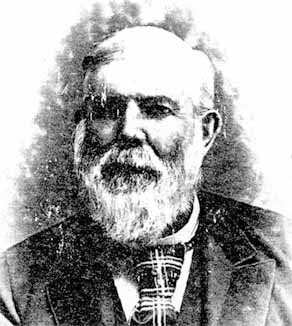
\includegraphics[height=1in]{prologue/pix/shanks.jpg}
  \\
  \protect\label{fig:shanks}\protect\href{https://en.wikipedia.org/wiki/William_Shanks}{William Shanks，1812--1882} % From https://mathshistory.st-andrews.ac.uk/Biographies/Shanks/, PD because of age.
  \protect\end{center}


  一位著名的计算员是 W. Shanks（尚克斯）。
  他的爱好是计算数学常数。
  他于 1873 年发表了将~$\pi$ 计算到小数点后 $707$ 位的结果，但只有前 $527$ 位是正确的。
  （大约在 1820 年，C. Babbage（巴贝奇）设计差分机，正是为了应对由人类计算员完成的对数表计算中的错误。）
  \protect

\begin{center} \protect\small
    \protect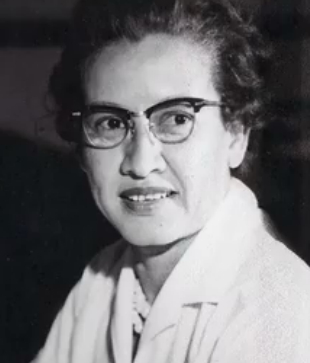
\includegraphics[height=1in]{prologue/pix/katherinejohnson.jpg}
  \\
  \protect\label{fig:johnson}\protect\href{https://bitchmedia.org/article/african-american-women-worked-some-nasas-first-computers}{Katherine Johnson（凯瑟琳·约翰逊），1918--2020，于 2015 年接受总统自由勋章} % NASA/Bill Ingalls, from https://commons.wikimedia.org/wiki/File:Katherine_Johnson_medal.jpeg 
  \protect\end{center}

另一个例子，正如电影《隐藏人物》所述，
多趟美国太空飞行（包括宇航员 John Glenn 的历史性绕地轨道飞行）的轨迹，
都是由人工计算员 Katherine Johnson（凯瑟琳·约翰逊）\protect\index{Johnson, K!picture}和她的同事们通过手算乘法求出的。
她们都是非裔美国女性，她们的成就之所以更加令人敬佩，是因为这是在骇人的歧视之下取得的。}%
正在手工求乘法。
此人遵循一套分步的规程，使用纸笔进行计算，在纸上写满一列列数字。
以此为原型，Turing 为计算员设定了条件。

%<*discussion:DefTuringMachinei>
第一个条件是，它（或者他/她）有一个存储设备（比如计算员的那张纸），可以在上面存放信息，以供后续取用。
% The clerk's paper is two-dimensional but that is
% is not essential, since we could stretch out the work
% into a one-dimensional strip.
%</discussion:DefTuringMachinei>

%<*discussion:DefTuringMachineii>
第二个条件是，这位计算员必须遵循一个确定的程序，一套精确的、不得自由发挥的指令。
程序之所以具有确定性，第一大原因是指令
\citetext{不涉及随机方法}{%
  我们完全可以造出给出纯随机结果的东西；
  例如，有一种装置会记录 Geiger 计数器连续发出的咔咔声，
  如果第二次发出声音间隔比第一次更长，就返回~$1$，
  否则返回~$0$。
  另见
  \protect\url{https://blog.cloudflare.com/randomness-101-lavarand-in-production/}.}，
比如不会通过数放射性衰变产生的咔咔声来决定要执行两种可能操作中的哪一种。

第二大原因是计算员是离散的，它不使用
\citetext{连续方法}{%
  在有计算机之前，工程师有时会使用模拟模型，其中有些规模相当庞大，
  参见 \autocite{wiki:Mississippi}。
  在这类模型中，并不存在什么“第一步、第二步”的概念。}
或
\citetext{模拟设备}{%
  关于计算尺，参见 \autocite{avgeeks}；
  关于列线图，参见 \autocite{wiki:Nomogram}；
  关于海军火控计算机，参见 \autocite{navyreviewer}；
  关于一台更通用的机械计算机，参见 \autocite{vimeo:MechComputer}。
  关于安提基特拉机械装置，参见 \url{https://www.youtube.com/watch?v=qqlJ50zDgeA}。
  关于更现代的设计，请参见
  \url{https://youtu.be/IgF3OX8nT0w?si=hiX4gp9O5QViQCp_} 和
  \url{https://www.youtube.com/watch?v=GVsUOuSjvcg}.}。
因此不存在关于操作精度的疑问，这点不像\citetext{从仪表盘或计算尺读取结果}{%
  假设一个计算的中间结果是 $1.23$。
  如果我们按照分辨率精度只有一位小数的约定从计算尺上读取它，
  那么我们记下~$1.2$。
  将其翻倍得到 $2.4$。
  但将原始数字翻倍 $2\cdot 1.23=2.46$，
  然后四舍五入到一位小数，得到 $2.5$.}那样。
与之相应，计算员也一步一步地工作。
必要时，它可以在完整一步之后暂停，记下自己当前做到哪里
（“正要进位一个 $1$”），过一会儿再接着做。
我们说，在每一时刻，计算员都处于有限多个可能的
\definend{状态}之一，\index{state}
这些状态我们记作 $q_0$、$q_1$、\ldots\sentencespace。
%</discussion:DefTuringMachineii>

%<*discussion:DefTuringMachineiii>
Turing 还增加了第三个条件，这是因为他想研究的是什么东西在原则上是可计算的。
因此，可用存储量
\citetext{不设上限}{%
  这个阐释源自
  \autocite{Rogers}, 第 1--5 页。}。
更准确地说，他不设有限的上限\Dash
如果一次计算眼看就要耗尽存储空间，那存储空间就会
\citetext{自动增长}{%
  也许职员有个助手，或者机器有专人看管。}。
输入或输出的量不设上限，输入和输出之外所需的额外存储（暂存内存）也不设上限。\footnote{%
  确实，撇开云存储不谈，每一台现有的物理计算机的内存都是有限的。
  然而，那个空间极其庞大。
  在本部分，当使用模型设备时，对内存施加限制是一种阻碍，顶多也只是无关紧要。}
同样地，指令的数量也不设上限。
计算在完成前需要执行的步骤数量也不设上限。\footnote{%
  有些作者将像内存量这类资源的可用性描述为“无限”。
  Turing 本人就是这样做的。
  \citetext{读者可能会反对，认为这违背了此定义的目标，
    即对原则上是物理可实现的计算进行建模}{%
     我们都知道有些计算没有自然界限。
     我们小学时学的长除法算法，
     无论是输入或输出的长度，还是可用草稿纸的数量，
     都没有内在的上限。}。% https://cs.stackexchange.com/a/100325/67754
  因此，
  这里的论述换了一种说法：
  这些资源并没有有限的上界。
  不过说真的，怎么表述并不重要。
  两种情况的要点都在于：如果某事物在不设界限时都不可计算，
  那么它在任何物理设备上都不可计算。}
%</discussion:DefTuringMachineiii>

%<*discussion:DefTuringMachineiv>
Turing 还面临最后一个问题：计算员需要有多聪明？
例如，它需要会乘法吗？
我们不需要为乘法做一个特殊功能，因为原则上可以通过重复加法来求乘法。
我们甚至不需要加法，因为我们可以重复加1操作来求加法。
就这样，Turing 将计算员简化到非常基本、易于理解的程度，
直至其操作\citetext{如此基本，以至于我们难以想象它们能被进一步分割}{\autocite{Turing}；\autocite{TuringCorr}}，
同时又保持着强大的能力，足以完成任何原则上可完成之事。
%</discussion:DefTuringMachineiv>

\subsection{定义}
基于这些思考，Turing 设想了一个盒子，盒子里装有机械元件，并配有一条纸带。

\begin{center}
   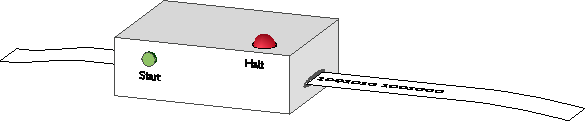
\includegraphics{asy/share/machine00.pdf}
\end{center}

%<*discussion:DefTuringMachinev>
纸带是就是存储器，\index{Turing machine!tape} % \index{memory}
有时也称为“内存”。\index{store, of a machine}
盒子可以从纸带上读取字符，也可以向纸带写入字符，一次一个，
同时还能相对于纸带向任一方向移动读写头\index{read/write head}\index{I/O head|see {read/write head}}\index{Turing machine!read/write head}。
因此，要做乘法的话，
计算员就可以从纸带上读取两个乘数作为输入
（图中显示的是二进制下的
$74$ 和~$72$，中间用空白符隔开），
用纸带做草稿，在计算出结果时停机，并将输出留在纸带上。
%</discussion:DefTuringMachinev>

%<*discussion:DefTuringMachinevi>
盒子就是计算员，也就是 CPU，\index{CPU of Turing machine}\index{Turing machine!CPU}
有时也称为“控制器”。\index{control, of a machine}\index{Turing machine!control}
\texttt{Start}按钮% \index{Start button@\texttt{Start} button}\index{button!start}
用来启动计算。
当计算完成时，
\texttt{Halt}指示灯%\index{Halt light@\texttt{Halt} light}\index{light!Halt@\texttt{Halt}}
会亮起以示停机。
%</discussion:DefTuringMachinevi>
盒子内部的工程实现并不重要\Dash
也许就像我们熟悉的机器那样，它内部有集成电路，
也可能是齿轮和杠杆，又或者是
\index{LEGO}\citetext{乐高积木}{%
  例如参见 \protect\url{https://www.youtube.com/watch?v=RLPVCJjTNgk&t=114s}。}\Dash 重要的是，
它由有限多个部件组成，每个部件
只能处于有限多种状态。
如果它是芯片构成的，那么每个寄存器只有有限多个可能的值；
而如果它是用齿轮或积木搭成的，那么每个部件只能稳定在有限多个可能的位置上。
因此，无论它是如何构造的，
盒子总共只有有限多个状态。

%<*discussion:DefTuringMachinevii>
在执行计算时，机器会逐步从一个状态转移到另一个状态。
例如，
在做乘法时，它可能会根据当前所处的状态以及从纸带上读到的内容，
决定下一步需要进位~$1$。
这时它会转移到一个新状态，
直观上这个新状态就是进行进位操作的地方。

因此，机器的每个步骤涉及四项信息。
我们称
当前状态\index{present state}\index{state!present}\index{Turing machine!present state}为 $q_p$，
下一状态\index{next state}\index{state!next}\index{Turing machine!next state}%
为 $q_n$。
读写头当前指向的符号\index{present tape symbol}\index{Turing machine!present symbol}是 $T_p$。
最后，下一个\index{next tape action}\index{Turing machine!next action}%
纸带动作为~$T_n$。
可能的动作有：在不写入的情况下向左或向右移动读写头，
分别记作 $T_n=\str{L}$ 或~$T_n=\str{R}$，\footnote{%
  我们是
  移动纸带还是移动读写头并不重要，重要的是它们之间的
  相对运动。
  因此 $T_n=\str{L}$ 表示要么纸带、要么读写头移动，使得
  读写头现在指向左侧一格。
  在绘图时，我们保持纸带不动而移动读写头，因为
  这样图形更容易阅读。}
或者在不移动读写头的情况下向纸带写入一个符号，
这时就用该符号表示，因此 $T_n=\str{1}$ 表示机器将向纸带写入一个 \str{1}。
至于字母表，\index{alphabet!tape}\index{tape alphabet@tape alphabet $\Sigma$}\index{input alphabet}
也就是可以出现在纸带上的字符集合，
我们会根据手头的工作选择任何方便的字母表。
但是，
每张纸带上除了有限多个位置外，其余位置都是
空白符\index{blank@blank character \str{B}}\index{tape symbol!blank}，
因此空白符必须是符号之一。
（当空位可能引起混淆时，我们用 $\str{B}$ 表示空白符。）
%</discussion:DefTuringMachinevii>

%<*discussion:DefTuringMachineviii>
这样的四元组 $q_pT_pT_nq_n$ 就是一个\definend{指令}。\index{instruction}\index{Turing machine!instruction}
例如，指令
$\tminstruction{3}{1}{B}{5}$
只有在机器当前处于状态~$q_3$
且正在读取纸带上的符号 \str{1} 时才会执行。
若如此，机器会向纸带写入一个空白符，覆盖掉原来的 \str{1}，
然后转移到状态~$q_5$。
%</discussion:DefTuringMachineviii>

\begin{example} \label{ex:MPred} 
%<*ex:PredecessorTMi>
这台纸带符号集为 $\Sigma=\set{\str{B},\str{1}}$ 的 Turing 机
有六条指令。
\begin{equation*}
 \TM_{\text{pred}}=
  \set{ \tminstruction{0}{B}{L}{1},\,
        \tminstruction{0}{1}{R}{0},\,
        \tminstruction{1}{B}{L}{2},\,
        \tminstruction{1}{1}{B}{1},\,
        \tminstruction{2}{B}{R}{3},\,
        \tminstruction{2}{1}{L}{2} 
      }
\end{equation*}
%</ex:PredecessorTMi>
下方展示了它的一个初始格局。
图中显示了一段纸带，以及机器的状态和读写头的位置。
%<*ex:PredecessorTMii>
\begin{center}
  \tapegraphic{\tmexercises pred000.pdf}
\end{center}
我们采用如下约定：当我们按下 \texttt{Start} 时，机器处于状态 $q_0$。\index{start state@start state $q_0$}\index{state!start}
上图显示机器正在读~$\str{1}$，因此适用指令 $\tminstruction{0}{1}{R}{0}$。
所以第一步是：机器将读写头右移，并保持状态~$q_0$。
%</ex:PredecessorTMii>
下面表格的第一行展示了这一步，
后续行则展示了之后各步的格局。
%<*ex:PredecessorTMiii>
简要来说，读写头先向右滑动，将最后的
\str{1} 置为空白，然后再滑回起点。
\begin{tapesequence}
  \begin{tapesequencetable}
    1 &\tapegraphic{\tmexercises pred001.pdf} \\
    2 &\tapegraphic{\tmexercises pred002.pdf} \\
    3 &\tapegraphic{\tmexercises pred003.pdf} \\
    4 &\tapegraphic{\tmexercises pred004.pdf} \\
    5 &\tapegraphic{\tmexercises pred005.pdf} 
  \end{tapesequencetable}
  \hspace*{2em}
  \begin{tapesequencetable}
    6 &\tapegraphic{\tmexercises pred006.pdf} \\
    7 &\tapegraphic{\tmexercises pred007.pdf} \\
    8 &\tapegraphic{\tmexercises pred008.pdf} \\
    9 &\tapegraphic{\tmexercises pred009.pdf} 
  \end{tapesequencetable}
\end{tapesequence}
至此，由于没有 $q_3\str{1}$ 指令，机器停机。
%</ex:PredecessorTMiii>

%<*ex:PredecessorTMiv>
如果这台机器启动时，初始纸带上除了连续 $n$ 个（$n>0$）\str{1} 外全是空白，且读写头指向其中最左边的那个 \str{1}，那么当机器停机时，纸带上将会有 $n-1$ 个 \str{1}。
如果纸带初始时有 $0$ 个 \str{1}（即全是空白），那么当机器停机时，纸带上也仍是 $0$~个 \str{1}。
也就是说，这台机器计算的是
\definend{前驱函数}\index{predecessor function}\index{function!predecessor}。
\begin{equation*}
  \operatorname{pred}(x)= \begin{cases}
                    x-1  &\case{若 $x>0$}  \\
                    0    &\case{else}
                  \end{cases}
\end{equation*}
%</ex:PredecessorTMiv>
其他示例也延续这一约定：机器启动时读写头指向输入的最左侧符号。
\end{example}

\begin{example} \label{ex:MAdd}
%<*ex:AdditionTMi>
我们可以将这台纸带字母表为 $\Sigma=\set{\str{B},\str{1}}$ 的机器视为在做两个自然数的加法。\index{addition!Turing machine for}\index{Turing machine!for addition}
\begin{align*}
  \TM_{\text{add}} 
  &=
  \{\hspace{\setspacing} \tminstruction{0}{B}{B}{1},\,
        \tminstruction{0}{1}{R}{0},\,
        \tminstruction{1}{B}{1}{1},\,
        \tminstruction{1}{1}{1}{2},\,
        \tminstruction{2}{B}{B}{3},\,        
        \tminstruction{2}{1}{L}{2},\,  \\
        &\qquad\;\tminstruction{3}{B}{R}{3},\,
        \tminstruction{3}{1}{B}{4},\,          
        \tminstruction{4}{B}{R}{5},\,
        \tminstruction{4}{1}{1}{5} 
      \hspace{\setspacing}\}
\end{align*}
输入的两个数字由两串 \str{1} 表示，中间用一个空白符隔开。
%</ex:AdditionTMi>
%<*ex:AdditionTMii>
下图显示了机器准备计算 $2+3$。
\begin{center}
  \tapegraphic{\tmexercises add000.pdf}
\end{center}
%</ex:AdditionTMii>
% We adopt the convention that this is the configuration at step~$0$.
一旦我们按下 \texttt{Start}，机器就向右扫描，
寻找空白分隔符。
它会将那个空白符改写为一个 \str{1}。
接着它掉头向左扫描，直到找到输入的开头。
\citetext{最后，它去掉一个~\str{1}}{%
  指令 $\tminstruction{4}{1}{1}{5}$ 实际上永远不会被触发，
  但这并无妨碍。
  它的存在是为了满足 Turing 机的形式定义，使得
  $\Delta$ 函数在所有的 $q_pT_p$ 上都有定义。
  另请参见该定义的注释。} 
并最终停机，此时读写头指向纸带非空白部分的起始位置。
各步骤如下所示。
%<*ex:AdditionTMiii>
\begin{tapesequence}
  \begin{tapesequencetable}
    1 &\tapegraphic{\tmexercises add001.pdf} \\
    2 &\tapegraphic{\tmexercises add002.pdf} \\
    3 &\tapegraphic{\tmexercises add003.pdf} \\
    4 &\tapegraphic{\tmexercises add004.pdf} \\
    5 &\tapegraphic{\tmexercises add005.pdf} \\
    6 &\tapegraphic{\tmexercises add006.pdf} 
  \end{tapesequencetable}
  \hspace*{2em}
  \begin{tapesequencetable}
     7 &\tapegraphic{\tmexercises add007.pdf} \\
     8 &\tapegraphic{\tmexercises add008.pdf} \\
     9 &\tapegraphic{\tmexercises add009.pdf} \\
    10 &\tapegraphic{\tmexercises add010.pdf} \\
    11 &\tapegraphic{\tmexercises add011.pdf} \\
    12 &\tapegraphic{\tmexercises add012.pdf} 
  \end{tapesequencetable}
\end{tapesequence}
%</ex:AdditionTMiii>
% We can think of this machine as computing the sum of two inputs,  
% $f(x,y)=x+y$.
\end{example}

%<*ex:PredecessorTMv>
除了用列表形式给出机器的指令外，
我们还可以使用表格或图形。
以下是 $\TM_{\text{pred}}$ 的
\definend{转移表}\index{transition table}\index{table, transition}\index{transition function@transition function $\Delta$!table of} 
及其
\definend{转移图}。\index{transition graph}\index{graph!transition}\index{transition function@transition function $\Delta$!graph of}
%</ex:PredecessorTMv>


\begin{center}
  \begin{transitionfunction}[\Delta_{\text{pred}}]
           &$\blank$      &\str{1}        \\ \cline{2-3}
     $q_0$ &$\str{L}q_1$  &$\str{R}q_0$     \\ 
     $q_1$ &$\str{L}q_2$  &$\str{B}q_1$     \\ 
     $q_2$ &$\str{R}q_3$  &$\str{L}q_2$     \\  
     $q_3$ &--            &--     \\
  \end{transitionfunction}
  \hspace{2em}
  \vcenteredhbox{\includegraphics{prologue/asy/circlediagram/circlediagram00.pdf}}
\end{center}


而这是 $\TM_{\text{add}}$ 所对应的表格与图。


\begin{center}
  \begin{transitionfunction}[\Delta_{\text{add}}]
           &$\blank$      &\str{1}        \\ \cline{2-3}
     $q_0$ &$\str{B}q_1$  &$\str{R}q_0$     \\ 
     $q_1$ &$\str{1}q_1$  &$\str{1}q_2$     \\ 
     $q_2$ &$\str{B}q_3$  &$\str{L}q_2$     \\  
     $q_3$ &$\str{R}q_3$  &$\str{B}q_4$     \\  
     $q_4$ &$\str{R}q_5$  &$\str{1}q_5$     \\  
     $q_5$ &--            &--     \\
  \end{transitionfunction}
  \hspace{2em}
  \vcenteredhbox{\includegraphics{prologue/asy/circlediagram/circlediagram01.pdf}}
\end{center}


% The graph is how we will most often present machines that are small 
% but if there are lots of states then it can be visually confusing.

接下来是一个关键观察。
有些 Turing 机，至少对某些起始格局而言，是永不停机的。


\begin{example} \label{ex:TMNeverHalts}
%<*ex:SomeTMsDontHalt>
Turing 机
$
  \TM_{\text{inf loop}}=\set{
        \tminstruction{0}{B}{B}{0},\,
        \tminstruction{0}{1}{1}{0}
      }
$
不论输入是什么都永不停机。
\begin{center}
  \vcenteredhbox{\includegraphics{\asydir circlediagram/infloop.pdf}}
\end{center}
%</ex:SomeTMsDontHalt>
练习中会要求你给出在一些输入上停机、在另一些输入上不停机的 Turing 机例子。
\end{example}

是时候下定义了。
我们将\definend{符号}\index{symbol}\index{tape symbol}定义为设备为了存储和检索而能够写入和读取的事物。\footnote{%
  设备如何做到这一点取决于其具体的构造方式。
  它可以读写纸带上的标记，
  调整塑料磁带上的磁性颗粒排列，
  翻转固态硬盘上的比特位，
  或者将乐高积木推到凹槽的左边或右边。
  离散性要求机器能够清晰地区分不同的符号，而读取接近边界处的仪器刻度盘时则可能会遇到麻烦。}

%<*df:TM>

\begin{definition} \label{def:TuringMachine}
一台\definend{Turing 机（Turing machine）}~$\TM$\index{Turing machine!definition} 
是一个有限的四元组
\definend{指令（instruction）}\index{instruction}\index{Turing machine!instruction} 
集合，指令形如 $q_pT_pT_nq_n$。\footnotemark[2]
在一条指令中，
\definend{当前状态（present state）}~$q_p$\index{present state}\index{Turing machine!present state} 和
\definend{下一状态（next state）}~$q_n$\index{next state}\index{Turing machine!next state} 属于一个
\definend{状态集（set of states）}~$Q$。\index{states!set of Q@set of $Q$} 
\definend{输入符号（input symbol）}\index{symbol!input}\index{Turing machine!input symbol}
或
\definend{当前符号（current symbol）}\index{current symbol}\index{symbol!current}\index{Turing machine!current symbol} 
$T_p$ 属于
\definend{纸带字母表（tape alphabet）}\index{tape alphabet@tape alphabet $\Sigma$}\index{alphabet!tape}\index{alphabet!Turing machine}\index{Turing machine!tape alphabet} 
集合~$\Sigma$，
该集合至少包含两个符号，其中包括一个称为
\definend{空白符（blank）}的符号，\index{blank@blank character \str{B}}
并且不包含 $\str{L}$ 或~$\str{R}$。
\definend{动作符号（action symbol）}~$T_n$\index{symbol!action}\index{Turing machine!action symbol}\index{symbol!action}\index{Turing machine!action symbol} 
属于
\definend{动作集（action set）}~$\Sigma\cup\set{\str{L},\str{R}}$。\index{action set}\index{Turing machine!action set} 

集合~$\TM$ 必须是
\index{determinism}\index{Turing machine!deterministic}\definend{确定性的（deterministic）}：不同的
四元组不能以
相同的 $q_pT_p$ 开头。
因此，在指令集 $q_pT_pT_nq_n\in\TM\!$ 上，
从当前对 $q_pT_p$ 到下一对~$T_nq_n$ 的关联
定义了一个函数，即
\citetext{\definend{转移函数（transition function）}}{%
  定义将 $\Delta$ 描述为一个函数
  $\map{\Delta}{Q\times \Sigma}{(\Sigma\cup\set{\str{L},\str{R}})\times Q}$。
  这其实是一种权宜之计。
  在 $\TM_{\text{pred}}$ 中，状态 $q_3$ 仅用于使机器停机，因此没有定义下一状态。
  在 $\TM_{\text{add}}$ 中，状态~$q_5$ 扮演了同样的角色。
  所以，严格来说，转移函数是一个偏函数（partial function），即其定义域中的某些成员没有对应的
  值；参见第~\pageref{def:PartialFunction}~页。
  （或者，我们可以把状态集写成
  $Q\cup\hat{Q}$，其中 $\hat{Q}$ 里的状态仅用于
  停机，而转移函数的定义为
  $\map{\Delta}{Q\times \Sigma}{(\Sigma\cup\set{\str{L},\str{R}})\times (Q\cup\hat{Q})}$。）
  我们在主要叙述中略去了这一点，
  因为通常不会引起混淆，深入讨论反而可能分散注意力。}\index{transition function@transition function $\Delta$!Turing machine}\index{function!transition}\index{Turing machine!transition function}
或称
\definend{下一状态函数（next-state function）}\index{next-state function|see{transition function}}\index{function!next-state|see{transition function}}\index{Turing machine!next-state function}
$\map{\Delta}{Q\times \Sigma}{(\Sigma\cup\set{\str{L},\str{R}})\times Q}$。 
\end{definition}

\footnotetext[2]{%
  我们用 $\TM$ 来表示 Turing 机，是因为尽管这些机器
  是硬件，
  但它们最像我们日常经验中的程序。}
%</df:TM>

% %<*df:TMnote>
% We denote Turing machines with a $\TM$ because, although they are hardware, 
% the things from everyday experience that they are most like are programs.
% %</df:TMnote>

当然，这些机器的关键在于它们能做什么。
为了完成形式化，我们现在给出
\citetext{对机器动作的完整描述}{%
  一个很合理的问题是：为什么我们的标准模型——Turing 机——
  如此基础，以至于为它编程
  可能很繁琐？
  为什么不选一个真实世界里的机器呢？
  原因是，我们可以用仅仅几段话就完全描述 Turing 机模型的
  动作
  动作。
  而一台真实的机器本身就需要一整本书来描述。
  此外，Turing 机具有历史
  重要性，而且第五章的工作也需要它们。}。

\label{text:DescriptionOfTMAction}
回顾\zcref{ex:MPred}和\zcref{ex:MAdd}的执行过程可以清楚地看到，Turing 机是通过控制机器排布之间的转移来运作的。
%<*def:TMConfigurationi>
Turing 机的一个
\definend{格局（configuration）}\index{configuration!Turing machine}\index{Turing machine!configuration}  
是一个四元组$\sequence{q,s,\tau_L,\tau_R}$，其中
\citetext{$q$ 是一个状态}{% 
  我们对“状态”究竟是什么并未给出严格定义。
  正式的字典定义称其为机器的一种“模式”
  \url{https://www.merriam-webster.com/dictionary/state}，
  但这只是用一个词替换了另一个词。
  为了直观理解，我们可以想象一台由多个齿轮构成的机器。
  那么，状态就是所有可能的齿轮组合，
  例如齿轮四的第六个齿嵌入齿轮五的第七个槽中，使两者啮合。
  在一台笔记本电脑上，状态集由所有可能的寄存器及其内容的组合构成，
  例如寄存器八包含 \str{101010}。}，
$s$ 是来自纸带字母表~$\Sigma$ 的一个字符，
而 $\tau_L$ 和~$\tau_R$ 是来自~$\kleenestar{\Sigma}\!$ 的串，
也可能是空串~$\emptystring$。\index{empty string@empty string, $\emptystring$}\index{string!empty}
它们分别表示当前状态、读写头下的字符、以及读写头左侧和右侧的纸带内容。
%</def:TMConfigurationi>
例如，在\zcref{ex:MAdd}的跟踪表中，
“步骤~$2$” 这一行显示，经过两次转移后，
状态是 $q=q_0$，
读写头下的字符是空白符 $s=\str{B}$，
读写头左侧是 $\tau_L=\str{11}$，
读写头右侧是 $\tau_R=\str{111}$。
因此，该行的图示描绘了格局
$\sequence{q_0,\str{B},\str{11},\str{111}}$。
换句话说，格局是
\citetext{一个快照，即计算中的一个瞬间}{%
  因此，格局连同 Turing 机就是你继续该计算所需的所有信息\Dash 它封装了该计算的未来历史。}。

\label{DefnConfiguration}
%<*def:TMConfigurationii>
我们用 $\configuration(t)$ 表示机器在第 $t$ 次转移后的格局，并称之为
\definend{步骤}~$t$ 时的格局。\index{step of a computation}\index{computation!step}
我们将此定义扩展到步骤~$0$，规定
\definend{初始格局（initial configuration）}\index{initial configuration!Turing machine}\index{configuration!initial!Turing machine} 
$\configuration(0)$
是我们在按下 \texttt{Start} 键之前机器的格局。
%</def:TMConfigurationii>

接下来定义其动作：假设在步骤~$t$，
机器 $\TM$ 处于格局
$\configuration(t)=\sequence{q,s,\tau_L,\tau_R}$。
为了进行下一次转移，寻找一条
形如 $q_pT_pT_nq_n\in\TM$ 的指令，其中
$q_p=q$ 且~$T_p=s$。
确定性条件确保了集合~$\TM$ 中至多有一条这样的指令。
如果没有这样的指令，那么在
步骤~$t+1$，机器 $\TM$ 就会\definend{停机（halts）}。
此时的格局就是它的
\definend{停机格局（halting configuration）}。\index{halting configuration!Turing machine}\index{configuration!halting!Turing machine}\index{Turing machine!halting configuration}

否则，有三种可能性。
(1)~如果 $T_n$ 是纸带字母表集合~$\Sigma$ 中的一个符号，那么
机器将该符号写入纸带，因此
下一个格局是
$\configuration(t+1)=\sequence{q_n,T_n,\tau_L,\tau_R}$，其定义如下。
(2)~如果 $T_n=\str{L}$，那么机器将读写头向左移动。
更准确地说，下一个格局是  
$\configuration(t+1)=\sequence{q_n,\hat{s},\hat{\tau}_L,\hat{\tau}_R}$。
% where $\hat{s}$ is the rightmost character of the string~$\tau_L$,
% where $\hat{\tau}_R$ is the result of pushing the character~$s$
% onto the string~$\tau_R$,
% and where $\hat{\tau}_L$ is $\tau_L$ with its rightmost character omitted.
% (More precisely,
其新的右侧纸带 
$\hat{\tau}_R$ 是由单字符的串
$\sequence{s}$ 与先前格局的 $\tau_R$ 拼接而成。
至于 $\configuration(t+1)$ 的新左侧纸带和新的当前
字符，有两种情况：当 
$\tau_L=\emptystring$ 时，$\hat{s}$ 是空白符
且 $\hat{\tau}_L=\emptystring$，
而当 $\tau_L\neq\emptystring$ 时，新的当前字符 $\hat{s}$ 是  
$\tau_L$ 的最右字符，即 $\hat{s}=\tau_L[-1]$， 
而新的左侧纸带 $\hat{\tau}_L$ 
则是 $\tau_L$ 去掉最右字符后余下的部分，即
$\hat{\tau}_L=\tau_L[\,:-1]$。
(3)~如果 $T_n=\str{R}$，那么机器将读写头向右移动。
这与~(2) 非常相似，故省略细节。

%<*def:TMConfigurationiii>
如果两个格局通过一步转移相关联，
那么我们记作
$\mathcal{C}(i) \yields \mathcal{C}(i+1)$。\footnote{% 
  将 `$\,\yields$' 读作“转移为”。
  % We could, where $\mathcal{I}$ is the applicable instruction,
  % write~$\yields_{\mathcal{I}}$,  
  % but we will never need to do that.
  }\index{yields@yields $\yields$!for Turing machines}
一个\definend{计算（computation）}\index{computation!Turing machine}\index{Turing machine!computation} 
是一个序列
$
  \mathcal{C}(0) \yields \mathcal{C}(1) \yields \mathcal{C}(2)
   \yields \cdots\, 
$。
我们用 $\kleenestar{\yields}$ 来缩写一连串的 $\yields$。\footnote{% 
  读作“最终转移为”。} %\index{yields eventually!$\kleenestar{\yields}$for Turing machines} 
如果计算停机，那么序列有一个最终的
格局~$\mathcal{C}(h)$ 
因此我们可以将一次停机计算写作
$\mathcal{C}(0)\mathrel{\kleenestar{\yields}}\mathcal{C}(h)$。
%</def:TMConfigurationiii>

\begin{example} \label{ex:TraceComputation}
  在\zcref{ex:MPred}追踪机器步骤的表格中，图形展示了相继的格局
  （注意初始图形在表格之前）。
下面将同一序列展示为一个计算。
\begin{multline*}
\sequence{q_0,\str{1},\emptystring,\str{11}}
\yields
\sequence{q_0,\str{1},\str{1},\str{1}}
\yields
\sequence{q_0,\str{1},\str{11},\emptystring}
\yields
\sequence{q_0,\str{B},\str{111},\emptystring}
\yields
\sequence{q_1,\str{1},\str{11},\emptystring}  \\
\yields
\sequence{q_1,\str{B},\str{11},\emptystring}
\yields
\sequence{q_2,\str{1},\str{1},\emptystring}
\yields
\sequence{q_2,\str{1},\emptystring,\str{1}}
\yields
\sequence{q_2,\str{B},\emptystring,\str{11}}
\yields
\sequence{q_3,\str{1},\emptystring,\str{1}}
\end{multline*}
\end{example}

关于这些细节，还有最后一点。
我们已经将计算定义为一个物理系统通过一系列离散步骤演化的过程。
\citetext{注意，这种演化是局部的，因为所有动作都发生在读写头所在的一个单元格内}{%
    改编自 \autocite{WigdersonMC}。}。

% Finally, as in that example,
% observe that our description of the action of a Turing machine
% emphasizes that it is a
% \citetext{\index{state machine}}{%
%   A state machine is a device that stores the status of something at a
%   given time.
%   On input it can change the status (it can also cause an action or
%   output to take place).
%   Mathematically, it is a finite set $Q=\set{q_0,\ldots q_n}$ along with
%   a function $\map{\Delta}{Q\times\Sigma}{Q}$.}\index{machine!state}\definend{state machine}\Dash
% a computation is a sequence of discrete transitions.

\subsection{可计算函数}\index{computable function|(}
在本章开头我们曾表示，相对于计算如何进行，我们对机器计算出的东西更感兴趣。\footnote{%
  这与编程课程形成对比，编程课需要投入大量精力学习如何将复杂任务分解为更简单的子任务，如何在子任务间建立可靠的接口等。}
本节最后，我们将定义可以被机械计算的函数集合。

%<*df:FcnComputedByTMi>
函数是输入与输出之间的一种关联。
对于 Turing 机，自然的关联是：将机器启动时纸带上的串与它停机时纸带上的串联系起来。
这样我们就得到了一个从串到串的函数，如
$\TMfcn(\str{111})=\str{11111}$，就像这里一样。
\begin{equation*}
 \vcenteredhbox{\includegraphics{\asydir tape/tapefcn0.pdf}} 
  \quad\mapsto\quad
  \vcenteredhbox{\includegraphics{\asydir tape/tapefcn1.pdf}}
\end{equation*}
%</df:FcnComputedByTMi>
\noindent
但该定义必须注意几个问题。
首先，Turing 机可能在某些输入串上不停机。
其次，
仅仅指定输入串还不够，因为读写头的初始位置会影响计算。

%<*df:FcnComputedByTMii>


\begin{definition} \label{def:FcnComputedByTM}
  设 $\TM$ 是一台纸带字母表为 $\Sigma$ 的 Turing 机。
  对于输入 $\sigma\in\kleenestar{\Sigma}\!$，
  将该串放置在其他位置均为空白的纸带上，并将 $\TM$ 的读写头指向 $\sigma$ 最左边的符号，这一过程称为对该输入的
  \definend{装载}\index{loading input on tape}\index{input!loading}。
  如果我们以装载好 $\sigma$ 的状态启动 $\TM$ 且它最终停机，
  那么我们将关联的输出串记作
  \definend{$\TMfcn_{\TM}(\sigma)$}。
  如果机器永不停机，则 $\sigma$ 没有关联的输出。
\definend{机器计算的函数}~$\TM$\index{function!computed by a Turing machine}\index{Turing machine!function computed}
  是所有关联 $\sigma \mapsto \TMfcn_{\TM}(\sigma)$ 的集合。
\end{definition}


%</df:FcnComputedByTMii>

%<*df:FcnConverge>


\begin{definition}
对于 $\sigma\in\kleenestar{\Sigma}\!$，
如果 Turing 机计算的值在 $\sigma$ 上没有定义，
那么我们称机器计算的函数在该输入上
\definend{发散}，\index{diverge}\index{function!diverge}
记作\definend{$\TMfcn_{\TM}(\sigma)\mathord{\uparrow}$}
（或 $\TMfcn_{\TM}(\sigma)=\bot$\,）。
否则我们称它在该输入上
\definend{收敛}，\index{converge}\index{function!converge}
\definend{$\TMfcn_{\TM}(\sigma)\mathord{\downarrow}$}。
\end{definition}


%</df:FcnConverge>

%<*discussion:FcnVsMachine>
注意区分机器 $\TM$ 和该机器计算的函数 $\TMfcn_{\TM}$。
例如，
机器 $\TM_{\text{pred}}$ 是一个四元组的集合，
但前驱函数是一个输入-输出对的集合，
我们可以将其记作 $x\mapsto \operatorname{pred}(x)$。
另一个区别的例子是：机器停机或不停机，而函数收敛或发散。
%</discussion:FcnVsMachine>

还有几点：


\begin{parenum}
\item
当讨论中只有一台机器时，我们写作 $\TMfcn$ 来代替 $\TMfcn_{\TM}$。
\item
在本书中，我们倾向于构造这样的机器，使其在结束时读写头也位于输出串的第一个字符下方，
这并非严格必要，但使得组合机器更容易。
\item
在大多数数学领域中，函数都有一个定义域，即其有定义的那些输入构成的集合。
在本领域，一个关键特性是机器可以接收一个输入串，却永不返回输出，因为它不停机。
因此在这里，我们常写作
$\map{\phi}{\kleenestar{\Sigma}}{\kleenestar{\Sigma}}$
并将其描述为一个
\definend{偏函数}，\index{partial function}\index{function!partial}
其中某个
$W\subseteq\kleenestar{\Sigma}$ 是所有使得 $\phi(\sigma)\converges$ 的输入串 $\sigma$ 的集合。
如果 $W=\kleenestar{\Sigma}$，则称 $\phi$ 是一个
\definend{全函数}。\index{total function}\index{function!total}
（每个 $\phi$ 都是偏的，但说“偏”通常意味着该函数不是全的。）\footnote{%
  更多内容参见附录~\protect\ref{sec:Functions}。}
\end{parenum}

% There is one last point to raise about the definition.
%<*discussion:FcnConverge>
我们常常会考虑那些并非从串到串的映射的函数，并将它们描述为由机器计算的函数。
为此，我们必须对输入和输出赋予一种解释。
一个例子是\zcref{ex:MPred}中的前驱机，在那里我们把串解释为一元表示的自然数。
% The same holds for computations with non-numbers.
% \footnote{%
%   In the example of the addition machine, \protect\zcref{ex:MAdd},
%   we took the separator blank to be significant.
%   Allowing significant blanks
%   opens the possibility of ambiguity:~which of the 
%   blanks at the beginning and end of the input and output strings
%   count and which do not?
%   There are a number of ways that we could handle this.
%   We could add a character to the alphabet to use exclusively as a begin/end
%   marker.
%   Or we could enforce that strings
%   come in the form $\sigma=1^n\str{B}\tau$
%   where the length of $\tau$ is~$n$
%   (so that any time we change $\tau$'s length we
%   must adjust the~$n$).
%   Perhaps the most mathematically pleasant is to  
%   code everything that we want to say with integers, in unary.
%   Thus, we could code the triple of numbers $\sequence{7, 8, 9}$
%   as the
%   single number $2^7 3^8 5^9\!$, using the uniqueness of
%   prime factorization.
%   In this book
%   we leave off this disambiguation because
%   it hides the underlying ideas (see 
%   also \zcref{rem:EarlyResearchersAirtightArgs}).
% }
% The machine just runs, it is up to us to give the actions a sense.
当然，物理计算机上也发生着同样的事情，机器摆弄着比特串，然后我们将它们解释为文档中的字符、四重奏中的音符，或者任何我们喜欢的东西。\footnote{%
  我们或许会担心，我们的解释可能会变得如此复杂，以至于像占星术一样，实际工作都发生在解释过程中。
  但我们将坚持讨论像自然数的一元表示法这样不存在这一问题的情况。}

当我们描述由机器计算的函数时，我们通常会省略解释串的部分。
我们会说，“这表明 $\TMfcn(3)=5$”
\citetext{而不是说，“这表明 $\TMfcn$ 将一个代表~$3$ 的串映射为一个代表~$5$ 的串。”}{%
  也就是说，我们这样做，理由和我们说“这是我十岁的时候”
  而不是说“这是我十岁时的一张照片”一样。}
表示的细节通常在这一章里无关紧要
（在第五章，我们有时会关心它们消耗的时间或空间）。
%</discussion:FcnConverge>

\begin{remark} \label{rem:EarlyResearchersAirtightArgs}
早期的研究者在实际机器尚未普及之前工作，他们需要严密的证明，例如，存在一种机械计算，能够计算这样的函数：输入一个数，返回该数素数分解中 $5$ 的幂次。
因此他们处理了这些细节，积累了大量可能相当底层的工作成果。

作为一个底层细节的例子，在加法机\zcref{ex:MAdd}中，我们把分隔用的空白符视为有意义的。
允许有意义的空白符带来了歧义性问题：纸带上哪些空白符算作输入和输出，哪些不算？
我们可以通过给字母表增加一个专门用作开始/结束标记的字符来处理。
或者，我们可以强制要求串以 $\sigma=\alpha\str{B}\tau$ 的形式出现，其中 $\tau$ 由 $\lh{\alpha}$ 个 \str{1} 组成。
又或者，我们可以用整数编码一切，例如将三元组 $\sequence{7, 8, 9}$ 编码为 $2^7 3^8 5^9\!$。

在本书中，我们通常不坚持这种细节程度。
我们的日常经验使我们相信，机器可以用它们的字母表合理地表示任何可计算的东西。
此外，在细节上花费大量时间有掩盖核心思想的风险，而我们希望进入更有趣的内容。
下一节会对此有更多说明。
\end{remark}

%<*df:ComputableFcn>


\begin{definition} \label{def:ComputableFcn}
一个\definend{可计算函数},\index{computable function!definition}\index{function!computable} 
或 \index{recursive function}\index{function!recursive}\definend{递归函数},\footnotemark[1]
是由某个 Turing 机计算的函数（它可以是全函数或偏函数）。
一个\definend{可计算集},\index{computable set}\index{set!computable} 
或\definend{递归集},\index{recursive set}\index{set!recursive} 
是其特征函数可计算的集合。
一个关系是可计算的\index{computable relation}\index{relation, computable}，当且仅当它作为集合是可计算的。\footnotemark[2]
\end{definition}

\footnotetext[1]{%
  “递归”这个术语曾经是通用的，但现在已有些过时。}
\footnotetext[2]{%
  例如，“小于”关系是可计算的，因为存在一个可计算函数，输入两个整数 $a$ 和~$b$，如果 $a<b$ 则返回~\str{1}，否则返回 \str{0}。}
%</df:ComputableFcn>

% There is a terminology focused on Boolean functions that we will
% emphasize in Chapter Five.

%<*df:TMDecidesLanguage>

\begin{definition} \label{df:TMDecidesLanguage}
若一台 Turing 机计算某集合的特征函数，则称它
\definend{判定}此集合。\index{Turing machine!decide a set}\index{set!decided by a Turing machine}
也就是说，对于所有属于该集合的输入，机器都停机并接受
（或许通过纸带最终只留下 \protect{\str{1}} 来表示），
而对于所有不属于该集合的输入，机器都停机并拒绝
（或许纸带最终全是空白）。\index{Turing machine!decide a language}\index{language!decided by a Turing machine}\index{decides!a language}
若一台 Turing 机对于所有属于某集合的输入都停机并接受，而对于非成员输入，
它从不以接受状态停机（但它可能不停机），则称它\definend{识别}
此集合。\index{Turing machine!recognize a set}\index{set!recognized by a Turing machine}\index{recognized set}
\end{definition}

%</df:TMDecidesLanguage>

\medskip
最后我们总结一下。
我们已经为直观上的机械可计算性给出了一个精确的定义，
从而精确刻画了哪些函数能够被机械计算。
下一小节将讨论为什么这一刻画被广泛接受。
\index{computable function|)}

% -------------------------------------------
\begin{exercises}[除非练习题另有说明，
假设 $\Sigma=\set{\str{B},\str{1}}$。
同时假设任何机器都必须将其读写头起始位置放在最左输入字符下方，
并使其在完成时读写头位于最左输出字符下方。]

\begin{exercise}
Turing 机在哪些方面像一个程序？
在哪些方面不像？
在哪些方面像我们桌上的那种电脑？
在哪些方面不像？
\begin{answer}
它像程序的地方在于它是单一用途的，也就是说，
就像我们可以有一个仅将输入翻倍而不做其他事情的程序一样，
我们也可以有这样一个 Turing 机。
它不像程序的地方在于它是硬件。

它像我们今天桌上电脑的地方在于它机械地将输入转换为输出。
Turing 机不像这种电脑的地方在于它是为单一任务而特制的。
\end{answer}
\end{exercise}

\begin{exercise}
\begin{credit}
  SE 用户 Shuzheng, https://cs.stackexchange.com/q/45589/50343
\end{credit}
为什么 Turing 机的定义（\zcref{def:TuringMachine}）不包括对纸带内容的定义？
% It includes the tape alphabet~$\Sigma$, but not the sequence of alphabet 
% characters that make up the tape.
\begin{answer}
这个定义描述的是机器本身。
关于机器动作的进一步描述，包括格局和转移的定义，
紧随\zcref{def:TuringMachine}之后。
在某种程度上，这是对\zcref{def:TuringMachine}的扩展。

换言之，正如 A~Bauer 在 Stack Exchange 上对此问题的评论中所说，
为什么道路不是汽车的一部分？
\end{answer}
\end{exercise}

\begin{exercise}
\begin{credit}
  问题由 SE 用户 Arsalan MGR 提出，\url{https://cs.stackexchange.com/q/135343/50343}
\end{credit}
你的学习伙伴问道：
“开篇段落提到\textit{Entscheidungsproblem}，即机械地判定一个数学陈述是真还是假。
我经常写带有布尔判断子句的程序，比如‘\texttt{if (x>3)}’。
这有什么问题呢？”
请帮他们解惑。\index{Entscheidungsproblem@\textit{Entscheidungsproblem}}\index{decision problem}
\begin{answer}
这并不是判断某个特定数学陈述是否为真的问题。
显然，如果 $x=2$，那么我们就可以判断 $x>3$ 是否成立。
类似地，我们可以判定 $\forall x\in\N\;[x^2>3]$ 的真假。
而\textit{Entscheidungsproblem} 要求的是一个算法，
它能输入任意数学陈述，并输出 `\true' 或 `\false'。
\end{answer}
\end{exercise}

\recommended

\begin{exercise}
像\zcref{ex:TraceComputation}中那样，追迹下列每次计算。
\begin{exparts*}
\item
追迹例~\ref{ex:MPred}中的机器 $\TM_{\text{pred}}$ 在含有两个 \str{1} 的纸带上启动时的计算。
\item
追迹例~\ref{ex:MAdd}中的机器 $\TM_{\text{add}}$ 在两个加数分别为 $2$ 和~$2$ 时的计算。
\item 如\zcpageref{DefnConfiguration}页所述，以格局序列的形式给出这两个计算。
\end{exparts*}
\begin{answer}
\begin{exparts}
\item 以下是计算 $2$ 的前驱过程中产生的纸带序列。
\begin{tapesequence}
  \begin{tapesequencetable}
    0 &\tapegraphic{\tmexercises pred_two000.pdf} \\
    1 &\tapegraphic{\tmexercises pred_two001.pdf} \\
    2 &\tapegraphic{\tmexercises pred_two002.pdf} \\
  \end{tapesequencetable}
  \hspace*{2em}
  \begin{tapesequencetable}
    3 &\tapegraphic{\tmexercises pred_two003.pdf} \\
    4 &\tapegraphic{\tmexercises pred_two004.pdf} \\
    5 &\tapegraphic{\tmexercises pred_two005.pdf} \\
  \end{tapesequencetable}
  \hspace*{2em}
  \begin{tapesequencetable}
    6 &\tapegraphic{\tmexercises pred_two006.pdf} \\
    7 &\tapegraphic{\tmexercises pred_two007.pdf} \\
  \end{tapesequencetable}
\end{tapesequence}
\item 这是 $2$ 与~$2$ 求和的纸带图序列。
\begin{tapesequence}
  \begin{tapesequencetable}
    0 &\tapegraphic{\tmexercises addtwotwo000.pdf} \\
    1 &\tapegraphic{\tmexercises addtwotwo001.pdf} \\
    2 &\tapegraphic{\tmexercises addtwotwo002.pdf} \\
    3 &\tapegraphic{\tmexercises addtwotwo003.pdf} \\
    4 &\tapegraphic{\tmexercises addtwotwo004.pdf} \\
  \end{tapesequencetable}
  \hspace*{2em}
  \begin{tapesequencetable}
    5 &\tapegraphic{\tmexercises addtwotwo005.pdf} \\
    6 &\tapegraphic{\tmexercises addtwotwo006.pdf} \\
    7 &\tapegraphic{\tmexercises addtwotwo007.pdf} \\
    8 &\tapegraphic{\tmexercises addtwotwo008.pdf} \\
    9 &\tapegraphic{\tmexercises addtwotwo009.pdf} \\
  \end{tapesequencetable}
  \hspace*{2em}
  \begin{tapesequencetable}
   10 &\tapegraphic{\tmexercises addtwotwo010.pdf} \\
   11 &\tapegraphic{\tmexercises addtwotwo011.pdf} \\
   12 &\tapegraphic{\tmexercises addtwotwo012.pdf} \\
  \end{tapesequencetable}
\end{tapesequence}
\item 以下是前驱计算的格局序列。
\begin{align*}
  &\sequence{q_0,\str{1},\emptystring,\str{1}}
   \yields\sequence{q_0,\str{1},\str{1},\emptystring}
   \yields\sequence{q_0,\str{B},\str{11},\emptystring}
   \yields\sequence{q_1,\str{1},\str{1},\emptystring}
   \yields\sequence{q_1,\str{B},\str{1},\emptystring}
   \yields\sequence{q_2,\str{1},\emptystring,\emptystring}  \\
   &\qquad\yields\sequence{q_2,\str{B},\emptystring,\str{1}} 
   \yields\sequence{q_3,\str{1},\emptystring,\emptystring}
\end{align*}
由于状态 $q_3$ 没有对应的指令，因此 $\sequence{q_3,\str{1},\emptystring,\emptystring}$ 是一个停机格局。

$2$ 与 $2$ 相加的计算序列稍长一些。
\begin{align*}
   &\sequence{q_0,\str{1},\emptystring,\str{1B11}}
   \yields\sequence{q_0,\str{1},\str{1},\str{B11}}
   \yields\sequence{q_0,\str{B},\str{11},\str{11}}
   \yields\sequence{q_1,\str{B},\str{11},\str{11}}
   \yields\sequence{q_1,\str{1},\str{11},\str{11}}  \\  
   &\qquad\yields\sequence{q_2,\str{1},\str{11},\str{11}}
   \yields\sequence{q_2,\str{1},\str{1},\str{111}}  
   \yields\sequence{q_2,\str{1},\emptystring,\str{1111}}
   \yields\sequence{q_2,\str{B},\emptystring,\str{11111}}  \\  
   &\qquad\yields\sequence{q_3,\str{B},\emptystring,\str{11111}}
   \yields\sequence{q_3,\str{1},\emptystring,\str{1111}}
   \yields\sequence{q_4,\str{B},\emptystring,\str{1111}}
   \yields\sequence{q_5,\str{1},\emptystring,\str{111}}
\end{align*}
\end{exparts}
\end{answer}
\end{exercise}

\recommended

\begin{exercise}
对于下列关于 Turing 机的错误陈述，简要指出其谬误所在。
\begin{exparts*}
\item Turing 机不能处理负数，因此它不是一个完备的计算模型。
\item \zcref{ex:TMNeverHalts}中的问题在于，指令中没有额外的状态让机器去停机。
\item 一台机器要达到状态 $q_{50}$，它必须至少运行五十一步。
\end{exparts*}
\begin{answer}
\begin{exparts}
\item 要证明对负数（或其他任何数学对象）的某些操作是可计算的，需要先为它们指定一种基于有限字母表上字符串的表示方法，然后展示如何使用 Turing 机对这些字符串进行机械计算。
例如，要证明两个整数的乘法是机械的，我们可以使用字母表 $\Sigma=\set{\str{B},\str{0},\ldots \str{9},\str{+},\str{-}}$ 并将每个整数表示为一对 $\sequence{\text{sign},\text{自然数}}$。构造一台 Turing 机来处理四种可能的符号组合情况，虽然繁琐但完全可行。
\item 如果这里说的“问题”是指机器不停机，那么这并不是问题的根源。相反，这台机器只是一个简单的无限循环。
\item 我们可以给机器设定非顺序编号的状态。唯一的限制是我们遵循初始状态为 $q_0$ 的约定。例如，机器 $\TM=\set{\tminstruction{0}{B}{B}{50},\,\tminstruction{0}{1}{1}{50},\,\tminstruction{50}{1}{1}{1},\,\tminstruction{50}{1}{1}{1}}$ 符合定义，并且在任何输入下都能一步到达状态 $q_{50}$。
\end{exparts}
\end{answer}
\end{exercise}

% \begin{exercise} % From https://cs.stackexchange.com/q/45589/67754
% Why does the definition of a Turing machine, \zcref{def:TuringMachine},
% not mention the tape?
% It mentions the tape alphabet, but not the tape.
% \begin{answer}
% The tape is part of the configuration.
% That is, the paragraphs after the definition describe how the machine
% hardware interacts with the tape to produce a computation
% \end{answer}
% \end{exercise}

\begin{exercise}
有些作者会显式地将 Turing 机定义为拥有
\definend{停机状态}，\index{halting state}\index{state!halting}，
机器进入此状态纯粹是为了停机。
在这种情况下，其他状态就称为
\definend{工作状态}。\index{working state}\index{state!working}
我们的定义虽不要求区分，但书中的很多例子都使用了这一做法。
例如，在\zcref{ex:MPred}中，$q_3$ 是停机状态，其工作状态是 $q_0$、$q_1$ 和~$q_2$。
请指出\zcref{ex:MAdd}中的停机状态和工作状态。
\begin{answer}
停机状态是~$q_5$，工作状态是 $q_0$、$q_1$、$q_2$、$q_3$ 和 $q_4$。
\end{answer}
\end{exercise}

\recommended


\begin{exercise}
从一张空白纸带开始，跟踪\zcref{ex:TMNeverHalts}中机器 $\TM_{\text{inf loop}}$ 执行十步的过程。
% Show the sequence of tapes.
\begin{answer}
跟踪过程并不太有趣。
\begin{tapesequence}
  \begin{tapesequencetable}
    0 &\tapegraphic{\tmexercises infloop000.pdf} \\
    1 &\tapegraphic{\tmexercises infloop001.pdf} \\
    2 &\tapegraphic{\tmexercises infloop002.pdf} \\
    3 &\tapegraphic{\tmexercises infloop003.pdf} \\
  \end{tapesequencetable}
  \hspace*{2em}
  \begin{tapesequencetable}
    4 &\tapegraphic{\tmexercises infloop004.pdf} \\
    5 &\tapegraphic{\tmexercises infloop005.pdf} \\
    6 &\tapegraphic{\tmexercises infloop006.pdf} \\
    7 &\tapegraphic{\tmexercises infloop007.pdf} \\
  \end{tapesequencetable}
  \hspace*{2em}
  \begin{tapesequencetable}
    8 &\tapegraphic{\tmexercises infloop008.pdf} \\
    9 &\tapegraphic{\tmexercises infloop009.pdf} \\
   10 &\tapegraphic{\tmexercises infloop010.pdf} \\
  \end{tapesequencetable}
\end{tapesequence}
\end{answer}
\end{exercise}

\begin{exercise}  % mystery machine
对下面给出的每个输入，跟踪这台 Turing 机
% with alphabet $\Sigma=\set{\str{B},\str{0},\str{1}}$
的执行过程，最多十步（若提前停机则少于十步）。
\begin{equation*}  % Go to q3 if input contains 101, else go to q4
 % \TM=
  \set{ \tminstruction{0}{B}{B}{4},\,
        \tminstruction{0}{0}{R}{0},\,
        \tminstruction{0}{1}{R}{1},\,
        \tminstruction{1}{B}{B}{4},\,
        \tminstruction{1}{0}{R}{2},\,
        \tminstruction{1}{1}{R}{0},\, 
        \tminstruction{2}{B}{B}{4},\,
        \tminstruction{2}{0}{R}{0},\,
        \tminstruction{2}{1}{R}{3} 
      }
\end{equation*}
\begin{exparts*}
\item \str{11}
\item \str{1011}
\item \str{110}
\item \str{1101}
\item \emptystring
\end{exparts*}
\begin{answer}
\begin{exparts}
\item 在这台神秘机器上输入~\str{11} 的运行结果如下。
\begin{tapesequence}
  \begin{tapesequencetable}
    0 &\tapegraphic{\tmexercises mystery11000.pdf} \\
    1 &\tapegraphic{\tmexercises mystery11001.pdf} \\
  \end{tapesequencetable}
  \hspace*{2em}
  \begin{tapesequencetable}
    2 &\tapegraphic{\tmexercises mystery11002.pdf} \\
    3 &\tapegraphic{\tmexercises mystery11003.pdf} \\
  \end{tapesequencetable}
\end{tapesequence}
\item 输入~\str{1011} 时，结果如下。
\begin{tapesequence}
  \begin{tapesequencetable}
    0 &\tapegraphic{\tmexercises mystery1011000.pdf} \\
    1 &\tapegraphic{\tmexercises mystery1011001.pdf} \\
  \end{tapesequencetable}
  \hspace*{2em}
  \begin{tapesequencetable}
    2 &\tapegraphic{\tmexercises mystery1011002.pdf} \\
    3 &\tapegraphic{\tmexercises mystery1011003.pdf} \\
  \end{tapesequencetable}
\end{tapesequence}
\item 输入~\str{110} 时，结果如下。
\begin{tapesequence}
  \begin{tapesequencetable}
    0 &\tapegraphic{\tmexercises mystery110000.pdf} \\
    1 &\tapegraphic{\tmexercises mystery110001.pdf} \\
    2 &\tapegraphic{\tmexercises mystery110002.pdf} \\
  \end{tapesequencetable}
  \hspace*{2em}
  \begin{tapesequencetable}
    3 &\tapegraphic{\tmexercises mystery110003.pdf} \\
    4 &\tapegraphic{\tmexercises mystery110004.pdf} \\
  \end{tapesequencetable}
\end{tapesequence}
\item 输入~\str{1101} 时，机器给出了如下的纸带序列。
\begin{tapesequence}
  \begin{tapesequencetable}
    0 &\tapegraphic{\tmexercises mystery1101000.pdf} \\
    1 &\tapegraphic{\tmexercises mystery1101001.pdf} \\
    2 &\tapegraphic{\tmexercises mystery1101002.pdf} \\
    3 &\tapegraphic{\tmexercises mystery1101003.pdf} \\
  \end{tapesequencetable}
  \hspace*{2em}
  \begin{tapesequencetable}
    4 &\tapegraphic{\tmexercises mystery1101004.pdf} \\
    5 &\tapegraphic{\tmexercises mystery1101005.pdf} \\
  \end{tapesequencetable}
\end{tapesequence}
\item 当初始纸带为空时，运行情况如下。
\begin{tapesequence}
  \begin{tapesequencetable}
    0 &\tapegraphic{\tmexercises mysteryempty000.pdf} \\
    1 &\tapegraphic{\tmexercises mysteryempty001.pdf} \\
  \end{tapesequencetable}
\end{tapesequence}
\end{exparts}
\end{answer}
\end{exercise}

\recommended

\begin{exercise}
给出前一习题中机器的转移表。
\begin{answer}
这是转移表。
\begin{display}
  \begin{transitionfunction}
           &$\blank$      &\str{0}      &\str{1}        \\ \cline{2-4}
     $q_0$ &$\str{B}q_4$  &$\str{R}q_0$ &$\str{R}q_1$     \\ 
     $q_1$ &$\str{B}q_4$  &$\str{R}q_2$ &$\str{R}q_0$    \\ 
     $q_2$ &$\str{B}q_4$  &$\str{R}q_0$ &$\str{R}q_3$    \\  
     $q_3$ &--            &--           &--            \\
  \end{transitionfunction}
\end{display}
\end{answer}
\end{exercise}

\recommended


\begin{exercise}
写一个 Turing 机，如果它启动时纸带上除了一串 \str{1} 外均为空白符，则将这些 \str{1} 替换为空白符，然后停机。
\begin{answer}
机器 $\TM_{\text{blankones}}=\set{
     \tminstruction{0}{B}{B}{2},\,
     \tminstruction{0}{1}{B}{1},\,
     \tminstruction{1}{B}{R}{0},\,
     \tminstruction{1}{1}{1}{0}
}$ 在包含两个 \str{1} 的纸带上的运行过程如下。
\begin{tapesequence}
  \begin{tapesequencetable}
    0 &\tapegraphic{\tmexercises blankones000.pdf} \\
    1 &\tapegraphic{\tmexercises blankones001.pdf} \\
    2 &\tapegraphic{\tmexercises blankones002.pdf} \\
  \end{tapesequencetable}
  \hspace*{2em}
  \begin{tapesequencetable}
    3 &\tapegraphic{\tmexercises blankones003.pdf} \\
    4 &\tapegraphic{\tmexercises blankones004.pdf} \\
    5 &\tapegraphic{\tmexercises blankones005.pdf} \\
  \end{tapesequencetable}
\end{tapesequence}
\end{answer}
\end{exercise}

\recommended


\begin{exercise}
使用 $\Sigma=\set{\str{B},\str{0},\str{1}}$ 和 $\Sigma_0=\set{\str{0},\str{1}}$，写出实现以下布尔运算的 Turing 机。
\begin{exparts*}
\item
对单个位 $b\in$ 取逻辑“非”。即，将输入 $b=\str{0}$ 转换为输出~\str{1}，将~\str{1} 转换为~\str{0}。
\item
接收两个来自 $\Sigma_0$ 的字符作为输入，并输出代表它们逻辑“与”的单个字符。即，如果输入是 \str{01} 则输出应为~\str{0}，如果输入是 \str{11} 则输出应为~\str{1}。
\item 对逻辑“或”运算做同样的事。
\end{exparts*}
\begin{answer}
\begin{exparts}
\item 这个机器可以完成该任务；注意读写头始终不动。
\begin{equation*}
  \TM_{\text{singlebitnot}}
  =\set{ 
     \tminstruction{0}{B}{B}{1},\,
     \tminstruction{0}{0}{1}{1},\,
     \tminstruction{0}{1}{0}{1}
     }
\end{equation*}
这里展示输入 $\sigma=\str{0}$ 时的运行情况。
\begin{tapesequence}
  \begin{tapesequencetable}
    0 &\tapegraphic{\tmexercises singlebitnot000.pdf} \\
    1 &\tapegraphic{\tmexercises singlebitnot001.pdf} \\
  \end{tapesequencetable}
\end{tapesequence}
\item 这个机器实现逻辑“与”。
注意状态编号不是连续的；在编写机器时，留出编号间隔有时会很方便。
例如，这里状态~$q_{100}$ 被用作停机状态，因为显然不会用到一百个状态，所以这个编号是可用的。
类似地，$q_{10}$ 用于处理第一位是~\str{0} 的情况，而 $q_{20}$ 用于处理第一位是~\str{1} 的情况。
\begin{align*}
  \TM_{\text{singlebitand}}
  &=
  \{\hspace{\setspacing} 
     \tminstruction{0}{B}{B}{100},\,
     \tminstruction{0}{0}{B}{10},\,
     \tminstruction{0}{1}{B}{20},\,
     \tminstruction{10}{B}{R}{11},\,
     \tminstruction{10}{0}{0}{100},\,
     \tminstruction{10}{1}{1}{100},\,
     \\ &\qquad\; 
     \tminstruction{11}{B}{B}{100},\,
     \tminstruction{11}{0}{0}{100},\, 
     \tminstruction{11}{1}{0}{100},\, 
     \tminstruction{20}{B}{R}{21},\,
     \tminstruction{20}{0}{0}{100},\,
     \tminstruction{20}{1}{0}{100},\,
     \\ &\qquad\; 
     \tminstruction{21}{B}{B}{100},\,
     \tminstruction{21}{0}{0}{100},\,
     \tminstruction{21}{1}{1}{100} 
  \hspace{\setspacing}\}
\end{align*}
这里展示机器在输入 $\sigma=\str{01}$ 上的运行情况。
\begin{tapesequence}
  \begin{tapesequencetable}
    0 &\tapegraphic{\tmexercises singlebitand000.pdf} \\
    1 &\tapegraphic{\tmexercises singlebitand001.pdf} \\
  \end{tapesequencetable}
  \hspace*{2em}
  \begin{tapesequencetable}
    2 &\tapegraphic{\tmexercises singlebitand002.pdf} \\
    3 &\tapegraphic{\tmexercises singlebitand003.pdf} \\
  \end{tapesequencetable}
\end{tapesequence}
\item 这是逻辑“或”机器。
与上一小题类似，状态编号不连续。
另请注意，这台机器基本上与“或”机器相同（原文如此，疑为“与”机器）。
\begin{align*}
  \TM_{\text{singlebitor}}
  &=
  \{\hspace{\setspacing} 
     \tminstruction{0}{B}{B}{100},\,
     \tminstruction{0}{0}{B}{10},\,
     \tminstruction{0}{1}{B}{20},\,
     \tminstruction{10}{B}{R}{11},\,
     \tminstruction{10}{0}{0}{100},\,
     \tminstruction{10}{1}{1}{100},\,
     \\ &\qquad\; 
     \tminstruction{11}{B}{B}{100},\,
     \tminstruction{11}{0}{0}{100},\, 
     \tminstruction{11}{1}{1}{100},\, 
     \tminstruction{20}{B}{R}{21},\,
     \tminstruction{20}{0}{0}{100},\,
     \tminstruction{20}{1}{0}{100},\,
     \\ &\qquad\; 
     \tminstruction{21}{B}{B}{100},\,
     \tminstruction{21}{0}{1}{100},\,
     \tminstruction{21}{1}{1}{100} 
  \hspace{\setspacing}\}
\end{align*}
这是它在输入 $\sigma=\str{01}$ 上的运行情况。
\begin{tapesequence}
  \begin{tapesequencetable}
    0 &\tapegraphic{\tmexercises singlebitor000.pdf} \\
    1 &\tapegraphic{\tmexercises singlebitor001.pdf} \\
  \end{tapesequencetable}
  \hspace*{2em}
  \begin{tapesequencetable}
    2 &\tapegraphic{\tmexercises singlebitor002.pdf} \\
    3 &\tapegraphic{\tmexercises singlebitor003.pdf} \\
  \end{tapesequencetable}
\end{tapesequence}
\end{exparts}
\end{answer}
\end{exercise}

\begin{exercise}
设计一个 Turing 机，以比特串为输入（采用字母表 $\set{\str{B},\str{0},\str{1}}$），并在末尾追加~\str{01}。
\begin{answer}
该机利用~$q_0$ 向右滑至末端，追加 \str{01}，再利用~$q_2$ 向左滑回。
\begin{equation*}
  \TM_{\text{append01}}
  =\set{ 
     \tminstruction{0}{B}{0}{1},\,
     \tminstruction{0}{0}{R}{0},\,
     \tminstruction{0}{1}{R}{0},\,
     \tminstruction{1}{B}{1}{2},\,
     \tminstruction{1}{0}{R}{1},\,
     \tminstruction{1}{1}{L}{2},\,
     \tminstruction{2}{B}{R}{3},\,
     \tminstruction{2}{0}{L}{2},\,
     \tminstruction{2}{1}{L}{2}
     }
\end{equation*}
下面的例子展示了该机器在输入 $\sigma=\str{11}$ 时的运行情况。
\begin{tapesequence}
  \begin{tapesequencetable}
    0 &\tapegraphic{\tmexercises append01000.pdf} \\
    1 &\tapegraphic{\tmexercises append01001.pdf} \\
    2 &\tapegraphic{\tmexercises append01002.pdf} \\
    3 &\tapegraphic{\tmexercises append01003.pdf} \\
  \end{tapesequencetable}
  \hspace*{2em}
  \begin{tapesequencetable}
    4 &\tapegraphic{\tmexercises append01004.pdf} \\
    5 &\tapegraphic{\tmexercises append01005.pdf} \\
    6 &\tapegraphic{\tmexercises append01006.pdf} \\
    7 &\tapegraphic{\tmexercises append01007.pdf} \\
  \end{tapesequencetable}
  \hspace*{2em}
  \begin{tapesequencetable}
    8 &\tapegraphic{\tmexercises append01008.pdf} \\
    9 &\tapegraphic{\tmexercises append01009.pdf} \\
   10 &\tapegraphic{\tmexercises append01010.pdf} \\
  \end{tapesequencetable}
\end{tapesequence}
\end{answer}
\end{exercise}

\begin{exercise}
构造一个在字母表 $\Sigma=\set{\str{B},\str{1}}$ 上的 Turing 机，计算常数函数 $\TMfcn(x)=3$。
它接收一进制表示的数作为输入（即 $n$ 用 $n$ 个 $1$ 表示），并以一进制输出数字~$3$。
\begin{answer}
这台机器可行。
\begin{align*}
  \TM_{\text{constantthree}}
  &=
  \{\hspace{\setspacing} \tminstruction{0}{B}{B}{2},\,
     \tminstruction{0}{1}{B}{1},\,
     \tminstruction{1}{B}{R}{0},\,
     \tminstruction{1}{1}{1}{0},\,
     \tminstruction{2}{B}{1}{2},\,
     \tminstruction{2}{1}{R}{3},\,
     \tminstruction{3}{B}{1}{3},\,
     \tminstruction{3}{1}{R}{4},\,  \\
     &\qquad\; \tminstruction{4}{B}{1}{4},\,
     \tminstruction{4}{1}{1}{5},\,
     \tminstruction{5}{B}{L}{6},\,
     \tminstruction{5}{1}{L}{6},\,
     \tminstruction{6}{B}{B}{7},\,
     \tminstruction{6}{1}{L}{7} 
  \hspace{\setspacing}\}
\end{align*}
这是该机器处理输入~$2$ 时的运行情况。
\begin{tapesequence}
  \begin{tapesequencetable}
    0 &\tapegraphic{\tmexercises constantthree000.pdf} \\
    1 &\tapegraphic{\tmexercises constantthree001.pdf} \\
    2 &\tapegraphic{\tmexercises constantthree002.pdf} \\
    3 &\tapegraphic{\tmexercises constantthree003.pdf} \\
    4 &\tapegraphic{\tmexercises constantthree004.pdf} \\
  \end{tapesequencetable}
  \hspace*{2em}
  \begin{tapesequencetable}
    5 &\tapegraphic{\tmexercises constantthree005.pdf} \\
    6 &\tapegraphic{\tmexercises constantthree006.pdf} \\
    7 &\tapegraphic{\tmexercises constantthree007.pdf} \\
    8 &\tapegraphic{\tmexercises constantthree008.pdf} \\
    9 &\tapegraphic{\tmexercises constantthree009.pdf} \\
  \end{tapesequencetable}
  \hspace*{2em}
  \begin{tapesequencetable}
   10 &\tapegraphic{\tmexercises constantthree010.pdf} \\
   11 &\tapegraphic{\tmexercises constantthree011.pdf} \\
   12 &\tapegraphic{\tmexercises constantthree012.pdf} \\
   13 &\tapegraphic{\tmexercises constantthree013.pdf} \\
  \end{tapesequencetable}
\end{tapesequence}
\end{answer}
\end{exercise}

\recommended


\begin{exercise}
构造一个计算后继函数的 Turing 机，\index{successor function}\index{function!successor} 它接收一进制数~$n$ 作为输入，并输出同样以一进制表示的数~$n+1$。
\begin{answer}
这台机器计算后继函数。
\begin{equation*}
  \TM_{\text{successor}}
  =
  \set{
     \tminstruction{0}{B}{1}{1},\,
     \tminstruction{0}{1}{L}{0}
  }
\end{equation*}
以下是输入为~$3$ 时的纸带序列示例。
\begin{tapesequence}
  \begin{tapesequencetable}
    0 &\tapegraphic{\tmexercises successor000.pdf} \\
    1 &\tapegraphic{\tmexercises successor001.pdf} \\
    2 &\tapegraphic{\tmexercises successor002.pdf} \\
  \end{tapesequencetable}
\end{tapesequence}
\end{answer}
\end{exercise}

\recommended

\begin{exercise}
构造一个倍乘机，% \index{doubler function}\index{function!doubler} 
即一台计算 $f(x)=2x$ 的 Turing 机。
\begin{exparts}
\item
  设该机器的字母表为 $\Sigma=\set{\str{B},\str{1}}$，且输入和输出均采用一进制表示。
  \hint~擦除第一个~\str{1}，移动到 \str{1} 序列的末尾，越过空白符，写下两个~\str{1}。
  然后向左移回第一段 \str{1} 序列的开头。
  重复此过程。
\item
  假设字母表为 $\Sigma=\set{\str{B},\str{0}, \str{1}}$，且输入采用二进制表示。
\end{exparts}
\begin{answer}
\begin{exparts}
\item 我们从读写头位于一串 \str{1} 的开头开始。
擦除这第一个~\str{1}，
然后移动到序列的末尾，并越过空白符。
写下两个 \str{1}，再移回初始序列的开头。
重复此操作。

该机器有九条指令，字母表为 $\Sigma=\set{\str{1},\str{B}}$。
\begin{align*}
  \TM_{\text{doubler}}
  &=
  \{\hspace{\setspacing} 
     \tminstruction{0}{B}{B}{9},\,
     \tminstruction{0}{1}{B}{1},\,
     \tminstruction{1}{B}{R}{2},\,
     \tminstruction{1}{1}{R}{2},\,
     \tminstruction{2}{B}{R}{3},\,
     \tminstruction{2}{1}{R}{2},\,
     \tminstruction{3}{B}{1}{4},\,
     \tminstruction{3}{1}{R}{3},\, 
     \tminstruction{4}{B}{B}{4},\,
     \tminstruction{4}{1}{R}{5},\,  \\
     &\qquad\; \tminstruction{5}{B}{1}{6},\,
     \tminstruction{5}{1}{1}{6},\,
     \tminstruction{6}{B}{L}{7},\,
     \tminstruction{6}{1}{L}{6},\, 
     \tminstruction{7}{B}{R}{8},\,
     \tminstruction{7}{1}{L}{7},\, 
     \tminstruction{8}{B}{R}{9},\,
     \tminstruction{8}{1}{1}{0} 
  \hspace{\setspacing}\}
\end{align*}
下面是输入为~$2$ 时的纸带序列。
这里显示了空白符，因为可能出现两个空白符，容易造成混淆。
分成了两部分只是为了允许在中间换页。
\begin{tapesequence}
  \begin{tapesequencetable}
    0 &\tapegraphic{\tmexercises doubler000.pdf} \\
    1 &\tapegraphic{\tmexercises doubler001.pdf} \\
    2 &\tapegraphic{\tmexercises doubler002.pdf} \\
    3 &\tapegraphic{\tmexercises doubler003.pdf} \\
    4 &\tapegraphic{\tmexercises doubler004.pdf} \\
  \end{tapesequencetable}
  \hspace*{2em}
  \begin{tapesequencetable}
    5 &\tapegraphic{\tmexercises doubler005.pdf} \\
    6 &\tapegraphic{\tmexercises doubler006.pdf} \\
    7 &\tapegraphic{\tmexercises doubler007.pdf} \\
    8 &\tapegraphic{\tmexercises doubler008.pdf} \\
    9 &\tapegraphic{\tmexercises doubler009.pdf} \\
  \end{tapesequencetable}
  \hspace*{2em}
  \begin{tapesequencetable}
   10 &\tapegraphic{\tmexercises doubler010.pdf} \\
   11 &\tapegraphic{\tmexercises doubler011.pdf} \\
   12 &\tapegraphic{\tmexercises doubler012.pdf} \\
   13 &\tapegraphic{\tmexercises doubler013.pdf} \\
   14 &\tapegraphic{\tmexercises doubler014.pdf} \\
  \end{tapesequencetable}
\end{tapesequence}
这是第二部分。
\begin{tapesequence}
  \begin{tapesequencetable}
   15 &\tapegraphic{\tmexercises doubler015.pdf} \\
   16 &\tapegraphic{\tmexercises doubler016.pdf} \\
   17 &\tapegraphic{\tmexercises doubler017.pdf} \\
   18 &\tapegraphic{\tmexercises doubler018.pdf} \\
   19 &\tapegraphic{\tmexercises doubler019.pdf} \\
  \end{tapesequencetable}
  \hspace*{2em}
  \begin{tapesequencetable}
   20 &\tapegraphic{\tmexercises doubler020.pdf} \\
   21 &\tapegraphic{\tmexercises doubler021.pdf} \\
   22 &\tapegraphic{\tmexercises doubler022.pdf} \\
   23 &\tapegraphic{\tmexercises doubler023.pdf} \\
   24 &\tapegraphic{\tmexercises doubler024.pdf} \\
  \end{tapesequencetable}
  \hspace*{2em}
  \begin{tapesequencetable}
   25 &\tapegraphic{\tmexercises doubler025.pdf} \\
   26 &\tapegraphic{\tmexercises doubler026.pdf} \\
   27 &\tapegraphic{\tmexercises doubler027.pdf} \\
   28 &\tapegraphic{\tmexercises doubler028.pdf} \\
  \end{tapesequencetable}
\end{tapesequence}
\item 要将一个用二进制表示的数加倍，只需在右侧追加一个~\str{0}。
该机器有三条指令，且字母表为 $\Sigma=\set{\str{0},\str{1},\str{B}}$。
\begin{equation*}
  \TM_{\text{doublerbinary}}
  =
  \set{
     \tminstruction{0}{B}{B}{3},\,
     \tminstruction{0}{0}{0}{3},\,
     \tminstruction{0}{1}{R}{1},\,
     \tminstruction{1}{B}{0}{2},\,
     \tminstruction{1}{0}{R}{1},\,
     \tminstruction{1}{1}{R}{1},\,
     \tminstruction{2}{B}{R}{3},\,
     \tminstruction{2}{0}{L}{2},\, 
     \tminstruction{2}{1}{L}{2}
  }
\end{equation*}
对于输入~$6$，它产生如下纸带序列。
\begin{tapesequence}
  \begin{tapesequencetable}
    0 &\tapegraphic{\tmexercises doublerbinary000.pdf} \\
    1 &\tapegraphic{\tmexercises doublerbinary001.pdf} \\
    2 &\tapegraphic{\tmexercises doublerbinary002.pdf} \\
    3 &\tapegraphic{\tmexercises doublerbinary003.pdf} \\
  \end{tapesequencetable}
  \hspace*{2em}
  \begin{tapesequencetable}
    4 &\tapegraphic{\tmexercises doublerbinary004.pdf} \\
    5 &\tapegraphic{\tmexercises doublerbinary005.pdf} \\
    6 &\tapegraphic{\tmexercises doublerbinary006.pdf} \\
    7 &\tapegraphic{\tmexercises doublerbinary007.pdf} \\
  \end{tapesequencetable}
  \hspace*{2em}
  \begin{tapesequencetable}
    8 &\tapegraphic{\tmexercises doublerbinary008.pdf} \\
    9 &\tapegraphic{\tmexercises doublerbinary009.pdf} \\
  \end{tapesequencetable}
\end{tapesequence}
\end{exparts}
\end{answer}
\end{exercise}

\recommended

\begin{exercise}
构造一个 Turing 机，它接收一进制表示的数~$n$ 作为输入，
若 $n$ 为奇数，则输出数字~$1$，并使读写头停在该~\str{1} 的下方；
若 $n$ 为偶数，则输出数字~$0$（在一进制表示中，数字~$0$ 对应空白纸带）。
\begin{answer}
这台 Turing 机可行。
\begin{align*}
  \TM_{\text{奇数}}
  &=
  \{\hspace{\setspacing} 
     \tminstruction{0}{B}{B}{100},\,
     \tminstruction{0}{1}{R}{1},\,
     \tminstruction{1}{B}{L}{100},\,
     \tminstruction{1}{1}{B}{2},\,
     \tminstruction{2}{B}{L}{3},\,
     \tminstruction{2}{1}{L}{3},\,
     \tminstruction{3}{B}{B}{4},\,
     \tminstruction{3}{1}{B}{4},\,
     \\ &\qquad\; 
     \tminstruction{4}{B}{R}{5},\,
     \tminstruction{4}{1}{1}{5},\, 
     \tminstruction{5}{B}{R}{0},\, 
     \tminstruction{5}{1}{1}{0}
  \hspace{\setspacing}\}
\end{align*}
例如，对于输入~$3$，其运行过程如下。
\begin{tapesequence}
  \begin{tapesequencetable}
    0 &\tapegraphic{\tmexercises odd_three000.pdf} \\
    1 &\tapegraphic{\tmexercises odd_three001.pdf} \\
    2 &\tapegraphic{\tmexercises odd_three002.pdf} \\
  \end{tapesequencetable}
  \hspace*{2em}
  \begin{tapesequencetable}
    3 &\tapegraphic{\tmexercises odd_three003.pdf} \\
    4 &\tapegraphic{\tmexercises odd_three004.pdf} \\
    5 &\tapegraphic{\tmexercises odd_three005.pdf} \\
  \end{tapesequencetable}
  \hspace*{2em}
  \begin{tapesequencetable}
    6 &\tapegraphic{\tmexercises odd_three006.pdf} \\
    7 &\tapegraphic{\tmexercises odd_three007.pdf} \\
    8 &\tapegraphic{\tmexercises odd_three008.pdf} \\
  \end{tapesequencetable}
\end{tapesequence}
对于输入~$4$，其运行过程如下。
\begin{tapesequence}
  \begin{tapesequencetable}
    0 &\tapegraphic{\tmexercises odd_four000.pdf} \\
    1 &\tapegraphic{\tmexercises odd_four001.pdf} \\
    2 &\tapegraphic{\tmexercises odd_four002.pdf} \\
    3 &\tapegraphic{\tmexercises odd_four003.pdf} \\
    4 &\tapegraphic{\tmexercises odd_four004.pdf} \\
  \end{tapesequencetable}
  \hspace*{2em}
  \begin{tapesequencetable}
    5 &\tapegraphic{\tmexercises odd_four005.pdf} \\
    6 &\tapegraphic{\tmexercises odd_four006.pdf} \\
    7 &\tapegraphic{\tmexercises odd_four007.pdf} \\
    8 &\tapegraphic{\tmexercises odd_four008.pdf} \\
    9 &\tapegraphic{\tmexercises odd_four009.pdf} \\
  \end{tapesequencetable}
  \hspace*{2em}
  \begin{tapesequencetable}
   10 &\tapegraphic{\tmexercises odd_four010.pdf} \\
   11 &\tapegraphic{\tmexercises odd_four011.pdf} \\
   12 &\tapegraphic{\tmexercises odd_four012.pdf} \\
   13 &\tapegraphic{\tmexercises odd_four013.pdf} \\
  \end{tapesequencetable}
\end{tapesequence}
\end{answer}
\end{exercise}

\begin{exercise} \label{exer:SumOfAnyNumberInputs}
  编写一台 Turing 机~$\TM$，其纸带字母表~$\Sigma$ 包含
  空白符~$\str{B}$、笔划~\str{1} 
  以及逗号~`$\str{,}$' 字符。
  当$\Sigma_0=\Sigma-\set{\str{B}}$，若将
  输入 $\sigma\in\Sigma_0$
  解释为一元表示的自然数的逗号分隔列表，
  则该机器应返回这些数的和（同样用一元表示）。
  因此，$\TMfcn_{\TM}(\str{1111,111,1})=\str{11111111}$。 
\begin{answer}
  这台 Turing 机在向右移动时，如果遇到逗号，就将其替换为一个 \str{1} 然后向左折返收尾。
  具体来说，它会向左扫描到字符串的开头，擦除第一个~\str{1}，
  然后重新开始向右移动。
  \begin{align*}
  \TM_{\text{addany}}
  &=
  \{\hspace{\setspacing} 
     \tminstruction{0}{B}{L}{10},\,
     \tminstruction{0}{1}{R}{0},\,
     \tminstruction{0}{,}{1}{1},\,
     \tminstruction{1}{B}{R}{2},\,
     \tminstruction{1}{1}{L}{1},\,
     \tminstruction{1}{,}{L}{1},\,
     \tminstruction{2}{B}{R}{0},\,
     \tminstruction{2}{1}{B}{2},\,
     \\ &\qquad\; 
     \tminstruction{10}{B}{R}{100},\,
     \tminstruction{10}{1}{L}{10},\, 
     \tminstruction{10}{,}{L}{10} 
  \hspace{\setspacing}\}
\end{align*}
  例如，对于输入~\str{11,1,11}，机器的运行过程如下。
\begin{tapesequence}
  \begin{tapesequencetable}
    0 &\tapegraphic{\tmexercises addany000.pdf} \\
    1 &\tapegraphic{\tmexercises addany001.pdf} \\
    2 &\tapegraphic{\tmexercises addany002.pdf} \\
    3 &\tapegraphic{\tmexercises addany003.pdf} \\
    4 &\tapegraphic{\tmexercises addany004.pdf} \\
    5 &\tapegraphic{\tmexercises addany005.pdf} \\
  \end{tapesequencetable}
  \hspace*{2em}
  \begin{tapesequencetable}
    6 &\tapegraphic{\tmexercises addany006.pdf} \\
    7 &\tapegraphic{\tmexercises addany007.pdf} \\
    8 &\tapegraphic{\tmexercises addany008.pdf} \\
    9 &\tapegraphic{\tmexercises addany009.pdf} \\
   10 &\tapegraphic{\tmexercises addany010.pdf} \\
   11 &\tapegraphic{\tmexercises addany011.pdf} \\
  \end{tapesequencetable}
  \hspace*{2em}
  \begin{tapesequencetable}
   12 &\tapegraphic{\tmexercises addany012.pdf} \\
   13 &\tapegraphic{\tmexercises addany013.pdf} \\
   14 &\tapegraphic{\tmexercises addany014.pdf} \\
   15 &\tapegraphic{\tmexercises addany015.pdf} \\
   16 &\tapegraphic{\tmexercises addany016.pdf} \\
   17 &\tapegraphic{\tmexercises addany017.pdf} \\
  \end{tapesequencetable}
\end{tapesequence}
（表格被分成两组，以便排版程序有地方插入分页符。）
\begin{tapesequence}
  \begin{tapesequencetable}
   18 &\tapegraphic{\tmexercises addany018.pdf} \\
   19 &\tapegraphic{\tmexercises addany019.pdf} \\
   20 &\tapegraphic{\tmexercises addany020.pdf} \\
   21 &\tapegraphic{\tmexercises addany021.pdf} \\
   22 &\tapegraphic{\tmexercises addany022.pdf} \\
  \end{tapesequencetable}
  \hspace*{2em}
  \begin{tapesequencetable}
   23 &\tapegraphic{\tmexercises addany023.pdf} \\
   24 &\tapegraphic{\tmexercises addany024.pdf} \\
   25 &\tapegraphic{\tmexercises addany025.pdf} \\
   26 &\tapegraphic{\tmexercises addany026.pdf} \\
   27 &\tapegraphic{\tmexercises addany027.pdf} \\
  \end{tapesequencetable}
  \hspace*{2em}
  \begin{tapesequencetable}
   28 &\tapegraphic{\tmexercises addany028.pdf} \\
   29 &\tapegraphic{\tmexercises addany029.pdf} \\
   30 &\tapegraphic{\tmexercises addany030.pdf} \\
   31 &\tapegraphic{\tmexercises addany031.pdf} \\
   32 &\tapegraphic{\tmexercises addany032.pdf} \\
  \end{tapesequencetable}
\end{tapesequence}
\end{answer}
\end{exercise}

% \begin{exercise}
% The empty set is a Turing machine.  
% What does it do?
% \begin{answer}
% It halts at the first step because there is no instruction matching
% the current state and what's being read on the tape.  
% \end{answer}
% \end{exercise}

\begin{exercise}
是否存在没有前驱的 Turing 机格局？
换一种说法，是否存在一个格局 $\mathcal{C}=\sequence{q,s,\tau_L,\tau_R}$，
使得不存在任何格局 $\hat{\mathcal{C}}=\sequence{\hat{q},\hat{s},\hat{\tau}_L,\hat{\tau}_R}$ 
和指令 $\mathcal{I}=\hat{q}\mskip2mu\hat{s}\mskip2mu T_nq_n$，
满足：如果机器处于格局 $\hat{\mathcal{C}}$，则指令~$\mathcal{I}$ 适用并且 $\hat{\mathcal{C}} \yields \mathcal{C}$？
\begin{answer}
不存在。
给定一个格局 $\mathcal{C}=\sequence{q,s,\tau_L,\tau_R}$，
它的一个前驱格局是 $\hat{\mathcal{C}}=\mathcal{C}$，其中 $\mathcal{I}=q\mskip2mu s\mskip2mu s\mskip2mu q$。
\end{answer}
\end{exercise}

\begin{exercise}
要论证 Turing 机能够完成现代 CPU 能做的任何事情，一种方法是展示如何在 Turing 机上实现 CPU 的所有操作。
针对以下每项操作，描述一台能执行该操作的 Turing 机。
无需给出具体的机器，只需概述步骤。
使用字母表 $\Sigma=\set{\str{0},\str{1},\str{B}}$。
\begin{exparts*}
\item
以一个 $4$ 比特的串为输入，执行按位非运算，使得每个 \str{0} 变成 \str{1}，每个 \str{1} 变成 \str{0}。
\item 
以一个 $4$ 比特的串为输入，执行循环左移运算，使得从 $b_3b_2b_1b_0$ 得到 $b_2b_1b_0b_3$。
\item 
以两个 $4$ 比特的串为输入，执行按位与运算。
\end{exparts*}
\begin{answer}
\begin{exparts}
\item 机器可以翻转第一位，然后右移并翻转第二位，依此类推。
由于我们事先知道比特的数目，这意味着可以只设四组状态：第一组执行翻转并右移，第二组执行翻转并右移，等等。
（我们也可以处理任意数量的比特，但那样会稍微困难一些。）
处理完毕后，我们将读写头左移，将其定位在非空白字符的最左端。

尽管题目说无需给出具体机器，这里还是给出一台。
在这台机器中，状态~$q_0$ 翻转第一位，然后 $q_1$ 右移。
下一组翻转和右移的组合是 $q_2$ 和~$q_3$，依此类推，直到机器处理完第四位。
然后通过状态~$q_7$ 将读写头移回起始位置。
\begin{align*}
  \TM_{\text{bitwiseNOT}}
  &=
  \{\hspace{\setspacing}  
     \tminstruction{0}{B}{B}{1},\,
     \tminstruction{0}{0}{1}{1},\,
     \tminstruction{0}{1}{0}{1},\,
     \tminstruction{1}{B}{R}{2},\,
     \tminstruction{1}{0}{R}{2},\,
     \tminstruction{1}{1}{R}{2},\,
     \tminstruction{2}{B}{B}{3},\,
     \tminstruction{2}{0}{1}{3},\,
     \tminstruction{2}{1}{0}{3},\,
     \\ &\qquad\;
     \tminstruction{3}{B}{R}{4},\, 
     \tminstruction{3}{0}{R}{4},\, 
     \tminstruction{3}{1}{R}{4},\,
     \tminstruction{4}{B}{B}{5},\,
     \tminstruction{4}{0}{1}{5},\,
     \tminstruction{4}{1}{0}{5},\,
     \tminstruction{5}{B}{R}{6},\,
     \tminstruction{5}{0}{R}{6},\,
     \tminstruction{5}{1}{R}{6},\,
     \\ &\qquad\;
     \tminstruction{6}{B}{B}{7},\,
     \tminstruction{6}{0}{1}{7},\,
     \tminstruction{6}{1}{0}{7},\,
     \tminstruction{7}{B}{R}{8},\, 
     \tminstruction{7}{0}{L}{7},\, 
     \tminstruction{7}{1}{L}{7}
  \hspace{\setspacing}\}
\end{align*}
例如，在输入~$0110$ 上，它执行如下操作。
\begin{tapesequence}
  \begin{tapesequencetable}
    0 &\tapegraphic{\tmexercises bitwisenot000.pdf} \\
    1 &\tapegraphic{\tmexercises bitwisenot001.pdf} \\
    2 &\tapegraphic{\tmexercises bitwisenot002.pdf} \\
    3 &\tapegraphic{\tmexercises bitwisenot003.pdf} \\
    4 &\tapegraphic{\tmexercises bitwisenot004.pdf} \\
  \end{tapesequencetable}
  \hspace*{2em}
  \begin{tapesequencetable}
    5 &\tapegraphic{\tmexercises bitwisenot005.pdf} \\
    6 &\tapegraphic{\tmexercises bitwisenot006.pdf} \\
    7 &\tapegraphic{\tmexercises bitwisenot007.pdf} \\
    8 &\tapegraphic{\tmexercises bitwisenot008.pdf} \\
  \end{tapesequencetable}
  \hspace*{2em}
  \begin{tapesequencetable}
    9 &\tapegraphic{\tmexercises bitwisenot009.pdf} \\
   10 &\tapegraphic{\tmexercises bitwisenot010.pdf} \\
   11 &\tapegraphic{\tmexercises bitwisenot011.pdf} \\
   12 &\tapegraphic{\tmexercises bitwisenot012.pdf} \\
  \end{tapesequencetable}
\end{tapesequence}
\item 
机器有两种情形，取决于 $b_3$ 的值。
如果 $b_3=\str{0}$，那么它右移，将下一位复制到当前位置，最后附加一个~\str{0}。
类似地，
如果 $b_3=\str{1}$，那么它右移复制，最后附加一个~\str{1}。
与上一项类似，由于我们预先知道有四位，因此可以只设三组状态。
\item
一种实现方式是假设输入为两个四比特的串 $a_3a_2a_1a_0$ 和 $b_3b_2b_1b_0$，中间用空白符分隔。
机器读取~$a_3$，根据 $a_3=\str{0}$ 或~$a_3=\str{1}$ 进入两个状态之一：$r_{0}$ 或~$r_1$。
从状态~$r_0$ 出发，它移过空白分隔符，然后读取~$b_3$，并将其改为 $b_3$ 和~$0$ 的逻辑“与”。
类似地，从状态~$r_1$ 出发，它移过空白分隔符，读取~$b_3$，并将其改为 $b_3$ 和~$1$ 的逻辑“与”。
重复上述过程，总共进行四次迭代。
\end{exparts}
\end{answer}
\end{exercise}

\recommended


\begin{exercise}
针对以下每一项，构造一台满足条件的 Turing 机。
\begin{exparts*}
\item 
它恰好在一种输入上停机。
\item
它恰好在一种输入上不停机。
\item
它在无限多个输入上停机，并且在无限多个输入上不停机。
\end{exparts*}
\begin{answer}
\begin{exparts}
\item 按照机器的读写头初始位于第一个非空白字符（如果有的话）下方的约定，
$\TM=\set{
  \tminstruction{0}{B}{B}{1},\,
  \tminstruction{0}{1}{1}{0}
}$ 
只在输入为空白时才停机。
\item 机器
$\TM=\set{
  \tminstruction{0}{B}{B}{0},\,
  \tminstruction{0}{1}{1}{1}
}$ 
只在输入为空白时才不停机。
\item 机器
$\TM=\set{
  \tminstruction{0}{B}{R}{1},\,
  \tminstruction{0}{1}{R}{1},\,
  \tminstruction{1}{B}{B}{1},\,
  \tminstruction{1}{1}{1}{2}
}$ 
停机当且仅当第二个字符是~\str{1}。
（对第一个字符尝试同样的想法行不通，因为按照约定，第一个字符为空白仅当所有字符都是空白，因此第一个字符为空白的输入串只有一种。）
\end{exparts}
\end{answer}
\end{exercise}

% \begin{exercise}
% A common alternative definition of Turing machine does not use what is on
% the tape when the machine halts.
% Rather, it designates one state as an 
% \definend{accepting state}.\index{accepting state}\index{state!accept}\index{Turing machine!accepting state} 
% The language
% \definend{decided}\index{decided}\index{language!decided by a Turing machine}\index{Turing machine!language decided}  
% by the machine is the set of strings such that when the machine is started with
% such a string on the tape, and the machine halts, then when it halts it is
% in the accepting state. 
% (There may also be 
% a \definend{rejecting state} and the machine must end in one or the 
% other.)\index{rejecting state}\index{state!reject}\index{Turing machine!rejecting state}  
% Write a Turing machine with alphabet $\set{\str{B},\str{a},\str{b}}$ that will
% halt in state~$q_3$ if the input string contains two consecutive \str{b}'s,
% and will halt in state~$q_4$ otherwise.
% \begin{answer}
% The strategy here is to scan right.
% If the machine sees a~\str{b} then it goes into a state, $q_{20}$ that signifies
% it has seen one~\str{b} and if the next character is also a~\str{b} then
% it will halt and go to the accepting state.
% If it sees an~\str{a} then it goes into state $q_{10}$, signifying that
% the number of~\str{b}'s in the consecutive count is zero.
% \begin{equation*}
%   \TM_{\text{twobs}}
%   =\set{
%      \tminstruction{0}{B}{B}{4},\,
%      \tminstruction{0}{a}{R}{10},\,
%      \tminstruction{0}{b}{R}{20},\,
%      \tminstruction{10}{B}{B}{4},\,
%      \tminstruction{10}{a}{R}{10},\,
%      \tminstruction{10}{b}{R}{20},\,
%      \tminstruction{20}{B}{B}{4},\,
%      \tminstruction{20}{a}{R}{0},\,
%      \tminstruction{20}{b}{b}{3}
%   }
% \end{equation*}
% As an example, on input \str{abba} it does this.
% \begin{tapesequence}
%   \begin{tapesequencetable}
%     0 &\tapegraphic{\tmexercises twobsabba000.pdf} \\
%     1 &\tapegraphic{\tmexercises twobsabba001.pdf} \\
%   \end{tapesequencetable}
%   \hspace*{2em}
%   \begin{tapesequencetable}
%     2 &\tapegraphic{\tmexercises twobsabba002.pdf} \\
%     3 &\tapegraphic{\tmexercises twobsabba003.pdf} \\
%   \end{tapesequencetable}
% \end{tapesequence}
% Note that it ends in the accept state.
% In contrast, on input \str{aba} the machine ends in the reject state.
% \begin{tapesequence}
%   \begin{tapesequencetable}
%     0 &\tapegraphic{\tmexercises twobsaba000.pdf} \\
%     1 &\tapegraphic{\tmexercises twobsaba001.pdf} \\
%     2 &\tapegraphic{\tmexercises twobsaba002.pdf} \\
%   \end{tapesequencetable}
%   \hspace*{2em}
%   \begin{tapesequencetable}
%     3 &\tapegraphic{\tmexercises twobsaba003.pdf} \\
%     4 &\tapegraphic{\tmexercises twobsaba004.pdf} \\
%   \end{tapesequencetable}
% \end{tapesequence}
% \end{answer}
% \end{exercise}

% \begin{exercise}
% TODO simulate a size-four alphabet on a size-two alphabet machine.
% \end{exercise}

\exerciseinstructions{
\zcref{def:ComputableFcn} 
指出，若存在一台 Turing 机充当某个集合的特征函数，则该集合是可计算集。
也就是说，机器启动时，纸带上除输入串~$\sigma$ 外均为空白符，
且读写头指向输入串的最左字符。
该机器对所有输入均停机，
且当其停机时，纸带上仅剩一个字符，其余均为空白符，读写头指向该字符。
该字符为~\str{1}（表示串 $\sigma$ 属于该集合）
或~\str{0}（表示不属于）。
在接下来的三个练习中，请构造一台充当指定集合特征函数的 Turing 机。}

\begin{exercise}  \label{exer:ProduceTMActingAsCharFcn}
\refexerciseinstructions{} 
构造一台 Turing 机，使其充当以~$\str{0}$ 开头的比特串集合 $\set{\sigma\in\kleenestar{\B}\suchthat \sigma[0]=\str{0}}$ 的特征函数。
\begin{answer}
对于这台机器，如果第一个字符是 \str{0}，它就在该位置写下一个 \str{1}，
标记该串属于此语言。
否则，它就写下一个 \str{0}。
然后，它擦除其余字符，并返回到第一个字符处。
\begin{align*}
  \TM_{\text{以零开头}}
  &=
  \{\hspace{\setspacing} 
     \tminstruction{0}{0}{1}{1},\,
     \tminstruction{0}{1}{0}{1},\,
     \tminstruction{0}{B}{0}{10},\,
     \tminstruction{1}{0}{R}{2},\,
     \tminstruction{1}{1}{R}{2},\,
     \tminstruction{2}{0}{B}{3},\,
     \tminstruction{2}{1}{B}{3},\,
     \tminstruction{2}{B}{B}{4},\, 
     \\ &\qquad\; 
     \tminstruction{3}{B}{R}{2},\, 
     \tminstruction{4}{B}{L}{4},\,
     \tminstruction{4}{0}{9}{10},\, 
     \tminstruction{4}{1}{1}{10}
  \hspace{\setspacing}\}
\end{align*}
这是该机器处理输入 \str{01101} 时的运行情况。
\begin{tapesequence}
  \begin{tapesequencetable}
    0 &\tapegraphic{\tmexercises startswithzero000.pdf} \\
    1 &\tapegraphic{\tmexercises startswithzero001.pdf} \\
    2 &\tapegraphic{\tmexercises startswithzero002.pdf} \\
    3 &\tapegraphic{\tmexercises startswithzero003.pdf} \\
    4 &\tapegraphic{\tmexercises startswithzero004.pdf} \\
    5 &\tapegraphic{\tmexercises startswithzero005.pdf} \\
  \end{tapesequencetable}
  \hspace*{2em}
  \begin{tapesequencetable}
    6 &\tapegraphic{\tmexercises startswithzero006.pdf} \\
    7 &\tapegraphic{\tmexercises startswithzero007.pdf} \\
    8 &\tapegraphic{\tmexercises startswithzero008.pdf} \\
    9 &\tapegraphic{\tmexercises startswithzero009.pdf} \\
   10 &\tapegraphic{\tmexercises startswithzero010.pdf} \\
   11 &\tapegraphic{\tmexercises startswithzero011.pdf} \\
  \end{tapesequencetable}
  \hspace*{2em}
  \begin{tapesequencetable}
   12 &\tapegraphic{\tmexercises startswithzero012.pdf} \\
   13 &\tapegraphic{\tmexercises startswithzero013.pdf} \\
   14 &\tapegraphic{\tmexercises startswithzero014.pdf} \\
   15 &\tapegraphic{\tmexercises startswithzero015.pdf} \\
   16 &\tapegraphic{\tmexercises startswithzero016.pdf} \\
   17 &\tapegraphic{\tmexercises startswithzero017.pdf} \\
  \end{tapesequencetable}
\end{tapesequence}
\end{answer}
\end{exercise}

\begin{exercise}
\refexerciseinstructions[exer:ProduceTMActingAsCharFcn]
构造一台 Turing 机，充当以~$\str{01}$ 开头的比特串集合 $\set{\sigma\in\kleenestar{\B}\suchthat \sigma[0\!:\!1]=\str{01}}$ 的特征函数。
\begin{answer}
对于这台机器，如果第一个字符不是 \str{0}，它就在原位置写下一个 \str{0}，标记该串不属于此语言。
如果第一个字符是 \str{0}，它就检查第二个字符是否为~\str{1}。
若是，则保留该字符不动；否则就写下一个~\str{0}，标记该输入不属于此语言。
然后，它擦除其余字符，并返回到标记该输入是否属于此语言的那个唯一字符处。
\begin{align*}
  \TM_{\text{以 \str{01} 开头}}
  &=
  \{\hspace{\setspacing} 
     \tminstruction{0}{0}{B}{1},\,
     \tminstruction{0}{1}{0}{3},\,
     \tminstruction{0}{B}{0}{10},\,
     \tminstruction{1}{B}{R}{2},\,
     \tminstruction{2}{0}{R}{4},\,
     \tminstruction{2}{1}{R}{4},\,
     \tminstruction{2}{B}{0}{10},\, 
     \tminstruction{3}{0}{R}{4},\, 
     \\ &\qquad\; 
     \tminstruction{4}{0}{B}{5},\, 
     \tminstruction{4}{1}{B}{5},\,
     \tminstruction{4}{B}{B}{6},\, 
     \tminstruction{5}{B}{R}{4},\, 
     \tminstruction{6}{0}{0}{10},\, 
     \tminstruction{6}{1}{1}{10},\, 
     \tminstruction{6}{B}{L}{6}
  \hspace{\setspacing}\}
\end{align*}
这是该机器处理输入 \str{01101} 时的运行情况。
\begin{tapesequence}
  \begin{tapesequencetable}
    0 &\tapegraphic{\tmexercises startswithzeroone000.pdf} \\
    1 &\tapegraphic{\tmexercises startswithzeroone001.pdf} \\
    2 &\tapegraphic{\tmexercises startswithzeroone002.pdf} \\
    3 &\tapegraphic{\tmexercises startswithzeroone003.pdf} \\
    4 &\tapegraphic{\tmexercises startswithzeroone004.pdf} \\
    5 &\tapegraphic{\tmexercises startswithzeroone005.pdf} \\
  \end{tapesequencetable}
  \hspace*{2em}
  \begin{tapesequencetable}
    6 &\tapegraphic{\tmexercises startswithzeroone006.pdf} \\
    7 &\tapegraphic{\tmexercises startswithzeroone007.pdf} \\
    8 &\tapegraphic{\tmexercises startswithzeroone008.pdf} \\
    9 &\tapegraphic{\tmexercises startswithzeroone009.pdf} \\
   10 &\tapegraphic{\tmexercises startswithzeroone010.pdf} \\
  \end{tapesequencetable}
  \hspace*{2em}
  \begin{tapesequencetable}
   11 &\tapegraphic{\tmexercises startswithzeroone011.pdf} \\
   12 &\tapegraphic{\tmexercises startswithzeroone012.pdf} \\
   13 &\tapegraphic{\tmexercises startswithzeroone013.pdf} \\
   14 &\tapegraphic{\tmexercises startswithzeroone014.pdf} \\
   15 &\tapegraphic{\tmexercises startswithzeroone015.pdf} \\
  \end{tapesequencetable}
\end{tapesequence}
\end{answer}
\end{exercise}

\begin{exercise}
\refexerciseinstructions[exer:ProduceTMActingAsCharFcn]
构造一台 Turing 机，充当以任意多个（包括零个）~$\str{0}$ 开头且后跟一个~\str{1} 的比特串集合的特征函数。
\begin{answer}
这台机器的关键在于，开头的 \str{0} 可能有零个。也就是说，机器应当接受以~\str{1} 开头的串。另一方面，如果输入串是 \str{000}，后面没有跟~\str{1}，那么它就不属于此语言。
  
因此，机器读入开头的 \str{0}（如果有的话）并将其擦除。如果它遇到一个~\str{1}，就将其保留，标记该输入属于此语言。然后，它擦除其余字符，并返回到标记该输入是否属于此语言的那个唯一字符处。否则，它写下一个~\str{0}，标记该输入不属于此语言。
\begin{align*}
  \TM_{\text{包含 \str{1}}}
  &=
  \{\hspace{\setspacing} 
     \tminstruction{0}{0}{B}{1},\,
     \tminstruction{0}{1}{R}{2},\,
     \tminstruction{0}{B}{0}{10},\,
     \tminstruction{1}{B}{R}{0},\,
     \tminstruction{2}{0}{B}{3},\,
     \tminstruction{2}{1}{B}{3},\,
     \tminstruction{2}{B}{L}{4},\, 
     \tminstruction{3}{B}{R}{2},\, 
     \\ &\qquad\; 
     \tminstruction{4}{0}{0}{10},\, 
     \tminstruction{4}{1}{1}{10},\,
     \tminstruction{4}{B}{L}{4} 
  \hspace{\setspacing}\}
\end{align*}
这是该机器处理输入 \str{00110} 时的运行情况。
\begin{tapesequence}
  \begin{tapesequencetable}
    0 &\tapegraphic{\tmexercises startswithzerostarone000.pdf} \\
    1 &\tapegraphic{\tmexercises startswithzerostarone001.pdf} \\
    2 &\tapegraphic{\tmexercises startswithzerostarone002.pdf} \\
    3 &\tapegraphic{\tmexercises startswithzerostarone003.pdf} \\
    4 &\tapegraphic{\tmexercises startswithzerostarone004.pdf} \\
  \end{tapesequencetable}
  \hspace*{2em}
  \begin{tapesequencetable}
    5 &\tapegraphic{\tmexercises startswithzerostarone005.pdf} \\
    6 &\tapegraphic{\tmexercises startswithzerostarone006.pdf} \\
    7 &\tapegraphic{\tmexercises startswithzerostarone007.pdf} \\
    8 &\tapegraphic{\tmexercises startswithzerostarone008.pdf} \\
    9 &\tapegraphic{\tmexercises startswithzerostarone009.pdf} \\
  \end{tapesequencetable}
  \hspace*{2em}
  \begin{tapesequencetable}
   10 &\tapegraphic{\tmexercises startswithzerostarone010.pdf} \\
   11 &\tapegraphic{\tmexercises startswithzerostarone011.pdf} \\
   12 &\tapegraphic{\tmexercises startswithzerostarone012.pdf} \\
   13 &\tapegraphic{\tmexercises startswithzerostarone013.pdf} \\
  \end{tapesequencetable}
\end{tapesequence}
\end{answer}
\end{exercise}

\begin{exercise}
\zcref{def:ComputableFcn}讨论了可计算关系。
考虑两个自然数之间的“小于等于”关系。
% i.e., $3$ is less than or equal to~$5$, but $2$ is not less than or 
% equal to~$1$.
构造一台具有 $\Sigma=\set{\str{0},\str{1},\str{B}}$ 的 Turing 机，它接收两个用一进制表示的数，如果第一个数小于等于第二个数，则输出 $\tau=\str{1}$，否则输出 $\tau=\str{0}$。
\begin{answer}
这台机器的基本思想是，它以两组 \str{1} 开始。
读写头先将第一组的第一个~\str{1} 擦除，然后移过去擦除第二组的最后一个~\str{1}。
此时，原始两组~\str{1} 之间存在小于等于关系，当且仅当两组的剩余部分之间存在小于等于关系。
反复执行上述操作，最终会以两种情况之一结束：第一种情况是第一个串为空（此时我们必须擦除第二个串可能剩余的部分，并打印一个 \str{1}）；第二种情况是第二个串为空但第一个串不为空（此时我们擦除第一个串剩余的部分）。
第一种情况由以状态~$q_{50}$ 开始的指令处理，第二种情况则由以状态~$q_{75}$ 开始的指令处理。
\begin{align*}
  \TM_{\text{leq}}
  &=
  \{\hspace{\setspacing} 
     \tminstruction{0}{B}{R}{50},\,
     \tminstruction{0}{1}{B}{1},\,
     \tminstruction{1}{B}{R}{2},\,
     \tminstruction{1}{1}{1}{2},\,
     \tminstruction{2}{B}{R}{3},\,
     \tminstruction{2}{1}{R}{2},\,
     \tminstruction{3}{B}{L}{75},\,
     \tminstruction{3}{1}{R}{4},\,
     \tminstruction{4}{B}{L}{5},\,
     \tminstruction{4}{1}{R}{4},\, 
     \\ &\qquad\; 
     \tminstruction{5}{B}{B}{6},\, 
     \tminstruction{5}{1}{B}{6},\,
     \tminstruction{6}{B}{L}{7},\, 
     \tminstruction{6}{1}{1}{7},\,
     \tminstruction{7}{B}{L}{8},\, 
     \tminstruction{7}{1}{L}{7},\,
     \tminstruction{8}{B}{R}{0},\, 
     \tminstruction{8}{1}{L}{8},\,
     \\ &\qquad\; 
     \tminstruction{50}{B}{R}{51},\, 
     \tminstruction{50}{1}{1}{51},\,
     \tminstruction{51}{B}{1}{100},\,
     \tminstruction{51}{1}{B}{52},\, 
     \tminstruction{52}{B}{R}{51},\, 
     \tminstruction{52}{1}{1}{51},\,
     \\ &\qquad\; 
     \tminstruction{75}{B}{L}{76},\, 
     \tminstruction{75}{1}{1}{76},\,
     \tminstruction{76}{B}{L}{100},\, 
     \tminstruction{76}{1}{B}{77},\,
     \tminstruction{77}{B}{L}{76},\, 
     \tminstruction{77}{1}{L}{76}
  \hspace{\setspacing}\}
\end{align*}

例如，对于输入 $2$ 和~$3$，它的运行过程如下。
\begin{tapesequence}
  \begin{tapesequencetable}
    0 &\tapegraphic{\tmexercises leq000.pdf} \\
    1 &\tapegraphic{\tmexercises leq001.pdf} \\
    2 &\tapegraphic{\tmexercises leq002.pdf} \\
    3 &\tapegraphic{\tmexercises leq003.pdf} \\
    4 &\tapegraphic{\tmexercises leq004.pdf} \\
  \end{tapesequencetable}
  \hspace*{2em}
  \begin{tapesequencetable}
    5 &\tapegraphic{\tmexercises leq005.pdf} \\
    6 &\tapegraphic{\tmexercises leq006.pdf} \\
    7 &\tapegraphic{\tmexercises leq007.pdf} \\
    8 &\tapegraphic{\tmexercises leq008.pdf} \\
    9 &\tapegraphic{\tmexercises leq009.pdf} \\
  \end{tapesequencetable}
  \hspace*{2em}
  \begin{tapesequencetable}
   10 &\tapegraphic{\tmexercises leq010.pdf} \\
   11 &\tapegraphic{\tmexercises leq011.pdf} \\
   12 &\tapegraphic{\tmexercises leq012.pdf} \\
   13 &\tapegraphic{\tmexercises leq013.pdf} \\
   14 &\tapegraphic{\tmexercises leq014.pdf} \\
  \end{tapesequencetable}
\end{tapesequence}
（此纸带序列分为两部分是为了留出换行位置。）
\begin{tapesequence}
  \begin{tapesequencetable}
   15 &\tapegraphic{\tmexercises leq015.pdf} \\
   16 &\tapegraphic{\tmexercises leq016.pdf} \\
   17 &\tapegraphic{\tmexercises leq017.pdf} \\
   18 &\tapegraphic{\tmexercises leq018.pdf} \\
   19 &\tapegraphic{\tmexercises leq019.pdf} \\
   20 &\tapegraphic{\tmexercises leq020.pdf} \\
  \end{tapesequencetable}
  \hspace*{2em}
  \begin{tapesequencetable}
   21 &\tapegraphic{\tmexercises leq021.pdf} \\
   22 &\tapegraphic{\tmexercises leq022.pdf} \\
   23 &\tapegraphic{\tmexercises leq023.pdf} \\
   24 &\tapegraphic{\tmexercises leq024.pdf} \\
   25 &\tapegraphic{\tmexercises leq025.pdf} \\
   26 &\tapegraphic{\tmexercises leq026.pdf} \\
  \end{tapesequencetable}
  \hspace*{2em}
  \begin{tapesequencetable}
   27 &\tapegraphic{\tmexercises leq027.pdf} \\
   28 &\tapegraphic{\tmexercises leq028.pdf} \\
   29 &\tapegraphic{\tmexercises leq029.pdf} \\
   30 &\tapegraphic{\tmexercises leq030.pdf} \\
   31 &\tapegraphic{\tmexercises leq031.pdf} \\
  \end{tapesequencetable}
\end{tapesequence}
\end{answer}
\end{exercise}

\begin{exercise}
编写一个 Turing 机，判定其输入是否是一个\index{palindrome}\index{Turing machine!decide palindromes}回文，即一个正反读相同的串。
使用$\Sigma=\set{\str{B},\str{a},\str{b},\str{0},\str{1}}$。如果输入是$\set{\str{a},\str{b}}$上的回文，则让机器最终在纸带上留下一个~\str{1}；否则，最终纸带为空白。
\begin{answer}
策略是：擦除第一个字符，滑到末尾，然后擦除最后一个字符（如果它与第一个字符匹配），接着重复这一过程。
当字符串为空时，机器在纸带上写下一个~\str{1}，表示成功。

下面这台机器通过转移到状态~$q_{20}$ 来记住第一个字符是~\str{a}。
它通过转移到状态~$q_{30}$ 来记住第一个字符是~\str{b}。
从状态~$q_{40}$ 开始，它移回剩余输入串的开头。
状态~$q_{60}$ 用于处理机器检测到输入不是回文的情况，而状态~$q_{80}$ 用于处理机器发现输入是回文的情况。
最后，状态 $q_1, \dotso q_4$ 处理输入串（初始串，或经过若干次首尾修剪后初始串的剩余部分）只有一个字符的情况。
\begin{align*}
  \TM_{\text{pal}}
  &=
  \{\hspace{\setspacing} 
     \tminstruction{0}{B}{B}{80},\,
     \tminstruction{0}{a}{B}{1},\,
     \tminstruction{0}{b}{B}{3},\,
     \tminstruction{1}{B}{R}{2},\,
     \tminstruction{1}{a}{R}{2},\,
     \tminstruction{1}{b}{R}{2},\,
     \tminstruction{2}{B}{L}{80},\,
     \tminstruction{2}{a}{a}{20},\,
     \tminstruction{2}{b}{b}{20},\, 
     \\ &\qquad\; 
     \tminstruction{3}{B}{R}{4},\, 
     \tminstruction{3}{a}{R}{4},\,
     \tminstruction{3}{b}{R}{4},\, 
     \tminstruction{4}{B}{L}{80},\,
     \tminstruction{4}{a}{a}{30},\, 
     \tminstruction{4}{b}{b}{30},\,
     \\ &\qquad\; 
     \tminstruction{20}{B}{L}{21},\, 
     \tminstruction{20}{a}{R}{20},\,
     \tminstruction{20}{b}{R}{20},\,
     \tminstruction{21}{B}{B}{60},\, 
     \tminstruction{21}{a}{B}{40},\, 
     \tminstruction{21}{b}{b}{60},\,
     \\ &\qquad\; 
     \tminstruction{30}{B}{L}{31},\, 
     \tminstruction{30}{a}{R}{30},\,
     \tminstruction{30}{b}{R}{30},\, 
     \tminstruction{31}{B}{B}{60},\,
     \tminstruction{31}{a}{a}{60},\, 
     \tminstruction{31}{b}{B}{40},\,
     \\ &\qquad\; 
     \tminstruction{40}{B}{L}{41},\, 
     \tminstruction{40}{a}{L}{41},\,
     \tminstruction{40}{b}{L}{41},\, 
     \tminstruction{41}{B}{R}{0},\,
     \tminstruction{41}{a}{L}{41},\, 
     \tminstruction{41}{b}{L}{41},\,
     \\ &\qquad\; 
     \tminstruction{60}{B}{B}{100},\, 
     \tminstruction{60}{a}{B}{61},\,
     \tminstruction{60}{b}{B}{61},\, 
     \tminstruction{61}{B}{L}{60},\,
     \tminstruction{61}{a}{a}{60},\, 
     \tminstruction{61}{b}{b}{60},\,
     \\ &\qquad\; 
     \tminstruction{80}{B}{1}{100},\, 
     \tminstruction{80}{a}{1}{100},\,
     \tminstruction{80}{b}{1}{100} 
  \hspace{\setspacing}\}
\end{align*}
例如，这是机器在 \str{abba} 上的动作。
\begin{tapesequence}
  \begin{tapesequencetable}
    0 &\tapegraphic{\tmexercises palindromeabba000.pdf} \\
    1 &\tapegraphic{\tmexercises palindromeabba001.pdf} \\
    2 &\tapegraphic{\tmexercises palindromeabba002.pdf} \\
    3 &\tapegraphic{\tmexercises palindromeabba003.pdf} \\
  \end{tapesequencetable}
  \hspace*{2em}
  \begin{tapesequencetable}
    4 &\tapegraphic{\tmexercises palindromeabba004.pdf} \\
    5 &\tapegraphic{\tmexercises palindromeabba005.pdf} \\
    6 &\tapegraphic{\tmexercises palindromeabba006.pdf} \\
    7 &\tapegraphic{\tmexercises palindromeabba007.pdf} \\
  \end{tapesequencetable}
  \hspace*{2em}
  \begin{tapesequencetable}
    8 &\tapegraphic{\tmexercises palindromeabba008.pdf} \\
    9 &\tapegraphic{\tmexercises palindromeabba009.pdf} \\
   10 &\tapegraphic{\tmexercises palindromeabba010.pdf} \\
   11 &\tapegraphic{\tmexercises palindromeabba011.pdf} \\
  \end{tapesequencetable}
\end{tapesequence}
（纸带序列分两部分显示，以便留出换页空间。）
\begin{tapesequence}
  \begin{tapesequencetable}
   12 &\tapegraphic{\tmexercises palindromeabba012.pdf} \\
   13 &\tapegraphic{\tmexercises palindromeabba013.pdf} \\
   14 &\tapegraphic{\tmexercises palindromeabba014.pdf} \\
   15 &\tapegraphic{\tmexercises palindromeabba015.pdf} \\
  \end{tapesequencetable}
  \hspace*{2em}
  \begin{tapesequencetable}
   16 &\tapegraphic{\tmexercises palindromeabba016.pdf} \\
   17 &\tapegraphic{\tmexercises palindromeabba017.pdf} \\
   18 &\tapegraphic{\tmexercises palindromeabba018.pdf} \\
   19 &\tapegraphic{\tmexercises palindromeabba019.pdf} \\
  \end{tapesequencetable}
  \hspace*{2em}
  \begin{tapesequencetable}
   20 &\tapegraphic{\tmexercises palindromeabba020.pdf} \\
   21 &\tapegraphic{\tmexercises palindromeabba021.pdf} \\
   22 &\tapegraphic{\tmexercises palindromeabba022.pdf} \\
  \end{tapesequencetable}
\end{tapesequence}
第二个例子是机器在 \str{aba} 上的动作。
\begin{tapesequence}
  \begin{tapesequencetable}
    0 &\tapegraphic{\tmexercises palindromeaba000.pdf} \\
    1 &\tapegraphic{\tmexercises palindromeaba001.pdf} \\
    2 &\tapegraphic{\tmexercises palindromeaba002.pdf} \\
    3 &\tapegraphic{\tmexercises palindromeaba003.pdf} \\
    4 &\tapegraphic{\tmexercises palindromeaba004.pdf} \\
  \end{tapesequencetable}
  \hspace*{2em}
  \begin{tapesequencetable}
    5 &\tapegraphic{\tmexercises palindromeaba005.pdf} \\
    6 &\tapegraphic{\tmexercises palindromeaba006.pdf} \\
    7 &\tapegraphic{\tmexercises palindromeaba007.pdf} \\
    8 &\tapegraphic{\tmexercises palindromeaba008.pdf} \\
    9 &\tapegraphic{\tmexercises palindromeaba009.pdf} \\
  \end{tapesequencetable}
  \hspace*{2em}
  \begin{tapesequencetable}
   10 &\tapegraphic{\tmexercises palindromeaba010.pdf} \\
   11 &\tapegraphic{\tmexercises palindromeaba011.pdf} \\
   12 &\tapegraphic{\tmexercises palindromeaba012.pdf} \\
   13 &\tapegraphic{\tmexercises palindromeaba013.pdf} \\
   14 &\tapegraphic{\tmexercises palindromeaba014.pdf} \\
  \end{tapesequencetable}
\end{tapesequence}
\end{answer}
\end{exercise}

\begin{exercise}
Turing 机往往有很多指令，难以理解。
因此，人们通常不是展示机器本身，而是给出一个概述。
请为一个复制输入的机器给出这样的概述：如果
机器启动时，纸带上除了一段连续的 $n$ 个 \str{1} 之外都是空白，
那么它将停机，此时纸带上含有
两段 $n$ 个 \str{1}，中间用一个空白符隔开。   
\begin{answer}
策略是先对起始的 \str{1} 方块制作两个副本，然后
将读写头移到第一个副本的起始位置。
这是一个初始格局的例子。
\begin{display}
  \tapegraphic{\tmexercises ../replicator/replicator000.pdf}  
\end{display}
机器剥离最前面的~\str{1}，向右移动，放入
一个~\str{1} 作为第一个复制块的起始，
然后再放入一个~\str{1} 作为第二个复制块的起始。
完成后，读写头移回起始位置。 
\begin{display}
  \tapegraphic{\tmexercises ../replicator/replicator001.pdf}  
\end{display}
接下来情况变得复杂。
机器剥离最前面的~\str{1}，然后向右移动，在
第一个复制块的末尾放入一个~\str{1}。
但它放置这个~\str{1} 的位置正是分隔两个复制块的空白符。
所以它必须接着向右移动，在移至第二个复制块末尾之前插入一个空白符。
在第二个复制块末尾，它放入两个~\str{1}，第一个用于标记
被剥离的最前面的~\str{1}，第二个用于标记插入的空白符。
完成后，读写头移回起始位置。 
\begin{display}
  \tapegraphic{\tmexercises ../replicator/replicator002.pdf}  
\end{display}
机器迭代上述步骤，直到它发现
最前面的~\str{1} 序列现已变为空白。
最后，它将读写头移到第一个复制块的起始位置。
\begin{display}
  \tapegraphic{\tmexercises ../replicator/replicator003.pdf}  
\end{display}
\end{answer}
\end{exercise}

\begin{exercise}
证明如果一个 Turing 机
在两个不同的步骤具有相同的格局，那么它将永远不会停机。
这个充分条件是否也是必要条件？
\begin{answer}
设机器在两个不同的步骤具有相同的格局，
$\configuration(t)=\configuration(\hat{t})$ 其中 $t< \hat{t}$。
根据确定性，$\configuration(t+1)=\configuration(\hat{t}+1)$。
类似地，对于
$i=2,\ldots $\sentencespace
有 $\configuration(t+i)=\configuration(\hat{t}+i)$。
这意味着机器每 $\hat{t}-t$ 步循环一次，因为
当 $i=\hat{t}-t$ 时给出
$\configuration(t+(\hat{t}-t))=\configuration(\hat{t}+(\hat{t}-t))$
但 $\configuration(t+(\hat{t}-t))=\configuration(\hat{t})$。

这个充分条件不是必要的，因为我们可以构造一个机器，
它从不重复自己的格局，但也永不停机。
一种方法是构造一个机器，它在纸带上写一个 \str{1}，然后
向右移动，接着重复此操作。
\end{answer}
\end{exercise}

\begin{exercise}
证明 Turing 机的执行步骤不一定是可逆的。
也就是说，构造一个 Turing 机和一个格局，使得
如果有人被告知机器进入了该格局，并被问及前一个格局是什么，
那么他将无法确定。    
\begin{answer}
考虑这个格局，机器处于状态~$q_5$。
\begin{display}
  \tapegraphic{\tmexercises ../inverse/inverse000.pdf}  
\end{display}
它可能是从这个格局和指令到达该格局的。
\begin{display}
  \tapegraphic{\tmexercises ../inverse/inverse001.pdf}  
  \qquad
  $\tminstruction{4}{1}{R}{5}$
\end{display}
也可能是从这个
\begin{display}
  \tapegraphic{\tmexercises ../inverse/inverse002.pdf}  
  \qquad
  $\tminstruction{4}{1}{L}{5}$
\end{display}
或者，以此类推，是这个。
\begin{display}
  \tapegraphic{\tmexercises ../inverse/inverse003.pdf}  
  \qquad
  $\tminstruction{4}{1}{1}{5}$
\end{display}
\end{answer}
\end{exercise}

% \begin{exercise}
% Write a Turing machine that, when started on a blank tape,
% will run forever and produce a tape containing the string
% $010\,110\,111\,0\ldots$\sentencespace  
% (\textit{Remark:} this is  
% \definend{Turing's number}.  While it is computable, it is irrational
% because its decimal expansion never repeats and never terminates.)
% \end{exercise}
\end{exercises}
\index{Turing machine|)}

\section{Church 论题}\index{Church's Thesis|(}
\subsection{历史}
算法一直在数学中扮演着核心角色。
最简单的例子是诸如给出从比萨斜塔丢下的球的高度的公式，
\citetext{$h(t)=-4.9t^2+55.9$}{%
  有些资料列出高度为 $56.7$~米，但那是最高点离地面的高度。
  若从那里丢球，球在下落过程中会撞到塔身。
  而人丢球处的高度是 $55.863$~米；参见
  \url{https://leaningtowerpisa.com/facts/how-tall-leaning-tower-pisa}。
  （若不考虑倾斜，高度为 $58.45$ 米。）}。
这是一种程序：通过将输入的时间平方，
乘以~$-4.9$，再加上~$55.9$，来得到输出的高度。

\margingraphic[L]{0.24\textwidth}{prologue/pix/leibnitzmechanism.jpg}{\label{fig:leibnitzmechanism}\href{http://en.wikipedia.org/wiki/Stepped_Reckoner}{Leibniz 的阶梯式计算器}} % 
17世纪70年代，
微积分的共同创立者 G~Leibniz（莱布尼兹）
\citetext{制造了第一台}{%
  参见 \autocite{leupold}。}
能够进行加、减、乘、除以及开平方运算的机器。
这使他开始推测，是否存在一种不仅能操纵数字、
还能操纵符号，从而能够
判定科学陈述真伪的机器。
\urldef{\leibnitzurl}\url{https://lance.fortnow.com/blogfiles/Leibniz%20-%20The%20True%20Method.pdf}
\citetext{莱布尼兹写道}{%
  ChatGPT~5.5 High 的翻译见 \leibnitzurl。
}，为了解决任何争端，
学者们可以说：
“让我们计算吧！”
这就是
\textit{Entscheidungsproblem}（判定问题）\index{Entscheidungsproblem@\textit{Entscheidungsproblem}} 的一种表述。

真正推动理解计算的动力来自1927年
K~Gödel（哥德尔）\index{Godel, K@G\"odel, K}的
不完备定理\index{Incompleteness Theorem}\index{Godels theorem@G\"odel's theorem}。
该定理指出，对于任何（足够强大的）公理系统，都存在一些语句，
虽然在这些公理的任何模型中为真，
却无法从这些公理中推出。
Gödel 给出了一个算法，以公理为输入，
以该语句为输出。
这使得
精确地定义什么是“算法的”、
“机械可计算的”或“有效的”\index{effective function}\index{mechanically computable function}\index{algorithmic function}\index{function!effective}\index{function!mechanically computable}，
即什么是可以做到的，这一需求变得显而易见。

\margingraphic[R]{0.15\textwidth}{prologue/pix/church.jpg}{\label{fig:church}\href{http://en.wikipedia.org/wiki/Alonzo_Church}{Alonzo Church 1903--1995}}\index{Church, A!picture}
\citetext{一些数学家}{%
  另见 \autocite{wiki:CTTimeline}。} 提出了形式化方案。
其中一种是
A~Church（阿隆佐·邱奇），\footnote{% 
  在1935年提出他的机器模型后，
  Turing 于1938年在普林斯顿师从 Church 获得了博士学位。}
他发展了一个名为
\definend{$\lambda$-演算}\index{lambda calculus@lambda calculus, $\lambda$ calculus}的系统。
利用它，Church 和他的学生推导出了许多直观上可计算的函数，
例如
关于可除性和素数分解的数论函数。
\citetext{Church 向该领域最杰出的专家 Gödel 建议}{%
  \autocite{Soare99}},
将有效函数的集合
% the set of functions that are intuitively mechanically computable,  
定义为 $\lambda$-可计算函数的集合。
但以谨慎著称的 Gödel 并未被说服。

所有人都同意倍增函数 $f(x)=2x$
是有效的\Dash 我们可以从输入得到输出，
其过程只需推演符号，无需任何直觉或洞察力。
Church 和他的学生们展示了一大类函数，
并通过证明它们是 $\lambda$-可计算的来论证它们是有效的。
但问题是：这个集合能扩展到多远？
论证“用 $\lambda$~演算可推导”蕴含“有效”，并不能得出其逆命题。

\citetext{一切随着 Turing 精妙的分析而改变}{%
  我们不会将 $\lambda$-演算作为另一种方法来介绍，但下一节将介绍一般递归函数。
  （Gödel 参与了这种方法的前期工作。）
  虽然显然每个一般递归函数都是有效的，但对研究者而言，其逆命题是否成立并不清楚。
  Turing 的描述“更贴近底层的物理实现”，能让读者信服，这确实穷尽了那种物理机制所能实现的一切计算。},
该分析概述见前一节。
Gödel 写道：
“Turing
\citetext{确凿无疑地证实了}{\autocite{Godel95}}
这确实是机械可计算性的正确定义。”

%<*ChurchsThesis>


\begin{churchsthesis}\index{Church's Thesis}\index{Church, A!Thesis}
通过离散且确定性的机制可计算的事物集合，
与通过
Turing 机可计算的事物集合相同。\footnotemark[2] %
\end{churchsthesis}

\footnotetext[2]{%  
  % \rule{0em}{2.7ex}%A hack; dunno about vert  spacing in these footnotes. 
  近年来，这常被称为 Church–Turing 论题。
  我们的想法是：既然 Turing 拥有机器，我们就把论题冠以 Church 之名。}
%</ChurchsThesis>

\citetext{这是计算理论的核心所在}{%
  近年来，有些学者声称 Church 和 Turing 当初的意图并非如本书所述那么强，
  而是认为 Turing 机的定义目的
  仅在于刻画人类计算员所能计算的事物集合（例如参见 \autocite{CopelandProudfoot99} 和
  \autocite{Copeland02}）。
  然而，本书所陈述的论题——Turing 机能完成的任务，就等同于任何离散的、
  确定性的物理机制原则上能计算的任务——无疑是当今该领域绝大多数研究者所持的观点。
  此外，正如 Church 和 Turing 当时所做的那样，在试图回答
  “什么是可以做到的？”这一问题时，考虑这一论题是合情合理的。
  再者，
  他们心中实际上并没有局限于人类可计算：~\autocite{HodgesChurchsThesis} 指出
  Church 在《符号逻辑杂志》上对 Turing 论文的评论：
  “作者 [即 Turing] 提出一个准则来判定一个由 $0$ 和 $1$ 组成的无穷数字串是否
  ‘computable’：
  必须能够设计一台计算机器，它占据有限空间且工作部件尺寸有限，
  如果允许运行足够长的时间，就能写出该序列的任意多项。
  为方便起见，对机器的特性施加了某些进一步限制，
  但这些限制显然不致丧失一般性\Dash 特别地，
  一个配备纸笔和明确指令的人类计算员，可以被视为一种 Turing 机。”
  这表明，Church 将人类计算员视为所定义的计算员类中的一个特例，
  而非其原型。}。
该论题断言，我们的理论结果具有更深远的含义：
它们描述了存在于我们桌上和口袋中的物理设备。
% We next pause to clarify some potential points of confusion.

\subsection{证据}
\citetext{我们无法给出 Church 论题的数学证明}{%
  大多数作者同意，我们无法给出一个从公理出发的证明，这些公理的合理性基础
  并不比论题本身现有的基础更坚实。
  R. Williams 评论道：“[C]hurch-Turing 论题不是一个可以证明的形式命题。
  它是一个科学假设，因此作为科学假设，它是‘可证伪的’，亦即可被‘反驳’的。
  任何‘证明’都必须附带一个可计算性的定义，而该证明的好坏取决于那个定义。”
  \autocite{williams}
  （\autocite{Mendelson} 持有一个有趣的不同观点。）}。
Turing 机的定义，或者 $\lambda$-演算及其他等价方案的定义，
\citetext{形式化了‘直觉上机械可计算的’}{%
  Kleene 写道：“它的作用在于精确地界定一个迄今只是模糊构想的总集。”
  \autocite{Kleene52}, 第 318 页。}。
当研究者在这种形式化框架下工作时，他们就可以自由地进行数学推理。
所以，在某种意义上，Church 论题是先于数学的，或者无论如何，
它都置身于数学通常的推导与验证工作之外。
\citetext{Turing 写道}{\autocite{Turing}}：
“所有能给出的论证，从根本上说，必然都是诉诸直觉的，因此从数学角度看是相当不能令人满意的。”

% archives of IAS
\margingraphic[L]{0.15\textwidth}{prologue/pix/godel.jpg}{\label{fig:godel}\href{http://en.wikipedia.org/wiki/Kurt_Gödel}{Kurt G\"{o}del 1906--1978}}\index{Godel, K@G\"odel, K!picture}
尽管 Church 论题并非演绎系统的结论，但它被普遍接受。
我们将给出四点支持它的理由，这些理由当时说服了 Gödel、Church 等人，
并且至今仍令学者们信服：覆盖面、收敛性、一致性和清晰性。

首先，覆盖面。\index{Church's Thesis!coverage} 
一切直觉上可计算的对象，都已被证明可以由 Turing 机计算。
这不仅是 20 世纪 30 年代研究的数论函数，
也包括现存计算机上运行过的所有程序所计算的一切，
因为它们都可以被改写为 Turing 机。

尽管有大量证据，
但覆盖面论证如果遭到哪怕一个反例的挑战就会崩溃——哪怕只存在一种操作，
它能在原则上物理可实现的离散且确定性设备上于有限时间内完成，
却无法在 Turing 机上完成。
因此，这个论证虽然很强，但至少可以想象它并非决定性的。

第二个论据是收敛性：\index{Church's Thesis!convergence}除了 Turing 和 Church 之外，还有许多其他研究者，无论是在当时还是后来，都提出了计算模型。
例如，下一节定义的一般递归函数将让我们初窥另一种有影响力的方法。
然而，尽管存在如此大的差异，所有这些模型都给出了相同的可计算函数集。
例如，Turing 证明了用他的机器模型可计算的函数集，等于用 Church 的 $\lambda$-演算可计算的函数集。

当然，所有人都有可能犯错。
可能存在某种\citetext{系统性的思维错误}{\autocite{DershowitzGurevich} p 304.}。
几个世纪以来，几何学家似乎无法想象 Euclid（欧几里得）的平行公设不成立的可能性，也许这里正在发生类似的思维盲区。
尽管如此，如果许多非常聪明的人分头独立研究一个问题，当他们得出结论时，我们发现他们采用了多种不同的方法，却都得到了相同的答案，那么我们就有理由认为\citetext{（这）就是正确的答案}{%
  Gödel 写道，“……Turing 的可计算性[概念]的巨大重要性……很大程度上归功于这样一个事实：借助于这个概念，人们第一次成功地给一个有趣的认识论概念下了一个绝对的定义，即一个不依赖于所选形式系统的定义。” \autocite{Godel95}, 第 150--153 页。}。
至少，收敛性表明这组函数具有某种自然且令人信服的特质。

第三个论据在 1930 年代的研究者那里并不完全可用，因为它在一定程度上依赖于之后完成的工作。
这个论据是一致性，即\index{Church's Thesis!consistency}Turing 机定义的细节对其计算能力而言并非关键。
一个例子是，我们可以证明，单带机器\citetext{可以计算所有那些用两条或更多条纸带的机器所能计算的函数}{%
  例如，我们可以在一条纸带的机器~$\TM_1$ 上模拟一个两条纸带的机器~$\TM_2$。
  一种做法是让~$\TM_1$ 用其偶数编号的带格位置来对应~$\TM_2$ 的第一条纸带，用其奇数编号的带格位置来对应~$\TM_2$ 的第二条纸带。
  （一个更粗略的解释是：现代计算机显然可以模拟一个双带 Turing 机，但现代计算机具有顺序内存，这类似于单带机的顺序纸带。）}。
因此，\zcref{def:TuringMachine}定义的机器只有一条纸带这一点并非关键。

类似地，纸带仅在单侧无限的机器，可以计算所有纸带双侧无限的机器所能计算的函数。
而拥有多个读写头的机器，与只有一个读写头的机器计算相同的函数。
至于符号，我们需要用空白符来填充初始纸带上除有限个单元之外的所有单元，且至少还需要一个符号以使标记能区别于空白符，但仅使用 $\Sigma=\set{\str{B},\str{1}}$ 中的符号，我们就能计算任何 Turing 机可计算函数。
同样地，在写入后不能更改任何纸带方格的“只写一次”机器也\citetext{计算相同的函数集}{%
  我们必须调整关于函数输出是什么的约定。}。
而且，虽然限制为只有一个状态的机器不够，但拥有两个状态的机器，与\zcref{def:TuringMachine}定义的有任意多个状态的机器具有同等能力。

还有一个条件不改变可计算函数集，那就是确定性。\index{determinism}
回顾一下，Turing 机的定义不允许一台机器同时拥有例如指令 $\tminstruction{5}{1}{R}{6}$
和
$\tminstruction{5}{1}{L}{4}$，因为它们均以 $q_5\texttt{1}$ 开头。
如果我们去掉这个限制，那么得到的机器就称为“非确定性”的。\index{nondeterministic!Turing machine}
我们将在第五章对此进行更多讨论，但非确定性 Turing 机的集合所计算的函数集，与确定性 Turing 机的集合计算的函数集是相同的。

因此，对于 Turing 机定义中任何看似任意的选择，
做出不同选择都会得出相同的可计算函数集合。
这很有说服力，因为任何关于可计算性的正确定义都应该具备这一性质。
例如，如果双带机比单带机能计算更多的函数，
而三带机又能比双带机计算更多，那么将可计算函数集等同于单带机可计算的函数集
将是愚蠢的。
但正如覆盖性和收敛性的论证一样，尽管这意味着 Turing 机可计算的函数类
是自然而广泛的，
但它依然留下了一丝微小的可能性，即这个类可能并未囊括所有机械可计算的函数。

对 Church 论题最具说服力的单个论据\Dash
正是这一点使 Gödel 改变了想法，
也仍令今天的学者信服\Dash
是清晰性：Turing\index{Church's Thesis!clarity} 的分析令人折服。

为了回答什么是机械可计算的这一问题，他定义了一种机制。
他的定义中包含一个以离散方式行动的计算主体，
能够访问读写存储设施，
遵循确定的程序，
并且拥有无界的资源。
这些是对在原理上可物理实现的离散且确定的设备上、
在有限时间内所能完成之事进行数学抽象的自然选择。
Gödel 在早先的引文中注意到了这一分析，
Church 也持相同观点，他写道，Turing 机具有
“使得……与有效性的等同 %in the ordinary (not explicitly defined) sense 
\citetext{显而易见}{\autocite{Church36}}”的优势。

\subsection{它不意味着什么}
% Turing's analysis, and that of Church and others, 
% aims to understand 
% what can and cannot be done in the course of a particular type of 
% computation,
% a discrete and deterministic manipulation of symbols that is 
% without creative leaps.   
%
Church 论题不意味着在所有情况下，理解离散且确定的计算的最佳方式
都是通过 Turing 机模型。
% While a security researcher studying 
% how operating systems could be more resilient to attacks 
% could conceivably model them as bit streams coming into a Turing machine,
% because including interactivity in the model would require  
% varying the bit streams, which is ungainly, they may 
% make more progress with some other model.
例如，一位研究浮点算法性能的
数值分析师应该使用具有寄存器的计算机模型。
Church 论题说的是
该计算原则上可由 Turing 机完成，但在这种用途下寄存器模型更好，
因为研究者希望得到适用于实际机器的结果。\footnote{%
  研究大脑的科学家也发现 Turing 机不是最合适的模型。
  然而，说另一个模型更合适，不同于说大脑的某些操作在原则上
  不能以 Turing 机为基底来实现。}

Church 论题也不意味着 Turing 机就是任何计算的全部——
举例来说，如果你在
开发汽车防抱死制动系统，虽然 Turing 机
模型可以处理逻辑和算术计算，但它无法
处理包括传感器输入和执行器输出的整个系统。
\citetext{S~Aaronson 指出了这一点}{引自他的博客\textit{Shtetl-Optimized}, \autocite{Aaronson12}。}，“假设我……[主张]……[Church] 论题未能涵盖
所有的计算，因为 Turing 机不能烤面包。
……
% Therefore, you need my revolutionary new model, the 
% Toaster-Enhanced Turing Machine (TETM), which allows bread as a possible input and includes toasting it as a primitive operation.
% You might say: sure, I have a `point', but it's a totally uninteresting one. 
从未有人声称 Turing 机能在不首先连接合适外设的情况下，
处理与外部世界的一切可能交互。
如果你想让 Turing 机烤面包，你需要把它
连接到一台烤面包机；然后 [Turing 机]
就能轻松处理烤面包机的内部逻辑。”
% (unless this particular toaster requires solving the halting problem or something like that to determine how brown the bread should be!). 
% In exactly the same way, if you want a TM to handle interactive 
% communication, 
% then you need to hook it up to suitable communication devices.''

同样地，我们可以造出能够
\citetext{提供随机比特流}{%
  有些 CPU 内置了这种能力；例如可参见
  \protect\url{https://en.wikipedia.org/wiki/RdRand}。}
的设备。
这些比特并非由确定性方法计算出的伪随机比特。
相反，成熟的物理学理论表明这些是真正随机的。
不能产生这些比特并不是 Turing 机的欠缺。
相反，Church 论题
断言，当拥有对这些比特的访问权限时，我们可以用 Turing 机
对所能进行的离散且确定的计算进行建模。

\subsection{这是一个经验性问题吗？}
% Church's Thesis posits that Turing machines can do any  
% computation that is discrete and deterministic.
以上的讨论引出一个重大问题：即便我们接受 Church 论题，是否可以通过\citetext{超越离散与确定性的框架}{%
  引自 \autocite{SE:blackhole}：“Turing 机是用状态、读写头和工作带上来具体描述的。要说这已经穷尽了我们所居宇宙的全部计算可能性，绝非显而易见。难道我们不能用电、用水、用量子现象造出更强大的机器吗？如果我们以恰到好处的速度和方向，将一台 Turing 机飞入黑洞，使得在我们看来有限的时光里，它能执行无穷多步计算呢？你不能只是说‘显然不行’\Dash 你得先依据广义相对论做些计算才行。又或者，如果物理学家找到了与平行宇宙通信并控制它们的方法，使得我们能在并行时间里运行无穷多台 Turing 机呢？”} 来做更多的事呢？
诸如\citetext{将激光穿过某种气体或利用某种亚原子魔法}{%
  也就是说，Church 论题是可证伪的。}之类的模拟计算方法，会允许我们计算任何 Turing 机都无法计算的东西吗？
还是说，Turing 机就是物理上可能实现的机器的终极形态？
那天，Turing 跑步后躺在长满草的河岸上时，是否直觉地洞察了\citetext{通过实验探究实在所能发现的一切可能性}{%
  现代物理学是一门精细而先进的研究领域，因此我们或许会怀疑是否有任何重大的方面被遗漏了。然而，历史上却有理由让我们相信这种可能性是存在的。物理学家 H. von Helmholtz 于 1856 年、S. Newcomb 于 1892 年计算出太阳的年龄大约是 2000 万年（他们假设太阳发光是由于它从星云气体和尘埃凝结成当前状态过程中，引力收缩所提供的能量）。与此相一致，当时世界上最具声望的物理学家之一 W. Kelvin 在 1897 年估计地球的年龄“超过 2000 万年，但少于 4000 万年，很可能更接近 2000 万而非 4000 万”（他计算了地球从一个完全熔融的物体冷却到当前温度需要多长时间）。他说，“除非在造物的伟大仓库中，准备了我们现在未知的能量源”，否则系统中的能量不足以支持更长的估计年龄。对此深感困扰的人之一是达尔文，他自己曾发现英格兰的一个山谷需要 3 亿年才能被侵蚀出来，因此认为存在着足够长的时间，即所谓的“深时”，可供物种缓慢但稳定的进化过程发生。后来，在 1896 年，A. Becquerel 发现了放射性。一切都变了。之前所有的计算都没有考虑到它，于是那个明显的矛盾消失了。\autocite{wiki:Kelvin}}？

为了对这场讨论有所体会，
% ~in 
% a \citetext{pail of water}{This is \protect\textit{Hinck's pail}, after Ian Hinckfuss, described in \autocite{Lycan}.} left for a time
% there are a fantastically large number of molecules having 
% an unbelievably large number of interactions, and those large numbers
% essentially ensure that there is in the pail a configuration
% of molecules that we can view as having gone a computation, say,
% having gone through the steps
% from our first example of a computation, \zcref{ex:MPred}; 
% can this bucket be said to compute?
% In a perhaps more satisfactorily mathematical example,
我们知道，波动方程\footnote{%
  一种描述波传播的偏微分方程。}可以具有可计算的初始条件（对于这些实数 $x$，存在一个程序，输入 $i\in\N$ 后输出 $x$ 的小数点后第 $i$ 位），但\citetext{其解却是不可计算的}{参见 \autocite{PourEl}。}。
那么，由该方程描述的水波槽，是否计算了 Turing 机无法计算的东西呢？
为达到修辞效果，不妨问：在轨道上运行的行星是否\citetext{找到了}{%
  参见
  \url{http://www.smbc-comics.com/?id=3054}。}了\citetext{三体问题}{%
  参见 \url{https://en.wikipedia.org/wiki/Three-body_problem}。}的一个精确解，而我们的机器却对此无能为力？

我们可以反驳说，水波槽存在噪声和测量问题，包括仪器的小数位数是有限的。
但即便对这个具体装置的物理学进行仔细分析后，
我们认定它不是一个可靠的函数计算机，\citetext{我们仍然可以怀疑}{参见 \autocite{Piccinini}。}是否可能存在另一套能起作用的装置。

\citetext{这个重大问题仍然悬而未决}{%
  一些阅读材料示例：常被引用的是 \autocite{Black}，该文将论题理解为关于人类能计算什么；而 \autocite{Copeland96}、\autocite{Copeland99} 和 \autocite{Copeland02} 则论证可以执行超越 Turing 机能力的计算（同样基于“人类可计算”的理解）。
  反对这一观点的有 \autocite{Davis04}、\autocite{Davis06} 和 \autocite{Gandy80}，他们给出了许多理论计算科学研究人员认为具有决定性的论据。
  最后，\autocite{Chow} 提出了一个贯穿整个讨论的重要议题。}。 
至今还没有人提出 
\citetext{一个普遍认可的非离散确定性机制示例}{%
  我们确实可以制造产生随机比特的物理设备；
  例如参见 \url{https://hackaday.io/project/171639-qrng}。
  不过，这些设备显然不是确定性的。} 
能计算某个 Turing 机无法计算的函数。
但是，
\citetext{也还没有哪种对物理上可能的非离散计算能力的分析}{%
  更多内容见 \autocite{Odifreddi} 第 I.8 节。} 
能够获得 Turing 分析在其更狭窄领域内所享有的那种支持。

我们将不再深究这一点，仅指出
\citetext{主流研究者群体以 Church 论题作为其工作基础}{%
  想了解其他观点，可参阅 \autocite{Zenil}。}。
对我们而言，“计算”将指 Turing 所分析的那类工作。
这是因为我们关心的是符号处理，而不是烤面包。

\subsection{使用 Church 论题}
Church 论题断言，所有合理的计算模型，包括
Turing 机、$\lambda$-演算、我们将在下一节见到的一般递归函数，以及一些我们不会描述的其他模型，都是具有最大计算能力的\Dash 每个模型所能计算的函数集，等于原则上物理上可实现的机制所能计算的函数集。
因此，我们可以固定其中一个模型作为我们首选的形式化方案，然后继续进行分析。
这里我们选择 Turing 机。

我们强调 Church 论题的一个原因是，它赋予我们的结果更大的重要性。
例如，当我们之后描述一个没有任何 Turing 机能计算的函数时，
我们将把这一技术性论断解释为：这个函数不能被\emph{任何}离散且确定性的设备所计算。

不过，我们还要用 Church 论题做另一件事。
我们将利用它来简化工作。
正如前面的练习所示，编写几个 Turing 机能带来一些洞见，
但久而久之，编写更多机器并不会带来更多的启发。
更糟的是，过分关注机器细节可能会掩盖更宏观的要点。
所以，如果我们能够清晰而严谨，同时又不必处理大量细节，那将是十分令人欣喜的。

Church 论题对此有帮助。
\citetext{通常，当我们想要说明某事物是可计算的时}{%
  换一种方式表述这个观点，引自 \autocite{SE:ChurchsThesis}：在
  可计算性理论的书籍中，作者常常会跳过关于如何构造特定机器的细节。
  可计算性书籍的作者会在开头某处含糊地提一下 Turing-Church 论题。
  这应被理解为“你得自己补全缺失的部分，或者培养出和我一样的、
  对于计算的内在直觉”。
  作者常会给出关于如何构造机器的提示，并称之为“伪代码”、“有效过程”、“思路”
  或诸如此类的东西。
  Church-Turing 论题是这样一种社会约定：对机器的这类描述就足够了。
  （当然，这一社会约定并非任意的，而是基于多年关于什么可计算、什么不可计算的
  经验。）\ldots{}\protect\sentencespace
  我并不是说这是个坏主意，我只是在诚实地告诉你实际情况。\ldots{}\protect\sentencespace
  那么，我们该怎么办呢？
  我们当然不想把机器的详细构造都写出来，因为那样学生最终会以为
  可计算性理论就是干这个的。
  它不是。
  可计算性理论探讨的是如果我们愿意的话能构造出哪些机器——但我们通常并不真的去构造。
  像往常一样，通往智慧的最佳路径都要经历一段困惑期。}，
我们将首先论证它是直观可计算的，然后
援引 Church 论题来断言它因此是
Turing 机可计算的。
基于此，我们就继续推进论述，
“设 $\TM$ 是那台机器 \ldots{}” 而无需
真的展示出一组四元组指令。
其合理性在于，我们关于什么是可计算的直觉\Dash 我们对于在
离散和确定性设备上能做什么的
感知\Dash 已经通过使用通用编程语言的广泛经验而建立起来。
% So we have a very good sense of what can be done on such a device.
当然，这里存在一种风险，即我们可能把“直观可计算”搞错，但鉴于我们拥有如此多的实践，
这个风险相对而言很小。
这样做的好处是，我们能够更快速地推进内容的学习。

为了断言
某事物是直观可计算的，我们有时会给出
编程语言代码。\index{Church's Thesis!argument by}
为此，我们使用的语言是 Scheme 的一种，具体为 Racket。

% --------------------------------------------------
\begin{exercises}


\begin{exercise}
为什么它是 Church 论题而不是 Church 定理？    
\begin{answer}
Church 论题是一个断言，即“机械可计算的”（由离散和确定性机器计算）
等价于“Turing 机可计算的”。
它不是定理，因为
我们无法从传统的数学公理中推导出它。

从某些方面看，它更像一个定义而非定理。
但它不像通常的定义那样——在通常的定义中，我们为了便利
而取一个词，以免反复说同一个短语，
就像我们把“单身汉”定义为“未婚男子”或
把“线性相关”定义为“$x_0=a_1x_1+\dotsb a_nx_n$”。
相反，它更像微积分中对导数的定义，因为
它表达了对一个基本概念的引入。
\end{answer}
\end{exercise}

\recommended


\begin{exercise}
我们说过，Turing 机在日常经验中最像的东西是程序。
那么，以下概念之间有何区别：
\begin{exparts*}
\item Turing 机和算法？
\item Turing 机和计算机？
\item 程序和计算机？
\item Turing 机和程序？
\end{exparts*}
\begin{answer}
\begin{exparts}
\item 和程序一样，Turing 机可以实现一个算法。
但一个算法可以由不止一台 Turing 机实现。
例如，我们可以用两台不同的 Turing 机对五个数字的列表进行希尔排序，
哪怕只是通过重命名某些状态。
用 M~Davis \autocite{Davis16} 的话说，“[Church 论题]
没有说算法‘是什么’。它是关于算法‘能做什么和不能做什么’。”
\textit{注：}~并没有一个被广泛接受的算法定义，这有点奇怪，因为算法是计算机科学研究的一个核心课题。
\item Turing 机是一种专用设备。
例如，我们可以编写一台 Turing 机来将它的两个输入相乘。
但今天我们所说的“计算机”指的是通用（即可编程）的设备。
\textit{注：}我们以后会看到存在通用的
Turing 机，所以这个区别是模糊的，更多是内涵上的而非精确定义上的。
\end{exparts}
\end{answer}
\end{exercise}

\begin{exercise}
你的学习伙伴正为一个问题感到困惑。
“我不理解为什么对用机械进行计算这件事感到兴奋。
我的意思是，像 Stepped Reckoner（阶梯式计算机）这种老式计算工具：它们只能做一些非常有限的计算，而且只能处理数字。
但我感兴趣的是现代计算机，它灵活得多，例如还能处理字符串。
再说了，计算尺是不可编程的，对吧？”
请帮助他理解。
\begin{answer}
原则上，我们口袋里的现代计算机能完成的任何事情，都可以用老式风格的机械装置来完成。
更多细节，请参阅\zcref{extra:Hardware}；那里介绍的底层构造细节完全可以用齿轮和杠杆来实现。
因此，“机械可计算的”这个说法并非关于具体的实现方式，它涵盖的是任何离散、确定且物理上可实现的计算方式。
\end{answer}
\end{exercise}

\recommended


\begin{exercise}
解释一下这个针对 Church 论题的常见反驳论点错在哪里：Turing 机的纸带是无限的，因此它不是一个现实的模型。
% Explain why this objection is mistaken.
% \begin{exparts*}
% \item 
% Turing machines have an infinite tape so it is not a realistic model.
% \item The universe is finite so there are only
% finitely many configurations possible for any computing device, whereas a 
% Turing machine has infinitely many configurations,
% so it is not realistic.
% \end{exparts*}
\begin{answer}
% \begin{exparts}
% \item 
根据定义，纸带并非无限的，它是无界的。

可以打个比方：考虑字典里对“书”的定义。在那个定义中，并没有对页数设置上限。但没有哪一本实际装订成册的书有无限多页。
同样地，任何停机的 Turing 机计算也不会使用无限长的纸带。

诚然，你可以编写一个不停机、只是一直不断使用更多纸带的 Turing 机，但在计算的任何步骤中，所用的纸带量都不是无限的。
它永远不会耗尽——它是无界的——但它从来不是无限的。

即便我们确实将纸带理想化为无限，模型的作用本就是忽略其所模拟情境的某些方面。
参见 \autocite{wiki:MapStory}。
（另外，宇宙是否是有限的——无论是目前有限，还是在无限延展的未来中也始终有限——并不清楚。无论如何，这不是一个数学问题。）
% \item It is a model.
% A model works by discarding some aspects of the situation that it models.
% See \autocite{wiki:MapStory}.
% (Besides, 
% whether the universe is finite\Dash either just currently
% finite, or finite into any unbounded future\Dash is not clear.
% In any event it is not a mathematical question.)
% \end{exparts}
\end{answer}
\end{exercise}

\recommended


\begin{exercise}
以下关于 Church 论题的陈述中，只有一个是正确的，其余都不正确。哪一个是正确的？
\begin{exparts*}
\item 任何机制可以计算的任何东西，都可以由一台 Turing 机计算。
\item 没有任何人类计算员，或模仿人类计算员的机器，其计算能力能超过一台 Turing 机。
\item 由离散且确定的机制可以计算的对象的集合，与由 Turing 机可以计算的对象的集合是相同的。
\item 人的思维的任何产物，或模仿人的思维活动的机制的任何产物，都能由某个 Turing 机产生。
\end{exparts*}
\begin{answer}
Church 论题是第三项。

第一项是错误的，因为 Church 论题只针对离散且确定的机制。
第二项是错误的，因为 Church 论题并不涉及人类计算员的能力或限制。
有些人认为人类能做的比任何机械装置能做的更多，也有人推测可能存在原则上能比人类做得更多的机器，但 Church 论题所谈论的是\emph{任何}离散且确定的机制所能完成的事情，与 Turing 机这一种机制所能完成的事情之间的等价性。
最后一项没有切中要害，原因与第二项大致相同。
\end{answer}
\end{exercise}

\begin{exercise}
列举采纳 Church 论题的两点益处。
\begin{answer}
（源自 \autocite{blass}。）
从这一论题得到的第一点益处是，它让我们能够将形式数学定理与现实世界中的可计算性问题联系起来。
例如，关于“群的字问题是 Turing 不可判定的”这一定理，在现实世界中的解释是：不存在能够解决所有字问题实例的算法。

第二点益处体现在数学自身之中，特别是在可计算性理论里。
在已发表的证明中，若要证明某事物是 Turing 可计算的，几乎从不通过展示一个 Turing 机程序（或任何实际编程语言中的程序）来进行。
有时，如果事情足够简单，他们会给出某种伪代码。
但最常见的情况是，他们仅仅提供一个算法的非形式化描述。
读者需要自行看出这确实给出了一个算法（在直观意义上），因此，依照 Church--Turing 论题，它可以被 Turing 机模拟。
通常的情况是，虽然 Turing 机编程专家（如果他们存在的话）能够轻车熟路地将直观算法转换为 Turing 机程序，但这样的程序会过于庞大和复杂，不值得写下来。
\end{answer}
\end{exercise}

\recommended


\begin{exercise}
反驳下述对 Church 论题的异议：
“有些计算，比如操作系统，被设计成永不停机。
Turing 机对其而言是一个不充分的模型。”
\begin{answer}
Lance Fortnow（兰斯·福特诺）一语中的：
“计算关乎过程，关乎机器从一个状态到另一个状态的转移。
计算不是关于输入和输出、点 A 和点 B，而是关于这趟旅程。……
你可以给 Turing 机输入一个实数的无穷多位数字（Siegelmann），让计算机彼此交互（Wegner-Goldin），或者让计算机执行一系列无穷无尽的任务（Denning），但在所有这些情况下，过程保持不变，每一步都遵循 Turing 的模型。”
\autocite{Fortnow10}。
\end{answer}
\end{exercise}

\begin{exercise}
\begin{credit}
  SE 用户 Yuval Filmus，\url{https://cs.stackexchange.com/a/135170/50343}
\end{credit}
“直观上可计算的”这一想法有其微妙之处，这正是我们必须使其精确的原因。
设 $\map{f,g}{\N}{\N}$。
\begin{exparts}
\item 如果两者都是直观上可计算的，那么 $\composed{f}{g}$ 也是直观上可计算的吗？
\item 如果 $g$ 是可计算的而 $f$ 不是呢？
\end{exparts}
\begin{answer}
\begin{exparts}
\item 是的，这很清楚。
为了计算 $\composed{f}{g}\,(x)$，我们先计算 $y=g(x)$，然后计算 $f(y)$。
\item 复合函数 $\composed{f}{g}$ 可能是可计算的，也可能是不可计算的。
一方面，常值函数 $g(x)=0$ 是可计算的，而复合 $\composed{f}{g}\,(x)$ 等于 $f(0)$。
由于 $f(0)$ 是固定的而非变量，这个结果就是可计算的。

另一方面，如果 $g(x)=x$，那么复合函数 $\composed{f}{g}\,(x)=f(x)$ 就是不可计算的。
\end{exparts}
\end{answer}
\end{exercise}

\begin{exercise}
我们使用的计算机是二进制的。
论证：如果它们是三进制的，即用具有三个值的三值位（trit）来代替只有两个值的比特（bit），它们将能计算完全相同的函数集。
\begin{answer}
我们可以用普通的编程语言（也就是在二进制机器上）来模拟一台三进制机器。
而我们可以用 Turing 机来模拟二进制机器。
因此，我们可以用 Turing 机来模拟三进制机器。
所以，任何能在三进制机器上计算的东西，也都能在 Turing 机上计算。

反过来更是轻而易举：要在三进制机器上模拟二进制机器，只需选定一个三值位并始终不用它。
\end{answer}
\end{exercise}

% TODO
% \begin{exercise}
% Simulate one kind of TM inside another.
% \end{exercise}

\begin{exercise}
使用 Church 论题来论证所给定的函数存在且是可计算的。
\begin{exparts*}
\item 假设 $\map{f_0,f_1}{\N}{\N}$ 是可计算偏函数。
  证明 $\map{h}{\N}{\N}$ 是一个可计算偏函数，其中当 $x$ 同时属于 $f_0$ 和 $f_1$ 的定义域时 $h(x)=1$，否则 $h(x)\diverges$。
\item 与上一项相同，但取两个定义域的并集。  
\item 假设 $\map{f}{\N}{\N}$ 是可计算全函数。
  证明 $\map{h}{\N}{\N}$ 是一个可计算偏函数，其中当 $x$ 属于 $f$ 的值域时 $h(x)=1$，否则 $h(x)\diverges$。
\item 假设 $\map{f_0,f_1}{\N}{\N}$ 是可计算全函数。
  证明它们的复合 $h=\composed{f_1}{f_0}$ 是一个可计算函数 $\map{h}{\N}{\N}$。  
\item 假设 $\map{f_0,f_1}{\N}{\N}$ 是可计算偏函数。
  证明它们的复合是一个可计算偏函数 $\map{\composed{f_1}{f_0}}{\N}{\N}$。  
\end{exparts*}
\begin{answer}
Church 论题在这里的作用是，它允许我们避免将 Turing 机作为四元组集合展示出来以执行这些计算。
相反，我们可以在通常的编程环境中描述如何执行它们。
\begin{exparts}
\item 设 $f_0$ 由 Turing 机 $\TM_0$ 计算，$f_1$ 由 $\TM_1$ 计算。
对于 $x\in\N$，按以下方式计算 $h(x)$：先在输入 $x$ 上运行 $\TM_0$ 一步，然后在 $x$ 上运行 $\TM_1$ 一步，再运行 $\TM_0$ 一步，如此交替进行，直到两台机器都停机。
一旦它们确实停机了，就输出 $1$。  
\item 与上一项类似，对于 $x\in\N$，按以下方式在输入 $x$ 上计算该函数：先在 $x$ 上运行 $\TM_0$ 一步，然后在 $x$ 上运行 $\TM_1$ 一步，再运行 $\TM_0$ 一步，如此交替进行。
这里的不同之处在于，只要有一台机器停机，就输出 $1$。  
\item 设 $f$ 由 $\TM$ 计算。
固定 $x\in\N$。
先在输入 $0$ 上运行 $\TM$ 一步。
然后，再在输入 $0$ 上运行 $\TM$ 一步，并在输入 $1$ 上运行 $\TM$ 一步。
之后，再在输入 $0$ 上运行 $\TM$ 一步，在输入 $1$ 上运行 $\TM$ 一步，并开始在输入 $2$ 上运行 $\TM$。
以此方式，我们在机器对不同输入的运行之间轮转。

每当 $\TM$ 在某个输入 $i$ 上的计算停机时，检查其纸带上剩余的内容是否等于 $x$。
若是，则输出 $1$。
\item  设 $f_0$ 由 Turing 机 $\TM_0$ 计算，$f_1$ 由 $\TM_1$ 计算。
对于 $x\in\N$，在输入 $x$ 上运行 $\TM_0$ 直到它停机。
假设输出为 $y$。
然后在输入 $y$ 上运行 $\TM_1$ 直到它停机，所得输出即为 $h(x)$。
由于 $f_0$ 和 $f_1$ 这两个函数都被给定为全函数，输出最终一定会出现，因此 $h$ 也是全函数。
\item 这与上一项相同，但函数 $h$ 将是偏函数，因为存在某些输入使得 $\TM_0$ 不停机。 
\end{exparts}
\end{answer}
\end{exercise}

\recommended


\begin{exercise} % http://www.ivanociardelli.altervista.org/wp-content/uploads/2016/09/Solutions-to-exercises.pdf
假设 $\map{f}{\N}{\N}$ 是可计算全函数。论证以下函数是可计算的：
若 $n$ 在 $f$ 的值域内则 $h(n)=0$，否则 $h(n)\diverges$。
% \begin{equation*}
%   h(n) =
%   \begin{cases}
%     0         &\case{if $n$ is in the range of~$f$} \\
%     \;\diverges &\case{otherwise}
%   \end{cases}
% \end{equation*}
\begin{answer}
以下是一个直观上机械可计算的过程，因此由 Church 论题，它是可计算的。
设输入为 $n$。
对于 $i=0$，计算 $f(i)$ 并查看它是否等于 $n$。
若是，则输出 $0$。
若不是，我们就继续迭代：取 $i=1$ 并计算 $f(1)$。
如果 $f(1)$ 等于 $n$，则输出 $0$。
否则，重复此过程直到该过程输出某个值；如果永远不输出，则我们处于 $h$ 定义中的第二种情况。
\end{answer}
\end{exercise}

\begin{exercise} % 
\begin{credit}
\url{http://www.ivanociardelli.altervista.org/wp-content/uploads/2016/09/Solutions-to-exercises.pdf}
\end{credit}
令 $\map{f,g}{\N}{\N}$ 为可计算函数，它们可以是全函数或偏函数。
使用 Church 论题论证以下函数是可计算的：
如果 $f(n)\converges$ 且 $g(n)\converges$，则 $h(n)=1$，否则 $h(n)\diverges$。
% \begin{equation*}
%   h(n) =
%   \begin{cases}
%   1            &\case{if both $f(n)\converges$ and $g(n)\converges$} \\
%   \;\diverges    &\case{otherwise}
%   \end{cases}
% \end{equation*}
\begin{answer}
此过程是直观上机械可计算的，因此由 Church 论题，它是可计算的。
设输入为 $n$。
在输入 $n$ 上运行计算 $f$ 的 Turing 机，直到它停机（如果它能停机的话）。
如果停机了，那么再运行计算 $g(n)$ 的 Turing 机，直到它停机（如果它能停机的话）。
在那之后（如果真有“在那之后”的话），输出 $1$。
否则，我们就处于 $h$ 定义中的第二种情况。
\end{answer}
\end{exercise}

\begin{exercise}
基于 Church 论题的论证依赖于我们对在设备上可实现什么有可靠的直觉。
以下过程是不可实现的；问题出在哪里？
“给定一个多项式 $p(x_0,\ldots x_n)$，我们可以通过尝试将输入 $(x_0,\ldots x_n)$ 设为所有可能的整数 $n+1$ 元组，来判断它是否有自然数根。”
\begin{answer}
如果存在根，那么这个过程最终会找到它。
如果不存在根，那么这个过程将永远运行下去，进行无界搜索。
\end{answer}
\end{exercise}

% \begin{exercise}
% Write a two-state Turing machine with a single tape that adds two inputs.
% You may use as many symbols in your alphabet as is convenient.   
% \end{exercise}

\exerciseinstructions{接下来的三个练习涉及多带机器。\index{Turing machine!multitape}
\zcref{def:TuringMachine}中对于单带机的转移函数是 $\map{\Delta}{Q\times \Sigma}{(\Sigma\cup\set{\str{L},\str{R}})\times Q}$。  
通过将其扩展到 $\map{\Delta}{Q\times \Sigma^k}{(\Sigma\cup\set{\str{L},\str{R}})^k\times Q}$，可以定义一台有 $k$ 条纸带的机器。
因此，对于一台字母表为 $\Sigma=\set{\str{0},\str{1},\str{B}}$ 的双带机（$k=2$），一个典型的四元组是
\twotapetminstruction{4}{1}{B}{0}{L}{3}。
它表示：如果机器处于状态 $q_4$，且 0 号纸带的读写头正在读 \str{1}，同时 1 号纸带的读写头正在读空白符，
那么机器会向 0 号纸带写入 \str{0}，将 1 号纸带的读写头向左移动，并进入状态 $q_3$。}

% Omitted to save formatting; perfectly good question


\begin{exercise}
\begin{credit}
  Reddit 用户 Valuable-Glass1106, \url{https://old.reddit.com/r/computerscience/comments/1j3z4jy/how_could_a_multi_tape_turing_machine_be/}   
\end{credit}
网上有人问道：“当单带 Turing 机可能会无限循环时，多带 Turing 机怎么会等价于单带机？
看起来多带机比单带机更难陷入无限循环，因为所有纸带都必须陷入循环。”
他们忽略了什么？
\begin{answer}
首先，循环与不停机不是一回事\Dash 无限循环是不停机的一种方式，但不是唯一方式。
撇开这点不谈，多带机不停机的一种方式是忽略除第一条纸带外的所有纸带，
并以单带机不停机的方式不停机。
（多带机还有其他不停机的方式，但这表明让这样的机器停机并不更困难。）
\end{answer}
\end{exercise}

\begin{exercise}
编写一台求位串补码的双带机的转移表。
该机器的字母表为 $\set{\str{0},\str{1},\str{B}}$。
开始时，纸带 0 上有一个由 \str{0} 和 \str{1} 组成的串 $\sigma$（纸带 0 的读写头起始位置在最左侧比特的下方），纸带 1 是空白的。
结束时，纸带 1 上是 $\sigma$ 的补码，输入的 \str{0} 变为 \str{1}，输入的 \str{1} 变为 \str{0}，并且纸带 1 的读写头位于最左侧比特的下方。
\begin{answer}
策略是：在纸带 0 上向右移动，将补码位写到纸带 1 上，直到纸带 0 的读写头遇到空白符。
然后机器在纸带 1 上向左移动。
（下面，我们用 \str{xy} 来表示字符对，而不是写成 $\sequence{\str{x},\str{y}}$ 的形式。）
\begin{display}
\begin{transitionfunction}
        &\str{00} &\str{01} &\str{0B}   
          &\str{10} &\str{11} &\str{1B}   
          &\str{B0} &\str{B1} &\str{BB}     \\ \cline{2-10}
 $q_0$  &$\str{00},q_1$ &$\str{01},q_1$ &$\str{01},q_1$   
          &$\str{10},q_1$ &$\str{11},q_1$ &$\str{10},q_1$   
          &$\str{B0},q_1$ &$\str{B1},q_1$ &$\str{LL},q_2$     \\ 
 $q_1$  &$\str{RR},q_0$ &$\str{RR},q_0$ &$\str{RR},q_0$   
          &$\str{RR},q_0$ &$\str{RR},q_0$ &$\str{RR},q_0$   
          &$\str{RR},q_0$ &$\str{RR},q_0$ &$\str{LL},q_2$     \\ 
 $q_2$  &$\str{0L},q_2$ &$\str{0L},q_2$ &$\str{0R},q_3$   
          &$\str{1L},q_2$ &$\str{1L},q_2$ &$\str{1R},q_3$   
          &$\str{BL},q_2$ &$\str{BL},q_2$ &$\str{BR},q_3$     \\ 
\end{transitionfunction}
\end{display}
（许多输入对不会出现。
例如，如果机器处于状态 $q_0$，那么输入 \str{00} 是不会出现的。）
\end{answer}
\end{exercise}


\begin{exercise}
编写一个双带 Turing 机来计算两个比特串的逻辑与。
机器启动时，两条纸带上各有一个相同长度的、由 \str{0} 和 \str{1} 组成的串。
带0的读写头从最左端的比特下方开始，带1的读写头也是如此。
当机器停机时，带1的读写头应位于结果串最左端比特的下方
（我们不在意那时带0读写头的位置）。
\begin{answer}
策略是在两条带上向右移动，将逻辑与的结果写到带1上，直到两个读写头都遇到空白符。
然后机器在带1上向左移动。
（在下文中，我们不将字符对写作 $\sequence{\str{x},\str{y}}$，而仅写作 \str{xy}。）
\begin{display}
\begin{transitionfunction}
        &\str{00} &\str{01} &\str{0B}
          &\str{10} &\str{11} &\str{1B}
          &\str{B0} &\str{B1} &\str{BB}     \\ \cline{2-10}
 $q_0$  &$\str{00},q_1$ &$\str{00},q_1$ &$\str{0B},q_1$
          &$\str{10},q_1$ &$\str{11},q_1$ &$\str{1B},q_1$
          &$\str{BB},q_1$ &$\str{BB},q_1$ &$\str{LL},q_2$     \\
 $q_1$  &$\str{RR},q_0$ &$\str{RR},q_0$ &$\str{RR},q_0$
          &$\str{RR},q_0$ &$\str{RR},q_0$ &$\str{RR},q_0$
          &$\str{RR},q_0$ &$\str{RR},q_0$ &$\str{LL},q_2$     \\
 $q_2$  &$\str{LL},q_2$ &$\str{LL},q_2$ &$\str{0R},q_3$
          &$\str{LL},q_2$ &$\str{LL},q_2$ &$\str{1R},q_3$
          &$\str{BL},q_2$ &$\str{BL},q_2$ &$\str{BR},q_3$     \\
\end{transitionfunction}
\end{display}
（其中许多输入对实际上不会出现。
例如，如果机器处于状态 $q_1$，那么输入 \str{B0} 就不可能发生。）
\end{answer}
\end{exercise}

\recommended

\begin{exercise}
如果我们允许计算过程包含无限多步，那就有各种好玩的事情了。
\citetext{假设我们有无限多张钞票。}{\autocite{hampkins}}
我们遇到了魔鬼。
他提议进行一系列无限次的交易，
每次他都会交给我们两美元，并从我们这里拿走一美元。
（第一次交易将花费 $1/2$ 小时，第二次 $1/4$ 小时，依此类推。）
我们觉得自己稳赚不赔。
但他对交换钞票的顺序特别讲究。
首先，他将钞票编号为 $1$, $3$, $5$, \ldots\sentencespace
每一步，他都会买走我们编号最小的那张钞票，
并用两张编号更大的他自己的钞票支付给我们。
于是，他首先从我们这里拿走编号为 $1$ 的钞票，
并支付给我们他自己的、编号为 $2$ 和 $4$ 的钞票。
接着，他从我们这里买走编号为 $2$ 的钞票，
并支付给我们他自己的、编号为 $6$ 和 $8$ 的钞票。
我们最终还剩下多少呢？
\begin{answer}
也许可以预料到，我们最终会一无所有，因为没有任何一张钞票还留在我们手中。
\end{answer}
\end{exercise}

\end{exercises}
\index{Church's Thesis|)}

%================================================
\section{递归}\index{recursion|(}
% In the 1930's a number of researchers besides Turing 
% also saw the need to make precise 
% the notion of mechanically computable function.
我们将概述一种定义可计算性的方法，它不同于 Turing 的方法，
既是为了展示另一种方法，也因为它本身很有用。\footnote{%
  % Some ideas arise more naturally here than with Turing machines.
  这种方法的一个好处是，它不需要 Turing 机中讨论的那些编码，因为它直接处理函数。}
% It has a classical mathematics flavor:~i
我们会
列出一些在直观上可计算的初始函数。
我们也将描述一些组合现有函数以得到新函数的方法，
只要原有的函数是直观可计算的，那么新函数也是。
一个
直观上可计算的初始函数的例子是
后继函数~$\map{\successor}{\N}{\N}$，\index{successor function}\index{function!successor}
定义为~$\successor(x)=x+1$。
一个
保持可计算性的组合方式的例子是函数复合。
利用这些，加二操作
$\composed{\successor}{\successor}\,(x)=x+2$
在直观上也是机械可计算的。

\margingraphic{.15\textwidth}{prologue/pix/grassmann.jpg}{\label{fig:grassmann}\href{http://en.wikipedia.org/wiki/Hermann_Grassmann}{Hermann Grassmann 1809--1877}}\index{Grassmann, H!picture}
\subsection{原始递归}\index{primitive recursion|(}\label{page:PrimitiveRecursion}
现在我们介绍另一种保持有效性的组合方式。

%<*discussion:PrimReci>
小学生们学习加法和
乘法时，把它们当作稍微复杂一点的算法。
例如，他们通过将数字排列成表格、计算部分积、
然后再相加来做乘法。
在1861年，\index{Grassmann, H}
\citetext{H~Grassmann（赫尔曼·格拉斯曼）给出了一个更优雅的定义}{1888年，
  Dedekind 使用这一定义，首次严格证明了小学算术定律。}。
以下是加法的公式，$\map{\plus}{\N^2}{\N}$，
它以后继映射为已知前提。
\begin{equation*}
  \plus (x,y) =\begin{cases}
                x                 &\case{若 $y=0$}  \\
                \successor(\plus(x,z)) &\case{若 $y=\successor(z)$ for $z\in\N$}
               \end{cases}
\end{equation*}
%</discussion:PrimReci>

%<*discussion:PrimRecii>


\begin{example}
这是求 $3$ 与 $2$ 之和的过程。
\begin{equation*}
  \plus(3,2) = \successor(\plus(3,1))             
             = \successor(\successor(\plus(3,0))) 
             = \successor(\successor(3))          
             =5
\end{equation*}
\end{example}


这种方法有一个有趣的特点：`$\plus$' 在其自身的定义中递归出现。\footnote{也就是说，这是一种离散形式的反馈。}
这就是通过\definend{递归}来定义。\index{recursion}
因此，小学的加法定义是指令性的，因为它给出了一个操作步骤，
而这个递归定义则是描述性的，因为
\citetext{它规定了运算的含义，即语义}{%
  A~Perlis 的格言：
  “递归是计算的根源，因为它用描述换取时间”
  表达的正是这个想法。
  递归定义隐式包含了步骤，也因而包含了时间，
  因为你需要不断展开递归调用。
  但它并不是为了包含步骤而忽略步骤所关乎的实质。}。
%</discussion:PrimRecii>

许多人第一次看到递归时，会想它是否\citetext{在逻辑上有问题}{% 
  关于递归有某种令人费解之处的感觉，常常通过一个故事来表达。
  

\begin{quote}
  W~James 举办了一场关于宇宙学的公开讲座，
  结束后一位年长的女士从听众中走上前来。
  “James 先生，您认为太阳是太阳系的中心、地球绕着它转，这个想法听着不错，
  但它错了。”她说。
  “我们脚下的大地是在一只巨龟的背上。”
  James 温和地问道：
  “那这只乌龟站在什么上面呢？”
  “您很聪明，James 先生，”她回答，
  “但第一只乌龟站在第二只更大得多的乌龟背上。”
  James 坚持追问：“那第二只乌龟呢，夫人？”
  她立刻得意地说道：
  “没用的，James 先生\Dash 一路往下全是乌龟！”
  \autocite{wiki:Turtles}
  \end{quote}


  参见 \url{https://xkcd.com/1416}。

  另一个广为人知的典故是：随着显微镜的进步，
  研究跳蚤的科学家发现跳蚤自己身上也有寄生虫。
  维多利亚时期的数学家 Augustus De Morgan（奥古斯塔斯·德·摩根）
  写了一首诗（源自 Jonathan Swift（乔纳森·斯威夫特）的一首诗），
  题为\textit{Siphonaptera}（蚤目）。
  

\begin{verse}
    大跳蚤背上有小跳蚤咬它们，\\
    小跳蚤背上有更小的跳蚤，如此直至无穷。
  \end{verse}

  另见
  \href{https://www.youtube.com/watch?v=WJj_NMhYwf0}{\textit{Room 8}}，
  该片获得了2014年英国电影和电视艺术学院颁发的短片奖。}\Dash
用自身定义自身，这不就是一种谬误吗？
然而，在上面的例子中，
$\plus(3,2)$ 并非用自身来定义，
它是用 $\plus(3,1)$（以及后继函数）来定义的。
类似地，$\plus(3,1)$ 是用 $\plus(3,0)$ 来定义的。
而显然，$\plus(3,0)$ 的定义不成问题。
这里的关键在于要
\citetext{只用函数在较低编号输入上的值，
  来定义函数在较高编号输入上的值}{%
  对于由 $f(0)=1$ 和
  $f(n)=n\cdot f(f(n-1)-1)$ 定义的函数，尝试计算
  $f(0)$ 到 $f(5)$ 的值。}。\footnote{%
  所以，这个递归背后的思想是，
  较大数的加法可以约化为较小数的加法。}

Grassmann 方法的一个绝妙之处在于它能自然地延伸到其他运算上。
%<*discussion:PrimReciii>
乘法的定义形式相同。
\begin{equation*}
  \product (x,y) =\begin{cases}
                0                 &\case{若 $y=0$}  \\
                \plus(\product(x,z),x) &\case{若 $y=\successor(z)$}
               \end{cases}
\end{equation*}


\begin{example}
$\product(2,3)$ 的展开给出三个 $2$ 的和。
\begin{align*}
  \product(2,3) &=\plus(\product(2,2),2)     \\
                &=\plus(\plus(\product(2,1),2),2)  \\
                &=\plus(\plus(\plus(\product(2,0),2),2),2) \\
                &=\plus(\plus(\plus(0,2),2),2)
\end{align*}
\end{example}


%</discussion:PrimReciii>

%<*discussion:PrimReciv>
\noindent 幂运算的运作方式也一样。
\begin{equation*}
  \power (x,y) =\begin{cases}
                1                 &\case{若 $y=0$}  \\
                \product(\power(x,z),x) &\case{若 $y=\successor(z)$}
               \end{cases}
\end{equation*}

\begin{example}
类似地，$\power(2,3)$ 的展开给出三个 $2$ 的积。
\begin{align*}
  \power(2,3) &=\product(\power(2,2),2)    
              =\product(\product(\power(2,1),2),2)  \\
              &=\product(\product(\product(\power(2,0),2),2),2) \\
              &=\product(\product(\product(1,2),2),2)
              =8
\end{align*}
\end{example}


%</discussion:PrimReciv>

我们对 Grassmann 的定义感兴趣，是因为它是有效的\Dash 它可以直接翻译成程序。
从一个后继运算开始
% \begin{lstlisting}
% (define (successor x)
%   (+ x 1))
% \end{lstlisting}
\lstinputlisting[firstline=7, lastline=8]{\prfiles primitive-recursive.rkt}
这段代码实现了上文给出的 $\plus$ 的定义。\footnote{%
  显然，Racket 和所有通用编程语言一样，
  内置了加法运算符，例如 \protect\codeinline!(+ 3 2)!，
  以及乘法运算符，例如 \protect\codeinline!(* 3 2)!，
  还有其它许多算术运算符。}
\lstinputlisting[firstline=13, lastline=17]{\prfiles primitive-recursive.rkt}
% \begin{lstlisting}
% (define (plus x y)
%   (let ((z (- y 1)))
%     <@\color{highlightcolor}(if (= y 0)@>
%     <@\color{highlightcolor}x@>
%     <@\color{highlightcolor}(successor (plus x z)))@>))  
% \end{lstlisting}
（其中的 \codeinline!(let ..)! 创建了局部变量
\codeinline!z! 并将其设为 $y-1$。）
$\product$ 和 $\power$ 也是如此。
\lstinputlisting[firstline=22, lastline=26]{\prfiles primitive-recursive.rkt}
\lstinputlisting[firstline=31, lastline=35]{\prfiles primitive-recursive.rkt}
% \begin{lstlisting}
% (define (product x y)
%   (let ((z (- y 1)))
%     <@\color{highlightcolor}(if (= y 0)@>
% 	<@\color{highlightcolor}0@>
% 	<@\color{highlightcolor}(plus (product x z) x))@>))
% \end{lstlisting}
% \begin{lstlisting}
% (define (power x y)
%   (let ((z (- y 1)))
%     <@\color{highlightcolor}(if (= y 0)@>
% 	<@\color{highlightcolor}1@>
% 	<@\color{highlightcolor}(product (power x z) x))@>))
% \end{lstlisting}

%<*def:PrimRec>

\begin{definition}  \label{def:PrimitiveRecursion}
若以下条件成立，则称函数~$f$ 是由函数 $g$ 和~$h$ 通过
\definend{原始递归（primitive recursion）}\index{primitive recursion}\index{schema of primitive recursion}
模式\footnotemark{}定义的。
\begin{equation*}
  f(x_0,\ldots x_{k-1},y)=
  \begin{cases}
    g(x_0,\ldots x_{k-1}) &\case{若 $y=0$}   \\
    h(f(x_0,\ldots x_{k-1},z),x_0,\ldots x_{k-1},z)
      &\case{若 $y=\successor(z)$}
  \end{cases}
\end{equation*}
\end{definition}

\footnotetext{模式（schema）是一种底层的组织模式或结构。}
\noindent 这里的
元数规则\index{primitive recursion!arity bookkeeping}是：函数~$f$ 的元数，
即其输入个数，
比~$g$ 的元数多一，比~$h$ 的元数少一。
%</def:PrimRec>

%<*ex:PrimReci>


\begin{example}
函数 $\plus$ 是由 $g(x_0)=x_0$ 和 $h(w,x_0,z)=\successor(w)$ 通过原始递归定义的。
函数~$\product$ 是由 $g(x_0)=0$ 和 $h(w,x_0,z)=\plus(w,x_0)$ 通过原始递归定义的。
函数~$\power$ 是由 $g(x_0)=1$ 和 $h(w,x_0,z)=\product(w,x_0)$ 通过原始递归定义的。
\end{example}


%</ex:PrimReci>

原始递归，连同函数复合，
足以定义许多熟悉的函数。

%<*ex:PrimRecii>


\begin{example}
前驱函数\index{predecessor function}\index{function!predecessor}%
类似于后继函数的逆，但由于我们处理的是自然数，
所以不能让零的前驱是负数。
我们改为特殊规定：如果输入是零，那么输出也是零。
我们可以用原始递归模式来定义这个函数 $\map{\pred}{\N}{\N}$。
\begin{equation*}
  \pred(y)=\begin{cases}
              0  &\case{若 $y=0$}  \\
              z  &\case{若 $y=\successor(z)$}
            \end{cases}
\end{equation*}
将此与\zcref{def:PrimitiveRecursion}对比，
$\pred$ 没有 $x_i$。
因此元数规则是：$g$ 的元数为零，由于没有输入，
它因此是常函数 $g(\mskip 2mu)=0$。
至于 $h$，
它的元数是二，但忽略其第一个输入，即 $h(w,z)=z$。
\end{example}

\begin{example}  \label{ex:ProperSub}
对于减法，我们也必须对负数情形做特殊处理。
我们采用
\definend{截断减法（proper subtraction）}，\index{proper subtraction}
记为 $x\dotminus y$，
当 $x-y$ 为正时等于 $x-y$，否则等于~$0$。
这通过原始递归定义了该函数。
\begin{equation*}
  \operatorname{propersub}(x,y)
               =\begin{cases}
                 x    &\case{若 $y=0$}  \\
                 \pred(\operatorname{propersub}(x,z))  
                      &\case{若 $y=\successor(z)$}
               \end{cases}
\end{equation*}
再次检查元数规则，
$f$ 的元数为二。
这使得 $g$ 的元数为一，即 $g(x_0)=x_0$。
而 $h$ 的元数为三，所以 $h(w,x_0,z)=\pred(w)$，其中有两个
哑元。
\end{example}


%</ex:PrimRecii>

以下就是先前承诺的初始函数与函数组合子的集合。

%<*def:PrimRecFcns>


\begin{definition} \label{def:PrimitiveRecursive}
\definend{原始递归函数（primitive recursive functions）}\footnotemark\index{primitive recursive functions}
的集合包含以下初始操作：
\definend{零函数（zero）}\index{zero function}\index{function!zero}~$\zero(\vec{x})=0$、
\definend{后继函数（successor）}\index{successor function}\index{function!successor}~$\successor(\vec{x})=x+1$、
和 \index{projection function}\index{function!projection}\definend{投影函数（projection）}~$\projection_i(\vec{x})=\projection_i(x_0,\ldots x_{k-1})=x_i$。
整个集合由那些能从初始函数出发，通过有限次应用
函数复合和原始递归而得到的函数组成。
\end{definition}


% \footnotetext[1]{}
\footnotetext{%
  “原始”一词是为了将这类函数与下一节将要见到的另一类函数区分开来。
  向量 $\vec{x}$ 是 $x_0,\dotso x_{k-1}$ 的简写。
  实际上有无穷多个零函数，每个自然数元数 $k$ 对应一个，尽管我们称其为“那个”零函数。
  后继函数也是如此。
  对于投影函数，对每个~$k$，每个 $i\in\set{0,\ldots{}k-1}$ 都有一个投影函数。
  另外，投影函数推广了恒等函数，这也正是我们用字母~$\projection$ 表示它的原因。}

初始函数显然是有效的。
此外，组合子具有这样的性质：如果各部分有效，那么它们的组合也有效。
特别地，前面的计算机代码清楚地表明原始递归保持了有效性。
% :~if 
% $g$ and~$h$ are intuitively computable then so is~$f$\!.
因此，该集合中的每个函数都值得我们关注，
因为它们都是直观上机械可计算的。

函数复合不仅涵盖两个函数 $f$ 和~$g$ 简单组合为
$\composed{f}{g}\,(\vec{x})=f(g(\vec{x}))$ 的情况。
它也涵盖同时代入，即从
$f(x_0,\ldots x_n)$
和 $h_0(y_{0,0},\ldots y_{0,{m_0}})$，\ldots{} 以及 $h_n(y_{n,0},\ldots y_{n,m_n})$
可以得到 $f(\,h_0(y_{0,0},\ldots y_{0,m_0}),\ldots{} h_n(y_{n,0},\ldots y_{n,m_n})\,)$。
% which is a function with $(m_0+1)+\cdots+(m_n+1)$-many inputs.
%</def:PrimRecFcns>

%<*ex:PrimRecFcnsi>


\begin{example}
由递推式
\begin{equation*}
  f(y)=
  \begin{cases}
  2            &\case{若 $y=0$}  \\
  f(y-1)+3y+2  &\case{其他情形}
  \end{cases}
\end{equation*}
定义的函数，其前几个值为 $f(0)=2$，$f(1)=f(0)+3\cdot 1+2=7$，
以及 $f(2)=f(1)+3\cdot 2+2=15$。
我们将证明它是原始递归的。
% by verifying that it is built from the initial functions using only the two 
% combiners.  
%</ex:PrimRecFcnsi>

%<*ex:PrimRecFcnsii>
为验证这一点，我们必须证明它具有所要求的形式，
即它仅用两种组合子从初始函数构建而成。
因为 $f$ 是一元函数，元数规则告诉我们
$g$ 没有输入，而 $h$ 有两个输入。
我们需要下式成立：\begin{equation*}
  f(y)=
  \begin{cases}
  g(\,)  &\case{若 $y=0$}  \\
  h(f(z),z)  &\case{若 $y=\successor(z)$}
  \end{cases}
\end{equation*}
作为零元函数，$g$ 是常函数。
因此我们使用 $g(\,)=\successor(\successor(Z(\,)))=2$。
对于 $h$，我们需要
$h(f(z),z)=f(y-1)+3y+2=f(z)+3(z+1)+2$。
我们可以使用此式：\begin{equation*}
h(a,b)=
\plus(\plus(a,\product(\successor(\successor(\successor(Z(a)))), \plus(b,1))), \successor(\successor(Z(a))))
\end{equation*}
\end{example}


%</ex:PrimRecFcnsii>

除了本节例子中的函数外，
还有大量常见的数学运算也属于原始递归函数集。
它们包括：
判断一个数是否小于另一个数的布尔函数、
求一个数除以另一个数所得余数的初等算术函数、
以及输入一个数和一个素数并返回整除该数的该素数的最大幂次的数论函数。

我们已经知道，每一个原始递归函数都是机械可计算的。
上面以及练习中给出的原始递归函数列表已经相当广泛，
以至于我们可能会想：是否每一个机械可计算的函数都属于原始递归函数集呢？
下一节将表明答案是否定的\Dash 尽管原始递归很强大，
但直观上机械可计算的函数中，确实存在一些不是原始递归的。

% ----------------------------------------------------
\begin{exercises}

\recommended


\begin{exercise} 
“原始递归”和“原始递归的”有何区别？
\begin{answer}\verified
“原始递归的”是指一个函数集合，而“原始递归”则是一种组合函数的方式。 

% To show that a function is primitive recursive, construct it by
% starting with the zero function, the successor function, and the
% projection functions.
% The construction involves putting 
% these together with function composition, or with 
% the schema of primitive recursion.

% Another point:~this is a constant function that takes two inputs and
% outputs~$3$: $f(x_0,x_1)=\successor(\successor(\successor(\zero(x_0,x_1))))$.
% The construction shows that $f(x_0,x_1)=3$ is primitive recursive, but
% that construction does not use the schema of primitive recursion.  
% So primitive recursion is one of the ways to build up functions that are 
% primitive recursive, but composition is another allowed constructor.
\end{answer}
\end{exercise}

\begin{exercise}
在定义 $0^0$ 时，让 $0$ 的任意次幂都等于 $0$ 的期望，与让任意数的 $0$ 次幂都等于 $1$ 的期望之间产生了冲突。上面给出的 $\power$ 定义是如何处理的？
\begin{answer}\verified
该定义对所有 $y$（包括 $y=0$）都给出 $1$。
\end{answer}
\end{exercise}

\recommended


\begin{exercise}
如正文所述，递归在逻辑上不一定有问题。
但有些递归定义是定义不当的；考虑下面这个。
\begin{equation*}
  f(n)=
  \begin{cases}
    0         &\case{若 $n=0$}  \\
    f(2n-2)  &\case{其他情形}
  \end{cases}
\end{equation*}
\begin{exparts*}
\item 求 $f(0)$ 和~$f(1)$。
\item 尝试求 $f(2)$。
\end{exparts*}
\begin{answer}\verified
\begin{exparts}
\item $f(0)=0$, $f(1)=f(2\cdot 1-2)=f(0)=0$
\item 展开定义得到 $f(2)=f(2\cdot 2-2)=f(2)$, 
导致函数值无定义。
\end{exparts}
\end{answer}
\end{exercise}

\begin{exercise}
考虑此函数。 
\begin{equation*}
  F(y)=
  \begin{cases}
  42        &\case{若 $y=0$}  \\
  F(y-1)  &\case{其他情形}
  \end{cases}
\end{equation*}
\begin{exparts}
\item
求 $F(0)$, \ldots{} $F(10)$。
\item
通过以\zcref{def:PrimitiveRecursion}的形式描述它，
给出合适的函数 $g$ 和~$h$，从而证明 $F$ 是原始递归函数。
你可以使用本节中已证明为原始递归的函数。
\end{exparts}
\begin{answer}\verified
\begin{exparts}
\item 按照定义可得下表；例如，$F(1)=F(1-1)=F(0)=42$。 
\begin{center}
\begin{tabular}{r|*{11}{r}}
  $n$
    &$0$ &$1$ &$2$ &$3$ &$4$  &$5$  &$6$  &$7$  &$8$  &$9$  &$10$  \\
  \cline{2-12}
  $t(n)$
    &$42$ &$42$ &$42$ &$42$ &$42$ &$42$ &$42$ &$42$ &$42$ &$42$ &$42$  
\end{tabular}
\end{center}
\item 定义
\begin{equation*}
  F(y)=
  \begin{cases}
  g(\,)  &\case{若 $y=0$}  \\
  h(F(z),z)  &\case{若 $y=\successor(z)$}
  \end{cases}
\end{equation*}
是可行的，其中 $g$ 是零元常函数 $g(\,)=42$，
而 $h(a,b)=a$。
\end{exparts}

另外，由于 $F$ 是常函数，我们也可以不借助原始递归模式，
而用复合的方式构造它：$F(y)=\successor(\successor(\ldots Z(y)))=
  \composed{\successor^{42}}{Z}\,(y)$。
\end{answer}
\end{exercise}

\begin{exercise}
函数 $\map{\operatorname{plus\_three}}{\N}{\N}$
将其输入加上三。
证明它是一个原始递归函数。
\begin{answer}\verified
一种方法是注意到它是复合函数 $\operatorname{plus\_three}=\composed{\successor}{(\composed{\successor}{\successor})}\,(x)$。
\end{answer}
\end{exercise}

\begin{exercise}
布尔函数 $\operatorname{is\_zero}$ 输入一个自然数，
若输入为零则返回~$T$，否则返回~$F$。
请给出一个原始递归定义，用~$1$ 表示 $T$，~$0$ 表示 $F$。
% \hint~you only need a zero function, successor, and the schema of
% primitive recursion.
\begin{answer}\verified
从原始递归定义的一般形式
\begin{equation*}
  \operatorname{is\_zero}(y)=
  \begin{cases}
    1  &\case{若 $y=0$}  \\
    0   &\case{若 $y=\successor(z)$}
  \end{cases}
\end{equation*}
出发，我们取 $g$ 为零元函数的复合 $g(\,)=\successor(Z(\,))$，
并取 $h$ 为二元零函数 $h(a,b)=Z(a,b)=0$。
\end{answer}
\end{exercise}

\recommended

\begin{exercise}
这是\citetext{首个在电子计算机上计算出的数列}{%
  它于 1949 年 5 月 6 日在 EDSAC 上完成计算。
  参见 \autocite{Sloane} 和 \autocite{renwick}。}。
\begin{equation*}
  s(y)=
  \begin{cases}
  0  &\case{若 $y=0$}  \\
  s(y-1)+2y-1  &\case{其他情形}
  \end{cases}
\end{equation*}
\begin{exparts}
\item
求 $s(0)$, \ldots{} $s(10)$。
\item
通过将其表示为\zcref{def:PrimitiveRecursion}中给出的形式，并给出合适的函数 $g$ 和~$h$，来验证 $s$ 是原始递归的。
你可以使用本节中已证明为原始递归的函数。
\end{exparts}
\begin{answer}\verified
\begin{exparts}
\item 这是前 11 个值；显然，这是平方数列。
\begin{center}
\begin{tabular}{r|*{11}{r}}
  $n$
    &$0$ &$1$ &$2$ &$3$ &$4$  &$5$  &$6$  &$7$  &$8$  &$9$  &$10$  \\ 
  \cline{2-12}
  $t(n)$
    &$0$ &$1$ &$4$ &$9$ &$16$ &$25$ &$36$ &$49$ &$64$ &$81$ &$100$  
\end{tabular}
\end{center}
\item 因为 $s$ 是一元函数，根据元数记录，我们需要这样描述它。
\begin{equation*}
  s(y)=
  \begin{cases}
  g(\,)  &\case{若 $y=0$}  \\
  h(s(z),z)  &\case{若 $y=\successor(z)$}
  \end{cases}
\end{equation*}
所以 $g$ 是零元函数，因此是常数函数，
$g(\,)=Z(\,)=0$。
对于 $h$，我们需要 $h(s(z),z)=s(z)+(2\cdot(z+1)-1)=s(z)+(2z+1)$。
所以我们取
$h(a,b)=\plus(a,\successor(\product(\successor(\successor(Z(\,))),b)))$。
\end{exparts}
\end{answer}
\end{exercise}

\recommended


\begin{exercise}
从一个边长为 $n$ 个点的正方形点阵开始，考虑那些位于对角线（从左上到右下）及其下方的点。
这些点构成一个三角形，第~$1$ 行有 $1$ 个点，第~$2$ 行有 $2$ 个点，依此类推。
$n$~行中点的总数就是第 $n$ 个
\definend{三角数}\index{triangular number} 
$t(n)$。
% For instance, $t(0)=0$, $t(1)=1$, and $t(2)=3$.
\begin{exparts}
\item 求 $t(0)$, \ldots{} $t(10)$。
\item 通过将它描述为\zcref{def:PrimitiveRecursion}中给出的形式，证明 $t$ 是原始递归的。
对于 $g$ 和~$h$，你可以使用本节中已验证为原始递归的函数。
\end{exparts}
\begin{answer}\verified
\begin{exparts}
\item 以下是前 11 个三角数。
\begin{center}
\begin{tabular}{r|*{11}{r}}
  $n$
    &$0$ &$1$ &$2$ &$3$ &$4$  &$5$  &$6$  &$7$  &$8$  &$9$  &$10$  \\
  \cline{2-12}
  $t(n)$
    &$0$ &$1$ &$3$ &$6$ &$10$ &$15$ &$21$ &$28$ &$36$ &$45$ &$55$  
\end{tabular}
\end{center}
\item 因为 $t$ 是一元函数，根据元数记录，我们需要像这样描述它。
\begin{equation*}
  t(y)=
  \begin{cases}
  0  &\case{若 $y=0$}  \\
  h(t(z),z)  &\case{若 $y=\successor(z)$}
  \end{cases}
\end{equation*}
所以 $g$ 是零元函数，因此是常数函数，
$g(\,)=Z(\,)=0$。
至于 $h$，观察当 $n>0$ 时，我们有 $t(n)=t(n-1)+n$，因为第~$1$ 行有 $1$ 个点，第~$2$ 行有 $2$ 个点，等等。
所以我们想要 $h(t(z),z)=t(z)+(z+1)$，将其放入所需格式得到
$h(a,b)=\plus(a,\successor(b))$。
\end{exparts}
\end{answer}
\end{exercise}

\begin{exercise}
考虑这个递推关系。
\begin{equation*}
  d(y)=
  \begin{cases}
  0  &\case{若 $y=0$}  \\
  d(y-1)+3y^2-3y+1  &\case{其他情形}
  \end{cases}
\end{equation*}
\begin{exparts}
\item
求 $d(0)$, \ldots{} $d(5)$。
\item 
通过将其表示为\zcref{def:PrimitiveRecursion}中给出的形式，验证 $d$ 是原始递归的。
你可以使用本节中已证明为原始递归的函数。
\end{exparts}
\begin{answer}\verified
\begin{exparts}
\item 这是前 6 个值，表明 $d(n)=n^3\!$。
\begin{center}
\begin{tabular}{r|*{11}{r}}
  $n$
    &$0$ &$1$ &$2$ &$3$ &$4$  &$5$  \\ 
   \cline{2-7}
  $d(n)$
    &$0$ &$1$ &$8$ &$27$ &$64$ &$125$  
\end{tabular}
\end{center}
\item 给定的 $d$ 是一元函数，因此根据元数记录，$g$ 是零元函数，$h$ 是二元函数。
\begin{equation*}
  d(y)=
  \begin{cases}
  g(\,)      &\case{若 $y=0$}  \\
  h(d(z),z)  &\case{若 $y=\successor(z)$}
  \end{cases}
\end{equation*}
取 $g$ 为常数 $g(\,)=Z(\,)=0$。
为了得到 $h(d(z),z)=d(z)+3(z+1)^2+3(z+1)+1$
只需将其（可能有点繁琐地）翻译成低层函数。
将 $d(z)+3(z+1)^2+3(z+1)+1$ 写成 $s+t+u+v$。
那么 $h(a,b)=\plus(s, \plus(t, \plus(u,v)))$
其中 $s(a,b)=a$，
且 $u(a,b)=\product( \successor(\successor(\successor(Z(\,)))), \plus(b, \successor(Z(\,))))$，
且 $v(a,b)=\successor(Z(\,))$，
而 $t(a,b)$ 如下。
\begin{equation*}
\product( \successor(\successor(\successor(Z(\,)))), \product( \plus(b,\successor(Z(\,))), \plus(b,\successor(Z(\,)))))
\end{equation*}
\end{exparts}
\end{answer}
\end{exercise}


% sage: def d(y):
% ....:     if (y == 0):
% ....:         return 0
% ....:     else:
% ....:         return d(y-1)+3*y^2-3*y+1
% ....: 
% sage: for y in range(6):
% ....:     print("d(",y,")=",d(y))
% d( 0 )= 0
% d( 1 )= 1
% d( 2 )= 8
% d( 3 )= 27
% d( 4 )= 64
% d( 5 )= 125

\recommended


\begin{exercise}
\index{Towers of Hanoi}\citetext{河内塔问题}{%
  此谜题由 \mbox{E~Lucas}（爱德华·卢卡斯）于 1883 年发明，但次年
  \mbox{H~De~Parville}（亨利·德·帕维尔）却通过一个引人入胜的问题描述使其成为一桩相当了不起的难题。}是一个著名的谜题：
  \textit{在贝拿勒斯大神庙……的中心穹顶之下，有一个黄铜圆盘，盘上固定着三根金刚石针，每根针高约一腕尺，粗细如蜂身。创世之时，上帝在其中一根针上放置了六十四个纯金圆盘，最大的盘置于黄铜盘上，其余依次渐小，直到最顶端。这便是梵天之塔。僧侣们依照梵天固定不变的法则，日夜不息地将圆盘从一根金刚石针移到另一根上。法则要求：当值的僧侣一次只能移动一个圆盘，并且必须将圆盘放在针上，使其下方没有比它更小的圆盘。当这六十四个圆盘皆从创世时上帝所放置的那根针，移到了另一根针上时，塔、庙、以及婆罗门将一同化为尘埃；一声霹雳，世界便随之消逝。}
  这引出了下面的递推关系，因为要移动一堆圆盘，你需要先将除了最底下的所有圆盘移到一边，这需要 $H(n-1)$ 步，然后移动最底下的那个，这需要一步，最后再将其他圆盘移回其顶部，又需要 $H(n-1)$ 步。
\begin{equation*}
  H(n)=
  \begin{cases}
    1           &\case{若 $n=1$}  \\
    2\cdot H(n-1)+1   &\case{若 $n>0$}
  \end{cases}
\end{equation*}
\begin{exparts}
\item
计算 $n=1$，\ldots，$10$ 时的值。
\item
通过将其表示为\zcref{def:PrimitiveRecursion}中给出的形式，验证 $H$ 是原始递归的。
你可以使用本节已证明为原始递归的函数。
\end{exparts}
\begin{answer}\verified
\begin{exparts}
\item 以下是 10 个值。
\begin{center}
\begin{tabular}{r|cccccccccc}
  $n$    &$1$ &$2$ &$3$ &$4$  &$5$  &$6$  &$7$   &$8$   &$9$   &$10$    \\
   \cline{2-11}
  $h(n)$ &$1$ &$3$ &$7$ &$15$ &$31$ &$63$ &$127$ &$255$ &$511$ &$1023$  \\
\end{tabular}
\end{center}
\item 这是一个一元函数，所以根据元数记录，我们需要这个形式。
\begin{equation*}
  H(y)=
  \begin{cases}
  g(\,)  &\case{若 $y=0$}  \\
  h(H(z),z)  &\case{若 $y=\successor(z)$}
  \end{cases}
\end{equation*}
取 $g$ 为常数函数 $g(\;)=1=\successor(Z(\,))$。
要得到 $h(H(z),z)=2\cdot H(z)+1$，取
$h(a,b)=\successor(\product(a,\successor(\successor(Z(\,)))))$。
\end{exparts}
\end{answer}
\end{exercise}

\begin{exercise}
用原始递归定义阶乘函数 $\factorial(y)=y\cdot(y-1)\cdots 1$，
使用本节已经证明是原始递归的那些函数。
\begin{answer}\verified
阶乘的推导如下。
\begin{equation*}
  \factorial(y)=\begin{cases}
              g(\,)                  &\text{如果 $y=0$}  \\
              h(\factorial(z),\successor(z)) &\text{如果 $y=\successor(z)$}
            \end{cases}
\end{equation*}
这里 $g$ 是零元函数~$g(\,)=1=\successor(Z(\,))$ 
而 $h$ 是二元函数 
$h(a,b)=\product(a,\successor(b))$。  
\end{answer}
\end{exercise}


% sage: def fact(y):
% ....:     if (y==0):
% ....:         return 1
% ....:     else:
% ....:         return(fact(y-1)*y)
% ....: 
% sage: for y in range(6):
% ....:     print("fact(",y,")=",fact(y))
% ....: 
% fact( 0 )= 1
% fact( 1 )= 1
% fact( 2 )= 2
% fact( 3 )= 6
% fact( 4 )= 24
% fact( 5 )= 120

\recommended

\begin{exercise}
自然数 $d$ 是自然数~$a$ 的\definend{除数}\index{divisor}，若存在自然数~$k$ 使得 $k\cdot d=a$。
自然数若能同时整除 $a,b\in\N$，则它是 $a$ 和 $b$ 的\definend{公除数}\index{common divisor}\index{divisor!common}。
两者的\definend{最大公约数}\index{greatest common divisor}\index{divisor!greatest common}\index{gcd@$\gcd$|see{greatest common divisor}}是其所有公除数中的最大者。
\begin{exparts}
\item Euclid（欧几里得）观察到，若 $a>b$，则两者的任意公除数也是 $a-b$ 与~$b$ 的公除数。
因此，为了求 $\gcd(a,b)$，
我们可以将其归约到求 $\gcd(a-b,b)$（之所以是归约，是因为第一个数变小了）。
利用这一点，构造一个递归，以计算任意 $a,b\in\N$ 的 $\gcd(a,b)$。
\item 使用上述方法计算 $\gcd(28,12)$、
$\gcd(104,20)$，
以及 $\gcd(300009,25)$。
\item Euclid 还给出了这种归约。
\begin{equation*}
  \gcd(a,b)=
  \begin{cases}
  a                 &\case{若 $b=0$}  \\
  \gcd(b,\rem(a,b)) &\case{若 $b>0$}
  \end{cases}
\end{equation*}
其中 $\rem(a,b)$ 是 $a$ 除以~$b$ 的余数。
注意，它具有原始递归模式的形式
（然而，这并不能说明它是原始递归的，因为我们尚未验证余数函数本身是原始递归的）。
使用此方法计算 $\gcd(28,12)$、
$\gcd(104,20)$，
以及 $\gcd(300009,25)$。
\end{exparts}
\begin{answer}\verified
\begin{exparts}
\item 假设两者均大于零。
若 $a>b>0$，我们知道该怎么做。
对于 $a<b$ 的情况，我们可以交换两者的顺序，$\gcd(a,b)=\gcd(b,a)$，
因为等式两边都是找出所有公除数并取最大值。
而对于 $a=b$，最大公约数就是 $a$ 本身。
\begin{equation*}
  \gcd(a,b)=
  \begin{cases}
  0                 &\case{若 $a=b=0$} \\
  a                 &\case{若 $b=0$ 且 $a\neq 0$}  \\
  b                 &\case{若 $a=0$ 且 $b\neq 0$}  \\
  a                 &\case{若 $a=b$}  \\
  \gcd(b,a)         &\case{若 $a<b$}  \\
  \gcd(a-b,b)       &\case{若 $a>b$}
  \end{cases}
\end{equation*}
为了有趣，我们可以写一个程序（它合并了上述的某些情况）。
\lstinputlisting[firstline=7, lastline=12]{\prfiles gcdalt.rkt}
\item 这些计算用手算很容易，但这里的结果来自程序：
\begin{lstlisting}
> (gcd-first 28 12)
4
> (gcd-first 104 20)
4
> (gcd-first 300009 25)
1
\end{lstlisting} %
\item 同样为了有趣，我们将其写成了 Racket 脚本。
\lstinputlisting[firstline=23, lastline=26]{\prfiles gcdalt.rkt}
结果如下。
\begin{lstlisting}
> (gcd-second 28 12)
4
> (gcd-second 104 20) 
4
> (gcd-second 300009 25)
1
\end{lstlisting}
\end{exparts}
\end{answer}
\end{exercise}


% sage: def gcd(a,b):
% ....:     if (b==0):
% ....:         return a
% ....:     else:
% ....:         return gcd(b, a%b)
% ....: 
% ....: 
% ....: 
% sage: gcd(28,12)
% 4
% sage: gcd(104,20)
% 4
% sage: gcd(300009,25)
% 1

% \begin{exercise}
% Recall that the greatest common divisor of two positive integers is the
% largest integer that divides both.
% We can compute the greatest common divisor using Euclid's recursion
% \begin{equation*}
%   \gcd(n,m)=
%   \begin{cases}
%   n                 &\case{if $m=0$}  \\
%   \gcd(m,\rem(n,m)) &\case{if $m>0$}
%   \end{cases}
% \end{equation*}
% where $\rem(a,b)$ is the remainder when $a$ is divided by~$b$.
% Note that this fits the schema of primitive recursion.
% Use Euclid's method to compute these. 
% \begin{exparts*}
% \item $\gcd(28,12)$
% \item $\gcd(104,20)$
% \item $\gcd(309,25)$
% \end{exparts*}
% \begin{answer}
% These are easy to compute by hand.
% But for fun we can write a program.
% \lstinputlisting[firstline=4, lastline=7]{\prfiles gcd.rkt}
% This version of the same program will mechanically give us the recursive calls.
% \lstinputlisting[firstline=9, lastline=16]{\prfiles gcd.rkt}
% \begin{exparts}
% \item This only takes two steps.
% \begin{lstlisting}
% > (gcd-euclid-verbose 28 12)
%   call (gcd-euclid 12 4)
%   call (gcd-euclid 4 0)
%   return 4
% 4
% \end{lstlisting} %
% \item This also happens quickly.
% \begin{lstlisting}
% > (gcd-euclid-verbose 104 20)
%   call (gcd-euclid 20 4)
%   call (gcd-euclid 4 0)
%   return 4
% 4
% \end{lstlisting}
% \item These two are relatively prime.
% \begin{lstlisting}
% > (gcd-euclid-verbose 309 25)
%   call (gcd-euclid 25 9)
%   call (gcd-euclid 9 7)
%   call (gcd-euclid 7 2)
%   call (gcd-euclid 2 1)
%   call (gcd-euclid 1 0)
%   return 1
% 1
% \end{lstlisting}
% \end{exparts}
% \end{answer}
% \end{exercise}

\exerciseinstructions{接下来的三个练习列出了一些函数和谓词。
（谓词是取真值的函数；我们取输出~$1$ 表示“真”，而~$0$ 表示“假”。）
证明它们都是原始递归的。
对于每一项，
你可以使用本节正文或之前的练习项及子项中已被证明为原始递归的函数。}

\recommended


\begin{exercise}  \label{exer:ShowFcnsPrimRec}
\refexerciseinstructions{}
\begin{exparts}
\item  常数函数：$\mathcal{C}_k(\vec{x})=\mathcal{C}_k(x_0,\ldots{} x_{n-1})=k$，其中 $k\in\N$ 是一个固定常数。 

\item 两数的最大值和最小值：$\max(x,y)$ 与 $\min(x,y)$。
  \hint 使用加法和截断减法。

\item  绝对差函数：$\operatorname{absdiff}(x,y)=\sizeof{x-y}$。
\end{exparts}  
\begin{answer}\verified
这些解答使用了熟悉的记号。
例如，我们写作 $x+y$，而不是 $\plus(x,y)$。
\begin{exparts}
\item 总是返回零的常数函数
$\mathcal{C}_0(\vec{x})$
已包含在原始递归的定义（\zcref{def:PrimitiveRecursive}）中，即 $\zero(\vec{x})=0$。
总是返回~$1$ 的函数则是
$\mathcal{C}_1(\vec{x})=\successor(Z(\vec{x}))$，
返回~$2$ 的函数是
$\mathcal{C}_2(\vec{x})=\successor(\successor(Z(\vec{x})))$，依此类推。
由于后继、零和复合在构造原始递归函数时都是被允许的，因此每个 $\mathcal{C}_k$ 都是原始递归的。

\item 使用截断减法定义 $\max(\set{x,y})=y+(x\propersub y)$。
  若 $x\geq y$，则它可化简为 $\max(\set{x,y})=y+(x-y)=x$，
  而若 $x<y$，则它是 $\max(\set{x,y})=y+0=y$。
  $\max(\set{x,y})=y+(x\propersub y)$ 的右边部分都是原始递归的，
  所以 $\max$ 函数也是原始递归的。
  类似地，$\min(\set{x,y})=x+(y\propersub\max(\set{x,y}))$。

\item 
令
$\operatorname{absdiff}(x,y)=(x\propersub y)+ (y\propersub x)$。
若 $x\geq y$，则只有第二项为零，且
$\operatorname{absdiff}(x,y)=x-y$，这符合预期。
$y> x$ 的情况是类似的。
由于该表达式是由原始递归的部分通过原始递归的组合子放在一起构成的，
$\operatorname{absdiff}(x,y)$ 是原始递归的。
\end{exparts}
\end{answer}
\end{exercise}

\begin{exercise} 
\refexerciseinstructions[exer:ShowFcnsPrimRec]
\begin{exparts}
\item 符号谓词：
$\sgn(y)$，当 $y=0$ 时取~$0$，当 $y$ 大于零时取~$1$。 

\item 符号谓词的否定：
$\operatorname{negsign}(y)$，当 $y$ 大于零时取~$0$，
当 $y=0$ 时取~$1$。 

\item 小于谓词：
当 $x$ 小于~$y$ 时$\operatorname{lessthan}(x,y)=1$，否则为~$0$。
大于谓词与之类似。
\end{exparts}  
\begin{answer}\verified
这些解答使用了熟悉的记号。
例如，我们写 $x+y$ 而不写 $\plus(x,y)$。
我们也将省略显式说明：表达式由原始递归的部分通过原始递归的组合子构成，
因此函数是原始递归的。
\begin{exparts}
\item 以下原始递归定义了 $\operatorname{sign}$。
\begin{equation*}
  \sgn(y)=
    \begin{cases}
      0   &\case{若 $y=0$}  \\
      1   &\case{若 $y=\successor(z)$}
    \end{cases}
\end{equation*}
注意，在第一个子句中，我们写 $0$ 作为 $Z(y)$ 的缩写，
写 $1$ 作为 $\successor(Z(y))$ 的缩写。

\item 使用原始递归即可定义。
\begin{equation*}
  \operatorname{negsign}(y)=
    \begin{cases}
      1   &\case{若 $y=0$}  \\
      0   &\case{若 $y=\successor(z)$}
    \end{cases}
\end{equation*}
但也请注意，
$\operatorname{negsign}(y)=1-\sgn(y)$，即
$\operatorname{negsign}(y)=1\propersub\sgn(y)$。

\item 第一个是
$\operatorname{lessthan}(x,y)=\sgn(y\propersub x)$ 
而另一个是
$\operatorname{greaterthan}(x,y)=\sgn(x\propersub y)$。
\end{exparts}
\end{answer}
\end{exercise}

\recommended


\begin{exercise}  \label{exer:ShowFcnsPrimRecB}
\refexerciseinstructions[exer:ShowFcnsPrimRec]
\begin{exparts}
\item
Boolean 函数：我们约定用~$1$ 表示“真”，用~$0$ 表示“假”，这里的输出也遵循此约定。
但对于输入，我们仍取 $0$ 表示“假”，
而取任何正值表示“真”。 
标准的单输入函数是
\begin{equation*}
  \operatorname{not}(x)=
  \begin{cases}
    1  &\case{若 $x=0$} \\
    0  &\case{否则}
  \end{cases}
\end{equation*}
以及两个输入的函数。
\begin{equation*}
  \operatorname{and}(x,y)=
  \begin{cases}
    1  &\case{若 $x>0$ 且 $y>0$} \\
    0  &\case{否则}
  \end{cases}
  \qquad
  \operatorname{or}(x,y)=
  \begin{cases}
    0  &\case{若 $x=y=0$} \\
    1  &\case{否则}
  \end{cases}
\end{equation*}
为避免冗长，在子句的输出中，我们用~$0$ 缩写 $Z(\,)$，而用~$1$ 缩写 $\successor(Z(\,))$。

\item 相等谓词：
当 $x=y$ 时$\operatorname{equal}(x,y)=1$，否则为~$0$。
\end{exparts}
\begin{answer}\verified
这些解答使用了熟悉的记号。
例如，我们写 $x+y$ 而不写 $\plus(x,y)$。
我们也将省略显式说明：表达式由原始递归的部分通过原始递归的组合子构成，
因此函数是原始递归的。
\begin{exparts}
\item
我们有 $\operatorname{not}(x)=1\propersub x$。
对于两个输入的布尔函数，
$\operatorname{and}(x,y)=\sgn(x)\cdot \sgn(y)=\product(\sgn(x),\sgn(y))$
且
$\operatorname{or}(x,y)=\sgn(x+y)$
（另一种做法是 $\operatorname{or}(x,y)=1\propersub((1\propersub x)\cdot (1\propersub y))$）。

\item 
$\operatorname{equal}(x,y)=\operatorname{negsign}(\operatorname{lessthan}(x,y)+\operatorname{greaterthan}(x,y))$
\end{exparts}
\end{answer}
\end{exercise}

\recommended


\begin{exercise}  \label{exer:ShowFcnsPrimRecC}
\refexerciseinstructions[exer:ShowFcnsPrimRec]
\begin{exparts}
\item 不等谓词：
当 $x=y$ 时$\operatorname{notequal}(x,y)=0$，否则为~$1$。

\item 由有限个固定情况定义的函数，例如下面这些。
\begin{equation*}
  m(x)=\begin{cases}
          7    &若 $x=1$  \\
          9    &若 $x=5$  \\
          2    &否则
        \end{cases}
  \qquad
  n(x,y)=\begin{cases}
          7    &若 $x=1$ 且 $y=2$  \\
          9    &若 $x=5$ 且 $y=5$  \\
          0    &否则
        \end{cases}
\end{equation*}
\end{exparts}
\begin{answer}\verified
这些解答使用了熟悉的记号。
例如，我们写 $x+y$ 而不写 $\plus(x,y)$。
我们也将省略显式说明：表达式由原始递归的部分通过原始递归的组合子构成，
因此函数是原始递归的。
\begin{exparts}
\item 
$\operatorname{notequal}(x,y)=\operatorname{sign}(\operatorname{lessthan}(x,y)+\operatorname{greaterthan}(x,y))$

\item
第一个是
$m(x)=7\cdot\operatorname{equal}(x,1)
      +9\cdot\operatorname{equal}(x,5)
      +2\cdot(\operatorname{and}(\operatorname{notequal}(x,1)),\operatorname{notequal}(x,5))$。
第二个类似，
$n(x,y)=7\cdot\operatorname{equal}(x,1)\cdot\operatorname{equal}(y,2)
        +9\cdot\operatorname{equal}(x,5)\cdot\operatorname{equal}(y,5)$。
\end{exparts}
\end{answer}
\end{exercise}

\begin{exercise}  \label{exer:PrimRecBoundedOps}
证明以下每个都是原始递归的。
你可以使用本节正文、前一练习或前一小题中已证明为原始递归的任何函数。
\begin{exparts}

\item 有界求和函数：
级数的部分和，其中项 $g(i)$ 由单个原始递归函数~$g$ 给出，使得
$S_g(y)=\sum_{0\leq i<y} g(i)=g(0)+g(1)+\cdots+g(y-1)$
（零项之和为 $S_g(0)=0$）。
与前一问题的最后一项相比，
虽然求和项的数量也是有限的，但这里它随~$y$ 变化。

\item 有界乘积函数：
级数的部分积，其中项 $g(i)$ 由原始递归函数给出，
$P_g(y)=\prod_{0\leq i<y} g(i)=g(0)\cdot g(1)\cdots g(y-1)$
（零项之积为 $P_g(0)=1$）。

\item 有界极小化：
设 $m\in\N$ 且对每个 $i<m$，$p(\vec{x},i)$ 均为一个谓词。
极小化算子 $M(\vec{x},i)$，
常写作 $\min_{i<m}\,[p(\vec{x},i)]$ 或 $\mu i_{i<m}\,[p(\vec{x},i)]$，
返回最小的~$i\leq m$ 使得 $p(\vec{x},i)=0$，
否则返回~$m$。
\hint{} 考虑谓词的有界积的有界和。
\end{exparts}
\begin{answer}\verified
这些答案使用熟悉的记号。
例如，我们写 $x+y$ 而不是 $\plus(x,y)$。
我们也将省略对以下事实的明确说明：这些表达式是由原始递归部分通过原始递归组合子组合而成，因此该函数是原始递归的。
\begin{exparts}
\item 由于 $g$ 是给定的原始递归函数，
函数 $h(a,b)=a+g(b)$ 也是原始递归的。
利用这一点，以下原始递归式即可实现有界求和。
\begin{equation*}
  f(y)=
    \begin{cases}
      0         &\case{\text{若 $y=0$}}  \\
      h(f(z),z)    &\case{\text{若 $y=\successor(z)$}}
    \end{cases}
\end{equation*}
举一个例子。
我们将展开 $f(4)$。
\begin{align*}
  f(4)
  &=h(f(3),3)=f(3)+g(3)   \\
  &=h(f(2),2)+g(3)=f(2)+g(2)+g(3)  \\
  &=h(f(1),1)+g(2)+g(3)=f(1)+g(1)+g(2)+g(3)\\
  &=h(f(0),0)+g(1)+g(2)+g(3)=f(0)+g(0)+g(1)+g(2)+g(3)=g(0)+\cdots +g(4)
\end{align*}

\item 
这与有界求和类似。

\item 
考虑有界乘积函数。
\begin{equation*}
  P_p(\vec{x},m)
  =p(\vec{x},0)\cdot p(\vec{x},1)\cdots p(\vec{x},m-1)
  =\prod_{0\leq i<m} p(\vec{x},i)
\end{equation*}
这里需要注意两点。
第一，如果 $P_p(\vec{x},m)=1$，那么 $P_p(\vec{x},i)=1$ 对所有 $i<m$ 成立。
第二，如果存在某个~$m$ 使得 $P_p(\vec{x},m)=0$，
那么 $P_p(\vec{x},n)=0$ 对所有~$m\leq n$ 成立。
因此序列 $P_p(\vec{x},0)$, $P_p(\vec{x},1)$, $P_p(\vec{x},2)$, \ldots{}
由一连串的 $1$ 后跟全 $0$ 组成。
开头的那些 $1$ 一直持续到第一个使得谓词 
$p(\vec{x},n)$ 给出~$0$ 的 $n$ 为止。 

接下来考虑有界求和函数。
\begin{equation*}
  S_{P_p}(\vec{x},m)=\sum_{0\leq i<m} P_p(\vec{x},m)  
\end{equation*}
上一段说明 $S_{P_p}(\vec{x},m)$ 
就是满足 $n<m$ 且 $p(\vec{x},n)=0$ 的最小数~$n$。

现在分情况定义 $M(\vec{x},m)$。
\begin{equation*}
  M(\vec{x},m)=
  \begin{cases}
    m     &\case{\text{若 $S_{P_p}(\vec{x},m)=0$}} \\
    S_{P_p}(\vec{x},m)  &\case{\text{否则}}
  \end{cases}
\end{equation*}
\end{exparts}
\end{answer}
\end{exercise}

\begin{exercise}  \label{exer:PrimRecBoundedOpsB}
证明以下每个函数是原始递归函数。
你可以使用本节、前一练习或前一小题中已证明为原始递归的函数。
\begin{exparts}
\item
有界全称量化：其中 $m\in\N$，
对每个 $i < m$ 令 $p(\vec{x},i)$ 是一个谓词。
则 $U(\vec{x},m)$，通常写作
$\forall i< m\,[p(\vec{x},i)]$，如果
$p(\vec{x},0)=1$ 且 \ldots{} 且 $p(\vec{x},m-1)=1$，
则值为~$1$。
否则，如果哪怕有一个 $p(\vec{x},i)$ 对 $0\leq i<m$ 不为~$1$，
则 $U(\vec{x},m)=0$。

\item 
有界存在量化：其中 $m\in\N$，
对每个 $i < m$ 令 $p(\vec{x},i)$ 是一个谓词。
则 $E(\vec{x},m)$，通常写作
$\exists i\leq m\,[p(\vec{x},i)]$，如果 
$p(\vec{x},0)=1$ 或 \ldots{} 或 $p(\vec{x},m-1)=1$，
则值为~$1$，否则值为~$0$。

\item 整除谓词：其中 $x,y\in\N$，
如果存在某个~$k\in\N$ 使得 $y=x\cdot k$，
则 $\operatorname{divides}(x,y)$ 成立。

\item 素性谓词：
如果 $y$ 没有非平凡除数，
则 $\operatorname{prime}(y)$ 成立。
\end{exparts}
\begin{answer}\verified
这些答案使用熟悉的记号。
例如，我们写 $x+y$ 而不是 $\plus(x,y)$。
我们也将省略对以下事实的明确说明：这些表达式是由原始递归部分通过原始递归组合子组合而成，因此该函数是原始递归的。
\begin{exparts}
\item 我们可以用原始递归定义 $U$。
\begin{equation*}
  U(\vec{x},m)=
  \begin{cases}
    1    &\case{\text{若 $m=0$}}   \\
    p(\vec{x},z)\cdot U(\vec{x},z)  &\case{\text{若 $m=\successor(z)$}}
  \end{cases}
\end{equation*}
例如，以下是 $U(\vec{x},3)$ 的计算。
\begin{align*}
  U(\vec{x},3)
  &=p(\vec{x},2)\cdot U(\vec{x},2)  \\
  &=p(\vec{x},2)\cdot p(\vec{x},1)\cdot  U(\vec{x},1)  \\
  &=p(\vec{x},2)\cdot p(\vec{x},1)\cdot p(\vec{x},0)\cdot  U(\vec{x},0)  \\
  &=p(\vec{x},2)\cdot p(\vec{x},1)\cdot p(\vec{x},0)\cdot 1
\end{align*}

\item 先看 $m=3$ 的例子。
考虑这个。
\begin{equation*}
  \hat{E}(\vec{x},3)=1\propersub\bigl[ (1\propersub p(\vec{x},2))\cdot
                       (1\propersub p(\vec{x},1))\cdot(1\propersub p(\vec{x},0)) 
                                  \bigr]
\end{equation*}
如果任意一个 $p(\vec{x},i)$ 为~$1$，那么方括号内的整个表达式
为~$0$，因此 $\hat{E}$ 为~$1$。
如果所有 $p(\vec{x},i)$ 都为~$0$，那么方括号内的表达式
为~$1$，因此 $\hat{E}$ 为~$0$。

因此，令 $E(\vec{x},m)=1\propersub \hat{E}(\vec{x},m)$，其中后一个
函数定义如下。
\begin{equation*}
  \hat{E}(\vec{x},m)=
  \begin{cases}
    0    &\case{\text{若 $m=0$}}   \\
    (1\propersub p(\vec{x},z))\cdot \hat{E}(\vec{x},z)  
        &\case{\text{若 $m=\successor(z)$}}
  \end{cases}
\end{equation*}

\item 这直接从定义得出，只需注意到商~$k$ 的一个合适上界是被除数~$y$，即
$\operatorname{divides}(x,y)=
\exists d\leq y\,[y=x\cdot d]$。

\item 与前一小题类似，我们只需要找到一个合适的上界。
这里，$\operatorname{prime}(y)=1$ 当且仅当
$1<y$ 且
不存在 $x< y$ 满足 $x>1$ 且 $\operatorname{divides}(x,y)$。
我们已验证所有这些组成部分都是原始递归的。
\end{exparts}
\end{answer}
\end{exercise}

\begin{exercise}
我们将证明给出 $a$ 除以~$b$ 余数的函数 $\rem(a,b)$ 是原始递归的。
\begin{exparts}
\item 填写下表。
\begin{center}
\begin{tabular}{r|cccccccc}
  $a$         &$0$ &$1$ &$2$ &$3$ &$4$ &$5$ &$6$ &$7$  \\ \cline{2-9}
  $\rem(a,3)$ &                                        \\ 
\end{tabular}
\end{center}
\item 注意，对于表中的多数项，$\rem(a+1,3)=\rem(a)+1$。
      这个关系在何时不成立？
\item 完成下列填空。
\begin{equation*}
  \rem(a,3)=
  \begin{cases}
    \fillinblankLabelled{\textit{(1)}}     &\case{若 $a=0$}   \\
    \fillinblankLabelled{\textit{(2)}}     &\case{若 $a=S(z)$ 且 $\rem(z,3)+1=3$}  \\
    \fillinblankLabelled{\textit{(3)}}     &\case{若 $a=S(z)$ 且 $\rem(z,3)+1\neq 3$} 
  \end{cases}
\end{equation*}
\item 证明 $\rem(a,3)$ 是原始递归的。
   你可以利用前一小题，以及本节正文、\zcref{exer:ShowFcnsPrimRec}和\zcref{exer:ShowFcnsPrimRecB}中已证明为原始递归的任何函数。
   （与\zcref{def:PrimitiveRecursion}相比，这里的两个参数顺序调换了，但这只是排版上的差异。）
\item 推广前一小题，证明 $\rem(a,b)$ 是原始递归的。
\end{exparts}
\begin{answer}\verified
以下解答使用熟悉的记号。
例如，我们写 $x+y$ 而不是 $\plus(x,y)$。
我们还将省略对以下事实的明确说明：这些表达式是由原始递归部分通过原始递归组合子组合而成，因此该函数是原始递归的。
\begin{exparts}
\item 这个表格一目了然。
\begin{display}
\begin{tabular}{r|cccccccc}
  $a$         &$0$ &$1$ &$2$ &$3$ &$4$ &$5$ &$6$ &$7$  \\ \cline{2-9}
  $\rem(a,3)$ &$0$ &$1$ &$2$ &$0$ &$1$ &$2$ &$0$ &$1$
\end{tabular}
\end{display}
\item 当 $\rem(a,3)=2$ 时，这个关系不成立。
\item 这由前一小题得出：第 (1) 项是~$0$，
第 (2) 项也是~$0$，
第 (3) 项是 $\rem(z,3)+1$。
\begin{equation*}
  \rem(a,3)=
  \begin{cases}
    0             &\case{若 $a=0$}   \\
    0             &\case{若 $a=S(z)$ 且 $\rem(z,3)+1=3$}  \\
    \rem(z,3)+1   &\case{若 $a=S(z)$ 且 $\rem(z,3)+1\neq 3$} 
  \end{cases}
\end{equation*}
\item 以下是按原始递归形式给出的显式定义。
\begin{equation*}
  \rem(a,3)=
  \begin{cases}
    0       &\case{若 $a=0$}  \\
    \product (\successor(\rem(z,3)),\,
              \operatorname{notequal}(\successor(\rem(z,3)), 3)
            &\case{若 $a=\successor(z)$}
  \end{cases}
\end{equation*}
\item 将定义中的 $3$ 改为 $b$。
\begin{equation*}
  \rem(a,b)=
  \begin{cases}
    0       &\case{若 $a=0$}  \\
    \product (\successor(\rem(z,b)),\,
              \operatorname{notequal}(\successor(\rem(z,b)), b)
            &\case{若 $a=\successor(z)$}
  \end{cases}
\end{equation*}
\end{exparts}
\end{answer}
\end{exercise}

\begin{exercise}
函数 $\map{\div}{\N^2}{\N}$ 给出第一个参数除以第二个参数所得结果的整数部分。
因此，$\div(5,3)=1$ 且 $\div(10,3)=3$。
\begin{exparts}
\item 填写下表。
\begin{center}
\begin{tabular}{r|*{11}{c}}
  $a$         &$0$ &$1$ &$2$ &$3$ &$4$ &$5$ &$6$ &$7$ &$8$ &$9$ &$10$ \\ 
  \cline{2-12}
  $\div(a,3)$ &                                        \\ 
\end{tabular}
\end{center}
\item 多数时候，$\div(a+1,3)=\div(a,3)$。
      在什么情况下这个关系不成立？
\item 证明 $\div(a,3)$ 是原始递归的。
   你可以利用上一个练习，以及本节正文或诸如\zcref{exer:ShowFcnsPrimRec}、\zcref{exer:ShowFcnsPrimRecB}等先前练习中已证明为原始递归的任何函数。
   （与\zcref{def:PrimitiveRecursion}相比，这里的两个参数顺序调换了，但这只是形式上的差异。）
\item 证明 $\div(a,b)$ 是原始递归的。
\end{exparts}
\begin{answer}\verified
以下解答使用熟悉的记号。
例如，我们写 $x+y$ 而不是 $\plus(x,y)$。
我们还将省略对以下事实的明确说明：这些表达式是由原始递归部分通过原始递归组合子组合而成，因此该函数是原始递归的。
\begin{exparts}
\item 这个除法很容易。
\begin{display}
\begin{tabular}{r|*{11}{c}}
  $a$         &$0$ &$1$ &$2$ &$3$ &$4$ &$5$ &$6$ &$7$ &$8$ &$9$ &$10$ \\ 
  \cline{2-12}
  $\div(a,3)$ &$0$ &$0$ &$0$ &$1$ &$1$ &$1$ &$2$ &$2$ &$2$ &$3$ &$3$ \\ 
\end{tabular}
\end{display}
\item 一种表述方式是，
   除了当 $\rem(a+1,3)=0$ 之外，均有 $\div(a+1,3)=\div(a,3)$。
\item 基于前一小题，
以下是按原始递归形式给出的显式定义（再次说明，两个输入的顺序并不重要）。
\begin{equation*}
  \div(a,3)=
  \begin{cases}
    0       &\case{若 $a=0$}  \\
    \plus (\div(z,3),\,
            \operatorname{equal}(\rem(\successor(z),3), 0))
            &\case{若 $a=\successor(z)$}
  \end{cases}
\end{equation*}
\item 将定义中的 $3$ 替换为 $b$。
\begin{equation*}
  \div(a,b)=
  \begin{cases}
    0       &\case{若 $a=0$}  \\
    \plus (\div(z,b),\,
            \operatorname{equal}(\rem(\successor(z),b), 0))
            &\case{若 $a=\successor(z)$}
  \end{cases}
\end{equation*}
\end{exparts}
\end{answer}
\end{exercise}

\begin{exercise}
下取整函数 $f(x,y)=\floor{x/y}$ 返回小于或等于 $x/y$ 的最大自然数。
证明它是原始递归的。
\hint 从\zcref{exer:PrimRecBoundedOps}中的有界极小化开始是个很好的起点。
\begin{answer}\verified
这从有界极小化开始。
\begin{equation*}
  f(x,y)=\floor{x/y} 
  =\min_{t\leq x}\,[(t+1)\cdot y>x]
\end{equation*}
例如，$f(9,2)=\floor{9/2}=\min_{t\leq 9}[(t+1)\cdot 2>9]$ 得到 $t+1=5$，
所以 $t=4$。
另一个例子是，$f(8,2)=\floor{8/2}=\min_{t\leq 8}[(t+1)\cdot 2>9]$
也得到 $t+1=$，所以 $t=4$。
将它用先前定义的函数表示，例如将乘号点改为调用 $\product$ 函数，是常规做法。
\end{answer}
\end{exercise}

% \begin{exercise}
% Consider this recursive function.
% \begin{equation*}
%   f(n)=
%   \begin{cases}
%     n  &\case{if $n=0$ or~$n=1$}  \\
%     f(\floor{\frac{n+1}{2}})+f(\floor{\frac{n-1}{2}})  &\case{otherwise}
%   \end{cases}
% \end{equation*}
% \begin{exparts}
% \item Show that~$f$ is primitive recursive.
%   You can use the above exercise statements and the functions defined
%   in the section body.  
% \item Fill in this table.
% \begin{equation*}
% \begin{tabular}{r|*{7}{c}}
%   $n$    &$0$ &$1$ &$2$ &$3$ &$4$ &$5$ &$6$  \\ \cline{2-8}
%   $f(n)$ &    &    &    &    &    &    &  
% \end{tabular}
% \end{equation*}
% \item Recursion is closely linked to induction.
% Guess a non-recursive description of~$f$ and use induction
% to verify your answer.
% \end{exparts}
% \end{exercise}

\begin{exercise} \label{exer:CourseOfValuesRecursion} % https://planetmath.org/courseofvaluesrecursion
本节及此前练习中的原始递归例子，其 \(f(y)\) 都只依赖于一个先前的值，$f(z)=f(y-1)$。
但有些递归会使用多于一个先前的值，例如 Fibonacci 递归 $F(y)=F(y-1)+F(y-2)$ 就使用了两个先前的值
（对于 Fibonacci 递归，我们通过定义 \(F(0)=1\) 和 \(F(1)=1\) 来启动递归）。
%  or the Pascal's Triangle recursion that also uses two.
% \begin{equation*}
%   P(n,m)=
%   \begin{cases}
%   0                   &\case{if $m>n$}           \\
%   1                   &\case{if $m=0$ or $m=n$}  \\
%   P(n-1,m)+P(n-1,m-1) &\case{otherwise}
%   \end{cases}
% \end{equation*}
在“\definend{值程递归（course-of-values recursion）}”\index{course-of-values recursion}\index{recursion!course-of-values}中，
下一个值 \(f(y)\) 依赖于部分或全部先前的值 \(f(y-1)\), \ldots{} \(f(0)\)。
为了以原始递归的方式实现此类递归，
我们将所有先前的值编码为一个数，从而能够访问这个序列。
 
考虑一个有限自然数序列 $A=\sequence{a_0,\ldots a_{k-1}}$。
\(A\) 的\definend{Gödel 乘法编码（Gödel's multiplicative encoding）}\index{Godel's multiplicative encoding@G\"{o}del's multiplicative encoding}
是通过将各个因子相乘而计算出的自然数，其中每个因子等于第 \(i\) 个素数的（第 \(i\) 个序列元素的后继）次幂。
\begin{equation*}
  G(A)=2^{\successor(a_0)}\cdot 3^{\successor(a_1)}\cdot \,5^{\successor(a_2)}
        \cdots\, p_{k-1}^{\successor(a_{k-1})}
\end{equation*}
对于空序列，\(G(\sequence{\,})=1\)。
我们将概述如何包含所有先前的值。
\begin{exparts}
\item 对于 \(A_0=\sequence{3,1}\) 和 $A_1=\sequence{2,2,2}$，求 \(G(A)\)。
\item 对于每个数~\(n\)，找出满足 \(n=G(A)\) 的序列 \(A\)，或得出不存在这样的序列：\(n_0=10800\)，
\(n_1=12\)，以及 \(n_2=343\)。
\item 为什么编码要使用后继函数？
\item 其中 $\map{f}{\N^{k+1}}{\N}$ 值程函数 $\map{\bar{f}}{\N^{k+1}}{\N}$ 对任意 \(\vec{x}\in\N^k\) 定义如下。
\begin{equation*}
  \bar{f}(\vec{x},y)=
  \begin{cases}
    G(\sequence{\,})  &\case{若 $y=0$}    \\
    G(\sequence{f(\vec{x},0),\ldots f(\vec{x},z)})  &\case{若 $z=\successor(y)$}     
  \end{cases}
\end{equation*}
令 \(F(n)\) 为第 \(n\) 个 Fibonacci 数。求
\(\bar{F}(0)\)、\(\bar{F}(1)\)、\(\bar{F}(2)\) 和 \(\bar{F}(3)\)。
\end{exparts}
\begin{answer}\verified
\begin{exparts}
\item $G(\sequence{3,1})=2^4\cdot 3^2=144$，
$G(\sequence{2,2,2})=2^3\cdot 3^3\cdot 5^3=27\,000$。
% sage: def G3(a0,a1,a2):
% ....:     return 2^(a0+1) * 3^(a1+1) * 5^(a2+1)
% ....: 
% sage: def G2(a0,a1):
% ....:     return 2^(a0+1) * 3^(a1+1)
% ....: 
% sage: G2(3,1)
% 144
% sage: G3(2,2,2)
% 27000
\item 前两个是 $A_0=\sequence{3,2,1}$ 和
\(A_1=\sequence{1,0}\)。
对于第三个，其质因数分解为 \(343=7^3\)。 
由于没有因子 \(2\)（或 \(3\) 或 \(5\)），因此不存在这样的序列 \(A_2\)。
% sage: 2^4 * 3^3 * 5^2
% 10800
% sage: 2^2 * 3^1
% 12
% sage: 7^3
% 343
\item 如果不使用后继函数，那么 \(A_0=\sequence{1,0}\)
和 \(A_1=\sequence{1}\) 将具有相同的编码。
\item 第一个很容易，$\bar{F}(0)=G(\sequence{\,})=1$。
因为 \(F(0)=1\)，我们有 $\bar{F}(1)=G(\sequence(F(0)))=2^2=4$。
然后 \(F(1)=1\)，所以 $\bar{F}(2)=G(\sequence(F(0),F(1)))=2^2\cdot 3^2=36$。
最后，\(F(2)=2\)，所以 $\bar{F}(3)=G(\sequence(F(0),F(1),F(2)))=2^2\cdot 3^2\cdot 5^3=4500$。
% sage: 2^2 * 3^2
% 36
% sage: 2^2 * 3^2 * 5^3
% 4500
\end{exparts}
\end{answer}
\end{exercise}

% \begin{exercise}
% In 1202 Fibonacci\index{Fibonacci numbers} asked:
% \textit{A certain man put a pair of rabbits in a place surrounded on all sides
%   by a wall. How many pairs of rabbits can be produced from that
%   pair in a year if it is supposed that every month each pair begets a
%   new pair which from the second month on becomes productive?}
% This leads to a recurrence.
% \begin{equation*}
%   F(n)=
%   \begin{cases}
%     1              &\case{if $n=0$ or $n=1$}  \\
%     F(n-1)+F(n-2)  &\case{otherwise}
%   \end{cases}
% \end{equation*}
% \begin{exparts}
% \item
% Compute $F(0)$ through~$F(10)$.
% (\textit{Note:} this is not now in a form that matches the primitive recursion
% schema, although we could rewrite it that way using \zcref{exer:ShowFcnsPrimRec}
% and \zcref{exer:PrimRecBoundedOps}.)
% \item Show that $F$ is primitive recursive.
%   You may use the results from earlier, including \zcref{exer:ShowFcnsPrimRec}, 
%   \zcref{exer:ShowFcnsPrimRecB}, \zcref{exer:PrimRecBoundedOps}, and
%   \zcref{exer:PrimRecBoundedOpsB}.
% \end{exparts}
% \begin{answer}
% \begin{exparts}
% \item Here are the first eleven values of $F$.
% \begin{display}
% \begin{tabular}{r|*{11}{c}}
%   $n$    &$0$ &$1$ &$2$ &$3$ &$4$ &$5$ &$6$  &$7$  &$8$  &$9$  &$10$    \\
%   \cline{2-12}
%   $F(n)$ &$1$ &$1$ &$2$ &$3$ &$5$ &$8$ &$13$ &$21$ &$34$ &$55$ &$89$   \\
% \end{tabular}
% \end{display}
% \end{exparts}
% \end{answer}
% \end{exercise}

% \begin{exercise}
% Let $C(x,y)=0+1+2+\dotsb +(x+y)+y$.
% \begin{exparts}
% \item Make a table of the values of $C(x,y)$ for $0\leq x\leq 4$ and 
% $0\leq y\leq 4$.
% % \begin{center}
% % \begin{tabular}{rr|*{5}{c}}
% %   \multicolumn{2}{c}{\ } 
% %               &\multicolumn{5}{c}{$x$}   \\ % \cline{3-7}
% %   \multicolumn{2}{c}{\ }  %&$C(x,y)$ 
% %               &$0$ &$1$ &$2$ &$3$ &$4$   \\ \cline{3-7}
% %         &$0$  &                                        \\ 
% %         &$1$  &                                        \\ 
% %     $y$ &$2$  &                                        \\ 
% %         &$3$  &                                        \\ 
% %         &$4$  &                                        \\ 
% % \end{tabular}
% % \end{center}
% \item Show that $C(x,y)$ is primitive recursive.
%    You can use the functions shown to be primitive recursive in the 
%    section body,
%    along with \zcref{exer:ShowFcnsPrimRec},
%    \zcref{exer:ShowFcnsPrimRec}, \zcref{exer:PrimRecBoundedOpsB}, 
%    and \zcref{exer:PrimRecBoundedOpsB}.
% \end{exparts}
% \begin{answer}
% \begin{exparts}
% \item The arithmetic is straightforward.
% Note the anti-diagonals.
% \begin{display}
% \begin{tabular}{rr|*{5}{c}}
%   \multicolumn{2}{c}{\ } 
%               &\multicolumn{5}{c}{$x$}   \\ % \cline{3-7}
%   \multicolumn{2}{c}{\ }  %&$C(x,y)$ 
%               &$0$  &$1$  &$2$  &$3$  &$4$   \\ \cline{3-7}
%         &$0$  &$0$  &$1$  &$3$  &$6$  &$10$        \\  
%         &$1$  &$2$  &$4$  &$7$  &$11$ &$16$        \\ 
%     $y$ &$2$  &$5$  &$8$  &$12$ &$17$ &$23$        \\ 
%         &$3$  &$9$  &$13$ &$18$ &$24$ &$31$        \\ 
%         &$4$  &$14$ &$19$ &$25$ &$32$ &$40$        \\ 
% \end{tabular}
% \end{display}
% \item In $C(x,y)=0+1+2+\dotsb +(x+y)+y$, the sum $x+y$ is primitive recursive
% from the section body.
% It then follows that the function
% $0+1+\dotso (x+y)$ is primitive recursive, since it is a bounded sum.
% With that, adding~$y$ shows that $C$ is primitive recursive.  
% \end{exparts}
% \end{answer}
% \end{exercise}

% \begin{exercise}
% Pascal's Triangle gives the coefficients of the powers of~$x$ in the expansion
% of $(x+1)^n$.
% For example, $(x+1)^2=x^2+2x+1$ and row two of the triangle is
% $\sequence{1,2,1}$.
% This recurrence gives the value at row~$n$, entry~$m$,
% where $m, n\in\N$. 
% \begin{equation*}
%   P(n,m)=
%   \begin{cases}
%   0                   &\case{if $m>n$}           \\
%   1                   &\case{if $m=0$ or $m=n$}  \\
%   P(n-1,m)+P(n-1,m-1) &\case{otherwise}
%   \end{cases}
% \end{equation*}
% \begin{exparts*}
% \item Compute $P(3,2)$.
% \item Compute the other entries from row three:~$P(3,0)$, $P(3,1)$,
%   and~$P(3,3)$.
% \item Compute the entries in row four.
% \item Show that this is primitive recursive.
%   You may use the results from \zcref{exer:ShowFcnsPrimRec} and
%   \zcref{exer:PrimRecBoundedOps}.
% \end{exparts*}
% \begin{answer}
% \begin{exparts}
% \item $P(3,2)=P(2,2)+P(2,1)=P(1,2)+P(1,1)+P(1,1)+P(0,0)=0+1+1+1=3$.
% \item $P(3,0)=1$, $P(3,1)=3$, $P(3,3)=1$
% \item The row is $\sequence{1,4,6,4,1}$.
% \end{exparts}
% \end{answer}
% \end{exercise}

\recommended


\begin{exercise}
这是\definend{McCarthy 的 \(91\) 函数（McCarthy's \(91\) function）}。\index{McCarthy's 91 function@McCarthy's \(91\) function}\index{function!McCarthy's 91}
\begin{equation*}
  \operatorname{M}(x)=
  \begin{cases}
    \operatorname{M}(\operatorname{M}(x+11)) &\case{若 $x\leq 100$} \\
    x-10                                     &\case{若 $x>100$}
  \end{cases}
\end{equation*}
\begin{exparts*}
\item 
对于输入 \(x\in\set{0, \ldots 101}\)，输出是什么？对于更大的输入呢？
（你可能想写一个小脚本。）
\item 
证明这个函数是原始递归的。
你可以引用本节或之前练习的结果。
\end{exparts*}
\begin{answer}\verified
这是一个实现。
\begin{lstlisting}
(define (M x)
   (if (<= x 100) 
       (M (M (+ x 11)))
       (- x 10)))  
\end{lstlisting}
\begin{exparts}
\item
输出值为：如果 \(x\in\set{0, \ldots 101}\)，则 \(M(x)=91\)，
否则 \(M(x)=x-10\)。
\item
该函数是原始递归的，这可由 
\zcref{exer:ShowFcnsPrimRecC}和 
\zcref{exer:ShowFcnsPrimRec}得到。
\end{exparts}
\end{answer}
\end{exercise}

% \begin{exercise}
% Consider this recursively defined function.
% \begin{equation*}
%   f(n)=
%   \begin{cases}
%   n  &\case{if $n=0$ or $n=1$}   \\
%   n+f(n/2)  &\case{if $n>1$ is even}  \\
%   f((n+1)/2)+f((n-1)/2)  &\case{otherwise}
%   \end{cases}
% \end{equation*}
% \begin{exparts}
% \item Compute $f(0)$, \ldots{} $f(6)$
% \item What happens while computing $f(7)$?
% \end{exparts}
% \begin{answer}
% \begin{exparts}
% \item 
% \begin{center}
% \begin{tabular}[t]{r|*{7}{r}}
%   \multicolumn{1}{r}{$n$}
%   &$0$ &$1$ &$2$ &$3$ &$4$ &$5$ &$6$ \\
%   \cline{2-8}
%   \multicolumn{1}{r}{$f(n)$}
%   &$0$ &$1$ &$3$ &$4$ &$7$ &$7$ &$10$ \\
% \end{tabular}
% \end{center}
% \end{exparts}
% \end{answer}
% \end{exercise}

\begin{exercise}
证明每个原始递归函数都是全函数。
\begin{answer}\verified
\zcref{def:PrimitiveRecursive}中的每个初始函数都是全函数。
每个原始递归函数都是通过有限次应用函数复合和原始递归，从初始函数派生而来。
这两种组合操作都能从全函数输入得到全函数输出。
（严格来说，最后两句话使用了归纳法。）
\end{answer}
\end{exercise}

% \begin{exercise}
% Let $g,h$ be natural number functions (that are total).
% Where $f$ is defined by primitive recursion from $g$ and~$h$,
% show that $f$ is well-defined.
% That is, show that if two functions both    
% satisfy \zcref{def:PrimitiveRecursion} then
% they are equal, 
% so the same inputs will yield the same outputs.
% \begin{answer}
% \autocite{Davis}  
% Suppose that if two functions $\map{f,\hat{f}}{\N^{n+1}}{\N}$ both    
% satisfy \zcref{def:PrimitiveRecursion}.
% We will show that for all $\sequence{x_0,\ldots,x_{n-1},y}\in\N^{n+1}$
% the two are equal $f(x_0,\ldots,x_{n-1},y)=\hat{f}(x_0,\ldots,x_{n-1},y)$,
% by induction on~$y$.

% For the base step,
% they are equal when $y=0$ because they both equal $g(x_0,\ldots,x_{n-1})$.
% For the inductive step,
% suppose that they are equal for $y=0$, \ldots, $y=k$ and consider 
% the $y=k+1$ case. 
% \begin{align*}
%   f(x_0,\ldots,x_{n-1},k+1)
%   &=g(f(x_0,\ldots,x_{n-1},k),\,x_0,\ldots,x_{n-1},\,k)  \\
%   &=g(\hat{f}(x_0,\ldots,x_{n-1},k),\,x_0,\ldots,x_{n-1},\,k)
%    =\hat{f}(x_0,\ldots,x_{n-1},k+1)
% \end{align*}
% The second equality follows from the induction hypothesis.
% \end{answer}
% \end{exercise}
\end{exercises}
\index{primitive recursion|)}

% ============================================
\section{一般递归}\index{general recursion|(}
%<*discussion:Ackermanni>
每个原始递归函数都是直观机械可计算的。
那么逆命题呢：每个直观机械可计算的函数都是原始递归函数吗？
这里我们将回答“不是”。% \footnote{%
  % That's why the diminutive `primitive' is in the name\Dash 
  % while the class is interesting and important, it isn't big enough
  % to contain every effective function.}
%</discussion:Ackermanni>

\subsection{Ackermann 函数}\index{Ackermann function|(}
% One reason to think that there are functions that are
% mechanically computable but not primitive recursive
% is that some mechanically computable functions 
% do not have an output for some inputs
% but all primitive recursive functions are total.

% We could try to patch this, perhaps with:~for
% any $f$ that is mechanically computable, consider the function
% $\hat{f}$ whose output is~$0$ if $f(x)$ is not defined, and 
% whose output otherwise is $\hat{f}(x)=f(x)+1$.
% Then $\hat{f}$ is total and in a sense has
% the same computational content as $f\!$. 
% Were we able to show that any such $\hat{f}$ is primitive recursive 
% then we would have
% simulated~$f$ with a primitive recursive function.
% However, we will show that no such patch is possible.
我们将给出一个直观机械可计算但不是原始递归的函数。
这个函数的一个重要特点是它自然产生，因此我们将通过熟悉的运算来引入它。
%<*discussion:Ackermannii>
回想一下，加法运算是后继的重复，乘法是加法的重复，而指数运算是乘法的重复。
\begin{equation*}
  x+y=\underbrace{\successor(\,\successor(\,\cdots \successor(x)))}_{\text{$y$ 多次}}
  \qquad
  x\cdot y=\underbrace{x+x+\,\cdots\, +x}_{\text{$y$ 多次}}
  \qquad
  x^y=\underbrace{x\cdot x\cdot \,\cdots\, \cdot x}_{\text{$y$ 多次}}
\end{equation*}
这是一个引人注目的模式。
%</discussion:Ackermannii>

%<*discussion:Ackermanniii>
当我们用原始递归的模式来表达这些函数时，这个模式尤其显著。
为此，首先定义 $\hyperoperation_0$ 为后继函数，$\hyperoperation_0=\successor$，然后将其作为其他 $\hyperoperation_i$ 的初始函数。
\begin{align*}
  \plus(x,y)=
  \hyperoperation_1(x,y)&=\begin{cases}
             x                             &\case{若 $y=0$}  \\
             \hyperoperation_0(x,\hyperoperation_1(x,z))    &\case{若 $y=\successor(z)$}
           \end{cases}                                                \\[1.5ex]
  \product(x,y)=
  \hyperoperation_2(x,y)&=\begin{cases}
             0                                  &\case{若 $y=0$}  \\
             \hyperoperation_1(x,\hyperoperation_2(x,z))    &\case{若 $y=\successor(z)$}
           \end{cases}                                               \\[1.5ex]
  \power(x,y)=
  \hyperoperation_3(x,y)&=\begin{cases}
             1   &\case{若 $y=0$}  \\
             \hyperoperation_2(x,\hyperoperation_3(x,z))    &\case{若 $y=\successor(z)$}
           \end{cases}
\end{align*}
模式体现在“否则”行中。
每一行都是
$\hyperoperation_n(x,y)=\hyperoperation_{n-1}(x,\hyperoperation_n(x,y-1))$。

由于这个模式，我们称每个 $\hyperoperation_n$ 为\definend{第 $n$ 级（level~$n$）}函数，因此后继是第 $0$ 级运算，加法是第 $1$ 级，乘法是第 $2$ 级，指数运算是第 $3$ 级。
下面的定义用 $\hyperoperation(n,x,y)$ 代替 $\hyperoperation_n(x,y)$，以便将所有级别整合到一个公式中。
%</discussion:Ackermanniii>

%<*def:Hyperoperation>


\begin{definition}  \label{def:Hyperoperation}
这就是\citetext{\definend{超运算（hyperoperation）}}{\autocite{Goodstein}}\index{hyperoperation} 
$\map{\hyperoperation}{\N^3}{\N}$。
\begin{equation*}
  \hyperoperation(n,x,y)=
  \begin{cases}
    y+1  &\case{若 $n=0$}             \\
    x    &\case{若 $n=1$ 且 $y=0$}   \\
    0    &\case{若 $n=2$ 且 $y=0$}   \\
    1    &\case{若 $n>2$ 且 $y=0$}   \\
    \hyperoperation(n-1, x, \hyperoperation(n, x, y-1)) &\case{其他情形}
  \end{cases}
\end{equation*}
\end{definition}


%</def:Hyperoperation>

%<*lem:Hyperoperation>


\begin{lemma} \label{lem:HyperopLevels}
$\hyperoperation_0(x,y)=\successor(y)$,
$\hyperoperation_1(x,y)=x+y$,
$\hyperoperation_2(x,y)=x\cdot y$,
$\hyperoperation_3(x,y)=x^y\!$。
\end{lemma}

\begin{proof}
第 $0$ 级命题 $\hyperoperation_0(x,y)=\hyperoperation(0,x,y)=y+1$ 已在 $\hyperoperation$ 的定义中给出。

我们通过对 $y$ 的归纳来证明第 $1$ 级命题 $\hyperoperation_1(x,y)=\hyperoperation(1,x,y)=x+y$。
对于 $y=0$ 的基础步骤，根据定义 $\hyperoperation(1,x,0)=x$，它等于 $x+0=x+y$。
对于归纳步骤，假设命题对 $y=0$, \ldots, $y=k$ 成立，并考虑 $y=k+1$ 的情况。
“否则”行给出
$\hyperoperation_1(x,k+1)=\hyperoperation(1,x,k+1)=\hyperoperation(0,x,\hyperoperation_1(x,k))=\hyperoperation_0(x,\hyperoperation_1(x,k))$。
由归纳假设得
$\hyperoperation_0(x,\hyperoperation_1(x,k))=\hyperoperation_0(x,x+k)$。
根据前一段，这等于 $x+k+1=x+y$。

另外两个，$\hyperoperation_2$ 和 $\hyperoperation_3$，见\zcref{exer:HTwoHThree}。
\end{proof}


%</lem:Hyperoperation>

\begin{remark}
第四级运算是\definend{四级超运算（tetration）}。\index{tetration}
前几个值是
$\hyperoperation_4(x,0)=1$，
$\hyperoperation_4(x,1)=\hyperoperation_3(x,\hyperoperation_4(x,0))=x^1=x$，
$\hyperoperation_4(x,2)=\hyperoperation_3(x,\hyperoperation_4(x,1))=x^{x}\!$，
以及这两个。
\begin{equation*}
  \hyperoperation_4(x,3)=\hyperoperation_3(x,\hyperoperation_4(x,2))=x^{x^x} 
  \quad\text{以及}\quad
  \hyperoperation_4(x,4)=x^{x^{x^x}}
\end{equation*}
这就是\definend{幂塔（power tower）}。
计算这些值时，请记住在指数运算中括号很重要，例如，以下两个值是不相等的：
$(3^3)^3=27^3=3^9=19\,683$
而
$3^{(3^3)}=3^{27}=7\,625\,597\,484\,987$。
四级超运算采用第二种方式（即更大的那种）。
输出值的快速增长是四级超运算的一个突出特点。
例如，
\citetext{$\hyperoperation_4(4,3)=4^{4^4}$ 远大于宇宙中的基本粒子数}{%
  宇宙的半径约为 $45\times 10^{9}$~光年。这大约是 $10^{62}$~普朗克单位。
  如果一个由远超 $r^{1.5}$ 个粒子组成的系统被压缩在 $r$~普朗克单位内，它会迅速坍缩。
  因此粒子数少于 $10^{92}\!$，这远小于 $\hyperoperation_3(4,4)\approx 10^{154}$（通过取两边以 $10$ 为底的对数解方程 $4^{256}=10^x$，得到 $x=256\cdot\log(4)\approx 154.13$）。
  \autocite{Levin}}。
% 4^256=10^x gives 256*log_{10}(4)\approx 154
\end{remark}

超运算是机械可计算的。
它的代码是其定义的直接转写。
\lstinputlisting[firstline=4, lastline=10]{\prfiles hyperoperation.rkt}
然而，超运算的递归行
\begin{equation*}
  \hyperoperation(n,x,y)=
  \hyperoperation(n-1, x, \hyperoperation(n, x, y-1))
\end{equation*}
不符合原始递归的形式。
\begin{equation*}  
  f(x_0,\ldots,x_{k-1},y)= h(f(x_0,\ldots,x_{k-1},y-1),x_0,\ldots,x_{k-1},y-1)
\end{equation*}
问题不在于参数的顺序不同；那只是表面问题。
问题在于，
原始递归函数的定义（\zcref{def:PrimitiveRecursion}）要求
$h$ 是我们已有其原始递归推导的函数，但这里的 $h$ 正是我们正在定义的函数 $H$。

当然，仅因为一个定义的形式不对，并不意味着不存在具有正确形式的定义。
然而，Ackermann\footnote{%
  我们之前已经见过 Ackermann，他是提出\protect\textit{判定问题}的人之一。
  具有与 $\hyperoperation$ 类似递归性质的函数称为
  \protect\citetext{\definend{Ackermann 函数}}{%
    文献中有许多不同的 Ackermann 函数。
    常见的一种是单变量函数
    $\ackermann(k,k)$。
    参见 \autocite{wiki:Hyperoperation}}。}
证明了这样的定义不存在，

%<*thm:Hyperoperation>


\begin{theorem}
超运算~$\hyperoperation$ 不是原始递归的。
\end{theorem}


%</thm:Hyperoperation>

% Cropped from Willi Feld, "Burgsteinfurt während der NS-Zeit: Band 1", Lit Verlag 2019, p. 135.
\margingraphic[R]{0.16\textwidth}{prologue/pix/ackermann_photo.png}{\label{fig:ackermann}\href{https://en.wikipedia.org/wiki/Wilhelm_Ackermann}{Wilhelm Ackermann 1896--1962}}\index{Ackermann, W!picture}
% \margingraphic[R]{0.16\textwidth}{prologue/pix/ackermann.jpg}{\label{fig:ackermann}\href{https://en.wikipedia.org/wiki/Wilhelm_Ackermann}{Wilhelm Ackermann 1896--1962}}\index{Ackermann, W!picture}
W.~Ackermann（威廉·阿克曼）给出了上述函数。完整的证明细节对我们而言会是一条绕道
（参见\zcref{sec:ComputableFunctionNotPrimitiveRecursive}）。
其概要表明，$\hyperoperation$ 的增长速度
比任何原始递归函数都要快。
更精确地说，对于任意三元原始递归函数~$f$，
存在一个足够大的 $N\in\N$，使得对于所有的
$n,x,y\in\N$，如果 $n,x,y> N$，则$\hyperoperation(n,x,y)>f(n,x,y)$。
这个证明关乎统一性，或者更确切地说，是缺乏统一性：虽然每个
层级~$n$ 上的函数 $\hyperoperation_n$ 是原始递归的，
但没有一个原始递归函数能一次性涵盖所有层级\Dash
不存在一种
原始递归的方法来
统一地计算所有的原始递归函数。

这与 Church 论题讨论中的一个观点相联系。
我们观察到，如果一个函数是原始递归的，那么它就是
机械可计算的。
我们已经构造了一大堆自然的、
有趣的、
是原始递归的函数。
因此，“原始递归”似乎具有许多与“Turing 机可计算”相同的
特性。
然而，
我们现在有了一个有效的函数，它不是原始递归的。
因此，原始递归函数集合未能通过 Church 论题讨论中的那个“覆盖率”测试。

因此，我们接下来将原始递归函数集扩展到一个更大的集合，而这个集合被证明与
Turing 可计算函数集是相同的。
\index{Ackermann函数|)}

% The \texorpdfstring accounts for the fact that you can't have math in a bookmark
\subsection{\texorpdfstring{\protect\(\mathbf{\mu} \protect\)}{mu} 递归}
% The definition
% of the class of primitive recursive functions is a productive step towards  
% a definition of all functions that are 
% intuitively mechanically computable because it is
% natural and because it covers many familiar functions.
% But the prior subsection shows that this class is not big enough
% to contain all of the mechanically computable functions.
% So we will define a bigger class. 
% 
上一节的
\zcref{exer:PrimRecBoundedOps}提示了正确的方向。
原始递归执行的是有界操作，例如
有界和$\sum_{0\leq i<y}g(i)=g(0)+\cdots+g(y-1)$
以及有界极小化
$\min_{i<m}\,[p(\vec{x},i)]=\mu i_{i<m}\,[p(\vec{x},i)]$，
它返回满足$p(\vec{x},i)=0$的最小~$i< m$。
% One example is bounded minimization $\mu^{m}i[p(\vec{x},i)]$
% defined by:
% where $m\in\N$ and where $p(\vec{x},i)$ is a predicate, a function
% that returns only values of $0$ or~$1$, then
% the minimization operator
% returns the smallest~$i\leq m$ such that $p(\vec{x},i)=0$.
% If there is no such~$i$ then it returns~$m$.
% We can use $p$'s output values of~$0$ and~$1$ as `false' and~`true',
% so that this is like a C language \codeinline{while (i==1)} loop.
%
% That is, contrast these two C-like program segments.
% \begin{center}
%   \begin{minipage}[t]{0.4\linewidth}
%     \begin{lstlisting}
% for(i=1,i<10;i++){
%   ...
% }      
%     \end{lstlisting}
%   \end{minipage}
%   \quad
%   \begin{minipage}[t]{0.4\linewidth}
%     \begin{lstlisting}
% while(flag==1){
%   ...
% }      
%     \end{lstlisting}
%   \end{minipage}
% \end{center}
% On the left the iteration is bounded so 
% we know 
% that it will go through the loop ten times (assuming \codeinline{i} doesn't
% change inside the loop).
% On the right we have no such guarantee 
% because the iteration is unbounded.
% Indeed, the snippet on the right might never halt at all.
%
我们可以证明，
\citetext{一种只有有界循环的编程语言能计算原始递归函数}{%
  \protect\autocite{MeyerRitchie}}
（参见\zcref{sec:LOOPPrograms}）。
为了包含所有
直观上机械可计算的函数，我们必须添加一个
无界的操作。

%<*def:MuRecursioni>


\begin{definition} \label{def:MuRecursion}
假设$\map{g}{\N^{n+1}}{\N}$是全函数，即对于每个输入元组
都有一个输出数。
那么，$\map{f}{\N^n}{\N}$是由 $g$ 通过
\definend{极小化}\index{minimization!function defined by}%\index{unbounded minimization}
或\definend{$\mu$-递归},\index{mu recursion@$\mu$-recursion (mu recursion)!function defined by}
记作$f(\vec{x})=\least y\,\big[ g(\vec{x},y)=0 \big]$，%\footnotemark[2]
如果 $f(\vec{x})$ 是使得$g(\vec{x},y)=0$成立的最小的数~$y$。
\end{definition}


%\footnotetext[2]{The vector $\vec{x}$ abbreviates $x_0,\dotso x_{n-1}$.}
%</def:MuRecursioni>

%<*def:MuRecursionii>
这就是无界搜索。\index{unbounded search}
可以把它想象成
依次检查 $g(\vec{x},0)$，$g(\vec{x},1)$，等等，
寻找其中输出为~$0$ 的情况。
如果这种情况发生了，即对于某个最小的~$y$ 有$g(\vec{x},y)=0$，
那么 $f(\vec{x})=y$。
如果不存在这样的数，
那么 $f(\vec{x})$ 就是无定义的。
%</def:MuRecursionii>

\begin{example}
%<*ex:PrimeProducingPoly>
Euler 注意到多项式 $p(y)=y^2+y+41$ 至少在最初
\citetext{仅输出素数}{%
  实际上，不存在一个整系数单变量多项式，能够对所有整数输入都输出素数，除非该多项式是常数。
  这是 C.~Goldbach 在 1752 年证明的。
  证明非常简单而美妙，但并不广为人知，
  因此我们在此给出。
  假设 $p$ 是一个整系数多项式，在整数输入下只返回素数。
  固定某个 $\hat{n}\in\N$，于是 $p(\hat{n})=\hat{m}$ 是一个素数。
  将 $\hat{n}+k\cdot\hat{m}$ 代入多项式，其中 $k\in\Z$。
  展开后会得到很多含有 $\hat{m}$ 的项，合并同类项可得
  $
    p(\hat{n}+k\cdot\hat{m})
    \equiv p(\hat{n})\bmod \hat{m}
  $。
  由于 $p(\hat{n})=\hat{m}$，由此得出
  $p(\hat{n}+k\cdot\hat{m})=\hat{m}$ since that is the only
  prime number that is a multiple of~$\hat{m}$，而 $p$ 只输出素数。
  但这样的话，$p(n)=\hat{m}$ has infinitely many roots, and is therefore
  the constant polynomial.~$\qedsymbol$
}。
这个模式会一直持续下去吗？
\begin{center}
\begin{tabular}{r|*{11}{c}}
  $y$    &$0$  &$1$  &$2$  &$3$  &$4$  &$5$  &$6$  &$7$  &$8$  &$9$ &\ldots 
    \\ \cline{2-12}
  $p(y)$ &$41$ &$43$ &$47$ &$53$ &$61$ &$71$ &$83$ &$97$ &$113$ &$131$ &\ldots
\end{tabular}
\end{center}
这演示了如何对二次多项式进行无界搜索，以寻找非素数输出。
以此为起点（Euler 的~$p$ 满足 $x_0=1$、$x_1=1$ 和 $x_2=41$）。
\begin{equation*}
  g(x_0,x_1,x_2,y)=
  % g(\vec{x},y)=
  \begin{cases}
    1  &\case{若 $x_0y^2+x_1y+x_2$ 为素数}  \\
    0  &\case{其他情形}
  \end{cases}
\end{equation*}
那么搜索就是
$f(\vec{x})=\least y\,\big[ g(\vec{x},y)=0 \big]$。
%</ex:PrimeProducingPoly>

以下代码说明了这一点。
Racket 自带素数测试功能。 
\lstinputlisting[firstline=4, lastline=4]{\prfiles prime-generating-poly.rkt}
用它来定义~$g$，测试该二次多项式的输出是否为素数。
\lstinputlisting[firstline=13, lastline=16]{\prfiles prime-generating-poly.rkt}
这样，搜索函数 
\lstinputlisting[firstline=21, lastline=27]{\prfiles prime-generating-poly.rkt}
调用 \codeinline!(f-helper 0)!，然后  \codeinline!(f-helper 1)!，等等。
它
找到了一个输入，使得 Euler 的二次多项式~$p$ 返回一个非素数。
\begin{lstlisting}
> (f 1 1 41)
40
\end{lstlisting}
\end{example}

所有原始递归函数都是全函数。
但极小化算子给出的函数，其输出值对某些或所有输入可能没有定义。
例如，如果对所有~$x,y\in\N$ 都有 $g(x,y)=1$  
那么 $f(x)=\least y[g(x,y)=0]$ 对所有~$x$ 都没有定义。
% In the next example no one currently knows whether the search will end.

\begin{example}
%<*ex:GoldbachConjecturei>
\definend{Goldbach 猜想}\index{Goldbach's conjecture} 
是指每个大于二的偶数都是两个素数之和。
前几个例子是 $4=2+2$、$6=3+3$ 和 $8=3+5$。
研究者尚未证明它，但已验证到 $4\times 10^{18}\!$。
有了这个 Boolean 函数，
\begin{equation*}
  g(y)=
  \begin{cases}
    0  &\case{$y> 2$ and $y$ is even and $y$ not the sum of two primes}  \\
    1  &\case{其他情形}
  \end{cases}
\end{equation*}
如果零元函数 $f(\,)=\least y\,\big[ g(y)=0 \big]$ 有输出值，则 Goldbach 猜想为假。
%</ex:GoldbachConjecturei>

%<*ex:GoldbachConjectureii>
在 Racket 代码中，
这个辅助函数
\lstinputlisting[firstline=38, lastline=42]{\prfiles prime-generating-poly.rkt}
帮助我们给出 Boolean 函数~$g$。
\lstinputlisting[firstline=53, lastline=58]{\prfiles prime-generating-poly.rkt}
% It returns~$0$ if the input is even and greater than~$2$ but
% there is no pair of primes.
%</ex:GoldbachConjectureii>
%<*ex:GoldbachConjectureiii>
那么这里的无界搜索是
$\operatorname{gb-f}(\,)=\least y\,\big[\operatorname{gb-g}(y)=0 \big]$。
\lstinputlisting[firstline=63, lastline=69]{\prfiles prime-generating-poly.rkt}
%</ex:GoldbachConjectureiii>
\end{example}

\begin{example}
我们可以扩展这种方法。
假设我们想要解决未决问题
\definend{Legendre 猜想},\index{Legendre's conjecture} 
即对于每个自然数 $n>0$
都存在一个素数~$p$ 满足 $n^2< p< (n+1)^2\!$。
启动一个寻找反例的无界搜索，
同时运行一个寻找证明的无界搜索。 
毕竟，证明是适当形式语言中的一系列陈述，
其中每个陈述要么是公理，要么在逻辑上由前面的陈述推出， 
且最后一个陈述是所要求的定理。
我们可以用计算机来搜索证明：对于每个~$n$， 
将其解释为一个串（也许将~$n$ 转换为二进制，并将该二进制数解释为一个串）并检查
该串是否是该定理的一个证明。
然后等待这两种搜索中的一种停机。
显然
\citetext{这揭示了无界搜索与\textit{判定问题}的联系}{%
  有可能两个搜索都不会停机。
  有可能猜想本身为真，但无法从
  我们使用的公理系统中得到证明。}。\index{Entscheidungsproblem@\textit{Entscheidungsproblem}}\index{decision problem} 
\end{example}

以上讨论清楚地表明，
通过 $\mu$ 算子进行的无界搜索在直觉上是机械可计算的。
我们现在通过添加这个函数操作来定义原始递归函数的一个超集。

%<*def:GeneralRecursive>

\begin{definition} \label{def:Recursive}
一个函数是
\definend{一般递归的}\index{general recursive function}\index{function!general recursive}，
或\definend{偏递归的}\index{partial recursive function}\index{function!partial recursive}，
或\definend{$\mu$-递归的}\index{mu recursive function@$\mu$ recursive (mu recursive) function}\index{function!mu recursive@$\mu$ recursive (mu recursive)}，
或简称\definend{递归的}\index{recursive function}\index{function!recursive}，
当且仅当它能从
\definend{零函数}\index{zero function}\index{function!zero} $\zero(\vec{x})=0$、
\definend{后继函数}\index{successor function}\index{function!successor} $\successor(x)=x+1$、
和\definend{投影函数}\index{projection function}\index{function!projection} $\projection_i(\vec{x})=x_i$
这些初始操作出发，经过有限次应用函数复合、原始递归模式\index{primitive recursion}和极小化\index{minimization, unbounded}而得到。
\end{definition}


%</def:GeneralRecursive>

\noindent S~Kleene\index{Kleene, S} 
证明了此类函数集与基于 Turing 机的可计算函数集是相同的。

我们已经看到，无界搜索是一种自然的计算构造。
它也是本书的一个主题。
例如，我们后面会考虑哪些程序会停机的问题，
而思考这个问题的自然方式就是将其视为对停机步骤的搜索。

% ---------------------------------------------------
\begin{exercises}[其中一些习题的答案计算起来很繁琐。
  使用计算机可能会有所帮助，例如编写一个 Racket 程序或使用 Sage。]
% Oddball spacing to prevent underfull box warning
% \item[\hspace{0pt plus 1fil}] \textit{Some of these have answers that are 
%   tedious to compute.
%   It may help to use a computer, for instance by writing a Racket program 
%   or using Sage.}

\begin{exercise}
全递归与原始递归有什么区别？
\begin{answer}\verified
全递归函数是指在所有输入上都收敛的可计算函数，即由一台在所有输入上都停机的机器所计算的函数。
原始递归函数是指能够用\zcref{def:PrimitiveRecursive}中的模式推导出来的函数。

每个原始递归函数都是全递归函数。
反之不成立\Dash 存在不是原始递归的全递归函数，例如 Ackermann 函数。
\end{answer}
\end{exercise}

\recommended


\begin{exercise}
计算下列各值： 
$\hyperoperation_4(2,0)$、
$\hyperoperation_4(2,1)$、
$\hyperoperation_4(2,2)$、
$\hyperoperation_4(2,3)$、
以及 $\hyperoperation_4(2,4)$。
\begin{answer}\verified
$\hyperoperation_4(2,0)=1$ 可以直接从定义得出。
接着，$\hyperoperation_4(2,1)=\hyperoperation_3(2,\hyperoperation_4(2,0))$，
由此得到 $\hyperoperation_2(2,\hyperoperation_3(2,0))=\hyperoperation_1(2,\hyperoperation_2(2,0))=2$。

最后三个类似但很繁琐，因此最好的方法是编写脚本。
以下是对本节正文给出的 $\hyperoperation$ 定义的直接转录。
\lstinputlisting[firstline=4, lastline=10]{\prfiles hyperoperation.rkt}
这些调用给出了答案。
\begin{lstlisting}
> (H 4 2 0)
1
> (H 4 2 1)
2
> (H 4 2 2)
4
> (H 4 2 3)
16
> (H 4 2 4)
65536
\end{lstlisting}
最后一个耗时较长；下面的第一个数字是 CPU 时间的毫秒数。
\begin{lstlisting}(time (H 4 2 4))
cpu time: 155726 real time: 157987 gc time: 53317
65536
\end{lstlisting}
所以它耗时 $156$ 秒，大约三分钟（在一台标准商务笔记本电脑上）。
以下是输出值的汇总。
\begin{display}
\begin{tabular}{r|ccccc}
  $y$                       &$0$  &$1$  &$2$  &$3$   &$4$ \\  \cline{2-6}
  $\hyperoperation(4,2,y)$ &$1$  &$2$  &$4$  &$16$  &$65\,536$
\end{tabular}
\end{display}
% > (time (H-fast 4 2 4))
% cpu time: 197688 real time: 197549 gc time: 24382
% 65536


% \begin{lstlisting}
% # ackermann.py compute ackermann function
% def h(level,x,y):
%     if level==0:
%         return y+1
%     elif ((level==1) and (y==0)):
%         return x
%     elif ((level==2) and (y==0)):
%         return 0
%     elif ((level>2) and (y==0)):
%         return 1
%     else:
%         # print("calling H({:d}, {:d}, H({:d}, {:d}, {:d})".format(level-1, x, level, x, y-1))
%         return h(level-1, x, h(level, x, y-1))

% def h0(level,x,y):  # faster
%     if level==0:
%         return y+1
%     elif (level==1):
%         return x+y
%     elif (level==2):
%         return x*y
%     elif (level==3):
%         return x**y
%     elif ((level>2) and (y==0)):
%         return 1
%     else:
%         return h0(level-1, x, h0(level, x, y-1))

% level, x = 4, 2
% for y in range(3,4):
%     print("H({:d}, {:d}, {:}) = {:d}".format(level, x, y, h0(level, x, y)))
% \end{lstlisting}
\end{answer}
\end{exercise}

\recommended


\begin{exercise}
$\hyperoperation_4(3,3)$ 秒是多少年？
\begin{answer}\verified
通过脚本计算得出 $\hyperoperation_4(3,3)=7\,625\,597\,484\,987$。
除以 $60\cdot 60\cdot 24\cdot 365.25$ 得到年数约为二十五万，即 $241\,640$ 年。
\end{answer}
\end{exercise}


% sage: secs = 7625597484987
% sage: secs/(60*60*24*365.25)
% 241640.602738706

\begin{exercise}
比值 $\hyperoperation_3(3,3)/\hyperoperation_2(2,2)$ 是多少？
\begin{answer}\verified
我们有 $\hyperoperation_3(3,3)=27$ 和 $\hyperoperation_2(2,2)=4$，所以比值是 $6.75$。
\end{answer}
\end{exercise}

\begin{exercise}
绘制 $\hyperoperation_1(2,y)$ 的图像，$y$ 取值至 $9$。
同时，在同一取值范围内绘制 $\hyperoperation_2(2,y)$ 和 $\hyperoperation_3(2,y)$ 的图像。
将这三幅图放在同一坐标系中。
\begin{answer}\verified
我们可以通过\zcref{lem:HyperopLevels}或本节正文给出的 Racket 过程来获取数值。
\begin{lstlisting}
> (for ([y (in-range 10)])
    (printf "(~a,~a),\n" y (H 1 2 y)))
(0,2),
(1,3),
(2,4),
(3,5),
(4,6),
(5,7),
(6,8),
(7,9),
(8,10),
(9,11),
\end{lstlisting}
下面汇总了输出结果。
\begin{display}
\begin{tabular}{r|*{10}{c}}
  $y$                      &$0$ &$1$ &$2$ &$3$ &$4$ &$5$ &$6$ &$7$ &$8$ &$9$ 
   \\ \cline{2-11}
  $\hyperoperation_1(2,y)$ &$2$ &$3$ &$4$ &$5$ &$6$ &$7$ &$8$ &$9$ &$10$ &$11$ 
  \\
  $\hyperoperation_2(2,y)$ &$0$ &$2$ &$4$ &$6$ &$8$ &$10$ &$12$ &$14$ &$16$ &$18$ 
  \\
  $\hyperoperation_3(2,y)$ &$1$ &$2$ &$4$ &$8$ &$16$ &$32$ &$64$ &$128$ &$256$ &$512$ 
\end{tabular}
\end{display}
图像如下。
\begin{display}
  
\includegraphics{prologue/asy/xygraphs/xygraphs00.pdf}
\end{display}
\end{answer}
\end{exercise}

\begin{exercise}
$\hyperoperation$ 的这个变体常被称为“那个” Ackermann 函数。\index{Ackermann function} 
\begin{equation*} 
  \ackermann(k,y)=
  \begin{cases}
    y+1                &\case{若 $k=0$}    \\
    \ackermann(k-1,1)  &\case{若 $y=0$ 且 $k>0$}  \\
    \ackermann(k-1, \ackermann(k,y-1)) &\case{其他情形}
  \end{cases}
\end{equation*} 
它具有不同的边界条件，但递归方式大体相同。
（关于此变体的更多信息参见\zcref{eq:PeterAckermann}。）
计算 $\ackermann(k,y)$，其中 $0\leq k <4$ 且 $0\leq y< 7$。
\begin{answer}\verified
编写一个小脚本能让计算工作更轻松。
下面是数值表。
\begin{center} 
% \newsavebox{\rightbox}
% \newcommand{\rightboxit}[1]{\makebox[2em][r]{#1}}
%  \begin{array}{r|>{\begin{lrbox}{\rightbox}}c<{\end{lrbox}\rightboxit{\unhbox\rightbox}}rrrrrc}
  \begin{tabular}{r|BEBBCCc}
    \multicolumn{1}{c}{\relax}
      &\multicolumn{1}{c}{$y=0$}
      &\multicolumn{1}{c}{$y=1$}
      &\multicolumn{1}{c}{$y=2$}
      &\multicolumn{1}{c}{$y=3$}
      &\multicolumn{1}{c}{$y=4$}
      &\multicolumn{1}{c}{$y=5$}  \\ \cline{2-7}
    $k=0$   &$1$   &$2$    &$3$    &$4$    &$5$     &$6$    \\
    $k=1$   &$2$   &$3$    &$4$    &$5$    &$6$     &$7$    \\
    $k=2$   &$3$   &$5$    &$7$    &$9$    &$11$    &$13$    \\
    $k=3$   &$5$   &$13$   &$29$   &$61$   &$125$   &$253$   
  \end{tabular}
\end{center}
\end{answer}
\end{exercise}


% sage: def A(k,y):
% ....:     if (k==0):
% ....:         return y+1
% ....:     elif ((y==0) and (k>0)):
% ....:         return A(k-1,1)
% ....:     else:
% ....:         return A(k-1, A(k,y-1))
% ....: 
% sage: for y in range(6):
% ....:     print("A(0,",y,")=", A(0,y))
% ....: 
% A(0, 0 )= 1
% A(0, 1 )= 2
% A(0, 2 )= 3
% A(0, 3 )= 4
% A(0, 4 )= 5
% A(0, 5 )= 6
% sage: for y in range(6):
% ....:     print("A(1,",y,")=", A(1,y))
% ....: 
% ....: 
% A(1, 0 )= 2
% A(1, 1 )= 3
% A(1, 2 )= 4
% A(1, 3 )= 5
% A(1, 4 )= 6
% A(1, 5 )= 7
% sage: for y in range(6):
% ....:     print("A(2,",y,")=", A(2,y))
% ....: 
% A(2, 0 )= 3
% A(2, 1 )= 5
% A(2, 2 )= 7
% A(2, 3 )= 9
% A(2, 4 )= 11
% A(2, 5 )= 13
% sage: for y in range(6):
% ....:     print("A(3,",y,")=", A(3,y))
% ....: 
% A(3, 0 )= 5
% A(3, 1 )= 13
% A(3, 2 )= 29
% A(3, 3 )= 61
% A(3, 4 )= 125
% A(3, 5 )= 253

\recommended


\begin{exercise}
若 $x+y=100$，令 $g(x,y)=0$；否则令 $g(x,y)=1$。
再令 $f(x)=\least y\,\big[ g(x,y)=0 \big]$。
对于下列各项，求出其值或说明它无定义。
\begin{exparts*}
\item $f(0)$
\item $f(1)$
\item $f(50)$
\item $f(100)$
\item $f(101)$。
\end{exparts*}
给出一个不含 $\mu$-递归的 $f$ 的表达式。
\begin{answer}\verified
下面的 Racket 程序阐释了这个定义。
\lstinputlisting[firstline=4, lastline=15]{\prfiles mu-addition.rkt}
Racket 会计算出这些值。
\begin{lstlisting}
 > (f 0)
100
> (f 1)
99
> (f 50)
50
> (f 100)
0 
\end{lstlisting}
必须终止对 \codeinline!(f 101)! 的计算，因为它会永远运行下去。
\begin{exparts}
\item $f(0)=100$
\item $f(1)=99$
\item $f(50)=50$
\item $f(100)=0$
\item 无定义。
\end{exparts}
这是 $f\!$ 的另一种描述。
\begin{equation*}
  f(x)=
  \begin{cases}
    100-x               &\case{若 $x\leq 100$}  \\
    \diverges    &\case{其他情形}
  \end{cases}
\end{equation*}
\end{answer}
\end{exercise}

\begin{exercise}
若 $x\cdot y=100$，令 $g(x,y)=0$；否则令 $g(x,y)=1$。
再令 $f(x)=\least y\,\big[ g(x,y)=0 \big]$。
对于下列各项，求出其值或说明它无定义。
\begin{exparts*}
\item $f(0)$
\item $f(1)$
\item $f(50)$
\item $f(100)$
\item $f(101)$
\end{exparts*}
\begin{answer}\verified
\begin{exparts}
下面的 Racket 程序阐释了这个定义。
\lstinputlisting[firstline=19, lastline=30]{\prfiles mu-addition.rkt}
Racket 会计算出其中一些值。
\begin{lstlisting}
> (f 1)
100
> (f 50)
2
> (f 100)
1 
\end{lstlisting}
\item $f(0)$ 的值无定义，因为不存在 $y$ 使得 $0\cdot y$ 等于 $100$。
\item $f(1)=100$
\item $f(50)=2$
\item $f(100)=1$
\item 无定义，因为不存在 $y$ 使得 $101\cdot y$ 等于 $100$。
\end{exparts}
\end{answer}
\end{exercise}

\recommended

\begin{exercise}
一个\definend{Fermat 数}\index{Fermat number}具有形式 $F_n=2^{2^n}+1$，其中 $n\in\N$。
前几个，即 $F_0=3$，$F_1=5$，$F_2=17$，$F_3=257$ 和 $F_4=65\,537$，都是素数；这些被称为\definend{Fermat 素数}\index{Fermat prime}。
但 $F_5$ 不是素数，$F_6$, \ldots{} $F_{32}$ 也不是。
（对于更高的 $n$，我们不知道是否还存在 Fermat 素数，而 $F_{32}$ 是研究人员已验证的最大者。）
若 $y$ 是一个 Fermat 素数且大于 $F_x$，则令 $g(x,y)=0$；否则令 $g(x,y)=1$。
同时令 $f(x)=\least y\,\big[ g(x,y)=0 \big]$。
对于以下各项，你能得出什么结论？
\begin{exparts*}
\item $f(0)$
\item $f(1)$
\item $f(50)$
\item $f(F_4)$
\end{exparts*}
\begin{answer}\verified
如前所述，已知最大的 Fermat 素数是 $F_4=65\,537$。
\begin{exparts}
\item $f(0)=5$
\item $f(1)=17$
\item 我们不知道 $f(50)$ 是否有定义，因为我们不知道是否存在大于 $F_{50}$ 的 Fermat 素数。
\item 我们不知道 $f(F_4)$ 是否有定义，因为我们不知道是否存在大于 $F_{F_4}$ 的 Fermat 素数。
\end{exparts}
\end{answer}
\end{exercise}

\begin{exercise}
若 $y^3$ 大于或等于 $x^2$，则令 $g(x,y)=0$；否则令 $g(x,y)=1$。
同时令 $f(x)=\least y\,\big[ g(x,y)=0 \big]$。
求下列各值，或说明其`无定义`。
\begin{exparts*}
\item $f(0)$
\item $f(1)$
\item $f(50)$
\item $f(100)$
\item $f(x)$
\end{exparts*}
\begin{answer}\verified
对于函数 $f$ 的每个输入 $x$，搜索满足 $y^3 \geq x^2$ 的第一个 $y$。
\begin{exparts}
\item $f(0)=0$
\item $f(1)=1$
\item $f(50)=14$，因为 $50^2=2500$，而 $14^3=2744$。
\item $f(100)=22$
\item $f(x)=\ceiling{x^{2/3}}$，其中 `ceiling` 记号表示取大于或等于 $x^{2/3}$ 的最小整数。
\end{exparts}
\end{answer}
\end{exercise}


% sage: round( ((50)^2)^(1/3), ndigits=2)
% 13.57
% sage: n(50^2)
% 2500.00000000000
% sage: n(14^3)
% 2744.00000000000
% sage: round( ((100)^2)^(1/3), ndigits=2)
% 21.54

\recommended


\begin{exercise}
如果同时整除两个自然数的最大自然数是 $1$，则称这两个自然数\definend{互素}。
若这两个数不互素，则令 $\operatorname{notrelprime}(x,y)=0$；否则令 $\operatorname{notrelprime}(x,y)=1$。
求下列各 $f(x)=\least y\,\big[ \operatorname{notrelprime}(x,y)=0 \big]$。
\begin{exparts*}
\item $f(0)$
\item $f(1)$
\item $f(2)$
\item $f(3)$
\item $f(4)$
\item $f(42)$
\item $f(x)$
\end{exparts*}
\begin{answer}\verified
如果存在 $k\in\N$ 且 $k\geq 1$ 使得 $d\cdot k=n$，则称数 $d\in\N$ \definend{整除} $n\in\N$。
\begin{exparts}
\item 我们有 $\operatorname{notrelprime}(0,0)=0$，因为 $d=2$ 能同时整除它们。
  它之所以能整除 $n=0$，是因为存在 $k\in\N$ 使得 $2\cdot k=0$，即 $k=0$。
\item 能整除 $1$ 的数只有 $1$ 本身，所以 $f(1)\diverges$。
\item $f(2)=2$
\item $f(3)=3$
\item $f(4)=2$
\item $f(42)=2$
\item 如果 $x=0$，则 $f(x)=0$。
  如果 $x=1$，则 $f(x)$ 无定义。
  否则 $f(x)=p$，其中 $p$ 是能整除 $x$ 的最小素数。
\end{exparts}
\end{answer}
\end{exercise}

\begin{exercise}
当 $x\in\R$ 时，记号 $\ceiling{x}$ 表示不小于 $x$ 的最小整数。
令 $g(x,y)=\ceiling{((x+1)/(y+1))-1}$，并令
$f(x)=\least y\,\big[g(x,y)=0\big]$。
\begin{exparts}
\item 求 $0 \leq x < 6$ 时的 $f(x)$。
\item 给出一个不使用 $\mu$-递归的 $f$ 的描述。
\end{exparts}
\begin{answer}\verified
以下 Racket 脚本有助于进行计算。
\lstinputlisting[firstline=3, lastline=13]{\prfiles fxequalsx-exercise.rkt}
\begin{exparts}
\item 输出结果如下。
\begin{lstlisting}
> (f 0)
0
> (f 1)
1
> (f 2)
2
> (f 3)
3
> (f 4)
4
> (f 5)
5
> (f 6)
6    
\end{lstlisting}
这些值的解释源自下表中相关的 $g(x,y)$ 值。
\begin{equation*}
  \begin{tabular}{r|*{6}{c}|c}
   \tabulartext{$g(x,y)$}
      &\multicolumn{1}{c}{$y=0$}
      &\multicolumn{1}{c}{$y=1$}
      &\multicolumn{1}{c}{$y=2$}
      &\multicolumn{1}{c}{$y=3$}
      &\multicolumn{1}{c}{$y=4$}
      &\multicolumn{1}{c}{$y=5$} 
      &\multicolumn{1}{c}{$f(x)$}
   \\ \hline
   \tabulartext{$x=0$} &$0$ &    &    &    &    &    &$0$ \\
   \tabulartext{$x=1$} &$1$ &$0$ &    &    &    &    &$1$ \\
   \tabulartext{$x=2$} &$2$ &$1$ &$0$ &    &    &    &$2$ \\
   \tabulartext{$x=3$} &$3$ &$1$ &$1$ &$0$ &    &    &$3$ \\
   \tabulartext{$x=4$} &$4$ &$2$ &$1$ &$1$ &$0$ &    &$4$ \\
   \tabulartext{$x=5$} &$5$ &$2$ &$1$ &$1$ &$1$ &$0$ &$5$ \\
  \end{tabular}
\end{equation*}
\item
我们将论证 $f(x)=x$。
固定 $x$。
要使 $g(x,y)=0$，我们需要 $(x+1)/(y+1)$ 小于或等于 $1$。
满足此条件的第一个 $y$ 是 $x$ 本身。
\end{exparts}
\end{answer}
\end{exercise}

\begin{exercise}
在定义一般递归函数时（\zcref{def:Recursive}），我们以原始递归函数
% as in \zcref{def:PrimitiveRecursion} 
为起点并加上极小化操作，从而得到所有的可计算函数。
如果我们不加极小化操作，而是加上 Ackermann 函数，还能得到所有可计算函数吗？
\begin{answer}\verified
不能。
该集合中的所有函数都将是全函数，即它们在所有输入上都会停机。
但有些可计算函数不是全函数——有些有效过程在某些输入上不会停机。
\end{answer}
\end{exercise}

\begin{exercise} \label{exer:HTwoHThree}
通过验证 $\hyperoperation_2(x,y)=x\cdot y$ 和 $\hyperoperation_3(x,y)=x^y$，完成\zcref{lem:HyperopLevels}的证明。
\begin{answer}\verified
\zcref{lem:HyperopLevels}的证明表明了 $\hyperoperation_1(x,y)=x+y$。
根据 $\hyperoperation$ 的定义可得此结论。
\begin{equation*}
  \hyperoperation_2=
  \begin{cases}
    0                                               &\case{若 $y=0$}    \\
    \hyperoperation_1(x,\,\hyperoperation_2(x,y-1)) &\case{其他情形}
  \end{cases}
\end{equation*}
我们将用归纳法证明 $\hyperoperation_2(x,y)=x\cdot y$。
基本情况是 $y=0$，此时 $x\cdot y=0$，这与定义中的第一种情况相符。
现在进行归纳步骤。
假设对于 $y=0$, $y=1$, \ldots{} $y=k$，有 $\hyperoperation_2(x,y)=x\cdot y$。
对于 $y=k+1$，由于 $y$ 不可能为零，应用“否则”子句，于是
$  \hyperoperation_2(x,y)
  =\hyperoperation_1(x, x\cdot k)
  =x+x\cdot k
  =x\cdot(1+k)
  =x\cdot y
$。

另一个等式的证明类似。
根据 $\hyperoperation$ 的定义可得此结论。
\begin{equation*}
  \hyperoperation_3=
  \begin{cases}
    1                                               &\case{若 $y=0$}    \\
    \hyperoperation_2(x,\,\hyperoperation_3(x,y-1)) &\case{其他情形}
  \end{cases}
\end{equation*}
我们将用归纳法证明 $\hyperoperation_3(x,y)=x^y\!$。
对于基本情况 $y=0$，我们有 $x^0=1$，这与第一种情况相符。
在归纳步骤中，假设归纳假设为：对于 $y=0$, $y=1$, \ldots{} $y=k$，有 $\hyperoperation_3(x,y)=x^y$。
考虑 $y=k+1$。
由于 $y$ 不为零，应用“否则”子句，得到
$  \hyperoperation_3(x,y)
  =\hyperoperation_2(x, x^k)
  =x\cdot x^k
  =x^{1+k}
  =x^y\!$。
\end{answer}
\end{exercise}

\begin{exercise}
证明 $\hyperoperation(n,x,y)$ 的计算总是会终止。
\begin{answer}\verified
在每次应用递归时，要么第一自变量减小，要么第一自变量保持不变而第三自变量减小。
此外，每当第三自变量减至零时，第一自变量就会减小，因此它最终也会减至零。
如果第一自变量为零，则计算终止。
\end{answer}
\end{exercise}

\recommended


\begin{exercise}
\begin{exparts}
\item 证明给出除以二余数的函数 $\map{\operatorname{remtwo}}{\N}{\set{0,1}}$ 是原始递归的。
\item 利用该结论证明以下函数是 $\mu$-递归的：
$f(n)=0$（若 $n$ 为偶数），且 $f(n)\diverges$（若 $n$ 为奇数）。
\end{exparts}
\begin{answer}\verified
函数 $\operatorname{remtwo}$ 只是在 $0$ 和 $1$ 之间来回切换。
\begin{equation*}
  \begin{array}{r|*{7}{c}}
                           y &0 &1 &2 &3 &4 &5 &\ldots  \\ \cline{2-8}
    \operatorname{remtwo}(y) &0 &1 &0 &1 &0 &1 &\ldots  \\
  \end{array}
\end{equation*}
\begin{exparts}
\item 相应的原始递归也很简单：
\begin{equation*}
  \operatorname{remtwo}(y)=
  \begin{cases}
    0  &\case{若 $y=0$}  \\
    1\propersub\operatorname{remtwo}(z)  &\case{若 $y=S(z)$}
  \end{cases}
\end{equation*}
（像我们经常做的那样，为了清晰起见，这里使用了缩写。
例如，我们没有写函数 $Z(\,)$，而是直接写了数字~$0$；类似地，将 $\successor(Z(\,))$ 缩写为~$1$。）
\item 令 $f(n)=\mu y\,\big[y+\operatorname{remtwo}(n)=0\big]$。
若 $n$ 为偶数，则 $\operatorname{remtwo}(n)=0$，且 $y=0$ 即可。
若 $n$ 为奇数，则 $\operatorname{remtwo}(n)=1$，并且不存在自然数 $y$ 使得 $y+1=0$。
\end{exparts}
\end{answer}
\end{exercise}

\recommended

\begin{exercise}
考虑 Turing 机
$
 \TM=
  \set{ \tminstruction{0}{B}{1}{1},\,
        \tminstruction{0}{1}{R}{0},\,
        \tminstruction{1}{B}{R}{2},\,
        \tminstruction{1}{1}{L}{1}
      }
$。
若机器~$\TM$ 启动时纸带上除连续 $x$ 个 \str{1} 外均为空白，
读写头位于最左侧的~\str{1} 下方，并且在第~$y$ 步后已经停机，则定义 $g(x,y)=0$；
否则 $g(x,y)=1$。
对以下各值求 $f(x)=\least y\,\big[ g(x,y)=0 \big]$。% $x<6$.
\begin{exparts*}
\item $f(0)$
\item $f(1)$
\item $f(2)$
\item $f(3)$
\item $f(4)$
\item $f(5)$
\end{exparts*}
\begin{answer}\verified
我们可以通过运行机器直到它停机来计算 $f(x)$。
这是 $x=0$ 时的计算过程。
\begin{tapesequence}
  \begin{tapesequencetable}
    0 &\tapegraphic{\tmexercises mu_ex1zero000.pdf} \\
    1 &\tapegraphic{\tmexercises mu_ex1zero001.pdf} \\
    2 &\tapegraphic{\tmexercises mu_ex1zero002.pdf} \\
    3 &\tapegraphic{\tmexercises mu_ex1zero003.pdf} \\
  \end{tapesequencetable}
\end{tapesequence}
这是 $x=1$ 时的计算过程。
\begin{tapesequence}
  \begin{tapesequencetable}
    0 &\tapegraphic{\tmexercises mu_ex1one000.pdf} \\
    1 &\tapegraphic{\tmexercises mu_ex1one001.pdf} \\
    2 &\tapegraphic{\tmexercises mu_ex1one002.pdf} \\
  \end{tapesequencetable}
  \hspace*{2em}
  \begin{tapesequencetable}
    3 &\tapegraphic{\tmexercises mu_ex1one003.pdf} \\
    4 &\tapegraphic{\tmexercises mu_ex1one004.pdf} \\
    5 &\tapegraphic{\tmexercises mu_ex1one005.pdf} \\
  \end{tapesequencetable}
\end{tapesequence}
$x=2$ 时情况类似。
\begin{tapesequence}
  \begin{tapesequencetable}
    0 &\tapegraphic{\tmexercises mu_ex1two000.pdf} \\
    1 &\tapegraphic{\tmexercises mu_ex1two001.pdf} \\
    2 &\tapegraphic{\tmexercises mu_ex1two002.pdf} \\
  \end{tapesequencetable}
  \hspace*{2em}
  \begin{tapesequencetable}
    3 &\tapegraphic{\tmexercises mu_ex1two003.pdf} \\
    4 &\tapegraphic{\tmexercises mu_ex1two004.pdf} \\
    5 &\tapegraphic{\tmexercises mu_ex1two005.pdf} \\
  \end{tapesequencetable}
  \hspace*{2em}
  \begin{tapesequencetable}
    6 &\tapegraphic{\tmexercises mu_ex1two006.pdf} \\
    7 &\tapegraphic{\tmexercises mu_ex1two007.pdf} \\
  \end{tapesequencetable}
\end{tapesequence}
这是 $x=3$ 时的计算过程。
\begin{tapesequence}
  \begin{tapesequencetable}
    0 &\tapegraphic{\tmexercises mu_ex1three000.pdf} \\
    1 &\tapegraphic{\tmexercises mu_ex1three001.pdf} \\
    2 &\tapegraphic{\tmexercises mu_ex1three002.pdf} \\
    3 &\tapegraphic{\tmexercises mu_ex1three003.pdf} \\
  \end{tapesequencetable}
  \hspace*{2em}
  \begin{tapesequencetable}
    4 &\tapegraphic{\tmexercises mu_ex1three004.pdf} \\
    5 &\tapegraphic{\tmexercises mu_ex1three005.pdf} \\
    6 &\tapegraphic{\tmexercises mu_ex1three006.pdf} \\
  \end{tapesequencetable}
  \hspace*{2em}
  \begin{tapesequencetable}
    7 &\tapegraphic{\tmexercises mu_ex1three007.pdf} \\
    8 &\tapegraphic{\tmexercises mu_ex1three008.pdf} \\
    9 &\tapegraphic{\tmexercises mu_ex1three009.pdf} \\
  \end{tapesequencetable}
\end{tapesequence}
这是 $x=4$ 时的计算过程。
\begin{tapesequence}
  \begin{tapesequencetable}
    0 &\tapegraphic{\tmexercises mu_ex1four000.pdf} \\
    1 &\tapegraphic{\tmexercises mu_ex1four001.pdf} \\
    2 &\tapegraphic{\tmexercises mu_ex1four002.pdf} \\
    3 &\tapegraphic{\tmexercises mu_ex1four003.pdf} \\
  \end{tapesequencetable}
  \hspace*{2em}
  \begin{tapesequencetable}
    4 &\tapegraphic{\tmexercises mu_ex1four004.pdf} \\
    5 &\tapegraphic{\tmexercises mu_ex1four005.pdf} \\
    6 &\tapegraphic{\tmexercises mu_ex1four006.pdf} \\
    7 &\tapegraphic{\tmexercises mu_ex1four007.pdf} \\
  \end{tapesequencetable}
  \hspace*{2em}
  \begin{tapesequencetable}
    8 &\tapegraphic{\tmexercises mu_ex1four008.pdf} \\
    9 &\tapegraphic{\tmexercises mu_ex1four009.pdf} \\
   10 &\tapegraphic{\tmexercises mu_ex1four010.pdf} \\
   11 &\tapegraphic{\tmexercises mu_ex1four011.pdf} \\
  \end{tapesequencetable}
\end{tapesequence}
最后，这是 $f(5)$ 的计算过程。
\begin{tapesequence}
  \begin{tapesequencetable}
    0 &\tapegraphic{\tmexercises mu_ex1five000.pdf} \\
    1 &\tapegraphic{\tmexercises mu_ex1five001.pdf} \\
    2 &\tapegraphic{\tmexercises mu_ex1five002.pdf} \\
    3 &\tapegraphic{\tmexercises mu_ex1five003.pdf} \\
    4 &\tapegraphic{\tmexercises mu_ex1five004.pdf} \\
  \end{tapesequencetable}
  \hspace*{2em}
  \begin{tapesequencetable}
    5 &\tapegraphic{\tmexercises mu_ex1five005.pdf} \\
    6 &\tapegraphic{\tmexercises mu_ex1five006.pdf} \\
    7 &\tapegraphic{\tmexercises mu_ex1five007.pdf} \\
    8 &\tapegraphic{\tmexercises mu_ex1five008.pdf} \\
    9 &\tapegraphic{\tmexercises mu_ex1five009.pdf} \\
  \end{tapesequencetable}
  \hspace*{2em}
  \begin{tapesequencetable}
   10 &\tapegraphic{\tmexercises mu_ex1five010.pdf} \\
   11 &\tapegraphic{\tmexercises mu_ex1five011.pdf} \\
   12 &\tapegraphic{\tmexercises mu_ex1five012.pdf} \\
   13 &\tapegraphic{\tmexercises mu_ex1five013.pdf} \\
  \end{tapesequencetable}
\end{tapesequence}
下表是对结果的总结。
\begin{display}
\begin{tabular}{r|*{6}{c}}
  $x$    &$0$  &$1$ &$2$ &$3$ &$4$ &$5$ 
  \\ \cline{2-7}
  $f(x)$ &$3$  &$5$ &$7$ &$9$ &$11$ &$13$ 
\end{tabular}
\end{display}
\end{answer}
\end{exercise}

\begin{exercise}
按如下方式定义 $g(x,y)$：在一条除了连续 $x$ 个 \str{1} 外均为空白符，且读写头位于最左侧 \str{1} 下方的纸带上，启动 Turing 机
$
  \TM=\set{ \tminstruction{0}{B}{1}{2},\,
        \tminstruction{0}{1}{L}{1},\,
        \tminstruction{1}{B}{1}{2},\, 
        \tminstruction{1}{1}{1}{2}
      }
$。
若 $\TM$ 执行 $y$ 步后停机，则 $g(x,y)=0$；
否则 $g(x,y)=1$。
令 $f(x)=\least y\,\big[ g(x,y)=0 \big]$。
对以下各值求 $f(x)$。% $x<6$.
\begin{exparts*}
\item $f(0)$
\item $f(1)$
\item $f(2)$
\item $f(3)$
\item $f(4)$
\item $f(5)$
\end{exparts*}
\begin{answer}\verified
要计算 $f(x)$，我们可以运行机器直到它停机。
这是 $x=0$ 时的计算过程，
\begin{tapesequence}
  \begin{tapesequencetable}
    0 &\tapegraphic{\tmexercises mu_ex2zero000.pdf} \\
    1 &\tapegraphic{\tmexercises mu_ex2zero001.pdf} \\
  \end{tapesequencetable}
\end{tapesequence}
这是 $x=1$ 时的计算过程。
\begin{tapesequence}
  \begin{tapesequencetable}
    0 &\tapegraphic{\tmexercises mu_ex2one000.pdf} \\
    1 &\tapegraphic{\tmexercises mu_ex2one001.pdf} \\
    2 &\tapegraphic{\tmexercises mu_ex2one002.pdf} \\
  \end{tapesequencetable}
\end{tapesequence}
$x=2$ 时的计算与此相同。
\begin{tapesequence}
  \begin{tapesequencetable}
    0 &\tapegraphic{\tmexercises mu_ex2two000.pdf} \\
    1 &\tapegraphic{\tmexercises mu_ex2two001.pdf} \\
    2 &\tapegraphic{\tmexercises mu_ex2two002.pdf} \\
  \end{tapesequencetable}
\end{tapesequence}
$x=3$ 时的计算也是如此。
\begin{tapesequence}
  \begin{tapesequencetable}
    0 &\tapegraphic{\tmexercises mu_ex2three000.pdf} \\
    1 &\tapegraphic{\tmexercises mu_ex2three001.pdf} \\
    2 &\tapegraphic{\tmexercises mu_ex2three002.pdf} \\
  \end{tapesequencetable}
\end{tapesequence}
这是 $x=4$ 时的计算过程。
\begin{tapesequence}
  \begin{tapesequencetable}
    0 &\tapegraphic{\tmexercises mu_ex2four000.pdf} \\
    1 &\tapegraphic{\tmexercises mu_ex2four001.pdf} \\
    2 &\tapegraphic{\tmexercises mu_ex2four002.pdf} \\
  \end{tapesequencetable}
\end{tapesequence}
最后，这是 $f(5)$ 的计算过程。
\begin{tapesequence}
  \begin{tapesequencetable}
    0 &\tapegraphic{\tmexercises mu_ex2five000.pdf} \\
    1 &\tapegraphic{\tmexercises mu_ex2five001.pdf} \\
    2 &\tapegraphic{\tmexercises mu_ex2five002.pdf} \\
  \end{tapesequencetable}
\end{tapesequence}
下表是对结果的总结。
\begin{display}
\begin{tabular}{r|*{6}{c}}
  $x$    &$0$  &$1$ &$2$ &$3$ &$4$ &$5$ 
  \\ \cline{2-7}
  $f(x)$ &$2$  &$3$ &$3$ &$3$ &$3$ &$3$ 
\end{tabular}
\end{display}
对于这台机器，运行时间是常数。
前一练习中的机器完成相同的工作，但其运行时间是输入大小的线性函数。
\end{answer}
\end{exercise}

\begin{exercise}  \recommended
考虑这台 Turing 机。
\begin{equation*}
  \set{ 
        \tminstruction{0}{B}{R}{1},\,
        \tminstruction{0}{1}{R}{1},\,
        \tminstruction{1}{B}{R}{2},\, 
        \tminstruction{1}{1}{R}{2},\,
        \tminstruction{2}{B}{L}{3},\, 
        \tminstruction{2}{1}{L}{3},\,
        \tminstruction{3}{B}{L}{4},\, 
        \tminstruction{3}{1}{L}{4}
      }
\end{equation*}
若这台机器在一条除了 $x$ 个连续的 \str{1} 之外全为空白，且读写头位于最左边的~\str{1} 下方的纸带上启动，并在 $y$ 步后停机，则令 $g(x,y)=0$。
否则，$g(x,y)=1$。
令 $f(x)=\least y\,\big[ g(x,y)=0 \big]$（即 $f(x)$ 是使 $g(x,y)=0$ 的最小 $y$）。
求：
\begin{exparts*}
\item $f(0)$
\item $f(1)$
\item $f(2)$
\item $f(x)$。
\end{exparts*}
\begin{answer}\verified
要计算不同输入下的 $f(x)$，一种方法是运行这台机器直到它停机。
\begin{exparts}
\item
这是 $x=0$ 时的计算过程。
\begin{tapesequence}
  \begin{tapesequencetable}
    0 &\tapegraphic{\tmexercises mu_ex3zero000.pdf} \\
    1 &\tapegraphic{\tmexercises mu_ex3zero001.pdf} \\
    2 &\tapegraphic{\tmexercises mu_ex3zero002.pdf} \\
  \end{tapesequencetable}
  \hspace*{2em}
  \begin{tapesequencetable}
    3 &\tapegraphic{\tmexercises mu_ex3zero003.pdf} \\
    4 &\tapegraphic{\tmexercises mu_ex3zero004.pdf} \\
  \end{tapesequencetable}
\end{tapesequence}
\item
这是 $x=1$ 时的情形。
\begin{tapesequence}
  \begin{tapesequencetable}
    0 &\tapegraphic{\tmexercises mu_ex3one000.pdf} \\
    1 &\tapegraphic{\tmexercises mu_ex3one001.pdf} \\
    2 &\tapegraphic{\tmexercises mu_ex3one002.pdf} \\
  \end{tapesequencetable}
  \hspace*{2em}
  \begin{tapesequencetable}
    3 &\tapegraphic{\tmexercises mu_ex3one003.pdf} \\
    4 &\tapegraphic{\tmexercises mu_ex3one004.pdf} \\
  \end{tapesequencetable}
\end{tapesequence}
\item
这是 $x=2$ 时的计算过程。
\begin{tapesequence}
  \begin{tapesequencetable}
    0 &\tapegraphic{\tmexercises mu_ex3two000.pdf} \\
    1 &\tapegraphic{\tmexercises mu_ex3two001.pdf} \\
    2 &\tapegraphic{\tmexercises mu_ex3two002.pdf} \\
  \end{tapesequencetable}
  \hspace*{2em}
  \begin{tapesequencetable}
    3 &\tapegraphic{\tmexercises mu_ex3two003.pdf} \\
    4 &\tapegraphic{\tmexercises mu_ex3two004.pdf} \\
  \end{tapesequencetable}
\end{tapesequence}
\item
下表是总结。
\begin{display}
\begin{tabular}{r|*{3}{c}}
  $x$    &$0$  &$1$ &$2$  
  \\ \cline{2-4}
  $f(x)$ &$4$  &$4$ &$4$  
\end{tabular}
\end{display}
这台机器会忽略其输入，先右移两格，再左移两格，然后停机。
所以它的运行时间是常数，即 $f(x)=4$。 
\end{exparts}
\end{answer}
\end{exercise}

\recommended


\begin{exercise}
定义 $\map{h}{\N^+}{\N}$ 如下：若 $n$ 为偶数，则 $h(n)=n/2$；
否则 $h(n)=3n+1$。
% \begin{equation*}
%   h(n)=
%   \begin{cases}
%   n/2  &\case{if $n$ is even}  \\
%   3n+1 &\case{else}
%   \end{cases}
% \end{equation*}
令 $H(n,k)$ 为 $h$ 与自身的 $k$ 次复合，
即 $H(n,1)=h(n)$、$H(n,2)=\composed{h}{h}\,(n)$、
$H(n,3)=\composed{h}{\composed{h}{h}}\,(n)$，等等。
（我们可以取 $H(n,0)=0$，尽管它的值无关紧要。）
令 $C(n)=\least k\big[ H(n,k)=1 \big]$（即 $C(n)$ 是使 $H(n,k)=1$ 的最小 $k$）。
\begin{exparts*}
\item 计算 $H(4,1)$、$H(4,2)$ 和 $H(4,3)$。
\item 求 $C(4)$（如果它有定义）。
\item 求 $C(5)$（如果它有定义）。
\item 求 $C(11)$（如果它有定义）。
\item 对 $n\in\leftclosed{1}{20}$，求所有有定义的 $C(n)$。
\end{exparts*}
\citetext{断言 $C(n)$ 对所有 $n$ 都有定义的命题就是\definend{Collatz 猜想}}{%
  参见 \autocite{wiki:Collatz}。}。
没有人知道它是否成立。
\begin{answer}\verified
这些值手算并不太难，但用一个小程序也很方便。
\lstinputlisting[firstline=4, lastline=16]{\prfiles collatz.rkt}
\begin{exparts}
\item 脚本给出以下结果。
\begin{lstlisting}
> (H 4)
2
> (H (H 4))
1
> (H (H (H 4)))
4
\end{lstlisting}
因此我们有：
\begin{equation*}
  \begin{array}{r|*{4}{c}}
    k      &0 &1 &2 &3 \\ \cline{2-5}
    H^k(4) &4 &2 &1 &4
  \end{array}
\end{equation*}
\item 脚本显示：
\begin{lstlisting}
> (C 4)
2
\end{lstlisting}
这与前一项的结果相符，即 $H$ 作用两次后结果为~$1$。
\item 以下是连续计算得到的值。
\begin{lstlisting}
> (H 5)
16
> (H (H 5))
8
> (H (H (H 5)))
4
> (H (H (H (H 5))))
2
> (H (H (H (H (H 5)))))
1
\end{lstlisting}
因此 $C(5)=5$，这与程序结果一致。
\begin{lstlisting}
> (C 5)
5
\end{lstlisting}
\item 连续计算得到的值为
  $11$、$34$、$17$、$52$、$26$、$13$、$40$、$20$、$10$、$5$、$16$、
  $8$、$4$、$2$ 和 $1$，所以 $C(11)=14$。
\item 各值如下。
\begin{center}
\begin{tabular}{r|*{19}{c}}
 $n$    &$1$ &$2$ &$3$ &$4$ &$5$ &$6$ &$7$ &$8$ &$9$ &$10$ 
          &$11$ &$12$ &$13$ &$14$ &$15$ &$16$ &$17$ &$18$ &$19$ \\ \cline{2-20}
 $C(n)$ &$0$ &$1$ &$7$ &$2$ &$5$ &$8$ &$16$ &$3$ &$19$ &$6$ 
          &$14$ &$9$  &$9$ &$17$ &$15$ &$4$ &$12$ &$20$ &$20$ 
\end{tabular}
\end{center}
图~\ref{fig:XKCDCollatz}表明，XKCD 对 Collatz 猜想也有话要说。
\begin{figure} 
  \centering
  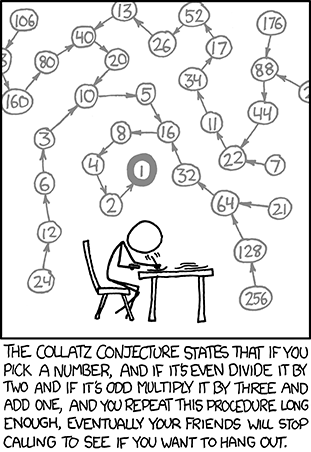
\includegraphics[height=2in]{prologue/pix/collatz_conjecture.png}  \\
  \caption{\href{https://xkcd.com/710/}{由 \texttt{xkcd.com} 提供}}
  \label{fig:XKCDCollatz}
\end{figure}
\end{exparts}
\end{answer}
\end{exercise}

\begin{exercise}
\begin{credit}
  SE user Ted, https://math.stackexchange.com/a/75300/12012 
\end{credit}
Ackermann 函数在直觉上是可机械计算的（并且是全函数），但它不是原始递归的。
下面给出另一个这样的函数。
% (It uses a technique from the next chapter called `diagonalization'.)
假设所有偏递归函数都接受一个自然数输入，并产生一个自然数输出。
（我们可以用 G\"{o}del 乘法编码模拟输入对等；参见\zcref{exer:CourseOfValuesRecursion}。）
令 $f_0$, $f_1$, \ldots{} 是所有原始递归函数的一个有效列表。
也就是说，存在一个原始递归函数，它输入索引~$i$，返回某种计算~$f_i$ 的方式。
（\textit{注：}~这相当于一个原始递归函数的解释器，给定函数的描述~$i$，就能对任意输入~$x$ 计算 $f_i(x)$。）
现在考虑函数$D(n)=f_n(n)+1$。
证明 $D$ 虽然直觉上可计算，但不是原始递归的。
\begin{answer}\verified
如果 $D$ 是原始递归的，那么它就是某个~$f_i$。
但这样一来$D(i)=f_i(i)+1=D(i)+1$，这是不可能的。  
\end{answer}
\end{exercise}

\end{exercises}
\index{general recursion|)}\index{recursion|)}

% ==================================
\extra{Turing 机模拟器}\index{Turing machine!simulator|(} \label{extra:TuringMachineSimilator}

本书的源代码仓库中包含一个用 Racket 编写的程序，用于模拟 Turing 机。
它位于目录
\lstinline{src/scheme/prologue}。
这里我们将展示如何运行这个模拟器。
（其实现紧密遵循
书中第~\pageref{DefnConfiguration}页对 Turing 机动作的描述。）

\zcref{ex:MPred}给出了一个计算
前驱函数的 Turing 机。
\begin{equation*}
 \TM_{\text{pred}}=
  \set{ \tminstruction{0}{B}{L}{1},\,
        \tminstruction{0}{1}{R}{0},\,
        \tminstruction{1}{B}{L}{2},\,
        \tminstruction{1}{1}{B}{1},\,
        \tminstruction{2}{B}{R}{3},\,
        \tminstruction{2}{1}{L}{2} 
      }
\end{equation*}
它对应于输入文件 \lstinline{pred.tm}。
\lstinputlisting{\tmfiles pred.tm}
因此，任何一个特定 Turing 机的模拟器实际上由两部分组成：
Racket 代码和机器的描述文件，如上所示。

下面是模拟器的一次运行，包括其命令行调用。
机器启动时的当前符号为 \str{1}，
当前符号右侧的纸带内容为 \str{11}（左侧的纸带为空）。
因此，整个纸带输入是 $\tau=\str{111}$。
因为 $3$ 的前驱是~$2$，我们期望结束时纸带会包含 \str{11}，其余部分为空白。
\begin{lstlisting} 
computing/src/scheme/prologue$ ./turing-machine.rkt -f machines/pred.tm -c "1" -r "11"
step 0: q0: *1*11
step 1: q0: 1*1*1
step 2: q0: 11*1*
step 3: q0: 111*B*
step 4: q1: 11*1*B
step 5: q1: 11*B*B
step 6: q2: 1*1*BB
step 7: q2: *1*1BB
step 8: q2: *B*11BB
step 9: q3: B*1*1BB
step 10: HALT
\end{lstlisting}  % $
输出虽然粗陋，但对于小实验来说已经足够。
命令行 \lstinline{turing-machine.rkt --help} 可以查看
模拟器的选项。

\begin{exercises}


\begin{exercise}
使用模拟器运行 $\TM_{\text{pred}}$，初始输入为 \str{11111}。
同时也以空纸带启动。
\begin{answer}
以下是以五个 \str{1} 作为初始输入的命令行运行记录。
\begin{lstlisting}
$ ./turing-machine.rkt -f machines/pred.tm -c "1" -r "1111"
step 0: q0: *1*1111
step 1: q0: 1*1*111
step 2: q0: 11*1*11
step 3: q0: 111*1*1
step 4: q0: 1111*1*
step 5: q0: 11111*B*
step 6: q1: 1111*1*B
step 7: q1: 1111*B*B
step 8: q2: 111*1*BB
step 9: q2: 11*1*1BB
step 10: q2: 1*1*11BB
step 11: q2: *1*111BB
step 12: q2: *B*1111BB
step 13: q3: B*1*111BB
step 14: HALT
\end{lstlisting}  % $
以下是其纸带图格式。
\begin{tapesequence}
  \begin{tapesequencetable}
    0 &\tapegraphic{\tmexercises pred_five000.pdf} \\
    1 &\tapegraphic{\tmexercises pred_five001.pdf} \\
    2 &\tapegraphic{\tmexercises pred_five002.pdf} \\
    3 &\tapegraphic{\tmexercises pred_five003.pdf} \\
    4 &\tapegraphic{\tmexercises pred_five004.pdf} \\
  \end{tapesequencetable}
  \hspace*{2em}
  \begin{tapesequencetable}
    5 &\tapegraphic{\tmexercises pred_five005.pdf} \\
    6 &\tapegraphic{\tmexercises pred_five006.pdf} \\
    7 &\tapegraphic{\tmexercises pred_five007.pdf} \\
    8 &\tapegraphic{\tmexercises pred_five008.pdf} \\
    9 &\tapegraphic{\tmexercises pred_five009.pdf} \\
  \end{tapesequencetable}
  \hspace*{2em}
  \begin{tapesequencetable}
   10 &\tapegraphic{\tmexercises pred_five010.pdf} \\
   11 &\tapegraphic{\tmexercises pred_five011.pdf} \\
   12 &\tapegraphic{\tmexercises pred_five012.pdf} \\
   13 &\tapegraphic{\tmexercises pred_five013.pdf} \\
  \end{tapesequencetable}
\end{tapesequence}
这是以空纸带作为初始输入的命令行调用，
\begin{lstlisting}
$ ./turing-machine.rkt -f machines/pred.tm -c " "
step 0: q0: *B*
step 1: q1: *B*B
step 2: q2: *B*BB
step 3: q3: B*B*B
step 4: HALT
\end{lstlisting}  % $
以及对应的纸带图序列。
\begin{tapesequence}
  \begin{tapesequencetable}
    0 &\tapegraphic{\tmexercises pred_empty000.pdf} \\
    1 &\tapegraphic{\tmexercises pred_empty001.pdf} \\
    2 &\tapegraphic{\tmexercises pred_empty002.pdf} \\
    3 &\tapegraphic{\tmexercises pred_empty003.pdf} \\
  \end{tapesequencetable}
\end{tapesequence}
\end{answer}
\end{exercise}

\begin{exercise}
在例~\ref{ex:MAdd}的加法 Turing 机 $\TM_{\text{add}}$ 上运行模拟器来计算 $1+2$。
同时模拟 $0+2$ 和 $0+0$。
\begin{answer}
这模拟了 $1+2$。
\begin{lstlisting}
$ ./turing-machine.rkt -f machines/pred.tm -c "1" -r " 11"
step 0: q0: *1* 11
step 1: q0: 1*B*11
step 2: q1: 1*B*11
step 3: q1: 1*1*11
step 4: q2: 1*1*11
step 5: q2: *1*111
step 6: q2: *B*1111
step 7: q3: *B*1111
step 8: q3: B*1*111
step 9: q4: B*B*111
step 10: q5: BB*1*11
step 11: HALT
\end{lstlisting}  % $
这是对应的纸带图。
\begin{tapesequence}
  \begin{tapesequencetable}
    0 &\tapegraphic{\tmexercises addonetwo000.pdf} \\
    1 &\tapegraphic{\tmexercises addonetwo001.pdf} \\
    2 &\tapegraphic{\tmexercises addonetwo002.pdf} \\
    3 &\tapegraphic{\tmexercises addonetwo003.pdf} \\
  \end{tapesequencetable}
  \hspace*{2em}
  \begin{tapesequencetable}
    4 &\tapegraphic{\tmexercises addonetwo004.pdf} \\
    5 &\tapegraphic{\tmexercises addonetwo005.pdf} \\
    6 &\tapegraphic{\tmexercises addonetwo006.pdf} \\
    7 &\tapegraphic{\tmexercises addonetwo007.pdf} \\
  \end{tapesequencetable}
  \hspace*{2em}
  \begin{tapesequencetable}
    8 &\tapegraphic{\tmexercises addonetwo008.pdf} \\
    9 &\tapegraphic{\tmexercises addonetwo009.pdf} \\
   10 &\tapegraphic{\tmexercises addonetwo010.pdf} \\
  \end{tapesequencetable}
\end{tapesequence}
$0+2$ 的命令行
\begin{lstlisting}
$ ./turing-machine.rkt -f machines/pred.tm -c " " -r "11"
\end{lstlisting}  % $
给出这些纸带图。
\begin{tapesequence}
  \begin{tapesequencetable}
    0 &\tapegraphic{\tmexercises addzerotwo000.pdf} \\
    1 &\tapegraphic{\tmexercises addzerotwo001.pdf} \\
    2 &\tapegraphic{\tmexercises addzerotwo002.pdf} \\
  \end{tapesequencetable}
  \hspace*{2em}
  \begin{tapesequencetable}
    3 &\tapegraphic{\tmexercises addzerotwo003.pdf} \\
    4 &\tapegraphic{\tmexercises addzerotwo004.pdf} \\
    5 &\tapegraphic{\tmexercises addzerotwo005.pdf} \\
  \end{tapesequencetable}
  \hspace*{2em}
  \begin{tapesequencetable}
    6 &\tapegraphic{\tmexercises addzerotwo006.pdf} \\
    7 &\tapegraphic{\tmexercises addzerotwo007.pdf} \\
    8 &\tapegraphic{\tmexercises addzerotwo008.pdf} \\
  \end{tapesequencetable}
\end{tapesequence}
$0+0$ 的命令行
\begin{lstlisting}
$ ./turing-machine.rkt -f machines/pred.tm -c " " 
\end{lstlisting}  % $
给出了以下纸带图序列。
\begin{tapesequence}
  \begin{tapesequencetable}
    0 &\tapegraphic{\tmexercises addzerozero000.pdf} \\
    1 &\tapegraphic{\tmexercises addzerozero001.pdf} \\
    2 &\tapegraphic{\tmexercises addzerozero002.pdf} \\
  \end{tapesequencetable}
  \hspace*{2em}
  \begin{tapesequencetable}
    3 &\tapegraphic{\tmexercises addzerozero003.pdf} \\
    4 &\tapegraphic{\tmexercises addzerozero004.pdf} \\
    5 &\tapegraphic{\tmexercises addzerozero005.pdf} \\
  \end{tapesequencetable}
  \hspace*{2em}
  \begin{tapesequencetable}
    6 &\tapegraphic{\tmexercises addzerozero006.pdf} \\
    7 &\tapegraphic{\tmexercises addzerozero007.pdf} \\
    8 &\tapegraphic{\tmexercises addzerozero008.pdf} \\
  \end{tapesequencetable}
\end{tapesequence}
\end{answer}
\end{exercise}

\begin{exercise}
编写一个 Turing 机来执行加~$3$ 的操作，
使得给定一个仅包含连续 $n$ 个 \str{1} 的串的纸带作为输入时，它返回一个包含连续 $n+3$ 个 \str{1} 的串的纸带。
遵循我们的约定：程序启动和结束时，读写头都位于第一个 \str{1} 的下方。
在模拟器上运行它，输入分别为 $4$ 个连续的 \str{1}，以及空纸带。
\begin{answer}
这个十条指令的机器
\begin{align*}
  \TM_{\text{addthree}} 
  &=
  \{\hspace{\setspacing} \tminstruction{0}{1}{R}{0},\,
        \tminstruction{0}{B}{B}{1},\,
        \tminstruction{1}{B}{1}{1},\,
        \tminstruction{1}{1}{R}{2},\,
        \tminstruction{2}{B}{1}{2},\,
        \tminstruction{2}{1}{R}{3},\,        \\
        &\qquad\;\tminstruction{3}{B}{1}{3},\,
        \tminstruction{3}{1}{1}{4},\,          
        \tminstruction{4}{1}{L}{4},\,
        \tminstruction{4}{B}{R}{5} 
      \hspace{\setspacing}\}
\end{align*}
\noindent 与模拟器的源文件一致。
\lstinputlisting{\tmfiles addthree.tm}
\noindent 输入为~$4$ 的命令行
\begin{lstlisting}
$ ./turing-machine.rkt -f machines/addthree.tm -c "1" -r "111"
\end{lstlisting}  % $
\noindent 给出了以下纸带图。
\begin{tapesequence}
  \begin{tapesequencetable}
    0  &\tapegraphic{\tmexercises addthree_four000.pdf} \\
    1  &\tapegraphic{\tmexercises addthree_four001.pdf} \\
    2  &\tapegraphic{\tmexercises addthree_four002.pdf} \\
    3  &\tapegraphic{\tmexercises addthree_four003.pdf} \\
    4  &\tapegraphic{\tmexercises addthree_four004.pdf} \\
    5  &\tapegraphic{\tmexercises addthree_four005.pdf} \\
    6  &\tapegraphic{\tmexercises addthree_four006.pdf} \\
  \end{tapesequencetable}
  \hspace*{2em}
  \begin{tapesequencetable}
    7  &\tapegraphic{\tmexercises addthree_four007.pdf} \\
    8  &\tapegraphic{\tmexercises addthree_four008.pdf} \\
    9  &\tapegraphic{\tmexercises addthree_four009.pdf} \\
   10  &\tapegraphic{\tmexercises addthree_four010.pdf} \\
   11  &\tapegraphic{\tmexercises addthree_four011.pdf} \\
   12  &\tapegraphic{\tmexercises addthree_four012.pdf} \\
   13  &\tapegraphic{\tmexercises addthree_four013.pdf} \\
  \end{tapesequencetable}
  \hspace*{2em}
  \begin{tapesequencetable}
   14  &\tapegraphic{\tmexercises addthree_four014.pdf} \\
   15  &\tapegraphic{\tmexercises addthree_four015.pdf} \\
   16  &\tapegraphic{\tmexercises addthree_four016.pdf} \\
   17  &\tapegraphic{\tmexercises addthree_four017.pdf} \\
   18  &\tapegraphic{\tmexercises addthree_four018.pdf} \\
   19  &\tapegraphic{\tmexercises addthree_four019.pdf} \\
  \end{tapesequencetable}
\end{tapesequence}
输入为 $0$ 的命令行
\begin{lstlisting}
$ ./turing-machine.rkt -f machines/addthree.tm -c " " 
\end{lstlisting}  % $
\noindent 给出了以下纸带图序列。
\begin{tapesequence}
  \begin{tapesequencetable}
    0  &\tapegraphic{\tmexercises addthree_zero000.pdf} \\
    1  &\tapegraphic{\tmexercises addthree_zero001.pdf} \\
    2  &\tapegraphic{\tmexercises addthree_zero002.pdf} \\
    3  &\tapegraphic{\tmexercises addthree_zero003.pdf} \\
  \end{tapesequencetable}
  \hspace*{2em}
  \begin{tapesequencetable}
    4  &\tapegraphic{\tmexercises addthree_zero004.pdf} \\
    5  &\tapegraphic{\tmexercises addthree_zero005.pdf} \\
    6  &\tapegraphic{\tmexercises addthree_zero006.pdf} \\
    7  &\tapegraphic{\tmexercises addthree_zero007.pdf} \\
  \end{tapesequencetable}
  \hspace*{2em}
  \begin{tapesequencetable}
    8  &\tapegraphic{\tmexercises addthree_zero008.pdf} \\
    9  &\tapegraphic{\tmexercises addthree_zero009.pdf} \\
   10  &\tapegraphic{\tmexercises addthree_zero010.pdf} \\
   11  &\tapegraphic{\tmexercises addthree_zero011.pdf} \\
  \end{tapesequencetable}
\end{tapesequence}
\end{answer}
\end{exercise}

\begin{exercise}
编写一台机器来判定输入是否包含子串~\str{010}。
固定 $\Sigma=\set{\str{0}, \str{1}, \str{B}}$。
机器初始时，纸带上除了一串连续的 \str{0} 和 \str{1} 外全是空白，
且读写头位于第一个非空白符号下方。
结束时，如果输入包含所需的子串，则纸带上将只有一个~\str{1}；
否则只有一个~\str{0}。
我们将分阶段进行，构建几个相当于子程序的部分。
\begin{exparts}
\item 编写从状态~$q_{10}$ 开始的指令，使得如果初始时机器的读写头位于一串非空白符号的首个上方，那么结束时读写头将处于最后一个此类符号的右侧。
\item 编写从状态~$q_{20}$ 开始的一系列指令，使得如果初始时读写头紧邻一串非空白符号的右侧，那么结束时所有这些符号都变为空白。
\item 编写完整的机器，包括将前面的项连接起来。
\end{exparts}
\begin{answer}
\begin{exparts}
\item
像下面这样就可以了。
\begin{equation*}
  \TM_0=\set{\tminstruction{10}{0}{R}{10},\,
       \tminstruction{10}{1}{R}{10},\,
       \tminstruction{10}{B}{B}{100} }
\end{equation*}
\item
这会向后移动，将格子擦除为空白。
\begin{equation*}
  \TM_1=\set{ 
       \tminstruction{20}{0}{B}{21},\,
       \tminstruction{20}{1}{B}{21},\,
       \tminstruction{20}{B}{B}{100},\,   
       \tminstruction{21}{0}{L}{20},\,
       \tminstruction{21}{1}{L}{20},\,
       \tminstruction{21}{B}{L}{20} 
      }
\end{equation*}
\item 这里，粗略地说，$q_0$ 表示尚未匹配到子串的任何部分，
$q_1$ 表示已看到 \str{0}，机器正在寻找~\str{1}，
而~$q_2$ 表示已看到 \str{01}，机器正在寻找~\str{0}。
接着，四个状态 $q_3$、$q_4$、$q_5$ 和 $q_6$ 表示失败
（它们以 $q_6$ 在空白纸带上写入~\str{0} 而结束）。
四个状态 $q_7$、$q_8$、$q_9$ 和 $q_{10}$ 表示成功。
\begin{align*}
  \TM_{\text{decide010}} 
  &=
  \{\hspace{\setspacing} \tminstruction{0}{0}{R}{1},\,
        \tminstruction{0}{1}{R}{0},\,
        \tminstruction{0}{B}{B}{3},\,
        \tminstruction{1}{0}{R}{1},\,
        \tminstruction{1}{1}{R}{2},\,
        \tminstruction{1}{B}{B}{3},\,        
        \tminstruction{2}{0}{R}{7},\,
        \tminstruction{2}{1}{1}{0},\,
        \tminstruction{2}{B}{B}{3},\,        \\
        &\qquad\;
        \tminstruction{3}{0}{R}{3},\,
        \tminstruction{3}{1}{R}{3},\,          
        \tminstruction{3}{B}{L}{4},\,
        \tminstruction{4}{0}{B}{5},\,
        \tminstruction{4}{1}{B}{5},\,       
        \tminstruction{4}{B}{B}{6},\,   \\  % too big to fit on one line
        &\qquad\qquad\tminstruction{5}{0}{L}{4},\,
        \tminstruction{5}{1}{L}{4},\,          
        \tminstruction{5}{B}{L}{4},\,
        \tminstruction{6}{0}{0}{100},\,
        \tminstruction{6}{1}{0}{100},\,          
        \tminstruction{6}{B}{0}{100},\,      \\
        &\qquad\;
        \tminstruction{7}{0}{R}{7},\,
        \tminstruction{7}{1}{R}{7},\,          
        \tminstruction{7}{B}{L}{8},\,
        \tminstruction{8}{0}{B}{9},\,
        \tminstruction{8}{1}{B}{9},\,          
        \tminstruction{8}{B}{B}{10},\,      \\  % too big
        &\qquad\qquad\tminstruction{9}{0}{L}{8},\,
        \tminstruction{9}{1}{L}{8},\,          
        \tminstruction{9}{B}{L}{8},\,
        \tminstruction{10}{0}{1}{100},\,
        \tminstruction{10}{1}{1}{100},\,          
        \tminstruction{10}{B}{1}{100}      
      \hspace{\setspacing}\}
\end{align*}
\end{exparts}
\end{answer}
\end{exercise}

% Write a Turing machine to perform the proper subtraction
% operation on two inputs, often denoted $x\dotminus y$,
% that yields $x-y$ if $x\geq y$ and~$0$ otherwise. 
% Run it on the simulator to compute $5\dotminus 3$ and $3\dotminus 5$.

% \begin{exercise}
% Modify the simulator so that it can run for a limited number of steps.
% \begin{exparts}
% \item Modify it so that, given~$k\in\N$, if the Turing machine hasn't halted
% after $k$ steps then the simulator stops.
% \item Do the same, but replace $k$ with a function \codeinline{(k n)} where
% \str{n} is the input number (assume the machine's input is a string
% of \str{1}'s). 
% \end{exparts}
% \end{exercise}

\end{exercises}
\index{Turing machine!simulator|)}

% ==================================
\extra{硬件}  \label{extra:Hardware}
遵循 Turing 的方法，我们已经基于转移构建了关于“什么是可计算的”的定义。
我们生成一个转移指令表，并将其称为一台机器。
但是，我们能否确定每个转移表都有一个对应的实际机制，
即一个具有该行为的物理实现呢？

换个说法，在编程语言中，存在由其他更简单的运算符构造而成的运算符。
例如，\citetext{$\sin(x)$ 可以通过其 Taylor 多项式计算}{%
  Taylor 级数是 $\sin(x)=x-x^3/3!+x^5/5!-x^7/7!+\cdots$。
  我们可以通过决定在 $x^5$ 项截断该级数来得到一个 Taylor 多项式，从而进行实际计算。} 的值可由加法和乘法计算得出。
但是，最基本的操作必须在硬件层面发生；它们是如何实现的呢？

我们将展示如何从任何期望的行为出发，构造出相应的设备。
为此，我们将处理以比特串作为输入和输出的机器。
最简单的方法是通过命题逻辑。
（\zcref{sec:PropLogic}处有相关回顾。）

以下是三个基本的逻辑运算符。
这些表格用 $0$ 替代~$F$，用 $1$ 替代~$T\!$，这是电子学中的惯例。


\begin{center}\small % \vspace{0.5ex}
  \begin{tabular}[t]{c|c}
    \multicolumn{1}{c}{\ }    
        &\multicolumn{1}{c}{\tabulartext{非}$P$}  \\[-0.25ex]
    \multicolumn{1}{c}{$P$}      
        &\multicolumn{1}{c}{$\neg P$}  \\
    \hline
       $0$  &$1$  \\
       $1$  &$0$
  \end{tabular}
  \qquad
  \begin{tabular}[t]{cc|cc}
    \multicolumn{1}{c}{\ }    
        &\multicolumn{1}{c}{\ }    
        &\multicolumn{1}{c}{$P$ \tabulartext{与} $Q$}  
        &\multicolumn{1}{c}{$P$ \tabulartext{或} $Q$}  \\[-0.25ex]
    \multicolumn{1}{c}{$P$}      
        &\multicolumn{1}{c}{$Q$}      
        &\multicolumn{1}{c}{$P\wedge Q$}  
        &\multicolumn{1}{c}{$P\vee Q$}  \\
    \hline
       $0$  &$0$  &$0$  &$0$  \\
       $0$  &$1$  &$0$  &$1$  \\
       $1$  &$0$  &$0$  &$1$  \\
       $1$  &$1$  &$1$  &$1$  
  \end{tabular}
\end{center}

这三个逻辑运算符就是我们所需的全部。
我们将展示如何从一个指定的输入-输出行为，即一个期望的真值表，
得到一个仅使用“$\neg$”、“$\wedge$”和“$\vee$”并具有该行为的命题逻辑表达式。
然后我们将概述如何用电子元件实现它。

下面的两个表格展示了具体做法。
从左边那个表格开始，关注输出为~$1$ 的那一行。
表达式 $\neg P\wedge \neg Q$
使这一行的值为~$1$，而其他所有行的值为~$0$。


\begin{center} \small
  \begin{tabular}[t]{cc|c}
    \multicolumn{1}{c}{$P$}      
        &\multicolumn{1}{c}{$Q$}      
        &\multicolumn{1}{c}{}  \\
    \hline
       $0$  &$0$  &$1$  \\
       $0$  &$1$  &$0$  \\
       $1$  &$0$  &$0$  \\
       $1$  &$1$  &$0$  
  \end{tabular}
  \hspace{3em}
  \begin{tabular}[t]{ccc|c}
    \multicolumn{1}{c}{$P$}
    &\multicolumn{1}{c}{$Q$}
    &\multicolumn{1}{c}{$R$}
    &\multicolumn{1}{c}{}     \\ \hline
    $0$  &$0$  &$0$  &$0$    \\
    $0$  &$0$  &$1$  &$1$    \\
    $0$  &$1$  &$0$  &$1$    \\
    $0$  &$1$  &$1$  &$0$    \\[.5ex]
    $1$  &$0$  &$0$  &$1$    \\
    $1$  &$0$  &$1$  &$0$    \\
    $1$  &$1$  &$0$  &$0$    \\
    $1$  &$1$  &$1$  &$0$    
  \end{tabular}  
\end{center}


对于右边的表格，同样关注输出为~$1$ 的那些行。
第二行对应的子句是 $\neg P\wedge \neg Q\wedge R$。
针对第三行，使用 $\neg P\wedge Q\wedge \neg R$；
针对第五行，使用 $P\wedge\neg Q\wedge\neg R$。
现在用 $\vee$ 将这些子句组合起来，就得到了符合给定真值表的命题。
（由使用 $\wedge$ 的子句并通过 $\vee$ 连接而成的命题，称为析取范式（DNF）。
参见\zcref{sec:PropLogic}。）\index{Disjunctive Normal form, DNF}\index{DNF}\index{Propositional logic!Disjunctive Normal form}
\begin{equation*}
(\neg P\wedge \neg Q\wedge R)
  \vee(\neg P\wedge Q\wedge \neg R)
  \vee(P\wedge\neg Q\wedge\neg R)
\tag{$*$}
\end{equation*}

\margingraphic{0.22\textwidth}{prologue/pix/shannon.jpg}{\label{fig:shannon}\href{https://en.wikipedia.org/wiki/Claude_Shannon}{Claude Shannon 1916--2001}}\index{Shannon, C!picture}
% See also http://nautil.us/issue/51/limits/how-information-got-re_invented
接下来，我们将这些表达式转化为器件。
利用这种形式的命题逻辑表达式来系统地设计逻辑电路，这一发现是由\citetext{C~Shannon}{参见他的个人简介：\protect\url{http://www.newyorker.com/tech/elements/claude-shannon-the-father-of-the-information-age-turns-1100100}.} 在其 1937 年的\citetext{硕士论文}{%
他的相关论文就是他的硕士论文，\protect\url{https://en.wikipedia.org/wiki/A_Symbolic_Analysis_of_Relay_and_Switching_Circuits}.} 中提出的。
我们可以获得被称为
\definend{门}的电子器件，\index{gate}\index{logic gate}
它能对信号执行逻辑操作。
（在本讨论中，我们将出现 $5$ 伏特电压视为信号 $1$，$0$ 伏特视为信号 $0$）。
下方左侧是一个具有两根输入导线和一根输出导线的
\textsc{与}门的电路符号，其行为是：只有当两个输入端都有信号时，输出端才会有信号。
中间所画的是一个 \textsc{或}门的符号，只要任一输入端有信号，输出端就有信号。
右侧是一个 \textsc{非}门的符号。


\begin{center}
  \vcenteredhbox{\includegraphics{prologue/asy/gates/gates00.pdf}}
  \qquad
  \vcenteredhbox{\includegraphics{prologue/asy/gates/gates01.pdf}}
  \qquad
  \vcenteredhbox{\includegraphics{prologue/asy/gates/gates02.pdf}}
\end{center}

下方给出了实现表达式~($*$) 的电路示意图，左侧的三条导线表示三个输入信号。
例如，为了实现第一个子句，顶部的 \textsc{与}门接收非~$P$、非~$Q$ 和~$R$ 信号。
第二和第三个子句由另外两个 \textsc{与}门实现。
然后，\textsc{与}门的输出被送入 \textsc{或}门。
（这些 \textsc{与}门和 \textsc{或}门被设计为能接收三个输入；我们不必在意市面上实际出售的是哪些类型的这种器件。）


\begin{center}
  \includegraphics{prologue/asy/gates/gates03.pdf}
\end{center}

显然，遵循这一步骤，我们原则上可以构建出具有任何期望输入/输出行为的物理设备。
特别地，我们可以通过这种方式构建一台 Turing 机。

最后，我们稍作题外探讨。
有人可能会好奇这些门是如何构造的，特别是会好奇一个 \textsc{非}门怎么可能存在——输入端没有电压时输出端却有电压，这不是无中生有吗？

答案是，上述描述抽象掉了一些细节。
这里展示了一种
\citetext{\textsc{非}门}{%
这是 N 型金属氧化物半导体晶体管的一种。还有许多其他类型。}
的内部构造。


\begin{center}
  \includegraphics{prologue/asy/gates/gates04.pdf}
\end{center}


右边是一个电池，正如我们将要看到的，它提供了额外的电压。
左上角画成波浪线的是电阻。当电流流经电路时，该电阻会调节来自电池的功率输出。

左下角带有圆圈的是晶体管。如果在~\textsf{G} 和~\textsf{S} 之间有足够的电压，该元件就会允许来自电池的电流在 \textsf{D} 和 \textsf{S} 之间流动。
（因为它有时断开有时闭合，所以被画作开关，尽管它并没有活动部件。）
这种晶体管在制造时设定为，$5$ 伏特的输入电压~$V_{\text{in}}$ 即可触发这一动作。

为了验证该电路对信号取反，首先假设 $V_{\text{in}}=0$。
那么，\textsf{D} 和~\textsf{S} 之间没有电流流动。
由于没有电流，电阻不会产生电压降，因此间隙两端的输出电压~$V_{\text{out}}$ 等于电池提供的全部电压，即 $5$ 伏特。
所以，$V_{\text{in}}=0$ 使得~$V_{\text{out}}=5$。

反之，假设 $V_{\text{in}}=5$。
那么电流在 \textsf{D} 和~\textsf{S} 之间流动，电阻因此产生电压降，这意味着输出为~$V_{\text{out}}=0$。

因此，对于这个器件，输出电压 $V_{\text{out}}$ 与输入电压~$V_{\text{in}}$ 相反。
% When $V_{\text{in}}=0$ the output voltage of~$5$ doesn't come from 
% nowhere;~it comes from the battery.

\begin{exercises}

\begin{exercise}
一个常用的命题逻辑运算符是
\definend{异或（\textsc{XOR}）}。\index{exclusive or@exclusive or \textsc{XOR}}\index{XOR@\textsc{XOR}, exclusive or}\index{Propositional logic!exclusive or@exclusive or \textsc{XOR}}
其定义为：$P\mathbin{\textsc{XOR}}Q=1$ 为 $1$ 当且仅当 $P\neq Q$。
\begin{exparts}
\item 列出真值表，并根据它构造一个析取范式（DNF）命题逻辑表达式。
\item 用该表达式设计一个回路。
\end{exparts}
\begin{answer}\verified
\begin{exparts}
\item 真值表如下。
\begin{display}
  \begin{tabular}[t]{cc|c}
    \multicolumn{1}{c}{$P$}      
        &\multicolumn{1}{c}{$Q$}      
        &\multicolumn{1}{c}{$P\mathbin{\textsc{XOR}}Q$}  \\
    \hline
       $0$  &$0$  &$0$  \\
       $0$  &$1$  &$1$  \\
       $1$  &$0$  &$1$  \\
       $1$  &$1$  &$0$  
  \end{tabular}    
\end{display}
表达式为$(\neg P\wedge \neg Q)
  \vee(P\wedge Q)$。
\item  $P\mathbin{\textsc{XOR}}Q$ 的回路如图\figureref{fig:PxorQCircuit}所示。
\begin{figure} 
  \centering
  \includegraphics{prologue/asy/gates/gates06.pdf}  \\
  \caption{$P\mathbin{\textsc{XOR}}Q$ 的回路。}
  \label{fig:PxorQCircuit}
\end{figure}
\end{exparts}
\end{answer}
\end{exercise}

\begin{exercise}
命题逻辑运算符
\definend{蕴含}（\definend{$\rightarrow$}）\index{Propositional logic!implication}\index{implication logic operator $\rightarrow$}
定义为：除了 $P$ 为 $1$ 且 $Q$ 为 $0$ 的情况外，$P\rightarrow Q$ 均为 $1$。
\begin{exparts}
\item 列出真值表，并根据它构造一个析取范式表达式。
\item 用该表达式设计一个回路。
\end{exparts}
\begin{answer}\verified
\begin{exparts}
\item 根据定义，输入/输出行为如下：
\begin{display} \small
  \begin{tabular}[t]{cc|c}
    \multicolumn{1}{c}{$P$}
    &\multicolumn{1}{c}{$Q$}
    &\multicolumn{1}{c}{$P\rightarrow Q$}     \\ \hline
    $0$  &$0$  &$1$    \\
    $0$  &$1$  &$1$    \\
    $1$  &$0$  &$0$    \\
    $1$  &$1$  &$1$    
  \end{tabular}  
\end{display}
因此，布尔表达式为
$(\neg P\wedge \neg Q)
  \vee(\neg P\wedge Q)
  \vee(P\wedge Q)$。
\item 蕴含运算的回路如图\figureref{fig:ImpliesCircuit}所示。
\begin{figure} 
  \centering
  \includegraphics{prologue/asy/gates/gates11.pdf}  \\
  \caption{蕴含运算的回路。}
  \label{fig:ImpliesCircuit}
\end{figure}
\end{exparts}
\end{answer}
\end{exercise}

\begin{exercise}
根据下表构造一个析取范式命题逻辑表达式。
\begin{center} \small
  \begin{tabular}[t]{cc|c}
    \multicolumn{1}{c}{$P$}
    &\multicolumn{1}{c}{$Q$}
    &\multicolumn{1}{c}{}     \\ \hline
    $0$  &$0$  &$0$    \\
    $0$  &$1$  &$1$    \\
    $1$  &$0$  &$0$    \\
    $1$  &$1$  &$1$    
  \end{tabular}  
\end{center}
用该表达式设计一个回路。
\begin{answer}\verified
表达式为$(\neg P\wedge Q)
  \vee(P\wedge Q)$。
回路如图\figureref{fig:QCircuit}所示。
\begin{figure} 
  \centering
  \includegraphics{prologue/asy/gates/gates08.pdf}  \\
  \caption{未命名运算的回路（不妨称之为 $Q$）。}
  \label{fig:QCircuit}
\end{figure}
\end{answer}
\end{exercise}

\begin{exercise}
为下表各构造一个析取范式命题逻辑表达式。
\begin{center} \small
  \begin{tabular}[t]{ccc|c}
    \multicolumn{1}{c}{$P$}
    &\multicolumn{1}{c}{$Q$}
    &\multicolumn{1}{c}{$R$}
    &\multicolumn{1}{c}{}     \\ \hline
    $0$  &$0$  &$0$  &$0$    \\
    $0$  &$0$  &$1$  &$1$    \\
    $0$  &$1$  &$0$  &$1$    \\
    $0$  &$1$  &$1$  &$0$    \\[.5ex]
    $1$  &$0$  &$0$  &$0$    \\
    $1$  &$0$  &$1$  &$1$    \\
    $1$  &$1$  &$0$  &$0$    \\
    $1$  &$1$  &$1$  &$0$    
  \end{tabular}  
  \qquad
  \begin{tabular}[t]{ccc|c}
    \multicolumn{1}{c}{$P$}
    &\multicolumn{1}{c}{$Q$}
    &\multicolumn{1}{c}{$R$}
    &\multicolumn{1}{c}{}     \\ \hline
    $0$  &$0$  &$0$  &$1$    \\
    $0$  &$0$  &$1$  &$0$    \\
    $0$  &$1$  &$0$  &$1$    \\
    $0$  &$1$  &$1$  &$0$    \\[.5ex]
    $1$  &$0$  &$0$  &$0$    \\
    $1$  &$0$  &$1$  &$0$    \\
    $1$  &$1$  &$0$  &$1$    \\
    $1$  &$1$  &$1$  &$1$    
  \end{tabular}  
\end{center}
用这些表达式设计回路：
\begin{exparts}
\item 左表；
\item 右表。
\end{exparts}
\begin{answer}\verified
两个回路如图\figureref{fig:BothTableCircuits}所示。
\begin{figure} 
  \centering
  \vcenteredhbox{\includegraphics{prologue/asy/gates/gates09.pdf}}  
  \qquad
  \vcenteredhbox{\includegraphics{prologue/asy/gates/gates10.pdf}}  \\
  \caption{两个未命名运算表的回路。}
  \label{fig:BothTableCircuits}
\end{figure}
\begin{exparts}
\item 在表达式中，每个子句对应输出为 $1$ 的一行。
\begin{equation*}
(\neg P\wedge \neg Q\wedge R)
  \vee(\neg P\wedge Q\wedge \neg R)
  \vee(P\wedge \neg Q\wedge R)
\end{equation*}
\item 子句对应输出为 $1$ 的行。
\begin{equation*}
(\neg P\wedge \neg Q\wedge \neg R)
  \vee(\neg P\wedge Q\wedge \neg R)
  \vee(P\wedge Q\wedge \neg R)
  \vee(P\wedge Q\wedge R).
\end{equation*}
\end{exparts}
\end{answer}
\end{exercise}

\begin{exercise}
针对“若 $P$ 等于 $R$ 则输出为 $1$”的行为，制作一个以 $P$、$Q$ 和 $R$ 为输入的真值表。
写出对应的析取范式（DNF）表达式。
画出回路图。
\begin{answer}\verified
输入/输出行为如下：
\begin{display}
  \begin{tabular}[t]{ccc|c}
    \multicolumn{1}{c}{$P$}
    &\multicolumn{1}{c}{$Q$}
    &\multicolumn{1}{c}{$R$}
    &\multicolumn{1}{c}{}     \\ \hline
    $0$  &$0$  &$0$  &$1$    \\
    $0$  &$0$  &$1$  &$0$    \\
    $0$  &$1$  &$0$  &$1$    \\
    $0$  &$1$  &$1$  &$0$    \\[.5ex]
    $1$  &$0$  &$0$  &$0$    \\
    $1$  &$0$  &$1$  &$1$    \\
    $1$  &$1$  &$0$  &$0$    \\
    $1$  &$1$  &$1$  &$1$    
  \end{tabular}  
\end{display}
该表直接给出了析取范式（DNF）表达式：
\begin{equation*}
(\neg P\wedge \neg Q\wedge \neg R)
  \vee(\neg P\wedge Q\wedge \neg R)
  \vee(P\wedge\neg Q\wedge R)
  \vee(P\wedge Q\wedge R)
\end{equation*}
回路如图\figureref{fig:PEqualsRCircuit}所示。
\begin{figure} 
  \centering
  \includegraphics{prologue/asy/gates/gates05.pdf}  \\
  \caption{$P=R$ 的回路。}
  \label{fig:PEqualsRCircuit}
\end{figure}
\end{answer}
\end{exercise}

\begin{exercise}
针对“多数输入为 $1$ 时输出为 $1$”的行为，制作一个三输入真值表。
写出对应的析取范式（DNF）表达式。
画出回路图。
\begin{answer}\verified
当且仅当有两个或三个输入为 $1$ 时，该行的输出列才为 $1$。
\begin{display}
  \begin{tabular}[t]{ccc|c}
    \multicolumn{1}{c}{$P$}
    &\multicolumn{1}{c}{$Q$}
    &\multicolumn{1}{c}{$R$}
    &\multicolumn{1}{c}{}     \\ \hline
    $0$  &$0$  &$0$  &$0$    \\
    $0$  &$0$  &$1$  &$0$    \\
    $0$  &$1$  &$0$  &$0$    \\
    $0$  &$1$  &$1$  &$1$    \\[.5ex]
    $1$  &$0$  &$0$  &$0$    \\
    $1$  &$0$  &$1$  &$1$    \\
    $1$  &$1$  &$0$  &$1$    \\
    $1$  &$1$  &$1$  &$1$    
  \end{tabular}  
\end{display}
这是一个析取范式（DNF）表达式：
\begin{equation*}
(\neg P\wedge Q\wedge R)
  \vee(P\wedge \neg Q\wedge R)
  \vee(P\wedge Q\wedge \neg R)
  \vee(P\wedge Q\wedge R)
\end{equation*}
回路如图\figureref{fig:MajorityInputsCircuit}所示。
\begin{figure} 
  \centering
  \includegraphics{prologue/asy/gates/gates07.pdf}  \\
  \caption{三输入多数运算符的回路。}
  \label{fig:MajorityInputsCircuit}
\end{figure}
\end{answer}
\end{exercise}

\begin{exercise}
考虑如下输入/输出行为：多数输入为 $1$ 时输出为 $1$（不允许平局）。
\begin{exparts}
\item 针对此行为制作一个四输入真值表。
写出对应的析取范式（DNF）表达式。
\item 
同时写出此行为在五输入下的 DNF 表达式。
\end{exparts}
\begin{answer}\verified
\begin{exparts}
\item 当且仅当有三个或四个输入为 $1$ 时，该行的输出列才为 $1$。
\begin{display}
  \begin{tabular}[t]{cccc|c}
    \multicolumn{1}{c}{$P$}
    &\multicolumn{1}{c}{$Q$}
    &\multicolumn{1}{c}{$R$}
    &\multicolumn{1}{c}{$S$}
    &\multicolumn{1}{c}{}     \\ \hline
    $0$  &$0$  &$0$  &$0$  &$0$    \\
    $0$  &$0$  &$0$  &$1$  &$0$    \\
    $0$  &$0$  &$1$  &$0$  &$0$    \\
    $0$  &$0$  &$1$  &$1$  &$0$    \\[.5ex]
    $0$  &$1$  &$0$  &$0$  &$0$    \\
    $0$  &$1$  &$0$  &$1$  &$0$    \\
    $0$  &$1$  &$1$  &$0$  &$0$    \\
    $0$  &$1$  &$1$  &$1$  &$1$    \\[.5ex]
    $1$  &$0$  &$0$  &$0$  &$0$    \\
    $1$  &$0$  &$0$  &$1$  &$0$    \\
    $1$  &$0$  &$1$  &$0$  &$0$    \\
    $1$  &$0$  &$1$  &$1$  &$1$    \\[.5ex]
    $1$  &$1$  &$0$  &$0$  &$0$    \\
    $1$  &$1$  &$0$  &$1$  &$1$    \\
    $1$  &$1$  &$1$  &$0$  &$1$    \\
    $1$  &$1$  &$1$  &$1$  &$1$    \\
  \end{tabular}  
\end{display}
此 DNF 表达式包含所有至少有三个变量未被否定的子句。
\begin{equation*}
(\neg P\wedge Q\wedge R\wedge S)
  \vee(P\wedge \neg Q\wedge R\wedge S)
  \vee(P\wedge Q\wedge \neg R\wedge S)
  \vee(P\wedge Q\wedge R\wedge \neg S)
  \vee(P\wedge Q\wedge R\wedge S)
\end{equation*}
\item DNF 表达式必须由至少有三个变量未被否定的子句构成。
其中，恰好有三个未被否定的变量的子句有 $\binom{5}{3}=10$ 个，
恰好有一个被否定的变量（即四个未被否定的变量）的子句有 $\binom{5}{4}=5$ 个，
没有变量被否定的子句有 $\binom{5}{5}=1$ 个。
\begin{align*}
&(\neg P\wedge \neg Q\wedge R\wedge S\wedge T)
 \vee (\neg P\wedge Q\wedge \neg R\wedge S\wedge T)
 \vee (\neg P\wedge Q\wedge R\wedge \neg S\wedge T)
 \vee (\neg P\wedge Q\wedge R\wedge S\wedge \neg T)  \\
 &\quad\vee (P\wedge \neg Q\wedge \neg R\wedge S\wedge T)
 \vee (P\wedge \neg Q\wedge R\wedge \neg S\wedge T)
 \vee (P\wedge \neg Q\wedge R\wedge S\wedge \neg T)  \\
 &\quad\vee (P\wedge Q\wedge \neg R\wedge \neg S\wedge T)
 \vee (P\wedge Q\wedge \neg R\wedge S\wedge \neg T)
 \vee (P\wedge Q\wedge R\wedge \neg S\wedge \neg T)  \\
 &\vee (\neg P\wedge Q\wedge R\wedge S\wedge T)
 \vee (P\wedge \neg Q\wedge R\wedge S\wedge T)
 \vee (P\wedge Q\wedge \neg R\wedge S\wedge T)  \\
 &\quad\vee (P\wedge Q\wedge R\wedge \neg S\wedge T)
 \vee (P\wedge Q\wedge R\wedge S\wedge \neg T)  \\
 &\vee (P\wedge Q\wedge R\wedge S\wedge T)
\end{align*}
\end{exparts}
\end{answer}
\end{exercise}

\begin{exercise}
将两个二进制数相加，最自然的方法就像小学的十进制加法算法那样。
从最右边的个位列开始。
将这两个比特相加，并可能向下一列进位~$1$。
然后向下计算下一列，并包含任何进位。
从右到左重复这一过程。
\begin{exparts}
\item 用这个方法计算二进制数 $1011$ 和 $1001$ 的和。
\item 制作一个真值表，描述单列加法应有的行为。
  因为有进位的可能，它必须有三个输入。
  它还必须有两个输出列，一列是和的最低有效位，另一列是产生的进位（如果有的话）。
\item 画出对应的电路。
\end{exparts}
\begin{answer}\verified
\begin{exparts}
\item 计算过程如下表所示。
进位出现在从右数的第二、第三和第五列。
\begin{equation*}
  \begin{array}{*{5}{r}}
  {}^1 &1   &{}^10  &{^1}1  &1  \\
  +    &1   &0      &0      &1  \\ \cline{1-5}
  1    &0   &1      &0      &0  \\
  \end{array}
\end{equation*}
\item 定义给出了以下两个输入/输出行为。
这里所谓的“最低有效位”通常被称为“全加器”。
（也常用的是“半加器”，它不考虑进位输入，因此只有两个输入。）
\begin{display} \small
  \begin{tabular}[t]{ccc|cc}
    \multicolumn{1}{c}{进位输入 $I$}
    &\multicolumn{1}{c}{$P$}
    &\multicolumn{1}{c}{$Q$}
    &\multicolumn{1}{c}{\text{最低有效位 $L$}}
    &\multicolumn{1}{c}{\text{进位输出 $C$}}     \\ \hline
    $0$  &$0$  &$0$  &$0$ &$0$    \\
    $0$  &$0$  &$1$  &$1$ &$0$    \\
    $0$  &$1$  &$0$  &$1$ &$0$    \\
    $0$  &$1$  &$1$  &$0$ &$1$    \\[0.5ex]
    $1$  &$0$  &$0$  &$1$ &$0$    \\
    $1$  &$0$  &$1$  &$0$ &$1$    \\
    $1$  &$1$  &$0$  &$0$ &$1$    \\
    $1$  &$1$  &$1$  &$1$ &$1$    \\[0.5ex]
  \end{tabular}  
\end{display}
对于~$L$，一个布尔表达式是  
$(\neg I\wedge \neg P\wedge Q)
  \vee(\neg I\wedge P\wedge \neg Q)
  \vee(I\wedge \neg P\wedge \neg Q)
  \vee(I\wedge P\wedge Q)$。
对于~$C$，一个析取范式（DNF）表达式是   
$(\neg I\wedge P\wedge Q)
  \vee(I\wedge \neg P\wedge Q)
  \vee(I\wedge P\wedge \neg Q)
  \vee(I\wedge P\wedge Q)$。
\item 图\figureref{fig:AdderCircuits}给出了对应的电路。
\begin{figure} 
  \centering
  \vcenteredhbox{\includegraphics{prologue/asy/gates/gates12.pdf}}  
  \qquad
  \vcenteredhbox{\includegraphics{prologue/asy/gates/gates13.pdf}}  \\
  \caption{单列加法的部分和与进位电路。}
  \label{fig:AdderCircuits}
\end{figure}
\end{exparts}
\end{answer}
\end{exercise}

% \begin{exercise}
% Construct a circuit with the behavior specified in the tables below:
% \begin{exparts*}
% \item the table on the left,
% \item the one on the right.
% \end{exparts*}
% \begin{center} \small
%   \begin{tabular}[t]{ccc|c}
%     \multicolumn{1}{c}{$P$}
%     &\multicolumn{1}{c}{$Q$}
%     &\multicolumn{1}{c}{$R$}
%     &\multicolumn{1}{c}{}     \\ \hline
%     $0$  &$0$  &$0$  &$1$    \\
%     $0$  &$0$  &$1$  &$0$    \\
%     $0$  &$1$  &$0$  &$0$    \\
%     $0$  &$1$  &$1$  &$0$    \\[.5ex]
%     $1$  &$0$  &$0$  &$0$    \\
%     $1$  &$0$  &$1$  &$1$    \\
%     $1$  &$1$  &$0$  &$0$    \\
%     $1$  &$1$  &$1$  &$0$    
%   \end{tabular}  
%   \qquad
%   \begin{tabular}[t]{ccc|c}
%     \multicolumn{1}{c}{$P$}
%     &\multicolumn{1}{c}{$Q$}
%     &\multicolumn{1}{c}{$R$}
%     &\multicolumn{1}{c}{}     \\ \hline
%     $0$  &$0$  &$0$  &$1$    \\
%     $0$  &$0$  &$1$  &$0$    \\
%     $0$  &$1$  &$0$  &$1$    \\
%     $0$  &$1$  &$1$  &$0$    \\[.5ex]
%     $1$  &$0$  &$0$  &$0$    \\
%     $1$  &$0$  &$1$  &$1$    \\
%     $1$  &$1$  &$0$  &$1$    \\
%     $1$  &$1$  &$1$  &$0$    
%   \end{tabular}  
% \end{center}
% \end{exercise}

% \begin{exercise}
% Do the prior exercise using conjunctive normal form.  
% \end{exercise}
\end{exercises}

% ==============================
\extra{生命游戏}\index{Game of Life|(}\index{Life, Game of|(}
%If people do not believe that mathematics is simple, it is only because they do not realize how complicated life is.

%—John von Neumann,

%First national meeting of the Association for Computing Machinery, 19471
% Alt, F. L. Archaeology of computers: reminiscences, 1945–1947. Commun. ACM 15, 693–694 (1972).

\margingraphic{0.18\textwidth}{prologue/pix/vonneumann.jpg}{\label{fig:vonneumann}\href{https://en.wikipedia.org/wiki/John_von_Neumann}{John von Neumann 1903-1957}}\index{von Neumann, J!picture}
J~von Neumann（约翰·冯·诺伊曼）是二十世纪最多产、最具影响力的数学家之一。
仅就计算领域而言，他在硬件发展上的贡献就已经足够显著，以至于单存储器存储程序架构通常被称为
\citetext{冯·诺依曼架构}{%
  不过，该架构是基于 JP Eckert 和 J~Mauchly 的工作而建立的。},\index{von Neumann, J!architecture}
而在软件方面，他也是一位重要的创新者，包括发明了归并排序。

他研究的众多课题之一就是
\citetext{人类在火星上生活的问题}{%
  当时的想法是使用一种通过从底部投下原子弹来推进的火箭飞船；
  其释放的能量将使飞船能够在太阳系内快速移动。 
  这听起来像个异想天开的计划，但它完全可行~\autocite{Brower}。
  作为原子弹研发的关键人物，
  冯·诺伊曼对原子弹的威力有着深刻的认识。}。
他认为，要殖民火星，我们应该首先用机器人对其进行地球化改造。
火星之所以呈红色，是因为它充满了铁锈，即氧化铁。
机器人可以开采这些铁锈，将其分解成铁和氧气，并将氧气释放到大气中。
有了所有这些铁，
机器人就可以制造更多的机器人。
因此，冯·诺依曼开始思考制造能够自我复制的机器。\footnote{
  后面有一个关于自我复制的 Extra。}
他最好的朋友 % Stanis\l{}aw Ulam,
S~Ulam 的一个建议引导他通过在网格上进行计算来探索这一主题，
即\definend{元胞自动机（cellular automaton）}。\index{cellular automaton}

% A very interesting aspect of the nature of computation is that of understanding
% \citetext{how our brains work}{The field got a brilliant early start with 
% includes \autocite{McCollochPitts} (see also the fascinating story
% of the second author \autocite{Gefter}).  
% This work has led to neural nets.
% We shall follow a related, but independent, thread.}. 
% A reasonable model is to take neurons to be simple computational 
% devices, and to connect them in a grid.
% This is a \definend{cellular automaton}. 

\margingraphic[L]{0.23\textwidth}{prologue/pix/conway.jpg}{\label{fig:conway}\href{https://en.wikipedia.org/wiki/John_Horton_Conway}{John Conway 1937--2020}}\index{Conway, J!picture}
随着由\citetext{J~Conway（约翰·康威）}{%
  Conway 是一个充满魅力且极富创造力的人。
  不幸的是，他在 Covid-19 大流行中去世。
  请参见其优秀传记的摘录：
  \protect\href{https://www.ias.edu/ideas/2015/roberts-john-horton-conway}{\url{https://www.ias.edu/ideas/2015/roberts-john-horton-conway}。}} 提出的\citetext{生命游戏}{%
  Conway 在此对它进行了解释：https://www.youtube.com/watch?v=E8kUJL04ELA 。},\index{Game of Life!rules}\index{Life, Game of!rules} 的出现，人们对元胞自动机的兴趣大增。
该游戏曾在\citetext{M~Gardner 于 1970 年 10 月在《科学美国人》上著名的\textit{Mathematical Games} 专栏}{%
  \autocite{Gardner}} 中被特别介绍。\index{Gardner, Martin}
其规则足够简单，让人可以立即开始尝试。很多人确实这样做了。当个人电脑出现时，由于很容易被初学者编程实现，生命游戏掀起了一股\citetext{计算机热潮}{\autocite{Bellos}}。

游戏开始时，先画一个由方格组成的二维网格，就像方格纸一样。
每个细胞有八个邻点，其中四个是水平或垂直相邻的，另外四个是对角线相邻的。 
游戏分阶段，或称\definend{代（generations）}进行。
在每一代中，每个细胞处于两种状态之一：生或死。 
对于下一代，下一状态由以下规则决定： 

\begin{parenum}
\item 一个活细胞，如果它有两个或三个活邻点，则在下一代仍然是活的；否则，该活细胞死亡。
\item 一个死细胞，如果它恰好有三个活邻点，则在下一代变为活的；否则，该死细胞保持死亡。
\end{parenum}

（其背景设定是：对于规则(1)，活细胞如果太孤立或太拥挤就会死亡；而对于规则(2)，如果环境刚好合适，邻点就会繁殖，从而将生命传播到这个细胞中。）
我们先在棋盘上播种一些初始模式，然后观察其发展。

正如 Gardner 所指出的，这个游戏的规则在单调的简单性与深奥的复杂性之间取得了平衡。

\begin{quotation} 
%  The basic idea is to start with a simple configuration of counters 
% (organisms), one to a cell, then observe how it changes as you apply 
% Conway's ``genetic laws'' for births, deaths, and survivals. 
Conway 经过长时间的实验，精心挑选了他的规则，以满足三个要求：
\begin{enumerate}[topsep=0ex,noitemsep]
\item
    不应该存在某种初始模式，使得存在简单的证明表明其群体数量会无限增长。
\item
    应该存在一些看起来确实会无限增长的初始模式。
\item
    应该存在一些简单的初始模式，它们会增长和变化相当长的一段时间，然后以三种可能的方式结束：~完全消失（由于过度拥挤或变得过于稀疏）、稳定在一个此后不再改变的格局中，或者进入一个以两个或更多周期无限循环的振荡阶段。 
\end{enumerate}
简而言之，这些规则应该使得群体的行为变得不可预测。 
\end{quotation}

\noindent 其结果，正如 Conway 所说，是一种“\citetext{零人游戏}{%
  参见 \url{https://www.youtube.com/watch?v=R9Plq-D1gEk}。}”式的数学消遣。

% Many starting patterns do not yield interesting behavior.
最简单的非平凡模式——单个活细胞——会立即死亡。\footnote{%
  这些图片显示了游戏棋盘上包含活细胞的部分。}


\begin{center}
  \begin{tabular}{c}\small
    \includegraphics{prologue/asy/life/lonely000.pdf} \\
    第 $0$ 代
  \end{tabular}
  \qquad
  \begin{tabular}{c}\small
    \includegraphics{prologue/asy/life/lonely001.pdf} \\
    第 $1$ 代
  \end{tabular}
\end{center}


还有一些其他模式不会死亡，除此之外也不会发生任何其他变化。
这个 $2\times 2$ 的集合就是一个\definend{方块（block）}。
它逐代保持稳定。


\begin{center}
  \begin{tabular}{c}\small
    \includegraphics{prologue/asy/life/block000.pdf} \\
    第 $0$ 代
  \end{tabular}
  \qquad
  \begin{tabular}{c}\small
    \includegraphics{prologue/asy/life/block001.pdf} \\
    第 $1$ 代
  \end{tabular}
\end{center}


因为它不发生变化，方块是一种“静物”。
另一种静物是\definend{蜂巢（beehive）}。


\begin{center}
  \begin{tabular}{c} \small
    \includegraphics{prologue/asy/life/beehive000.pdf} \\
    第~$0$ 代
  \end{tabular}
  \qquad
  \begin{tabular}{c} \small
    \includegraphics{prologue/asy/life/beehive001.pdf} \\
    第~$1$ 代
  \end{tabular}
\end{center}

但许多模式并不是静止的。
这个由三个细胞组成的模式——\definend{闪烁子（blinker）}——会进行简单的振荡。


\begin{center}
  \begin{tabular}{c} \small
    \includegraphics{prologue/asy/life/blinker000.pdf} \\
    第~$0$ 代
  \end{tabular}
  \qquad
  \begin{tabular}{c} \small
    \includegraphics{prologue/asy/life/blinker001.pdf} \\
    第~$1$ 代
  \end{tabular}
  \qquad
  \begin{tabular}{c} \small
    \includegraphics{prologue/asy/life/blinker002.pdf} \\
    第~$2$ 代
  \end{tabular}
\end{center}

还有其它会动的模式。
这就是\definend{滑翔机}，是生命游戏中最著名的模式。


\begin{center}
  \includegraphics{prologue/asy/life/glider000.pdf}  
\end{center}


它每四代沿垂直和水平方向各移动一格，在屏幕上“爬行”。
\ifbool{MakingPaperCopy}{%
  

\begin{fig}{向左和向右移动的滑翔机。}
    \vcenteredhbox{\includegraphics{prologue/asy/life/glideranim000}}
    \qquad
    \vcenteredhbox{\includegraphics{prologue/asy/life/glideranimr000}}
  \end{fig}


}{%


\begin{animatedfigure}{向左滑行和向右滑行。} 
  \animategraphics{3}{prologue/asy/life/glideranim}{000}{016}
  \qquad
  \animategraphics{3}{prologue/asy/life/glideranimr}{000}{016}
\end{animatedfigure}


}

Conway 提出生命游戏规则时，并不确定是否存在活细胞总数持续增长的模式。
\citetext{B~Gosper}{%
  他与 R~Greenblatt 共同创立了黑客社群，在 Lisp 程序员中尤为知名。}证明了这样的模式存在，方法便是构建了\definend{滑翔机枪}，这台机枪每三十代会产生一个新的滑翔机。

滑翔机模式是\definend{飞船}的一个例子，飞船指的是经过若干代后，在原地以外的地方重新出现的模式。
另一个例子是\definend{中量级飞船}。


\begin{center}
  \includegraphics{prologue/asy/life/mwss000.pdf}  
\end{center}


它同样在屏幕上爬行。
\ifbool{MakingPaperCopy}{%
  

\begin{fig}{推演若干代，观察飞船在空间中移动。} 
    \includegraphics{prologue/asy/life/mwssanim000}
  \end{fig}


}{%
  

\begin{animatedfigure}{在空间中移动。} 
  \animategraphics{3}{prologue/asy/life/mwssanim}{000}{028}
  \end{animatedfigure}


}

另一个重要的模式是\definend{吞噬子}，它能“吃掉”滑翔机和其它飞船。


\begin{center}
  \includegraphics{prologue/asy/life/eater000.pdf}  
\end{center}


这里展示的就是它吃掉一艘中量级飞船的情形。
\ifbool{MakingPaperCopy}{%
  

\begin{fig}{推演若干代，观察飞船被吃掉的过程。} 
    \includegraphics{prologue/asy/life/eateranim000}
  \end{fig}


}{%
  

\begin{animatedfigure}{吃掉一艘飞船。} 
  \animategraphics{3}{prologue/asy/life/eateranim}{000}{035}
  \end{animatedfigure}


}

% Numberphile interview John Conway
% https://www.youtube.com/watch?feature=player_embedded&v=R9Plq-D1gEk

某些初始游戏板的行为极其复杂。   
例如，\definend{长寿型}就是一种需要很长时间才能稳定下来的小型模式。
这个模式被称为\citetext{一只\definend{兔子}}{由 A~Trevorrow 于 1986 年发现。}。
它需要 $17\,331$ 代才能稳定。


\begin{center}
  \includegraphics{prologue/asy/life/rabbits000.pdf}  
\end{center}

生命游戏作为计算系统有多强大？
虽然展示这一点超出了本书的范围，但我们可以在游戏中构建 Turing 机，
因此它能够计算\citetext{任何可以机械计算的东西}{%
  \autocite{Rendell}}。

要进一步探索这个主题，一个极好的网站是 
\href{https://conwaylife.com/}{\texttt{conwaylife.com}}。

\begin{exercises}[对于其中一些题目，一个用于模拟游戏的程序会有所帮助。
本书的源码在 \texttt{src/scheme} 目录下提供了一个用 Racket 编写的生命游戏模拟器。
你也可以通过搜索引擎找到其它模拟器。]

\begin{exercise}
左边是\definend{澡盆}，右边是\definend{蟾蜍}。  
一个是静止生命，另一个是振荡子。
哪一个是哪一个？
\begin{center}
  \vcenteredhbox{\includegraphics{prologue/asy/life/tub000.pdf}}  
  \qquad
  \vcenteredhbox{\includegraphics{prologue/asy/life/toad000.pdf}}  
\end{center}
\begin{answer}\verified
澡盆是静止生命。
蟾蜍以周期 $2$ 振荡。
\begin{display}
  \vcenteredhbox{\includegraphics{prologue/asy/life/toad000.pdf}}%
  \qquad
  \vcenteredhbox{\includegraphics{prologue/asy/life/toad001.pdf}}%
  \qquad
  \vcenteredhbox{\includegraphics{prologue/asy/life/toad002.pdf}}%
\end{display}
\end{answer}
\end{exercise}

\begin{exercise}
将时钟向前拨很容易。
你能将时钟往回拨吗？
\begin{answer}\verified
不能。  
例如，在前文关于最简单非平凡模式的讨论中，有两个不同的 $3\times3$ 游戏板，它们的下一代都会完全死亡。
因此，从一个全死的游戏板，你无法判断它的前身是什么。

此外，由于存在演化到同一后继的不同游戏板对，根据计数原理，必然也存在一些没有前驱的游戏板——即在它之前没有任何游戏板。
这样的游戏板被称为“伊甸园”。
对于这些游戏板，如果我们试图倒推时间，问题并不在于从导致当前状态的多个可能的前身中选择哪一个\Dash 而是根本不存在这样的前身。 
\end{answer}
\end{exercise}

\begin{exercise} 我们可以问各种行为有多罕见。
\begin{exparts}
\item 有多少个 $3\times 3$ 的网格？$n\times n$ 的呢？
\item
有多少个 $3\times 3$ 的模式会使得棋盘上有细胞存活至下一代？
\item
十代呢？     
\end{exparts}
\begin{answer}\verified
\begin{exparts}
\item 对于 $3\times 3$ 的网格，每个细胞要么活要么死，所以有 $2^9$ 种网格。    
对于 $n\times n$，是 $2^{n^2}\!$ 种。
\item 由于有 $2^9=512$ 个不同的 $3\times 3$ 游戏板，我们借助程序来计算。
\lstinputlisting[firstline=7]{scheme/prologue/life/three-by-three.rkt}
运行程序得到如下结果。
\begin{lstlisting}
> (number-alive 1)
  ... lots of lines ...
n=510
grid=***
***
**.
 not blank
n=511
grid=***
***
***
 not blank
Number of 3x3 boards surviving is 461
\end{lstlisting}
\item
同样使用程序得到如下结果。
\begin{lstlisting}
> (number-alive 10)
  ... lots of lines ...
n=510
grid=***
***
**.
 not blank
n=511
grid=***
***
***
 not blank
Number of 3x3 boards surviving is 249
\end{lstlisting}
\end{exparts}
\end{answer}
\end{exercise}

% \begin{exercise}
% Write code that takes in a number of rows~$n$, a number of columns~$m$ 
% and a number of generations~$i$, and returns how many of the 
% $n\times m$ patterns will result in any surviving cells after~$i$ generations.
% \end{exercise}

% Add one on: https://en.wikipedia.org/wiki/Garden_of_Eden_(cellular_automaton)
\end{exercises}
\index{Game of Life|)}\index{Life, Game of|)}

%================================================
\extra{Ackermann 函数不是原始递归的}\index{Ackermann function|(}
\label{sec:ComputableFunctionNotPrimitiveRecursive}

超运算~$\hyperoperation$ 在直觉上是机械可计算的。
\begin{equation*}
  \hyperoperation(n,x,y)=
  \begin{cases}
    y+1  &\case{若 $n=0$}             \\
    x    &\case{若 $n=1$ 且 $y=0$}   \\
    0    &\case{若 $n=2$ 且 $y=0$}   \\
    1    &\case{若 $n>2$ 且 $y=0$}   \\
    \hyperoperation(n-1, x, \hyperoperation(n, x, y-1)) &\case{其他情形}
  \end{cases}
\end{equation*}
我们已经指出这个函数不是原始递归的。
\citetext{这里我们将给出一个简化版本}{%
  文献中有多个变体。
  例如，这里使用的超运算并非 Ackermann 最初引入的具有三个输入的那个函数。
  而且，Hilbert 的另一名学生 G.~Sudan 在差不多同一时间出于相同目的也提出了一个类似的函数，
  即可计算但不是原始递归的函数。
  超运算本身由 R~Goodstein 于 1948 年定义。}
接着证明
\citetext{它不是原始递归的}{%
  这里的表述基于 \autocite{Hennie}、\autocite{Smorynski} 和~\autocite{Robinson} 的著作。}。 

\margingraphic{0.17\textwidth}{prologue/pix/peter.jpg}{\label{fig:peter}\href{http://www.agnesscott.edu/lriddle/women/peter.htm}{R\'ozsa P\'eter 1905--1977}}\index{Peter, R@P\'eter, R!picture}
在 $\hyperoperation$ 的定义中， 
变量~$x$ 没有起主动作用。
R~P\'eter 注意到了这一点，并通过考虑 $\hyperoperation(n,y,y)$ 得到了一个定义更简单的函数。 
以此为基础，再加上对每一级初始值的调整，便得到了如下函数。
\begin{equation*} 
  \ackermann(k,y)=
  \begin{cases}
    y+1                &\case{若 $k=0$}    \\
    \ackermann(k-1,1)  &\case{若 $k>0$ 且 $y=0$}  \\
    \ackermann(k-1, \ackermann(k,y-1)) &\case{其他情形}
  \end{cases} \label{eq:PeterAckermann}
\end{equation*}
\citetext{这个变体}{%
  除了 P\'eter 之外，R~Robinson 也推动了这一变体的发展。}，
它是一个 Ackermann 函数，\index{Ackermann function}
当作者们讨论“那个”Ackermann 函数时，通常指的就是它。\footnote{%
  虽然有些作者指的是单输入版本 $f(x)=\ackermann(x,x)$。}

这个函数只有两个变量，所以我们可以用表格列出它的前几个值。


\begin{center} 
% \newsavebox{\rightbox}
% \newcommand{\rightboxit}[1]{\makebox[2em][r]{#1}}
%  \begin{array}{r|>{\begin{lrbox}{\rightbox}}c<{\end{lrbox}\rightboxit{\unhbox\rightbox}}rrrrrc}
  \begin{tabular}{r|BEBBCCc}
    \multicolumn{1}{c}{\relax}
      &\multicolumn{1}{c}{$y=0$}
      &\multicolumn{1}{r}{$1$}
      &\multicolumn{1}{r}{$2$}
      &\multicolumn{1}{r}{$3$}
      &\multicolumn{1}{r}{$4$}
      &\multicolumn{1}{r}{$5$}  \\ \cline{2-8}
    $k=0$   &$1$   &$2$    &$3$    &$4$    &$5$     &$6$   &\ldots \\
    $1$   &$2$   &$3$    &$4$    &$5$    &$6$     &$7$   &\ldots \\
    $2$   &$3$   &$5$    &$7$    &$9$    &$11$    &$13$  &\ldots  \\
    $3$   &$5$   &$13$   &$29$   &$61$   &$125$   &$253$ &\ldots  \\
    $4$   &$13$  &$65\,533$  % &2^{65536}-3 &2^(2^{65536})-3   
            &\multicolumn{1}{c}{\ldots}        
  \end{tabular}
\end{center}


算上接下来的两项，更能让人感受到这个函数的增长速度确实极快。
\begin{equation*}
  \ackermann(4,2)=2^{65536}-3
  \qquad
  \ackermann(4,3)=2^{(2^{65536})}-3
\end{equation*}
% Those are big numbers.

我们将证明 $\ackermann$ 不是原始递归的。
直观的想法是，对于任何原始递归的 $\map{f}{\N^n}{\N}$，$\ackermann$ 都比~$f$ 增长得快。

回想一下，如果一个函数有多个输入 $x_0,\ldots\, x_{n-1}$，那么我们可以用向量~$\vec{x}$ 来简写这个序列。
此外，我们将用 $\max(\vec{x})$ 表示 $\max(\set{x_0,\ldots\, x_{n-1}})$。
为了比较双输入函数~$\ackermann$ 与 $f(x_0,\ldots\, x_{n-1})$ 的增长，我们将观察 $\ackermann(k,\max(\vec{x}))$。
 
证明的策略是：证明每个原始递归函数都有一个自然数级别，但 $\ackermann$ 则没有\Dash 它比任何固定级别的函数增长得都快。

\begin{definition}
设 $k\in\N$，如果对所有~$\vec{x}$ 都有 $\ackermann(k,\max(\vec{x}))>f(\vec{x})$，则函数~$f$ 是\definend{第 $k$ 级}。
\end{definition}

根据下述结果的引理\zcref{lem:AckermannMonotoneInFirstArg}，
如果一个函数是第 $k$ 级，那么它对任意 $\hat{k}>k$ 也是第 $\hat{k}$ 级。

% \crefalias{enumi}{extratheorem}


\begin{lemma}[单调性性质] \label{lem:GrowthOfAckermann}
\begin{thmparts}
  \item \label{lem:AckermannLargerThanSecondArg}
    $\ackermann(k,y)>y$
  \item  \label{lem:AckermannMonotoneInSecondArg}
     $\ackermann(k,y+1)>\ackermann(k,y)$，并且一般来说，
    如果 $\hat{y}>y$ 那么 $\ackermann(k,\hat{y})>\ackermann(k,y)$
  \item \label{lem:AckermannCrossArg}
    $\ackermann(k+1,y)\geq\ackermann(k,y+1)$  
  \item \label{lem:AckermannLargerThanFirstArg}
    $\ackermann(k,y)>k$ 
  \item \label{lem:AckermannMonotoneInFirstArg}
    $\ackermann(k+1,y)>\ackermann(k,y)$ 并且一般来说，
    如果 $\hat{k}> k$ 那么 $\ackermann(\hat{k},y)>\ackermann(k,y)$ 
  \item  \label{lem:AckermannFirstArgMoreImportant}
    $\ackermann(k+2,y)>\ackermann(k,2y)$
\end{thmparts}
\end{lemma}

\begin{proof}
这里我们将验证第一条性质，即对所有~$k$ 和所有~$y$ 都有 $\ackermann(k,y)>y$，
其余性质留作\zcref{exer:MonotinicityPropertiesOfAckermann}。
我们将对~$k$ 进行归纳。
$k=0$ 的基步成立，因为 $\ackermann(0,y)=y+1$，
所以 $\ackermann(0,y)>y$。

对于归纳步，假设此性质对 $k=0, \ldots\, n$ 成立。
\begin{equation*}
  \forall y \bigl[\,\ackermann(k,y)>y\,\bigr]
  \tag{$*$}
\end{equation*}
我们需要处理 $k=n+1$ 的情况。
\begin{equation*}
  \forall y \bigl[\,\ackermann(n+1,y)>y\,\bigr]
  \tag{$**$}
\end{equation*}
我们将通过另一个归纳法（这次对~$y$ 归纳）来验证 ($**$)。

在这个嵌套归纳的 $y=0$ 基步中，
$\ackermann$ 定义的第二条指出 $\ackermann(n+1,0)=\ackermann(n,1)$。
由外部归纳的假设，即命题~($*$) 在 $k=n$ 时成立，我们得到
$\ackermann(n,1)>1>y=0$。

在内部归纳的归纳步中，假设命题~($**$) 对 $y=0, \ldots\, m$ 成立，
并考虑 $y=m+1$。
定义的第三条给出
$\ackermann(n+1,m+1)=\ackermann(n,\ackermann(n+1,m))$。
内部归纳假设~($**$) 给出 $\ackermann(n+1,m)>m$。
外部归纳的假设~($*$) 则表明，因为 $\ackermann(n,\ackermann(n+1,m))$
的第二个自变量至少为~$m+1$，所以
$\ackermann(n+1,m+1)>m+1$，符合要求。
\end{proof}

\begin{theorem}[Ackermann, 1925]
对于每个原始递归函数~$f$，都存在一个~$k\in\N$，
使得 $f$ 是第~$k$ 级的。
\end{theorem}

我们将通过结构归纳法来证明。
也就是说，每个这样的~$f$ 都是从有限个初始函数出发，
经过有限次复合与原始递归运算得到的，
我们将通过对这个构造过程进行归纳来证明结论。
证明包含三个引理。
首先，我们将证明每个初始函数都存在这样的~$k$。
然后，我们将证明如果复合运算中的每个函数都有级别数，
那么结果函数也有级别数。
最后，我们还将证明如果原始递归中使用的函数有级别数，
那么结果函数也有级别数。  

\begin{lemma}
下列每个初始函数都有一个级别：
\begin{parenum}
\item 零\index{zero function}\index{function!zero}函数~$\zero(\vec{x})=0$,
\item
后继\index{successor function}\index{function!successor}函数
$\successor(\vec{x})=x+1$,
以及
\item
投影\index{projection function}\index{function!projection}函数
$\projection_i(\vec{x})=\projection_i(x_0,\ldots x_{k-1})=x_i$。 
\end{parenum}
\end{lemma}

\begin{proof}
对于第一项，根据~$\ackermann$ 定义的第一条，取 $k=0$ 即可，因为 $\ackermann(0,y)=y+1>\zero(y)=0$。  
对于第~(2) 项，由\zcref{lem:GrowthOfAckermann}.\ref{lem:AckermannMonotoneInFirstArg}，取 $k=1$ 即可，因为
$\ackermann(1,y)>\ackermann(0,y)=y+1$。
对于~(3)，取 $k=0$，因为根据定义的第一条，
$\ackermann(0,\max(\vec{x}))=\max(\vec{x})+1$，而它大于投影函数 $\projection_i(\vec{x})$，
因为这里取的是最大值。
\end{proof}

\begin{lemma}  \label{lem:CompositionLevelKIsLevelKPlusTwo}
设每个原始递归函数 $g_0,\ldots\, g_{m-1},h$ 都有一个级别，
即 $k_0,\ldots\,k_{m-1},k_m$。
设~$f$ 是复合
$f(\vec{x})=h(g_0(\vec{x}),\ldots\, g_{m-1}(\vec{x}))$。
那么 $f$ 是第~$\max(\set{k_0,\ldots\,k_{m-1},k_m})+2$ 级的。
\end{lemma}

\begin{proof}
取 $k=\max(\set{k_0,\ldots\,k_{m-1},k_m})$。 
那么根据\zcref{lem:GrowthOfAckermann}.\ref{lem:AckermannMonotoneInFirstArg}，
所有函数 $g_0,\ldots\,g_{m-1},h$ 都是第~$k$ 级的。

由\zcref{lem:GrowthOfAckermann}的\zcref{lem:AckermannCrossArg}，再结合 $\ackermann$ 定义的第三条，可得此式。
\begin{equation*}
  \ackermann(k+2,\max(\vec{x})) 
    \geq \ackermann(k+1,\max(\vec{x})+1)             
    = \ackermann(k,\ackermann(k+1,\max(\vec{x})))
  \tag{$*$}
\end{equation*}
关注右边表达式的第二个自变量，
由\zcref{lem:GrowthOfAckermann}.\ref{lem:AckermannMonotoneInFirstArg}
以及每个函数 $g_0,\ldots\, g_{m-1}$ 是第~$k$ 级的假设可知，
对每个函数下标 $i\in\set{0,\ldots\, m-1}$，
有 $
  \ackermann(k+1,\max(\vec{x})) 
    > \ackermann(k,\max(\vec{x}))  
    > g_i(\vec{x})
$。
因此
$
  \ackermann(k+1,\max(\vec{x})) 
    > \max(\set{\,g_0(\vec{x}),\ldots\,g_{m-1}(\vec{x})\,})
$。

\zcref{lem:GrowthOfAckermann}.\ref{lem:AckermannMonotoneInSecondArg} 
指出 $\ackermann$ 关于第二个自变量是单调的，
所以回到方程~($*$)，将 $\ackermann(k+1,\max(\vec{x}))$ 替换掉，就得到这里的第一个不等式。
\begin{align*}
  \ackermann(k+2,\max(\vec{x}))
  &\geq \ackermann(k,\max(\set{ g_0(\vec{x}), \ldots\,  g_{m-1}(\vec{x})}))  \\
  &> h(g_0({\vec{x}}),\ldots\, g_{m-1}(\vec{x}))
  = f(\vec{x})
\end{align*}
第二个不等式成立是因为
函数~$h$ 是第~$k$ 级的。  
\end{proof}

\begin{lemma} \label{lem:PrimRecOfLevelKIsLevelKPlusThree}
假设函数~$f$ 通过原始递归模式
\begin{equation*}
  f(\vec{x},y)=
  \begin{cases}
    g(\vec{x})  &\case{若 $y=0$}  \\
    h(f(\vec{x},z),\,\vec{x},\,z)  &\case{若 $y=\successor(z)$}
  \end{cases}
\end{equation*}
得到，其中 $g$ 是第~$k_g$ 级的，而
$h$ 是第~$k_h$ 级的。
那么 $f$ 是第~$\max(\set{k_g,k_{h}})+3$ 级的。
\end{lemma}

\begin{proof}
如先前的论证一样，取 $k=\max(\set{k_g,k_n})$ 将使问题简化，使得
函数 $g$ 和~$h$ 都是第~$k$ 级。
  
我们将首先证明这一点。
\begin{equation*}
  \ackermann(k+1,\max(\vec{x})+y)>f(\vec{x},y)
  \tag{$*$}
\end{equation*}
我们将对~$y$ 进行归纳。
当 $y=0$ 时的归纳基步是 
$\ackermann(k+1,\max(\vec{x})+0)=\ackermann(k+1,\max(\vec{x}))$ 大于
$f(\vec{x},0)=g(\vec{x})$，因为 $g$ 是第~$k$ 级。

对于归纳步，假设~($*$) 对 
$y=0,\ldots\, n$ 成立，并考虑 $y=n+1$。
$A$ 的定义的第三条是
$\ackermann(k+1,\max(\vec{x})+n+1)
  =\ackermann(k,\,\ackermann(k+1,\max(\vec{x})+n))$。
第二个自变量
$\ackermann(k+1,\max(\vec{x})+n)$ 由\zcref{lem:GrowthOfAckermann}.\ref{lem:AckermannLargerThanSecondArg}知大于 $\max(\vec{x})+n$，
因此大于任何~$x_i$ 且大于~$n$。
由归纳假设，它也大于 $f(\vec{x},n)$。 
\begin{equation*}
  \ackermann(k+1,\max(\vec{x})+n)
  > \max(\set{f(\vec{x},n),x_0,\ldots\,x_{n-1},n})
\end{equation*}
由此，下面的第一个不等式由\zcref{lem:GrowthOfAckermann}.\ref{lem:AckermannMonotoneInSecondArg}得出，
即~$\ackermann$ 关于其第二个自变量的单调性。
第二个不等式成立是因为 $h$ 是第~$k$ 级函数。
\begin{align*}
  \ackermann(k+1,\max(\vec{x})+n+1)
    &=\ackermann(k,\,\ackermann(k+1,\max(\vec{x})+n))  \\
    &> \ackermann(k,\,\max(\set{f(\vec{x},n),\,x_0,\ldots\,x_{n-1},n})) \\
    &> h(f(\vec{x},z),\vec{x},n)  
    = f(\vec{x},n+1) 
\end{align*}
这就完成了~($*$) 的验证。

为了完成证明，
\zcref{lem:GrowthOfAckermann}.\ref{lem:AckermannFirstArgMoreImportant}
给出了下面的第一个不等式。
\begin{align*}
  \ackermann(k+3,\max(\set{x_0,\ldots\,x_{m-1},y}))
  &>\ackermann(k+1,2\cdot\max(\set{x_0,\ldots\,x_{m-1},y}))  \\
  &\geq\ackermann(k+1,\max(\vec{x})+y)  \\
  &>f(\vec{x},y)
\end{align*}
第二个不等式由
$2\cdot\max(\set{x_0,\ldots\,x_{m-1},y})\geq \max(\vec{x})+y$ 推出，
第三个不等式即为~($*$)。
\end{proof}

\begin{corollary}
函数~$\ackermann$ 不是原始递归的。  
\end{corollary}

\begin{proof}
如果 $\ackermann$ 是原始递归的，那么它将属于某个级别 $k$。
这意味着对所有~$x,y$ 都有 $\ackermann(k,\max(\set{x,y}))>\ackermann(x,y)$。
令 $x$ 和 $y$ 为 $k$ 就会导致矛盾。  
\end{proof}

% .........................................
\begin{exercises}


\begin{exercise}
在十进制下，
$\ackermann(4,2)=2^{65536}-3$ 有多少位？
\begin{answer} \verified
将 $2^{65\,536}$ 重写为 $(10^{\log_{10} 2})^{65\,536}\!$。
这大约是 $(10^{0.3010299957})^{65\,536}\approx 10^{19728.30}\!$。
所以有 $19\,729$ 位数字。
\end{answer}
\end{exercise}

\begin{exercise}
一位同学问你：
“为什么 $\ackermann$ 的所有级别都是原始递归的，但整体却不是？
这难道不是说一个蛋糕的所有部分都很美味，但整个蛋糕却不美味吗？”
\begin{answer} \verified
这涉及到统一性的问题。
想象我们有一个原始递归函数的枚举
$f_0$, $f_1$, 等等。
假设第零级是 $\ackermann_0=f_9$， 
第一级是 $\ackermann_1=f_{121}$， 
而~$\ackermann_2=f_{800}$，等等。
我们得到的是， 
将~$\ackermann$ 的下标与~$f$ 的下标关联起来的函数不是原始递归的。
也就是说，在这个设想的情境中，$\ackermann_i=f_{g(i)}$ 但
$g$ 不是原始递归的。

这有点像说蛋糕的所有层都很美味，
但制作蛋糕时，第 $1$ 层的口味选择完全不顾及第 $0$ 层的口味，
可能是咖啡蛋糕和蜂鸟蛋糕。  
\end{answer}
\end{exercise}

\begin{exercise}
跟踪论证过程，为以下原始递归函数找到一个级别数~$k$（不一定是最小级别数）。
\begin{exparts}
\item $f(y)=y+2$
\item $\pred(y)=y-1$（若 $y>0$）且 $\pred(0)=0$。
\end{exparts}
\begin{answer}\verified
\begin{exparts}
\item
我们可以将此函数表示为复合 $f(y)=\successor(\successor(y))$。
后继函数是第~$1$ 级。
复合在此基础增加两级，因此 $f$ 整体是第~$3$ 级。  
\item 我们有
\begin{equation*}
  \pred(y)=
  \begin{cases}
    \zero(x)=0  &\case{若 $x=0$}  \\
    \projection_0(z)=z &\case{若 $y=\successor(z)$}
  \end{cases}
\end{equation*}
零函数是第零级，投影函数也是第零级。
原始递归增加三级，因此前驱函数是第~$3$ 级。
\end{exparts}
\end{answer}
\end{exercise}

\begin{exercise}
证明对任意 $k,y$，$\ackermann(k,y)$ 的求值都会终止。
\begin{answer}\verified
在~$\ackermann$ 的定义中，$k=0$ 子句的求值显然终止。
在其他两个子句中，要么 $k$ 减小，要么 
$k$ 不减小但 $y$ 减小。 
当 $y$ 递减到零时，
$k$ 就会减小，因此最终它也会达到零，
而我们已经注意到这将使得求值终止。
\end{answer}
\end{exercise}

\begin{exercise}  \label{exer:MonotinicityPropertiesOfAckermann}
验证\zcref{lem:GrowthOfAckermann}的以下部分。
\begin{exparts*}
  \item \zcref{lem:AckermannMonotoneInSecondArg}, $\ackermann(k,y+1)>\ackermann(k,y)$
   一般地，若 $\hat{y}>y$ 则 $\ackermann(k,\hat{y})>\ackermann(k,y)$
  \item \zcref{lem:AckermannCrossArg}, $\ackermann(k+1,y)\geq\ackermann(k,y+1)$ 
  \item \zcref{lem:AckermannLargerThanFirstArg}, $\ackermann(k,y)>k$ 
  \item \zcref{lem:AckermannMonotoneInFirstArg}, $\ackermann(k+1,y)>\ackermann(k,y)$ 
    一般地，若 $\hat{k}> k$ 则 $\ackermann(\hat{k},y)>\ackermann(k,y)$
  \item \zcref{lem:AckermannFirstArgMoreImportant}, $\ackermann(k+2,y)>\ackermann(k,2y)$
\end{exparts*}
\begin{answer}\verified
\begin{exparts}
\item 我们将通过对 $k$ 进行归纳来验证该命题（其“一般情形”可由此直接得出）。
\begin{equation*}
 \ackermann(k,y+1)>\ackermann(k,y)
 \tag{$*$}   
\end{equation*}
在 $k=0$ 的基础步骤中，
$\ackermann(0,y+1)=y+2$，而 $\ackermann(0,y)=y+1$，所以 $(*)$ 显然成立。

对于归纳步骤，假设 $(*)$ 对 $k=0,1,\ldots\, n$ 成立，
并考虑 $k=n+1$ 的情形。
那么根据 $\ackermann$ 的定义，我们得到等式
$\ackermann(n+1,y+1)=\ackermann(n,\ackermann(n+1,y))>\ackermann(n+1,y)$，
而不等式可由
\zcref{lem:GrowthOfAckermann}的\ref{lem:AckermannLargerThanSecondArg}得出。

\item 我们将通过对 $y$ 进行归纳来证明该命题。
\begin{equation*}
  \ackermann(k+1,y)\geq\ackermann(k,y+1)
  \tag{$*$} 
\end{equation*}
$\ackermann$ 定义的第二条是
$\ackermann(k+1,0)=\ackermann(k,1)$，
所以 $y=0$ 的基础步骤显然成立。

对于归纳步骤，假设 $(*)$ 对 $y=0,1,\ldots\, n$ 成立。
考虑 $y=n+1$ 的情形，涉及 $\ackermann(k+1,n+1)$。
$\ackermann$ 定义的第三条是
$\ackermann(k+1,n+1)=\ackermann(k,\ackermann(k+1,n))$。
于是 $\ackermann(k+1,n)\geq\ackermann(k,n+1)\geq (n+1)+1$ 成立，
这首先是因为归纳假设，其次是因为
\zcref{lem:GrowthOfAckermann}的\ref{lem:AckermannLargerThanSecondArg}。
由此，根据前一项的“一般情形”及
\zcref{lem:GrowthOfAckermann}的\ref{lem:AckermannMonotoneInSecondArg}，
我们有 $\ackermann(k,\ackermann(k+1,n))\geq \ackermann(k,(n+1)+1)$，
因此得到 $\ackermann(k+1,n+1)\geq\ackermann(k,(n+1)+1)$，得证。

\item 这里要证的命题是 $\ackermann(k,y)>k$。
反复应用前一项，
即\zcref{lem:GrowthOfAckermann}的\ref{lem:AckermannCrossArg}，即可证明。
\begin{equation*}
  \ackermann(k,y)=\ackermann(k-1,y+1)=\ackermann(k-2,y+2)
  =\cdots=\ackermann(0,y+(k+1))
\end{equation*}
那么定义的第一条给出
$\ackermann(0,y+(k+1))=y+(k+1)$，它大于 $k$。 

\item 对于 $\ackermann(k+1,y)>\ackermann(k,y)$，
由\zcref{lem:GrowthOfAckermann}的\ref{lem:AckermannCrossArg}出发，
然后应用
\zcref{lem:GrowthOfAckermann}的\ref{lem:AckermannMonotoneInSecondArg}。
\begin{equation*}
  \ackermann(k+1,y)\geq\ackermann(k,y+1)>\ackermann(k,y)
\end{equation*}
“一般情形”通过对上述过程进行迭代可得。

\item 这是要证的命题。
\begin{equation*}
  \ackermann(k+2,y)>\ackermann(k,2y) 
  \tag{$*$}
\end{equation*}
我们将对 $y$ 进行归纳。
对于 $y=0$ 的基础步骤，我们使用前一项的“一般情形”部分，即\zcref{lem:GrowthOfAckermann}的\ref{lem:AckermannMonotoneInFirstArg}，
来得到
$\ackermann(k+2,y)=\ackermann(k+2,0)>\ackermann(k,0)=\ackermann(k,2y)$。

对于归纳步骤，假设 $(*)$ 对 $y=0,\ldots\, n$ 成立，
并考虑 $y=n+1$ 的情形。
$\ackermann$ 定义中的第三条是
$\ackermann(k+2,n+1)=\ackermann(k+1,\ackermann(k+2,n))$。
归纳假设是
$\ackermann(k+2,n)>\ackermann(k,2n)$，
于是由\zcref{lem:GrowthOfAckermann}的\ref{lem:AckermannMonotoneInSecondArg}的“一般情形”
可得此式。
\begin{equation*}
  \ackermann(k+2,n+1)=\ackermann(k+1,\ackermann(k+2,n))
                     >\ackermann(k+1,\ackermann(k,2n)) 
\end{equation*}
将
\zcref{lem:GrowthOfAckermann}的\ref{lem:AckermannCrossArg}
应用于该式。
\begin{equation*}
  \ackermann(k+2,n+1)
                     >\ackermann(k+1,\ackermann(k,2n)) 
                     \geq\ackermann(k,\ackermann(k,2n)+1)
\end{equation*}
现在，根据\zcref{lem:GrowthOfAckermann}的\ref{lem:AckermannLargerThanSecondArg}，
$\ackermann(k,2n)\geq 2n+1$，因此 $\ackermann(k,2n)+1\geq 2n+2=2(n+1)$。
于是 $\ackermann(k+2,n+1)>\ackermann(k,2(n+1))$，符合要求。
\end{exparts}
\end{answer}
\end{exercise}

% \begin{exercise} % http://www-users.cs.york.ac.uk/~susan/cyc/a/ackermnn.htm
% Verify each identity.
% \begin{exparts*}
%   \item $\ackermann(0,y)=y+1$
%   \item $\ackermann(1,y)=2+(y+3)-3$
%   \item $\ackermann(2,y)=2\cdot(y+3)-3$
%   \item $\ackermann(3,y)=2y+3-3$
%   \item $\ackermann(4,y)=2\uparrow\uparrow(n+3)-3$
% \end{exparts*}
% In the last one, the up-arrow
% notation (due to D~Knuth) means that there is a power tower containing $n+3$ 
% many $2$'s. 
% Recall that powers do not associate, so $2^{(2^2)}\neq (2^2)^2$; 
% the notation means the first type of association, from the top down.
% \end{exercise}

% \begin{exercise}
% $\ackermann(k+1,x)=\ackermann(k,\,\ackermann(k,\,\ldots\,\ackermann(k,1)\ldots))$ where there are $x+1$-many $\ackermann$'s.  
% \end{exercise}

% \begin{exercise}
% Prove that $\ackermann(k,y)=\hyperoperation(k,2,n+3)-3$.
% Conclude that $\hyperoperation$ is not primitive recursive.
% \end{exercise}

\end{exercises}
\index{Ackermann function|)}

% https://mathoverflow.net/a/165443

%================================================
\extra{LOOP 程序}\index{LOOP program|(}
\label{sec:LOOPPrograms}

原始递归函数是一般递归函数的真子集。
后者由所有机械可计算的函数组成（根据 Church 论题），
因此该集合很容易理解。
我们现在给出一种具体方式来理解
偏递归函数。

下面是一个 Racket 的
\codeinline!for! 循环，
\lstinputlisting[firstline=2, lastline=4]{\prfiles for-while.rkt}
其行为符合预期。
\begin{lstlisting}
> (show-numbers)
123 
\end{lstlisting}
这是一个 Racket \codeinline!do! 循环（在其他一些语言中类似于
\codeinline!while! 循环）。
\lstinputlisting[firstline=6, lastline=10]{\prfiles for-while.rkt}
区别在于：
在 \codeinline!for! 循环中，
我们事先知道机器执行循环内部代码的次数（上面是三次）——
只要我们不去改变循环变量的值——
但是 \codeinline!do! 循环允许机器执行其代码无界次数。
\begin{lstlisting}
> (wait-until-yes)
Please enter 'yes'
yse
Enter exactly the string 'yes'
yes
Thanks
\end{lstlisting}

% \begin{center}
%   \begin{minipage}[t]{0.4\linewidth}
%     \begin{lstlisting}
% for(i=1; i<10; i++){
%   ...
% }      
%     \end{lstlisting}
%   \end{minipage}
%   \quad
%   \begin{minipage}[t]{0.4\linewidth}
%     \begin{lstlisting}
% while(flag==1){
%   ...
% }      
%     \end{lstlisting}
%   \end{minipage}
% \end{center}

下一个结果指出，\citetext{函数是原始递归的}{%
  参见其历史 \autocite{brock}。}
当且仅当它可以仅使用 \codeinline!for! 循环来计算。

\begin{theorem}[Meyer 和 Ritchie, 1967]
一个函数是原始递归的，当且仅当它可以在不使用无界循环的情况下计算。
更精确地说，仅允许使用这样的循环：我们可以仅使用原始递归函数，预先计算出其迭代次数。
\end{theorem}

% Use wrapfig not margin graphic to get two pics


\begin{wrapfigure}{L}[3em]{0.40\textwidth}  % "l" for left side so they look into page
  \centering
  \makebox{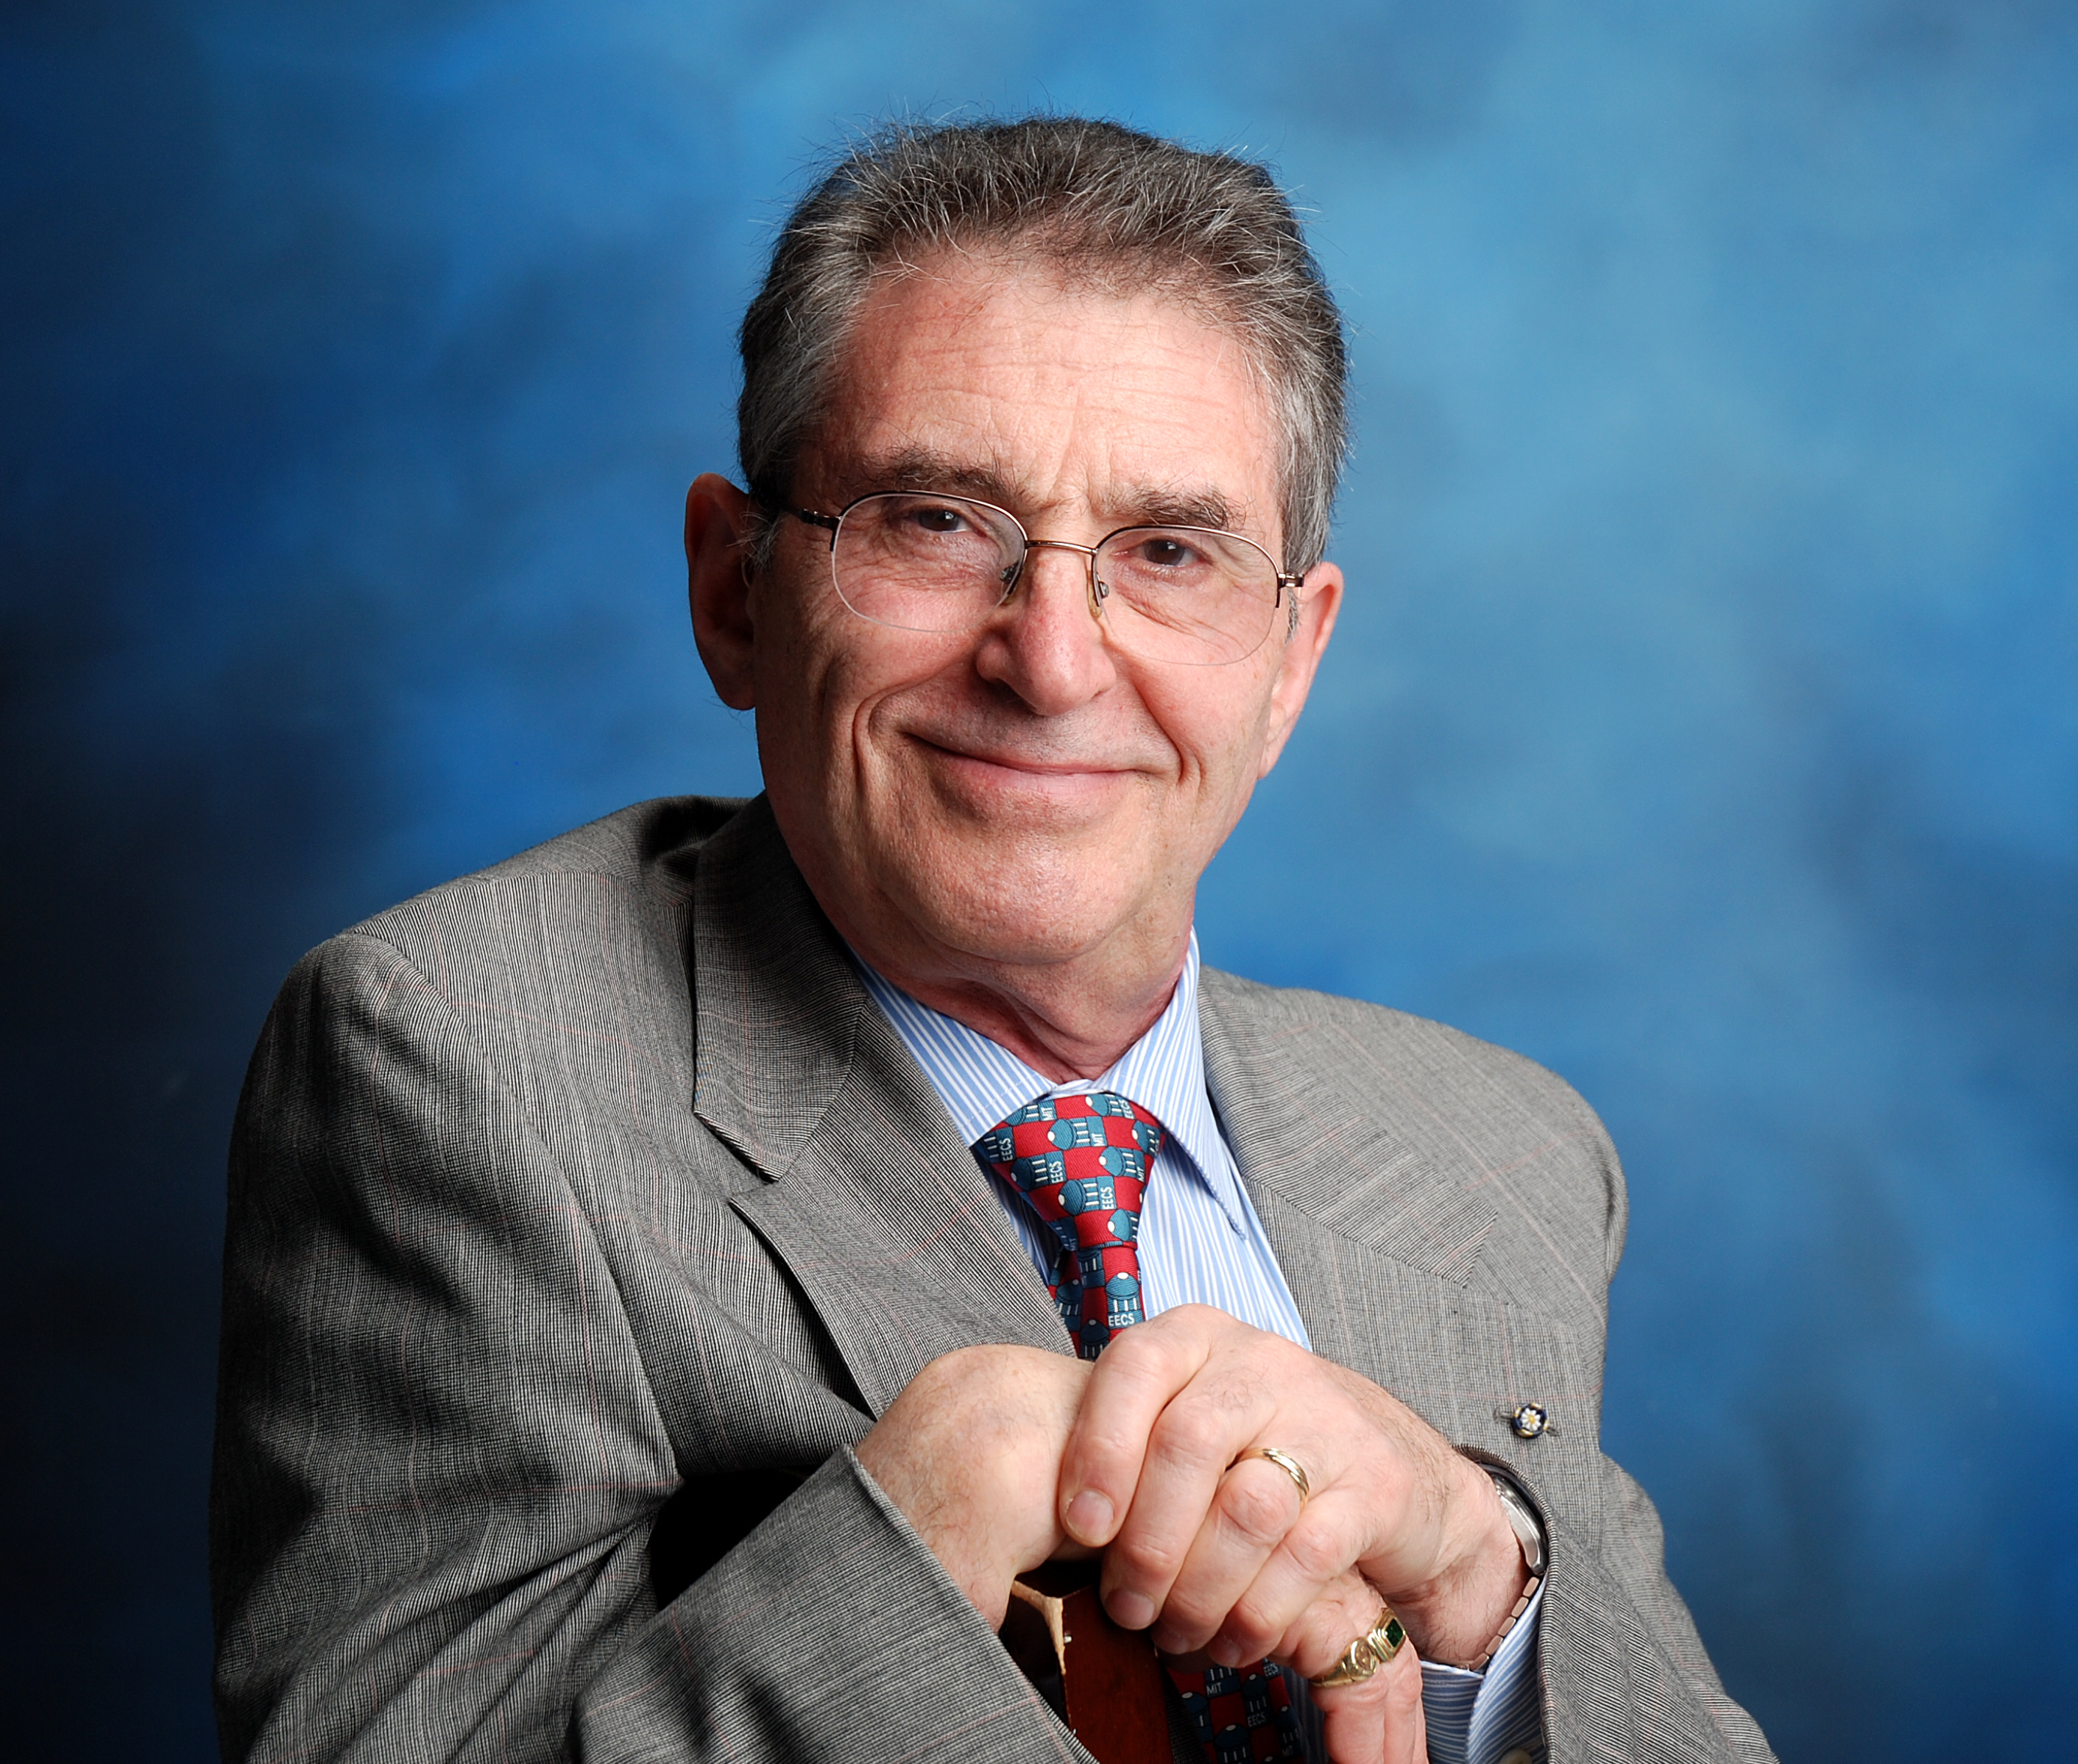
\includegraphics[height=2cm]{prologue/pix/MayerA_PortraitSimple152752.jpg}% 
  \quad %\vspace*{1ex}
  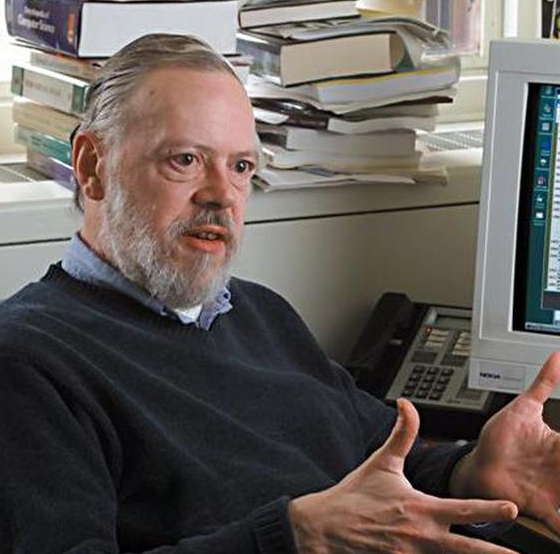
\includegraphics[height=2cm]{prologue/pix/ritchie.jpg}}% 
  \wrapcaption{\label{fig:mayer}\href{https://en.wikipedia.org/wiki/Albert_R._Meyer}{Albert Meyer b~1941} 与 \label{fig:ritchie}\href{https://en.wikipedia.org/wiki/Dennis_Ritchie}{Dennis Ritchie 1941--2011}}\index{Ritchie, D!picture}\index{Meyer, A!picture}
\end{wrapfigure}


%\margingraphic[l]{0.21\textwidth}{prologue/pix/ritchie.jpg}{\label{fig:ritchie}\href{https://en.wikipedia.org/wiki/Dennis_Ritchie}{Dennis Ritchie 1941--2011, inventor of C}}\index{Ritchie, D!picture}
Albert Meyer（阿尔伯特·迈耶）与 C 语言发明者 Dennis Ritchie（丹尼斯·里奇）研究了这一方向。我们将证明这个结论的一半：如果一个函数是原始递归的，那么我们可以只用有界循环来计算它。
具体做法是，在名为\citetext{\definend{LOOP 程序}}{%
  \protect\autocite{MeyerRitchie}}\index{LOOP program!language} 的语言中，为原始递归函数编写程序，
这种语言没有无界循环。
（其逆命题的证明超出了本书范围。）

% Picture from web page https://people.csail.mit.edu/meyer/; permission from A Meyer via email 2023-Feb-20 
%\margingraphic{0.21\textwidth}{prologue/pix/MayerA_PortraitSimple152752.jpg}{\label{fig:mayer}\href{https://en.wikipedia.org/wiki/Albert_R._Meyer}{Albert Meyer b~1941}}\index{Meyer, A!picture}
LOOP\index{LOOP program} 程序在一个带有寄存器的机器模型上执行，
寄存器 \codeinline{r0}、\codeinline{r1}、\ldots\ 可以存放自然数。
指令共有四种，我们使用 \codeinline{r0} 和 \codeinline{r1} 来描述它们：(i) \codeinline{r0 = 0}
将寄存器的内容设置为零，
(ii)~\codeinline{r0 = r0 + 1} 将寄存器的内容加一，
(iii)~\codeinline{r1 = r0} 将 \codeinline{r0} 的内容复制到 \codeinline{r1}，
而 \codeinline{r0} 保持不变，
以及 (iv)~\codeinline{loop r0 ... end}
重复执行一系列指令，
重复次数由该寄存器的值给定。
对于最后一种指令，`\codeinline{...}` 代表一个指令序列，它可以包含这四种语句中的任何一种，
包括嵌套的 \codeinline{loop}（该内层循环自身又可能包含嵌套的 \codeinline{loop}，依此类推）。

举个例子，下面的 LOOP 程序结束时，寄存器 \codeinline{r0} 中的值为 $4$，
而 \codeinline{r1} 中的值为~$2$（循环内的缩进只是为了视觉清晰）。
注意，除非在运行程序前预装载了机器，否则寄存器的初始值都是零。
\lstinputlisting{\prfiles machines/simple.loop}

非常重要的是：在循环内部改变循环寄存器的内容，
并不会改变机器执行该循环的次数。
因此，下面的代码并不是一个无限循环。
\begin{lstlisting}
loop r0 
  r0 = r0 + 1
  end  
\end{lstlisting}
相反，
当循环结束时，\codeinline{r0} 中的值将是循环开始时的两倍。

为了将 LOOP 程序解释为计算函数，我们需要对输入和输出作一些约定。
对于一个接收 $n$ 个输入的函数，我们会将这 $n$ 个输入预装载到机器的前 $n$ 个寄存器中。
类似地，对于一个有 $m$ 个输出的函数，我们取前 $m$ 个寄存器的最终值作为这 $m$ 个输出。

根据此约定，这个 LOOP 程序计算的是双输入、单输出的加法函数 $\plus(x,y)=x+y$。
\lstinputlisting{\prfiles machines/plus.loop}
本书的源代码包中附带一个 Racket 程序 \codeinline{loop.rkt}，它可以解释 LOOP 代码。
下面是运行该代码的一个调用示例。\footnote{%
  Racket 版本 8.2。}
\begin{lstlisting}
jim@millstone:src/scheme/prologue$ ./loop.rkt -f machines/plus.loop -p "3 2" -s
r0=3 r1=2
  --start loop of 2 repetitions--
  r0=4 r1=2
  r0=5 r1=2
  --end loop--
5
\end{lstlisting}  % $
程序的选项有：\codeinline{p} 将寄存器 \codeinline{r0} 和~\codeinline{r1} 预装载为 $3$ 和 $2$，
而 \codeinline{s} 则显示计算过程中每一步的寄存器状态。
默认情况下，模拟器返回第一个寄存器的值，此处为~$5$。

这个 LOOP 程序计算的是乘法函数 $\product(x,y)=x\cdot y$。
\lstinputlisting{\prfiles machines/product.loop}
它包含一个嵌套循环。
\begin{lstlisting}
jim@millstone:src/scheme/prologue$ ./loop.rkt -f machines/product.loop -p "3 2" -s
r0=3 r1=2
r0=3 r1=2 r2=2
r0=3 r1=3 r2=2
r0=0 r1=3 r2=2
  --start loop of 2 repetitions--
    --start loop of 3 repetitions--
    r0=1 r1=3 r2=2
    r0=2 r1=3 r2=2
    r0=3 r1=3 r2=2
    --end loop--
    --start loop of 3 repetitions--
    r0=4 r1=3 r2=2
    r0=5 r1=3 r2=2
    r0=6 r1=3 r2=2
    --end loop--
  --end loop--
6
\end{lstlisting}  % $

再看两个例子。
这个程序计算前驱函数 $\pred(x)$，
\lstinputlisting{\prfiles machines/pred.loop}
当 $x$ 不等于~$0$ 时，它等于 $x-1$；当 $x$ 等于~$0$ 时，它等于~$0$。
\begin{lstlisting}
jim@millstone:src/scheme/prologue$ ./loop.rkt -f machines/pred.loop -p "3" -s
r0=3
  --start loop of 3 repetitions--
  r0=3 r1=0 r2=0
  r0=3 r1=1 r2=0
  r0=3 r1=1 r2=1
  r0=3 r1=2 r2=1
  r0=3 r1=2 r2=2
  r0=3 r1=3 r2=2
  --end loop--
r0=2 r1=3 r2=2
2
\end{lstlisting}  % $
而这个程序利用前驱函数来计算截断减法 $x\dotminus y$，
\lstinputlisting{\prfiles machines/proper-sub.loop}
当 $y$ 不大于 $x$ 时，它等于 $x-y$；否则，结果为~$0$。
\begin{lstlisting}
jim@millstone:src/scheme/prologue$ ./loop.rkt -f machines/proper-sub.loop -p "3 2" -s
r0=3 r1=2
  --start loop of 2 repetitions--
  r0=3 r1=2 r3=0
    --start loop of 3 repetitions--
    r0=3 r1=2 r2=0 r3=0
    r0=3 r1=2 r2=0 r3=1
    r0=3 r1=2 r2=1 r3=1
    r0=3 r1=2 r2=1 r3=2
    r0=3 r1=2 r2=2 r3=2
    r0=3 r1=2 r2=2 r3=3
    --end loop--
  r0=2 r1=2 r2=2 r3=3
  r0=2 r1=2 r2=2 r3=0
    --start loop of 2 repetitions--
    r0=2 r1=2 r2=0 r3=0
    r0=2 r1=2 r2=0 r3=1
    r0=2 r1=2 r2=1 r3=1
    r0=2 r1=2 r2=1 r3=2
    --end loop--
  r0=1 r1=2 r2=1 r3=2
  --end loop--
1
\end{lstlisting}  % $

最后，这个例子展示了一个有多个输出的程序。
\lstinputlisting{\prfiles machines/rotate-shift-right.loop}
程序的 \codeinline{o} 选项让我们可以显示三个寄存器，而不是默认的一个，
\begin{lstlisting}
jim@millstone$ ./loop.rkt -f machines/rotate-shift-right.loop -p "1 2 3" -o 3
3 1 2
\end{lstlisting}  % $
（我们通过不使用 \codeinline{s} 选项避免了显示计算步骤）。

现在我们准备证明，对于每个原始递归函数，都存在一个计算它的 LOOP 程序。
策略是首先展示如何计算初始函数，然后展示如何实现函数复合与原始递归这两种组合运算。

零函数~$\zero(x)=0$ 可以用单行 LOOP 程序 \codeinline{r0 = 0} 来计算。
后继函数 $\successor(x)=x+1$ 可以用单行程序 \codeinline{r0 = r0 + 1} 来计算。
投影 $\projection_i(x_0,\ldots x_i,\ldots x_{n-1})=x_i$
可以用 \codeinline{r0 = r}$i$ 来计算。

两个函数的复合运算很容易。
设 $g(x_0,\ldots\, x_n)$ 和 $f(y_0,\ldots\, y_m)$
分别由 LOOP 程序 $P_g$ 和 $P_f$ 计算。
假设函数复合 $\composed{f}{g}$ 的参数对应是恰当的，即
$g$ 是一个 $m$ 输出函数，与 $f$ 的输入数量相匹配。
那么将这两个程序连接起来——也就是让 $P_g$ 的指令之后紧接着
$P_f$ 的指令——就得到了复合运算所需的 LOOP 程序，
因为它使用 $g$ 的输出作为输入来执行 $f$ 的计算。

一般化的复合运算从
\begin{equation*}
 f(x_0,\ldots\, x_n),
 \quad
 h_0(y_{0,0},\ldots\, y_{0,m_0}),
 \quad\ldots\quad
 h_n(y_{n,0},\ldots\, y_{n,m_n})
\end{equation*}
% $f(x_0,\ldots,x_n)$ 
% and $h_0(y_{0,0},\ldots,y_{0,m_0})$, \ldots  $h_n(y_{n,0},\ldots,y_{n,m_n})$
开始，并产生
$f(h_0(y_{0,0},\ldots y_{0,m_0}),\ldots h_n(y_{n,0},\ldots y_{n,m_n}))$。
这比两个函数的情况需要多一些思考。
问题在于，如果我们把输入 $y_{0,0}$, \ldots{} $y_{n,m_n}$ 装载到寄存器
\codeinline{r0}, \codeinline{r1}, \ldots{} 中，
然后立即开始计算 $h_0$，就会有覆盖后续函数（如 $h_1$）输入的危险。
例如，上面的 \codeinline{rotate-shift-right.loop} 就使用了一个额外的寄存器
\codeinline{r3}，它不在存储输入所用的寄存器之列。

因此我们必须把这些输入移开。
设 $P_f$, $P_{h_0}$, \ldots{} $P_{h_n}$
是计算这些函数的 LOOP 程序。
每个程序都使用有限数量的寄存器，
因此存在一个足够大的数~$j$，使得这些程序都不使用
寄存器~$j$。
根据定义，用来计算复合的程序~$P$
接收的输入序列从编号为~$0$ 的寄存器开始。
第一步是将这些输入复制到从寄存器~$j$ 开始的位置。
% (the final member will be copied to just before
% the register numbered $(m_0+1)+\cdots+(m_n+1)$).
接下来，将寄存器~$j$ 下方的寄存器清零，
将 $h_0$ 的参数向下复制到以 \codeinline{r0} 开头的位置，
然后运行程序 $P_{h_0}$。
当它执行完毕后，将其输出复制到编号为
$j+m_0+\cdots+ m_n+1$
的寄存器中。
对其他 $h_i$ 做类似处理。
最后，将这些输出向下复制到初始的寄存器，将剩余的寄存器清零，并运行 $P_f$。

另一个组合操作是原始递归。
\begin{equation*}
  f(x_0,\ldots\, x_{k-1},y)=
  \begin{cases}
    g(x_0,\ldots\, x_{k-1}) &\case{若 $y=0$}   \\
    h(f(x_0,\ldots\, x_{k-1},z),\,x_0,\ldots\, x_{k-1},\,z)
      &\case{若 $y=\successor(z)$}
  \end{cases}
\end{equation*}
假设我们有 LOOP 程序 $P_g$ 和~$P_h$。
所需的寄存器交换与复合运算的情况类似，所以我们就不再赘述了。
程序 $P_f$ 从运行 $P_g$ 开始。
然后它将一个新寄存器设为 $0$；称这个寄存器为~\codeinline{t}。
现在它进入一个基于寄存器~\codeinline{y} 的循环
（即，每次循环依次按 $y$, $y-1$ 等倒计数）。
循环体通过运行~$P_h$ 来计算
$f(x_0,\ldots\, x_{k-1},t+1)=h(f(x_0,\ldots x_{k-1},t),\,x_0,\ldots\, x_{k-1},t)$，
然后递增~\codeinline{t}。
至此论证完毕。

我们以关于 \codeinline{loop.rkt} 一个有趣方面的备注作为结尾，
\citetext{它是 LOOP 的解释器}{%
  改编自 \autocite{Schnieder}}。
它的工作原理是将上面使用的类 C 语法替换为类 LISP 的语法。
例如，解释器将左侧的字符串输入转换为右侧的字符串。


\begin{center}
  \begin{minipage}[t]{0.45\linewidth}
\begin{lstlisting}
r1 = r1 + 1
loop r1
  r0 = r0 + 1
  end
\end{lstlisting}
  \end{minipage}
  \qquad
  \begin{minipage}[t]{0.45\linewidth}
\begin{lstlisting}
((incr r1) (loop r1 (incr r0)))      
\end{lstlisting}
  \end{minipage}
\end{center}


这种转换的好处是括号能自动将每个 \codeinline{loop} 的开头与其
\codeinline{end} 匹配，
这样我们就不必在解释器中编写包含栈的代码来跟踪循环嵌套。
对于右侧的字符串，\codeinline{loop.rkt} 通过将其传入 \codeinline{eval} 命令来运行并计算出结果。

% ......................................
\begin{exercises}


\begin{exercise}
编写一个 LOOP 程序，输入两个数并交换它们，
使得 $x,y$ 变为 $y,x$。   
\begin{answer}\verified
代码如下。
\lstinputlisting{scheme/prologue/machines/swap-two.loop} 
这是一个示例调用。
\begin{lstlisting}
jim@millstone:src/scheme/prologue$ ./loop.rkt -f machines/swap-two.loop -p "1 2 3" -o 2
2 1
\end{lstlisting}
\end{answer} % $
\end{exercise}

\begin{exercise}
论证如果允许像 \codeinline{r0 = r0 + 2} 这样的语句，
或者像 \codeinline{r0 = 1} 这样的语句，LOOP 语言并不会变得更强大。    
\begin{answer}\verified
我们可以用连续两次递增来实现第一种的效果，
而第二种的效果可以通过先清零再递增来实现。  
\end{answer}
\end{exercise}

\begin{exercise}
程序 \codeinline{rotate-shift-right.loop} 输入 
三个数，输出三个数，
并将输入右移（第三个数最终进入第一个寄存器）。
编写一个三输入/三输出的程序，实现左循环移位。
同时编写复合这两个程序的程序。
它计算什么？
\begin{answer}\verified
左旋转代码是对右旋转代码的改编。
\lstinputlisting{scheme/prologue/machines/rotate-shift-left.loop} 
这是一个示例调用。
\begin{lstlisting}
jim@millstone:src/scheme/prologue$ ./loop.rkt -f machines/rotate-shift-left.loop -p "1 2 3" -o 3
2 3 1
\end{lstlisting}  % $
将两者组合起来得到如下程序。
\lstinputlisting{scheme/prologue/machines/concatenate-rotations.loop} 
这是一个示例调用。
\begin{lstlisting}
jim@millstone:src/scheme/prologue$ ./loop.rkt -f machines/concatenate-rotations.loop -p "1 2 3" -o 3
1 2 3
\end{lstlisting}  % $
\end{answer} 
\end{exercise}

\begin{exercise}
在 Ackermann 函数中，
在运算 $\plus(x,y)$ 和 $\product(x,y)$ 之后是 $\power(x,y)$。
为它写一个 LOOP 程序。
\begin{answer}\verified
下面是一个程序。
\lstinputlisting{scheme/prologue/machines/power.loop} 
这里是两个示例调用。
\begin{lstlisting}
jim@millstone:src/scheme/prologue$ ./loop.rkt -f machines/power.loop -p "3 2"
9
jim@millstone:src/scheme/prologue$ ./loop.rkt -f machines/power.loop -p "3 0"
1
\end{lstlisting}
\end{answer} % $
\end{exercise}

\begin{exercise}
如果你试图在 Racket 的循环内部修改循环变量，会发生什么？
例如，下面这两个程序的行为分别是什么？
\begin{center}
  \begin{minipage}{0.4\linewidth}
    \begin{lstlisting}
(for ([i (in-range 5)])
  (set! i 1)
  (displayln (~a "i=" i)))
\end{lstlisting}
  \end{minipage}
  \qquad
  \begin{minipage}{0.4\linewidth}
    \begin{lstlisting}
(for ([i (in-range 5)])
  (displayln (~a "i=" i))
  (set! i 1))
\end{lstlisting}
  \end{minipage}
\end{center}
\begin{answer}
第一个程序是这样的；请注意它运行了五次。
\begin{lstlisting}
 > (for ([i (in-range 5)])
    (set! i 1)
    (displayln (~a "i=" i)))
i=1
i=1
i=1
i=1
i=1    
\end{lstlisting}
第二个程序是这样的。
\begin{lstlisting}
> (for ([i (in-range 5)])
    (displayln (~a "i=" i))
    (set! i 1))
i=0
i=1
i=2
i=3
i=4     
\end{lstlisting}
\end{answer}
\end{exercise}

\end{exercises}
\index{LOOP program|)}
